\documentclass{beamer}
\usepackage{amsmath}

\definecolor{uwpurple}{RGB}{51,0,111}
\definecolor{uwgold}{RGB}{232,211,162}
\definecolor{uwmetallicgold}{RGB}{145,123,76}
\definecolor{cffffff}{RGB}{255,255,255}

\usetheme{Frankfurt}
\setbeamertemplate{navigation symbols}{}
\setbeamercolor{section in head/foot}{bg=uwpurple}
\setbeamercolor{structure}{fg=uwmetallicgold}
\setbeamercolor{block title}{bg=uwpurple}
\addtobeamertemplate{block begin}{
  \setbeamercolor{itemize item}{fg=uwpurple}
  \setbeamercolor{itemize subitem}{fg=uwpurple}
  \setbeamercolor{enumerate item}{fg=uwpurple}
  \setbeamercolor{enumerate subitem}{fg=uwpurple}
}{}
\setbeamertemplate{itemize items}[default]
\setbeamertemplate{enumerate items}[default]

\usepackage{tikz}

\title{Parallel Markov Chain Monte Carlo for Nonparametric Mixture Models}
\author{Arman Bilge \\ \small\href{mailto:abilge@uw.edu}{\texttt{abilge@uw.edu}}}
\institute{Statistics Department, University of Washington \\ Computational Biology Program, Fred Hutchinson Cancer Research Center}
\date{April 6, 2017}

\frenchspacing
\begin{document}

  \frame{\titlepage}

  \section{Motivation}

  \stepcounter{subsection}
  \begin{frame}{Dirichlet Process}

    \begin{itemize}
      \item Model data that may repeat previous values
      \item \emph{Rich get richer}
      \item Parameters: base distribution $H$ and concentration $\alpha > 0$
    \end{itemize}

    \begin{block}{Simulation}
      \begin{enumerate}
        \item Sample $X_1 \sim H$
        \item For $n > 1$ let
        \begin{equation*}
          \begin{cases}
            X_n \sim H & \text{ with probability } \frac{\alpha}{\alpha + n - 1} \\
            X_n = x & \text{ with probability } \frac{n_x}{\alpha + n - 1}
          \end{cases}
        \end{equation*}
        where $n_x$ is number of previous occurrences of $x$
      \end{enumerate}
    \end{block}

  \end{frame}

  \stepcounter{subsection}
  \begin{frame}{Dirichlet Process}
    \centering
    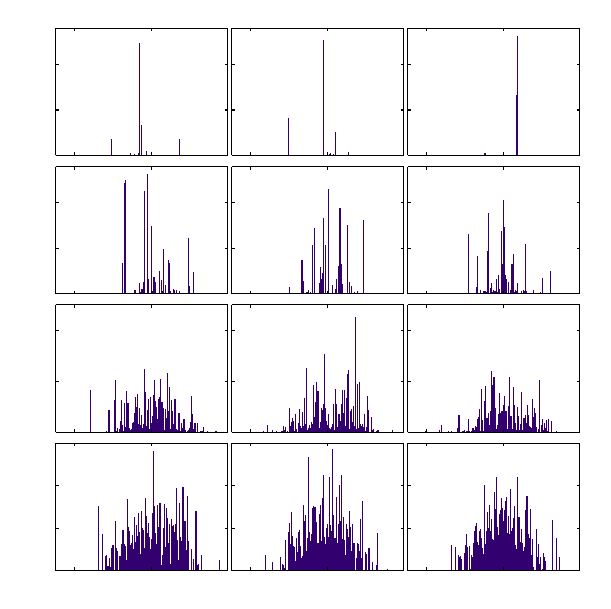
\begin{tikzpicture}[y=0.80pt, x=0.80pt, yscale=-1.000000, xscale=1.000000, inner sep=0pt, outer sep=0pt, scale=0.35]
          % \path[fill=cffffff] (0.0000,720.0000) -- (720.0000,720.0000) --
    %   (720.0000,0.0000) -- (0.0000,0.0000) -- cycle;
    %   \path[fill=cffffff] (38.6781,165.9500) -- (260.8210,165.9500) --
    %     (260.8210,1.8000) -- (38.6781,1.8000) -- cycle;
      \path[draw=uwpurple,line cap=rect] (202.1840,165.9500) -- (202.1840,165.8610);
      \path[draw=uwpurple,line cap=rect] (146.9910,165.9500) -- (146.9910,22.0686);
      \path[draw=uwpurple,line cap=rect] (149.0540,165.9500) -- (149.0540,127.5580);
      \path[draw=uwpurple,line cap=rect] (135.6070,165.9500) -- (135.6070,163.9040);
      \path[draw=uwpurple,line cap=rect] (198.1800,165.9500) -- (198.1800,145.1750);
      \path[draw=uwpurple,line cap=rect] (111.2410,165.9500) -- (111.2410,145.8600);
      \path[draw=uwpurple,line cap=rect] (157.8350,165.9500) -- (157.8350,165.7300);
      \path[draw=uwpurple,line cap=rect] (140.4230,165.9500) -- (140.4230,164.2630);
      \path[draw=uwpurple,line cap=rect] (155.4790,165.9500) -- (155.4790,160.9080);
      \path[draw=uwpurple,line cap=rect] (175.1820,165.9500) -- (175.1820,165.8870);
      \path[draw=uwpurple,line cap=rect] (145.1300,165.9500) -- (145.1300,163.9520);
      \path[draw=uwpurple,line cap=rect] (141.2290,165.9500) -- (141.2290,165.7770);
      \path[draw=uwpurple,line cap=rect] (203.0590,165.9500) -- (203.0590,165.9410);
      \path[draw=uwpurple,line cap=rect] (180.4070,165.9500) -- (180.4070,165.9470);
      \path[draw=uwpurple,line cap=rect] (166.8030,165.9500) -- (166.8030,165.9450);
      \path[draw=uwpurple,line cap=rect] (213.9310,165.9500) -- (213.9310,165.9300);
      \path[draw=uwmetallicgold,line cap=rect] (111.2410,165.9500) -- (213.9310,165.9500);
            \begin{scope}[shift={(63.36071,165.95)},draw=black,line width=0.400pt]
              \path[draw=black,line width=0.400pt] (0.0000,0.0000) -- (0.0000,-4.0000);
            \end{scope}
            \begin{scope}[shift={(63.36071,1.8)},draw=black,line width=0.400pt]
              \path[draw=black,line width=0.400pt] (0.0000,0.0000) -- (0.0000,4.0000);
            \end{scope}
            \begin{scope}[shift={(162.09103,165.95)},draw=black,line width=0.400pt]
              \path[draw=black,line width=0.400pt] (0.0000,0.0000) -- (0.0000,-4.0000);
            \end{scope}
            \begin{scope}[shift={(162.09103,1.8)},draw=black,line width=0.400pt]
              \path[draw=black,line width=0.400pt] (0.0000,0.0000) -- (0.0000,4.0000);
            \end{scope}
            \begin{scope}[shift={(260.82135,165.95)},draw=black,line width=0.400pt]
              \path[draw=black,line width=0.400pt] (0.0000,0.0000) -- (0.0000,-4.0000);
            \end{scope}
            \begin{scope}[shift={(260.82135,1.8)},draw=black,line width=0.400pt]
              \path[draw=black,line width=0.400pt] (0.0000,0.0000) -- (0.0000,4.0000);
            \end{scope}
            \begin{scope}[shift={(38.67813,165.95)},draw=black,line width=0.400pt]
              \path[draw=black,line width=0.400pt] (0.0000,0.0000) -- (4.0000,0.0000);
            \end{scope}
            \begin{scope}[shift={(260.82135,165.95)},draw=black,line width=0.400pt]
              \path[draw=black,line width=0.400pt] (0.0000,0.0000) -- (-4.0000,0.0000);
            \end{scope}
          \begin{scope}[shift={(9.5475,169.26125)},xscale=0.120,yscale=-0.120]
              \path (31.7812,66.4062) .. controls (26.7083,66.4062) and (22.8906,63.9062) ..
                (20.3281,58.9062) .. controls (17.7760,53.9167) and (16.5000,46.4063) ..
                (16.5000,36.3750) .. controls (16.5000,26.3854) and (17.7760,18.8906) ..
                (20.3281,13.8906) .. controls (22.8906,8.8906) and (26.7083,6.3906) ..
                (31.7812,6.3906) .. controls (36.8958,6.3906) and (40.7291,8.8906) ..
                (43.2812,13.8906) .. controls (45.8437,18.8906) and (47.1250,26.3854) ..
                (47.1250,36.3750) .. controls (47.1250,46.4063) and (45.8437,53.9167) ..
                (43.2812,58.9062) .. controls (40.7291,63.9062) and (36.8958,66.4062) ..
                (31.7812,66.4062)(31.7812,74.2188) .. controls (39.9583,74.2188) and
                (46.2031,70.9844) .. (50.5156,64.5156) .. controls (54.8281,58.0573) and
                (56.9844,48.6771) .. (56.9844,36.3750) .. controls (56.9844,24.1042) and
                (54.8281,14.7344) .. (50.5156,8.2656) .. controls (46.2031,1.8073) and
                (39.9583,-1.4219) .. (31.7812,-1.4219) .. controls (23.6145,-1.4219) and
                (17.3750,1.8073) .. (13.0625,8.2656) .. controls (8.7500,14.7344) and
                (6.5938,24.1042) .. (6.5938,36.3750) .. controls (6.5938,48.6771) and
                (8.7500,58.0573) .. (13.0625,64.5156) .. controls (17.3750,70.9844) and
                (23.6145,74.2188) .. (31.7812,74.2188);
            \begin{scope}[shift={(63.62305,0)}]
              \path (10.6875,12.4062) -- (21.0000,12.4062) -- (21.0000,0.0000) --
                (10.6875,0.0000) -- cycle;
            \end{scope}
            \begin{scope}[shift={(95.41016,0)}]
              \path (31.7812,66.4062) .. controls (26.7083,66.4062) and (22.8906,63.9062) ..
                (20.3281,58.9062) .. controls (17.7760,53.9167) and (16.5000,46.4063) ..
                (16.5000,36.3750) .. controls (16.5000,26.3854) and (17.7760,18.8906) ..
                (20.3281,13.8906) .. controls (22.8906,8.8906) and (26.7083,6.3906) ..
                (31.7812,6.3906) .. controls (36.8958,6.3906) and (40.7291,8.8906) ..
                (43.2812,13.8906) .. controls (45.8437,18.8906) and (47.1250,26.3854) ..
                (47.1250,36.3750) .. controls (47.1250,46.4063) and (45.8437,53.9167) ..
                (43.2812,58.9062) .. controls (40.7291,63.9062) and (36.8958,66.4062) ..
                (31.7812,66.4062)(31.7812,74.2188) .. controls (39.9583,74.2188) and
                (46.2031,70.9844) .. (50.5156,64.5156) .. controls (54.8281,58.0573) and
                (56.9844,48.6771) .. (56.9844,36.3750) .. controls (56.9844,24.1042) and
                (54.8281,14.7344) .. (50.5156,8.2656) .. controls (46.2031,1.8073) and
                (39.9583,-1.4219) .. (31.7812,-1.4219) .. controls (23.6145,-1.4219) and
                (17.3750,1.8073) .. (13.0625,8.2656) .. controls (8.7500,14.7344) and
                (6.5938,24.1042) .. (6.5938,36.3750) .. controls (6.5938,48.6771) and
                (8.7500,58.0573) .. (13.0625,64.5156) .. controls (17.3750,70.9844) and
                (23.6145,74.2188) .. (31.7812,74.2188);
            \end{scope}
            \begin{scope}[shift={(159.0332,0)}]
              \path (31.7812,66.4062) .. controls (26.7083,66.4062) and (22.8906,63.9062) ..
                (20.3281,58.9062) .. controls (17.7760,53.9167) and (16.5000,46.4063) ..
                (16.5000,36.3750) .. controls (16.5000,26.3854) and (17.7760,18.8906) ..
                (20.3281,13.8906) .. controls (22.8906,8.8906) and (26.7083,6.3906) ..
                (31.7812,6.3906) .. controls (36.8958,6.3906) and (40.7291,8.8906) ..
                (43.2812,13.8906) .. controls (45.8437,18.8906) and (47.1250,26.3854) ..
                (47.1250,36.3750) .. controls (47.1250,46.4063) and (45.8437,53.9167) ..
                (43.2812,58.9062) .. controls (40.7291,63.9062) and (36.8958,66.4062) ..
                (31.7812,66.4062)(31.7812,74.2188) .. controls (39.9583,74.2188) and
                (46.2031,70.9844) .. (50.5156,64.5156) .. controls (54.8281,58.0573) and
                (56.9844,48.6771) .. (56.9844,36.3750) .. controls (56.9844,24.1042) and
                (54.8281,14.7344) .. (50.5156,8.2656) .. controls (46.2031,1.8073) and
                (39.9583,-1.4219) .. (31.7812,-1.4219) .. controls (23.6145,-1.4219) and
                (17.3750,1.8073) .. (13.0625,8.2656) .. controls (8.7500,14.7344) and
                (6.5938,24.1042) .. (6.5938,36.3750) .. controls (6.5938,48.6771) and
                (8.7500,58.0573) .. (13.0625,64.5156) .. controls (17.3750,70.9844) and
                (23.6145,74.2188) .. (31.7812,74.2188);
            \end{scope}
          \end{scope}
            \begin{scope}[shift={(38.67813,107.325)},draw=black,line width=0.400pt]
              \path[draw=black,line width=0.400pt] (0.0000,0.0000) -- (4.0000,0.0000);
            \end{scope}
            \begin{scope}[shift={(260.82135,107.325)},draw=black,line width=0.400pt]
              \path[draw=black,line width=0.400pt] (0.0000,0.0000) -- (-4.0000,0.0000);
            \end{scope}
          \begin{scope}[shift={(9.79875,110.63625)},xscale=0.120,yscale=-0.120]
              \path (31.7812,66.4062) .. controls (26.7083,66.4062) and (22.8906,63.9062) ..
                (20.3281,58.9062) .. controls (17.7760,53.9167) and (16.5000,46.4063) ..
                (16.5000,36.3750) .. controls (16.5000,26.3854) and (17.7760,18.8906) ..
                (20.3281,13.8906) .. controls (22.8906,8.8906) and (26.7083,6.3906) ..
                (31.7812,6.3906) .. controls (36.8958,6.3906) and (40.7291,8.8906) ..
                (43.2812,13.8906) .. controls (45.8437,18.8906) and (47.1250,26.3854) ..
                (47.1250,36.3750) .. controls (47.1250,46.4063) and (45.8437,53.9167) ..
                (43.2812,58.9062) .. controls (40.7291,63.9062) and (36.8958,66.4062) ..
                (31.7812,66.4062)(31.7812,74.2188) .. controls (39.9583,74.2188) and
                (46.2031,70.9844) .. (50.5156,64.5156) .. controls (54.8281,58.0573) and
                (56.9844,48.6771) .. (56.9844,36.3750) .. controls (56.9844,24.1042) and
                (54.8281,14.7344) .. (50.5156,8.2656) .. controls (46.2031,1.8073) and
                (39.9583,-1.4219) .. (31.7812,-1.4219) .. controls (23.6145,-1.4219) and
                (17.3750,1.8073) .. (13.0625,8.2656) .. controls (8.7500,14.7344) and
                (6.5938,24.1042) .. (6.5938,36.3750) .. controls (6.5938,48.6771) and
                (8.7500,58.0573) .. (13.0625,64.5156) .. controls (17.3750,70.9844) and
                (23.6145,74.2188) .. (31.7812,74.2188);
            \begin{scope}[shift={(63.62305,0)}]
              \path (10.6875,12.4062) -- (21.0000,12.4062) -- (21.0000,0.0000) --
                (10.6875,0.0000) -- cycle;
            \end{scope}
            \begin{scope}[shift={(95.41016,0)}]
              \path (19.1875,8.2969) -- (53.6094,8.2969) -- (53.6094,0.0000) --
                (7.3281,0.0000) -- (7.3281,8.2969) .. controls (11.0677,12.1719) and
                (16.1667,17.3698) .. (22.6250,23.8906) .. controls (29.0937,30.4219) and
                (33.1562,34.6354) .. (34.8125,36.5312) .. controls (37.9688,40.0729) and
                (40.1719,43.0729) .. (41.4219,45.5312) .. controls (42.6823,47.9896) and
                (43.3125,50.4063) .. (43.3125,52.7812) .. controls (43.3125,56.6563) and
                (41.9531,59.8125) .. (39.2344,62.2500) .. controls (36.5156,64.6979) and
                (32.9739,65.9219) .. (28.6094,65.9219) .. controls (25.5157,65.9219) and
                (22.2500,65.3854) .. (18.8125,64.3125) .. controls (15.3854,63.2396) and
                (11.7188,61.6094) .. (7.8125,59.4219) -- (7.8125,69.3906) .. controls
                (11.7812,70.9843) and (15.4896,72.1875) .. (18.9375,73.0000) .. controls
                (22.3958,73.8125) and (25.5573,74.2188) .. (28.4219,74.2188) .. controls
                (35.9740,74.2188) and (41.9948,72.3282) .. (46.4844,68.5469) .. controls
                (50.9740,64.7760) and (53.2188,59.7344) .. (53.2188,53.4219) .. controls
                (53.2188,50.4219) and (52.6563,47.5781) .. (51.5312,44.8906) .. controls
                (50.4167,42.2135) and (48.3750,39.0521) .. (45.4062,35.4062) .. controls
                (44.5937,34.4583) and (42.0052,31.7292) .. (37.6406,27.2188) .. controls
                (33.2865,22.7083) and (27.1354,16.4010) .. (19.1875,8.2969);
            \end{scope}
            \begin{scope}[shift={(159.0332,0)}]
              \path (10.7969,72.9062) -- (49.5156,72.9062) -- (49.5156,64.5938) --
                (19.8281,64.5938) -- (19.8281,46.7344) .. controls (21.2552,47.2240) and
                (22.6823,47.5886) .. (24.1094,47.8281) .. controls (25.5469,48.0677) and
                (26.9844,48.1875) .. (28.4219,48.1875) .. controls (36.5573,48.1875) and
                (43.0000,45.9583) .. (47.7500,41.5000) .. controls (52.5104,37.0417) and
                (54.8906,31.0052) .. (54.8906,23.3906) .. controls (54.8906,15.5469) and
                (52.4479,9.4479) .. (47.5625,5.0938) .. controls (42.6771,0.7500) and
                (35.7917,-1.4219) .. (26.9062,-1.4219) .. controls (23.8437,-1.4219) and
                (20.7240,-1.1615) .. (17.5469,-0.6406) .. controls (14.3802,-0.1198) and
                (11.1042,0.6615) .. (7.7188,1.7031) -- (7.7188,11.6250) .. controls
                (10.6458,10.0313) and (13.6719,8.8438) .. (16.7969,8.0625) .. controls
                (19.9219,7.2812) and (23.2240,6.8906) .. (26.7031,6.8906) .. controls
                (32.3385,6.8906) and (36.7968,8.3698) .. (40.0781,11.3281) .. controls
                (43.3698,14.2864) and (45.0156,18.3073) .. (45.0156,23.3906) .. controls
                (45.0156,28.4635) and (43.3698,32.4792) .. (40.0781,35.4375) .. controls
                (36.7968,38.4062) and (32.3385,39.8906) .. (26.7031,39.8906) .. controls
                (24.0677,39.8906) and (21.4375,39.5989) .. (18.8125,39.0156) .. controls
                (16.1979,38.4323) and (13.5260,37.5208) .. (10.7969,36.2812) -- cycle;
            \end{scope}
          \end{scope}
            \begin{scope}[shift={(38.67813,48.7)},draw=black,line width=0.400pt]
              \path[draw=black,line width=0.400pt] (0.0000,0.0000) -- (4.0000,0.0000);
            \end{scope}
            \begin{scope}[shift={(260.82135,48.7)},draw=black,line width=0.400pt]
              \path[draw=black,line width=0.400pt] (0.0000,0.0000) -- (-4.0000,0.0000);
            \end{scope}
          \begin{scope}[shift={(9.5475,52.01125)},xscale=0.120,yscale=-0.120]
              \path (31.7812,66.4062) .. controls (26.7083,66.4062) and (22.8906,63.9062) ..
                (20.3281,58.9062) .. controls (17.7760,53.9167) and (16.5000,46.4063) ..
                (16.5000,36.3750) .. controls (16.5000,26.3854) and (17.7760,18.8906) ..
                (20.3281,13.8906) .. controls (22.8906,8.8906) and (26.7083,6.3906) ..
                (31.7812,6.3906) .. controls (36.8958,6.3906) and (40.7291,8.8906) ..
                (43.2812,13.8906) .. controls (45.8437,18.8906) and (47.1250,26.3854) ..
                (47.1250,36.3750) .. controls (47.1250,46.4063) and (45.8437,53.9167) ..
                (43.2812,58.9062) .. controls (40.7291,63.9062) and (36.8958,66.4062) ..
                (31.7812,66.4062)(31.7812,74.2188) .. controls (39.9583,74.2188) and
                (46.2031,70.9844) .. (50.5156,64.5156) .. controls (54.8281,58.0573) and
                (56.9844,48.6771) .. (56.9844,36.3750) .. controls (56.9844,24.1042) and
                (54.8281,14.7344) .. (50.5156,8.2656) .. controls (46.2031,1.8073) and
                (39.9583,-1.4219) .. (31.7812,-1.4219) .. controls (23.6145,-1.4219) and
                (17.3750,1.8073) .. (13.0625,8.2656) .. controls (8.7500,14.7344) and
                (6.5938,24.1042) .. (6.5938,36.3750) .. controls (6.5938,48.6771) and
                (8.7500,58.0573) .. (13.0625,64.5156) .. controls (17.3750,70.9844) and
                (23.6145,74.2188) .. (31.7812,74.2188);
            \begin{scope}[shift={(63.62305,0)}]
              \path (10.6875,12.4062) -- (21.0000,12.4062) -- (21.0000,0.0000) --
                (10.6875,0.0000) -- cycle;
            \end{scope}
            \begin{scope}[shift={(95.41016,0)}]
              \path (10.7969,72.9062) -- (49.5156,72.9062) -- (49.5156,64.5938) --
                (19.8281,64.5938) -- (19.8281,46.7344) .. controls (21.2552,47.2240) and
                (22.6823,47.5886) .. (24.1094,47.8281) .. controls (25.5469,48.0677) and
                (26.9844,48.1875) .. (28.4219,48.1875) .. controls (36.5573,48.1875) and
                (43.0000,45.9583) .. (47.7500,41.5000) .. controls (52.5104,37.0417) and
                (54.8906,31.0052) .. (54.8906,23.3906) .. controls (54.8906,15.5469) and
                (52.4479,9.4479) .. (47.5625,5.0938) .. controls (42.6771,0.7500) and
                (35.7917,-1.4219) .. (26.9062,-1.4219) .. controls (23.8437,-1.4219) and
                (20.7240,-1.1615) .. (17.5469,-0.6406) .. controls (14.3802,-0.1198) and
                (11.1042,0.6615) .. (7.7188,1.7031) -- (7.7188,11.6250) .. controls
                (10.6458,10.0313) and (13.6719,8.8438) .. (16.7969,8.0625) .. controls
                (19.9219,7.2812) and (23.2240,6.8906) .. (26.7031,6.8906) .. controls
                (32.3385,6.8906) and (36.7968,8.3698) .. (40.0781,11.3281) .. controls
                (43.3698,14.2864) and (45.0156,18.3073) .. (45.0156,23.3906) .. controls
                (45.0156,28.4635) and (43.3698,32.4792) .. (40.0781,35.4375) .. controls
                (36.7968,38.4062) and (32.3385,39.8906) .. (26.7031,39.8906) .. controls
                (24.0677,39.8906) and (21.4375,39.5989) .. (18.8125,39.0156) .. controls
                (16.1979,38.4323) and (13.5260,37.5208) .. (10.7969,36.2812) -- cycle;
            \end{scope}
            \begin{scope}[shift={(159.0332,0)}]
              \path (31.7812,66.4062) .. controls (26.7083,66.4062) and (22.8906,63.9062) ..
                (20.3281,58.9062) .. controls (17.7760,53.9167) and (16.5000,46.4063) ..
                (16.5000,36.3750) .. controls (16.5000,26.3854) and (17.7760,18.8906) ..
                (20.3281,13.8906) .. controls (22.8906,8.8906) and (26.7083,6.3906) ..
                (31.7812,6.3906) .. controls (36.8958,6.3906) and (40.7291,8.8906) ..
                (43.2812,13.8906) .. controls (45.8437,18.8906) and (47.1250,26.3854) ..
                (47.1250,36.3750) .. controls (47.1250,46.4063) and (45.8437,53.9167) ..
                (43.2812,58.9062) .. controls (40.7291,63.9062) and (36.8958,66.4062) ..
                (31.7812,66.4062)(31.7812,74.2188) .. controls (39.9583,74.2188) and
                (46.2031,70.9844) .. (50.5156,64.5156) .. controls (54.8281,58.0573) and
                (56.9844,48.6771) .. (56.9844,36.3750) .. controls (56.9844,24.1042) and
                (54.8281,14.7344) .. (50.5156,8.2656) .. controls (46.2031,1.8073) and
                (39.9583,-1.4219) .. (31.7812,-1.4219) .. controls (23.6145,-1.4219) and
                (17.3750,1.8073) .. (13.0625,8.2656) .. controls (8.7500,14.7344) and
                (6.5938,24.1042) .. (6.5938,36.3750) .. controls (6.5938,48.6771) and
                (8.7500,58.0573) .. (13.0625,64.5156) .. controls (17.3750,70.9844) and
                (23.6145,74.2188) .. (31.7812,74.2188);
            \end{scope}
          \end{scope}
      \path[draw=black] (38.6781,1.8000) -- (260.8210,1.8000);
      \path[draw=black] (260.8210,165.9500) -- (260.8210,1.8000);
      \path[draw=black] (38.6781,165.9500) -- (260.8210,165.9500);
      \path[draw=black] (38.6781,165.9500) -- (38.6781,1.8000);
      % \path[fill=cffffff] (265.7850,165.9500) -- (487.9290,165.9500) --
      %   (487.9290,1.8000) -- (265.7850,1.8000) -- cycle;
      \path[draw=uwpurple,line cap=rect] (384.0420,165.9500) -- (384.0420,17.6030);
      \path[draw=uwpurple,line cap=rect] (403.6780,165.9500) -- (403.6780,165.5510);
      \path[draw=uwpurple,line cap=rect] (396.9890,165.9500) -- (396.9890,164.5150);
      \path[draw=uwpurple,line cap=rect] (339.2850,165.9500) -- (339.2850,118.9950);
      \path[draw=uwpurple,line cap=rect] (393.8030,165.9500) -- (393.8030,162.9480);
      \path[draw=uwpurple,line cap=rect] (399.3190,165.9500) -- (399.3190,136.6970);
      \path[draw=uwpurple,line cap=rect] (392.2050,165.9500) -- (392.2050,164.3770);
      \path[draw=uwpurple,line cap=rect] (417.0770,165.9500) -- (417.0770,162.5280);
      \path[draw=uwpurple,line cap=rect] (373.8950,165.9500) -- (373.8950,165.8590);
      \path[draw=uwmetallicgold,line cap=rect] (339.2850,165.9500) -- (417.0770,165.9500);
            \begin{scope}[shift={(290.468,165.95)},draw=black,line width=0.400pt]
              \path[draw=black,line width=0.400pt] (0.0000,0.0000) -- (0.0000,-4.0000);
            \end{scope}
            \begin{scope}[shift={(290.468,1.8)},draw=black,line width=0.400pt]
              \path[draw=black,line width=0.400pt] (0.0000,0.0000) -- (0.0000,4.0000);
            \end{scope}
            \begin{scope}[shift={(389.19832,165.95)},draw=black,line width=0.400pt]
              \path[draw=black,line width=0.400pt] (0.0000,0.0000) -- (0.0000,-4.0000);
            \end{scope}
            \begin{scope}[shift={(389.19832,1.8)},draw=black,line width=0.400pt]
              \path[draw=black,line width=0.400pt] (0.0000,0.0000) -- (0.0000,4.0000);
            \end{scope}
            \begin{scope}[shift={(487.92865,165.95)},draw=black,line width=0.400pt]
              \path[draw=black,line width=0.400pt] (0.0000,0.0000) -- (0.0000,-4.0000);
            \end{scope}
            \begin{scope}[shift={(487.92865,1.8)},draw=black,line width=0.400pt]
              \path[draw=black,line width=0.400pt] (0.0000,0.0000) -- (0.0000,4.0000);
            \end{scope}
            \begin{scope}[shift={(265.78542,165.95)},draw=black,line width=0.400pt]
              \path[draw=black,line width=0.400pt] (0.0000,0.0000) -- (4.0000,0.0000);
            \end{scope}
            \begin{scope}[shift={(487.92865,165.95)},draw=black,line width=0.400pt]
              \path[draw=black,line width=0.400pt] (0.0000,0.0000) -- (-4.0000,0.0000);
            \end{scope}
            \begin{scope}[shift={(265.78542,107.325)},draw=black,line width=0.400pt]
              \path[draw=black,line width=0.400pt] (0.0000,0.0000) -- (4.0000,0.0000);
            \end{scope}
            \begin{scope}[shift={(487.92865,107.325)},draw=black,line width=0.400pt]
              \path[draw=black,line width=0.400pt] (0.0000,0.0000) -- (-4.0000,0.0000);
            \end{scope}
            \begin{scope}[shift={(265.78542,48.7)},draw=black,line width=0.400pt]
              \path[draw=black,line width=0.400pt] (0.0000,0.0000) -- (4.0000,0.0000);
            \end{scope}
            \begin{scope}[shift={(487.92865,48.7)},draw=black,line width=0.400pt]
              \path[draw=black,line width=0.400pt] (0.0000,0.0000) -- (-4.0000,0.0000);
            \end{scope}
      \path[draw=black] (265.7850,1.8000) -- (487.9290,1.8000);
      \path[draw=black] (487.9290,165.9500) -- (487.9290,1.8000);
      \path[draw=black] (265.7850,165.9500) -- (487.9290,165.9500);
      \path[draw=black] (265.7850,165.9500) -- (265.7850,1.8000);
      % \path[fill=cffffff] (492.8930,165.9500) -- (715.0360,165.9500) --
      %   (715.0360,1.8000) -- (492.8930,1.8000) -- cycle;
      \path[draw=uwpurple,line cap=rect] (633.5350,165.9500) -- (633.5350,88.4337);
      \path[draw=uwpurple,line cap=rect] (634.5840,165.9500) -- (634.5840,12.4106);
      \path[draw=uwpurple,line cap=rect] (592.7660,165.9500) -- (592.7660,163.4130);
      \path[draw=uwpurple,line cap=rect] (637.1910,165.9500) -- (637.1910,165.7220);
      \path[draw=uwpurple,line cap=rect] (595.0910,165.9500) -- (595.0910,165.7280);
      \path[draw=uwpurple,line cap=rect] (643.9850,165.9500) -- (643.9850,165.5410);
      \path[draw=uwpurple,line cap=rect] (626.3980,165.9500) -- (626.3980,165.9440);
      \path[draw=uwpurple,line cap=rect] (647.7450,165.9500) -- (647.7450,165.9240);
      \path[draw=uwmetallicgold,line cap=rect] (592.7660,165.9500) -- (647.7450,165.9500);
            \begin{scope}[shift={(517.57529,165.95)},draw=black,line width=0.400pt]
              \path[draw=black,line width=0.400pt] (0.0000,0.0000) -- (0.0000,-4.0000);
            \end{scope}
            \begin{scope}[shift={(517.57529,1.8)},draw=black,line width=0.400pt]
              \path[draw=black,line width=0.400pt] (0.0000,0.0000) -- (0.0000,4.0000);
            \end{scope}
            \begin{scope}[shift={(616.30561,165.95)},draw=black,line width=0.400pt]
              \path[draw=black,line width=0.400pt] (0.0000,0.0000) -- (0.0000,-4.0000);
            \end{scope}
            \begin{scope}[shift={(616.30561,1.8)},draw=black,line width=0.400pt]
              \path[draw=black,line width=0.400pt] (0.0000,0.0000) -- (0.0000,4.0000);
            \end{scope}
            \begin{scope}[shift={(715.03594,165.95)},draw=black,line width=0.400pt]
              \path[draw=black,line width=0.400pt] (0.0000,0.0000) -- (0.0000,-4.0000);
            \end{scope}
            \begin{scope}[shift={(715.03594,1.8)},draw=black,line width=0.400pt]
              \path[draw=black,line width=0.400pt] (0.0000,0.0000) -- (0.0000,4.0000);
            \end{scope}
            \begin{scope}[shift={(492.89271,165.95)},draw=black,line width=0.400pt]
              \path[draw=black,line width=0.400pt] (0.0000,0.0000) -- (4.0000,0.0000);
            \end{scope}
            \begin{scope}[shift={(715.03594,165.95)},draw=black,line width=0.400pt]
              \path[draw=black,line width=0.400pt] (0.0000,0.0000) -- (-4.0000,0.0000);
            \end{scope}
            \begin{scope}[shift={(492.89271,107.325)},draw=black,line width=0.400pt]
              \path[draw=black,line width=0.400pt] (0.0000,0.0000) -- (4.0000,0.0000);
            \end{scope}
            \begin{scope}[shift={(715.03594,107.325)},draw=black,line width=0.400pt]
              \path[draw=black,line width=0.400pt] (0.0000,0.0000) -- (-4.0000,0.0000);
            \end{scope}
            \begin{scope}[shift={(492.89271,48.7)},draw=black,line width=0.400pt]
              \path[draw=black,line width=0.400pt] (0.0000,0.0000) -- (4.0000,0.0000);
            \end{scope}
            \begin{scope}[shift={(715.03594,48.7)},draw=black,line width=0.400pt]
              \path[draw=black,line width=0.400pt] (0.0000,0.0000) -- (-4.0000,0.0000);
            \end{scope}
      \path[draw=black] (492.8930,1.8000) -- (715.0360,1.8000);
      \path[draw=black] (715.0360,165.9500) -- (715.0360,1.8000);
      \path[draw=black] (492.8930,165.9500) -- (715.0360,165.9500);
      \path[draw=black] (492.8930,165.9500) -- (492.8930,1.8000);
      % \path[fill=cffffff] (38.6781,344.5000) -- (260.8210,344.5000) --
      %   (260.8210,180.3500) -- (38.6781,180.3500) -- cycle;
      \path[draw=uwpurple,line cap=rect] (210.6440,344.5000) -- (210.6440,273.5770);
      \path[draw=uwpurple,line cap=rect] (191.3190,344.5000) -- (191.3190,339.4030);
      \path[draw=uwpurple,line cap=rect] (127.1250,344.5000) -- (127.1250,202.3020);
      \path[draw=uwpurple,line cap=rect] (157.9010,344.5000) -- (157.9010,326.1020);
      \path[draw=uwpurple,line cap=rect] (216.6870,344.5000) -- (216.6870,316.7680);
      \path[draw=uwpurple,line cap=rect] (157.1660,344.5000) -- (157.1660,190.0400);
      \path[draw=uwpurple,line cap=rect] (128.7560,344.5000) -- (128.7560,198.5190);
      \path[draw=uwpurple,line cap=rect] (164.8860,344.5000) -- (164.8860,329.5370);
      \path[draw=uwpurple,line cap=rect] (153.8880,344.5000) -- (153.8880,212.5140);
      \path[draw=uwpurple,line cap=rect] (180.4370,344.5000) -- (180.4370,334.2760);
      \path[draw=uwpurple,line cap=rect] (162.2130,344.5000) -- (162.2130,257.1710);
      \path[draw=uwpurple,line cap=rect] (152.7270,344.5000) -- (152.7270,329.8400);
      \path[draw=uwpurple,line cap=rect] (178.2250,344.5000) -- (178.2250,286.8160);
      \path[draw=uwpurple,line cap=rect] (184.3270,344.5000) -- (184.3270,302.1710);
      \path[draw=uwpurple,line cap=rect] (116.7250,344.5000) -- (116.7250,343.8450);
      \path[draw=uwpurple,line cap=rect] (210.9550,344.5000) -- (210.9550,335.6660);
      \path[draw=uwpurple,line cap=rect] (184.8980,344.5000) -- (184.8980,305.7920);
      \path[draw=uwpurple,line cap=rect] (165.5660,344.5000) -- (165.5660,323.0450);
      \path[draw=uwpurple,line cap=rect] (167.9760,344.5000) -- (167.9760,330.0440);
      \path[draw=uwpurple,line cap=rect] (192.3020,344.5000) -- (192.3020,340.9290);
      \path[draw=uwpurple,line cap=rect] (175.0080,344.5000) -- (175.0080,327.9000);
      \path[draw=uwpurple,line cap=rect] (172.2770,344.5000) -- (172.2770,315.3760);
      \path[draw=uwpurple,line cap=rect] (139.9100,344.5000) -- (139.9100,340.1750);
      \path[draw=uwpurple,line cap=rect] (124.8470,344.5000) -- (124.8470,305.8790);
      \path[draw=uwpurple,line cap=rect] (177.0720,344.5000) -- (177.0720,341.7490);
      \path[draw=uwpurple,line cap=rect] (167.8050,344.5000) -- (167.8050,335.2640);
      \path[draw=uwpurple,line cap=rect] (141.0650,344.5000) -- (141.0650,340.5570);
      \path[draw=uwpurple,line cap=rect] (195.1980,344.5000) -- (195.1980,340.9550);
      \path[draw=uwpurple,line cap=rect] (198.5780,344.5000) -- (198.5780,342.1820);
      \path[draw=uwpurple,line cap=rect] (146.4640,344.5000) -- (146.4640,331.1000);
      \path[draw=uwpurple,line cap=rect] (150.1310,344.5000) -- (150.1310,338.8160);
      \path[draw=uwpurple,line cap=rect] (168.1040,344.5000) -- (168.1040,343.3600);
      \path[draw=uwpurple,line cap=rect] (127.5710,344.5000) -- (127.5710,337.9720);
      \path[draw=uwpurple,line cap=rect] (171.4630,344.5000) -- (171.4630,344.1930);
      \path[draw=uwpurple,line cap=rect] (162.0120,344.5000) -- (162.0120,343.7730);
      \path[draw=uwpurple,line cap=rect] (189.4220,344.5000) -- (189.4220,343.9010);
      \path[draw=uwpurple,line cap=rect] (138.5750,344.5000) -- (138.5750,344.2080);
      \path[draw=uwpurple,line cap=rect] (216.0520,344.5000) -- (216.0520,344.0510);
      \path[draw=uwpurple,line cap=rect] (179.8680,344.5000) -- (179.8680,342.3240);
      \path[draw=uwpurple,line cap=rect] (164.9330,344.5000) -- (164.9330,342.4290);
      \path[draw=uwpurple,line cap=rect] (186.3580,344.5000) -- (186.3580,341.3550);
      \path[draw=uwpurple,line cap=rect] (183.8710,344.5000) -- (183.8710,343.5490);
      \path[draw=uwpurple,line cap=rect] (147.6170,344.5000) -- (147.6170,342.9360);
      \path[draw=uwpurple,line cap=rect] (163.0340,344.5000) -- (163.0340,341.6280);
      \path[draw=uwpurple,line cap=rect] (226.2110,344.5000) -- (226.2110,344.2210);
      \path[draw=uwpurple,line cap=rect] (153.4180,344.5000) -- (153.4180,343.5450);
      \path[draw=uwpurple,line cap=rect] (129.3020,344.5000) -- (129.3020,341.8120);
      \path[draw=uwpurple,line cap=rect] (143.2630,344.5000) -- (143.2630,343.8030);
      \path[draw=uwpurple,line cap=rect] (160.4650,344.5000) -- (160.4650,344.3850);
      \path[draw=uwpurple,line cap=rect] (185.4140,344.5000) -- (185.4140,344.1430);
      \path[draw=uwpurple,line cap=rect] (188.3930,344.5000) -- (188.3930,344.3010);
      \path[draw=uwpurple,line cap=rect] (163.3360,344.5000) -- (163.3360,344.4880);
      \path[draw=uwpurple,line cap=rect] (207.1560,344.5000) -- (207.1560,344.4100);
      \path[draw=uwpurple,line cap=rect] (157.1160,344.5000) -- (157.1160,344.4740);
      \path[draw=uwpurple,line cap=rect] (174.8900,344.5000) -- (174.8900,344.1900);
      \path[draw=uwpurple,line cap=rect] (151.3730,344.5000) -- (151.3730,343.9440);
      \path[draw=uwpurple,line cap=rect] (170.8060,344.5000) -- (170.8060,344.4960);
      \path[draw=uwpurple,line cap=rect] (143.7900,344.5000) -- (143.7900,344.4920);
      \path[draw=uwpurple,line cap=rect] (197.3000,344.5000) -- (197.3000,344.3110);
      \path[draw=uwpurple,line cap=rect] (94.8097,344.5000) -- (94.8097,344.2690);
      \path[draw=uwpurple,line cap=rect] (157.1370,344.5000) -- (157.1370,344.2820);
      \path[draw=uwpurple,line cap=rect] (138.9560,344.5000) -- (138.9560,344.3710);
      \path[draw=uwpurple,line cap=rect] (152.0350,344.5000) -- (152.0350,344.2490);
      \path[draw=uwpurple,line cap=rect] (168.1030,344.5000) -- (168.1030,344.4620);
      \path[draw=uwpurple,line cap=rect] (169.9910,344.5000) -- (169.9910,344.3400);
      \path[draw=uwpurple,line cap=rect] (119.7290,344.5000) -- (119.7290,344.2470);
      \path[draw=uwpurple,line cap=rect] (113.4700,344.5000) -- (113.4700,344.2270);
      \path[draw=uwpurple,line cap=rect] (168.4430,344.5000) -- (168.4430,344.4590);
      \path[draw=uwpurple,line cap=rect] (208.4620,344.5000) -- (208.4620,344.4860);
      \path[draw=uwpurple,line cap=rect] (158.0740,344.5000) -- (158.0740,344.4710);
      \path[draw=uwpurple,line cap=rect] (181.9930,344.5000) -- (181.9930,344.4820);
      \path[draw=uwpurple,line cap=rect] (159.1490,344.5000) -- (159.1490,344.4880);
      \path[draw=uwpurple,line cap=rect] (133.2410,344.5000) -- (133.2410,344.4570);
      \path[draw=uwpurple,line cap=rect] (139.7010,344.5000) -- (139.7010,344.4720);
      \path[draw=uwpurple,line cap=rect] (157.9990,344.5000) -- (157.9990,344.4890);
      \path[draw=uwpurple,line cap=rect] (149.3360,344.5000) -- (149.3360,344.4810);
      \path[draw=uwpurple,line cap=rect] (163.7520,344.5000) -- (163.7520,344.4790);
      \path[draw=uwpurple,line cap=rect] (144.1320,344.5000) -- (144.1320,344.4480);
      \path[draw=uwpurple,line cap=rect] (175.1790,344.5000) -- (175.1790,344.4810);
      \path[draw=uwpurple,line cap=rect] (161.7170,344.5000) -- (161.7170,344.4900);
      \path[draw=uwpurple,line cap=rect] (204.9260,344.5000) -- (204.9260,344.4970);
      \path[draw=uwpurple,line cap=rect] (133.8140,344.5000) -- (133.8140,344.4770);
      \path[draw=uwmetallicgold,line cap=rect] (94.8097,344.5000) -- (226.2110,344.5000);
            \begin{scope}[shift={(63.36071,344.5)},draw=black,line width=0.400pt]
              \path[draw=black,line width=0.400pt] (0.0000,0.0000) -- (0.0000,-4.0000);
            \end{scope}
            \begin{scope}[shift={(63.36071,180.35)},draw=black,line width=0.400pt]
              \path[draw=black,line width=0.400pt] (0.0000,0.0000) -- (0.0000,4.0000);
            \end{scope}
            \begin{scope}[shift={(162.09103,344.5)},draw=black,line width=0.400pt]
              \path[draw=black,line width=0.400pt] (0.0000,0.0000) -- (0.0000,-4.0000);
            \end{scope}
            \begin{scope}[shift={(162.09103,180.35)},draw=black,line width=0.400pt]
              \path[draw=black,line width=0.400pt] (0.0000,0.0000) -- (0.0000,4.0000);
            \end{scope}
            \begin{scope}[shift={(260.82135,344.5)},draw=black,line width=0.400pt]
              \path[draw=black,line width=0.400pt] (0.0000,0.0000) -- (0.0000,-4.0000);
            \end{scope}
            \begin{scope}[shift={(260.82135,180.35)},draw=black,line width=0.400pt]
              \path[draw=black,line width=0.400pt] (0.0000,0.0000) -- (0.0000,4.0000);
            \end{scope}
            \begin{scope}[shift={(38.67813,344.5)},draw=black,line width=0.400pt]
              \path[draw=black,line width=0.400pt] (0.0000,0.0000) -- (4.0000,0.0000);
            \end{scope}
            \begin{scope}[shift={(260.82135,344.5)},draw=black,line width=0.400pt]
              \path[draw=black,line width=0.400pt] (0.0000,0.0000) -- (-4.0000,0.0000);
            \end{scope}
          \begin{scope}[shift={(9.5475,347.81125)},xscale=0.120,yscale=-0.120]
              \path (31.7812,66.4062) .. controls (26.7083,66.4062) and (22.8906,63.9062) ..
                (20.3281,58.9062) .. controls (17.7760,53.9167) and (16.5000,46.4063) ..
                (16.5000,36.3750) .. controls (16.5000,26.3854) and (17.7760,18.8906) ..
                (20.3281,13.8906) .. controls (22.8906,8.8906) and (26.7083,6.3906) ..
                (31.7812,6.3906) .. controls (36.8958,6.3906) and (40.7291,8.8906) ..
                (43.2812,13.8906) .. controls (45.8437,18.8906) and (47.1250,26.3854) ..
                (47.1250,36.3750) .. controls (47.1250,46.4063) and (45.8437,53.9167) ..
                (43.2812,58.9062) .. controls (40.7291,63.9062) and (36.8958,66.4062) ..
                (31.7812,66.4062)(31.7812,74.2188) .. controls (39.9583,74.2188) and
                (46.2031,70.9844) .. (50.5156,64.5156) .. controls (54.8281,58.0573) and
                (56.9844,48.6771) .. (56.9844,36.3750) .. controls (56.9844,24.1042) and
                (54.8281,14.7344) .. (50.5156,8.2656) .. controls (46.2031,1.8073) and
                (39.9583,-1.4219) .. (31.7812,-1.4219) .. controls (23.6145,-1.4219) and
                (17.3750,1.8073) .. (13.0625,8.2656) .. controls (8.7500,14.7344) and
                (6.5938,24.1042) .. (6.5938,36.3750) .. controls (6.5938,48.6771) and
                (8.7500,58.0573) .. (13.0625,64.5156) .. controls (17.3750,70.9844) and
                (23.6145,74.2188) .. (31.7812,74.2188);
            \begin{scope}[shift={(63.62305,0)}]
              \path (10.6875,12.4062) -- (21.0000,12.4062) -- (21.0000,0.0000) --
                (10.6875,0.0000) -- cycle;
            \end{scope}
            \begin{scope}[shift={(95.41016,0)}]
              \path (31.7812,66.4062) .. controls (26.7083,66.4062) and (22.8906,63.9062) ..
                (20.3281,58.9062) .. controls (17.7760,53.9167) and (16.5000,46.4063) ..
                (16.5000,36.3750) .. controls (16.5000,26.3854) and (17.7760,18.8906) ..
                (20.3281,13.8906) .. controls (22.8906,8.8906) and (26.7083,6.3906) ..
                (31.7812,6.3906) .. controls (36.8958,6.3906) and (40.7291,8.8906) ..
                (43.2812,13.8906) .. controls (45.8437,18.8906) and (47.1250,26.3854) ..
                (47.1250,36.3750) .. controls (47.1250,46.4063) and (45.8437,53.9167) ..
                (43.2812,58.9062) .. controls (40.7291,63.9062) and (36.8958,66.4062) ..
                (31.7812,66.4062)(31.7812,74.2188) .. controls (39.9583,74.2188) and
                (46.2031,70.9844) .. (50.5156,64.5156) .. controls (54.8281,58.0573) and
                (56.9844,48.6771) .. (56.9844,36.3750) .. controls (56.9844,24.1042) and
                (54.8281,14.7344) .. (50.5156,8.2656) .. controls (46.2031,1.8073) and
                (39.9583,-1.4219) .. (31.7812,-1.4219) .. controls (23.6145,-1.4219) and
                (17.3750,1.8073) .. (13.0625,8.2656) .. controls (8.7500,14.7344) and
                (6.5938,24.1042) .. (6.5938,36.3750) .. controls (6.5938,48.6771) and
                (8.7500,58.0573) .. (13.0625,64.5156) .. controls (17.3750,70.9844) and
                (23.6145,74.2188) .. (31.7812,74.2188);
            \end{scope}
            \begin{scope}[shift={(159.0332,0)}]
              \path (31.7812,66.4062) .. controls (26.7083,66.4062) and (22.8906,63.9062) ..
                (20.3281,58.9062) .. controls (17.7760,53.9167) and (16.5000,46.4063) ..
                (16.5000,36.3750) .. controls (16.5000,26.3854) and (17.7760,18.8906) ..
                (20.3281,13.8906) .. controls (22.8906,8.8906) and (26.7083,6.3906) ..
                (31.7812,6.3906) .. controls (36.8958,6.3906) and (40.7291,8.8906) ..
                (43.2812,13.8906) .. controls (45.8437,18.8906) and (47.1250,26.3854) ..
                (47.1250,36.3750) .. controls (47.1250,46.4063) and (45.8437,53.9167) ..
                (43.2812,58.9062) .. controls (40.7291,63.9062) and (36.8958,66.4062) ..
                (31.7812,66.4062)(31.7812,74.2188) .. controls (39.9583,74.2188) and
                (46.2031,70.9844) .. (50.5156,64.5156) .. controls (54.8281,58.0573) and
                (56.9844,48.6771) .. (56.9844,36.3750) .. controls (56.9844,24.1042) and
                (54.8281,14.7344) .. (50.5156,8.2656) .. controls (46.2031,1.8073) and
                (39.9583,-1.4219) .. (31.7812,-1.4219) .. controls (23.6145,-1.4219) and
                (17.3750,1.8073) .. (13.0625,8.2656) .. controls (8.7500,14.7344) and
                (6.5938,24.1042) .. (6.5938,36.3750) .. controls (6.5938,48.6771) and
                (8.7500,58.0573) .. (13.0625,64.5156) .. controls (17.3750,70.9844) and
                (23.6145,74.2188) .. (31.7812,74.2188);
            \end{scope}
          \end{scope}
            \begin{scope}[shift={(38.67813,285.875)},draw=black,line width=0.400pt]
              \path[draw=black,line width=0.400pt] (0.0000,0.0000) -- (4.0000,0.0000);
            \end{scope}
            \begin{scope}[shift={(260.82135,285.875)},draw=black,line width=0.400pt]
              \path[draw=black,line width=0.400pt] (0.0000,0.0000) -- (-4.0000,0.0000);
            \end{scope}
          \begin{scope}[shift={(9.79875,289.18625)},xscale=0.120,yscale=-0.120]
              \path (31.7812,66.4062) .. controls (26.7083,66.4062) and (22.8906,63.9062) ..
                (20.3281,58.9062) .. controls (17.7760,53.9167) and (16.5000,46.4063) ..
                (16.5000,36.3750) .. controls (16.5000,26.3854) and (17.7760,18.8906) ..
                (20.3281,13.8906) .. controls (22.8906,8.8906) and (26.7083,6.3906) ..
                (31.7812,6.3906) .. controls (36.8958,6.3906) and (40.7291,8.8906) ..
                (43.2812,13.8906) .. controls (45.8437,18.8906) and (47.1250,26.3854) ..
                (47.1250,36.3750) .. controls (47.1250,46.4063) and (45.8437,53.9167) ..
                (43.2812,58.9062) .. controls (40.7291,63.9062) and (36.8958,66.4062) ..
                (31.7812,66.4062)(31.7812,74.2188) .. controls (39.9583,74.2188) and
                (46.2031,70.9844) .. (50.5156,64.5156) .. controls (54.8281,58.0573) and
                (56.9844,48.6771) .. (56.9844,36.3750) .. controls (56.9844,24.1042) and
                (54.8281,14.7344) .. (50.5156,8.2656) .. controls (46.2031,1.8073) and
                (39.9583,-1.4219) .. (31.7812,-1.4219) .. controls (23.6145,-1.4219) and
                (17.3750,1.8073) .. (13.0625,8.2656) .. controls (8.7500,14.7344) and
                (6.5938,24.1042) .. (6.5938,36.3750) .. controls (6.5938,48.6771) and
                (8.7500,58.0573) .. (13.0625,64.5156) .. controls (17.3750,70.9844) and
                (23.6145,74.2188) .. (31.7812,74.2188);
            \begin{scope}[shift={(63.62305,0)}]
              \path (10.6875,12.4062) -- (21.0000,12.4062) -- (21.0000,0.0000) --
                (10.6875,0.0000) -- cycle;
            \end{scope}
            \begin{scope}[shift={(95.41016,0)}]
              \path (31.7812,66.4062) .. controls (26.7083,66.4062) and (22.8906,63.9062) ..
                (20.3281,58.9062) .. controls (17.7760,53.9167) and (16.5000,46.4063) ..
                (16.5000,36.3750) .. controls (16.5000,26.3854) and (17.7760,18.8906) ..
                (20.3281,13.8906) .. controls (22.8906,8.8906) and (26.7083,6.3906) ..
                (31.7812,6.3906) .. controls (36.8958,6.3906) and (40.7291,8.8906) ..
                (43.2812,13.8906) .. controls (45.8437,18.8906) and (47.1250,26.3854) ..
                (47.1250,36.3750) .. controls (47.1250,46.4063) and (45.8437,53.9167) ..
                (43.2812,58.9062) .. controls (40.7291,63.9062) and (36.8958,66.4062) ..
                (31.7812,66.4062)(31.7812,74.2188) .. controls (39.9583,74.2188) and
                (46.2031,70.9844) .. (50.5156,64.5156) .. controls (54.8281,58.0573) and
                (56.9844,48.6771) .. (56.9844,36.3750) .. controls (56.9844,24.1042) and
                (54.8281,14.7344) .. (50.5156,8.2656) .. controls (46.2031,1.8073) and
                (39.9583,-1.4219) .. (31.7812,-1.4219) .. controls (23.6145,-1.4219) and
                (17.3750,1.8073) .. (13.0625,8.2656) .. controls (8.7500,14.7344) and
                (6.5938,24.1042) .. (6.5938,36.3750) .. controls (6.5938,48.6771) and
                (8.7500,58.0573) .. (13.0625,64.5156) .. controls (17.3750,70.9844) and
                (23.6145,74.2188) .. (31.7812,74.2188);
            \end{scope}
            \begin{scope}[shift={(159.0332,0)}]
              \path (10.7969,72.9062) -- (49.5156,72.9062) -- (49.5156,64.5938) --
                (19.8281,64.5938) -- (19.8281,46.7344) .. controls (21.2552,47.2240) and
                (22.6823,47.5886) .. (24.1094,47.8281) .. controls (25.5469,48.0677) and
                (26.9844,48.1875) .. (28.4219,48.1875) .. controls (36.5573,48.1875) and
                (43.0000,45.9583) .. (47.7500,41.5000) .. controls (52.5104,37.0417) and
                (54.8906,31.0052) .. (54.8906,23.3906) .. controls (54.8906,15.5469) and
                (52.4479,9.4479) .. (47.5625,5.0938) .. controls (42.6771,0.7500) and
                (35.7917,-1.4219) .. (26.9062,-1.4219) .. controls (23.8437,-1.4219) and
                (20.7240,-1.1615) .. (17.5469,-0.6406) .. controls (14.3802,-0.1198) and
                (11.1042,0.6615) .. (7.7188,1.7031) -- (7.7188,11.6250) .. controls
                (10.6458,10.0313) and (13.6719,8.8438) .. (16.7969,8.0625) .. controls
                (19.9219,7.2812) and (23.2240,6.8906) .. (26.7031,6.8906) .. controls
                (32.3385,6.8906) and (36.7968,8.3698) .. (40.0781,11.3281) .. controls
                (43.3698,14.2864) and (45.0156,18.3073) .. (45.0156,23.3906) .. controls
                (45.0156,28.4635) and (43.3698,32.4792) .. (40.0781,35.4375) .. controls
                (36.7968,38.4062) and (32.3385,39.8906) .. (26.7031,39.8906) .. controls
                (24.0677,39.8906) and (21.4375,39.5989) .. (18.8125,39.0156) .. controls
                (16.1979,38.4323) and (13.5260,37.5208) .. (10.7969,36.2812) -- cycle;
            \end{scope}
          \end{scope}
            \begin{scope}[shift={(38.67813,227.25)},draw=black,line width=0.400pt]
              \path[draw=black,line width=0.400pt] (0.0000,0.0000) -- (4.0000,0.0000);
            \end{scope}
            \begin{scope}[shift={(260.82135,227.25)},draw=black,line width=0.400pt]
              \path[draw=black,line width=0.400pt] (0.0000,0.0000) -- (-4.0000,0.0000);
            \end{scope}
          \begin{scope}[shift={(9.5475,230.56125)},xscale=0.120,yscale=-0.120]
              \path (31.7812,66.4062) .. controls (26.7083,66.4062) and (22.8906,63.9062) ..
                (20.3281,58.9062) .. controls (17.7760,53.9167) and (16.5000,46.4063) ..
                (16.5000,36.3750) .. controls (16.5000,26.3854) and (17.7760,18.8906) ..
                (20.3281,13.8906) .. controls (22.8906,8.8906) and (26.7083,6.3906) ..
                (31.7812,6.3906) .. controls (36.8958,6.3906) and (40.7291,8.8906) ..
                (43.2812,13.8906) .. controls (45.8437,18.8906) and (47.1250,26.3854) ..
                (47.1250,36.3750) .. controls (47.1250,46.4063) and (45.8437,53.9167) ..
                (43.2812,58.9062) .. controls (40.7291,63.9062) and (36.8958,66.4062) ..
                (31.7812,66.4062)(31.7812,74.2188) .. controls (39.9583,74.2188) and
                (46.2031,70.9844) .. (50.5156,64.5156) .. controls (54.8281,58.0573) and
                (56.9844,48.6771) .. (56.9844,36.3750) .. controls (56.9844,24.1042) and
                (54.8281,14.7344) .. (50.5156,8.2656) .. controls (46.2031,1.8073) and
                (39.9583,-1.4219) .. (31.7812,-1.4219) .. controls (23.6145,-1.4219) and
                (17.3750,1.8073) .. (13.0625,8.2656) .. controls (8.7500,14.7344) and
                (6.5938,24.1042) .. (6.5938,36.3750) .. controls (6.5938,48.6771) and
                (8.7500,58.0573) .. (13.0625,64.5156) .. controls (17.3750,70.9844) and
                (23.6145,74.2188) .. (31.7812,74.2188);
            \begin{scope}[shift={(63.62305,0)}]
              \path (10.6875,12.4062) -- (21.0000,12.4062) -- (21.0000,0.0000) --
                (10.6875,0.0000) -- cycle;
            \end{scope}
            \begin{scope}[shift={(95.41016,0)}]
              \path (12.4062,8.2969) -- (28.5156,8.2969) -- (28.5156,63.9219) --
                (10.9844,60.4062) -- (10.9844,69.3906) -- (28.4219,72.9062) --
                (38.2812,72.9062) -- (38.2812,8.2969) -- (54.3906,8.2969) -- (54.3906,0.0000)
                -- (12.4062,0.0000) -- cycle;
            \end{scope}
            \begin{scope}[shift={(159.0332,0)}]
              \path (31.7812,66.4062) .. controls (26.7083,66.4062) and (22.8906,63.9062) ..
                (20.3281,58.9062) .. controls (17.7760,53.9167) and (16.5000,46.4063) ..
                (16.5000,36.3750) .. controls (16.5000,26.3854) and (17.7760,18.8906) ..
                (20.3281,13.8906) .. controls (22.8906,8.8906) and (26.7083,6.3906) ..
                (31.7812,6.3906) .. controls (36.8958,6.3906) and (40.7291,8.8906) ..
                (43.2812,13.8906) .. controls (45.8437,18.8906) and (47.1250,26.3854) ..
                (47.1250,36.3750) .. controls (47.1250,46.4063) and (45.8437,53.9167) ..
                (43.2812,58.9062) .. controls (40.7291,63.9062) and (36.8958,66.4062) ..
                (31.7812,66.4062)(31.7812,74.2188) .. controls (39.9583,74.2188) and
                (46.2031,70.9844) .. (50.5156,64.5156) .. controls (54.8281,58.0573) and
                (56.9844,48.6771) .. (56.9844,36.3750) .. controls (56.9844,24.1042) and
                (54.8281,14.7344) .. (50.5156,8.2656) .. controls (46.2031,1.8073) and
                (39.9583,-1.4219) .. (31.7812,-1.4219) .. controls (23.6145,-1.4219) and
                (17.3750,1.8073) .. (13.0625,8.2656) .. controls (8.7500,14.7344) and
                (6.5938,24.1042) .. (6.5938,36.3750) .. controls (6.5938,48.6771) and
                (8.7500,58.0573) .. (13.0625,64.5156) .. controls (17.3750,70.9844) and
                (23.6145,74.2188) .. (31.7812,74.2188);
            \end{scope}
          \end{scope}
      \path[draw=black] (38.6781,180.3500) -- (260.8210,180.3500);
      \path[draw=black] (260.8210,344.5000) -- (260.8210,180.3500);
      \path[draw=black] (38.6781,344.5000) -- (260.8210,344.5000);
      \path[draw=black] (38.6781,344.5000) -- (38.6781,180.3500);
      % \path[fill=cffffff] (265.7850,344.5000) -- (487.9290,344.5000) --
      %   (487.9290,180.3500) -- (265.7850,180.3500) -- cycle;
      \path[draw=uwpurple,line cap=rect] (386.6820,344.5000) -- (386.6820,286.8440);
      \path[draw=uwpurple,line cap=rect] (406.9660,344.5000) -- (406.9660,342.7340);
      \path[draw=uwpurple,line cap=rect] (391.2910,344.5000) -- (391.2910,210.6230);
      \path[draw=uwpurple,line cap=rect] (435.6040,344.5000) -- (435.6040,249.7200);
      \path[draw=uwpurple,line cap=rect] (384.2540,344.5000) -- (384.2540,247.8640);
      \path[draw=uwpurple,line cap=rect] (417.6210,344.5000) -- (417.6210,329.7930);
      \path[draw=uwpurple,line cap=rect] (405.6920,344.5000) -- (405.6920,234.8890);
      \path[draw=uwpurple,line cap=rect] (370.3480,344.5000) -- (370.3480,282.3210);
      \path[draw=uwpurple,line cap=rect] (381.5550,344.5000) -- (381.5550,325.8410);
      \path[draw=uwpurple,line cap=rect] (415.1920,344.5000) -- (415.1920,256.8350);
      \path[draw=uwpurple,line cap=rect] (372.8490,344.5000) -- (372.8490,336.0000);
      \path[draw=uwpurple,line cap=rect] (387.3540,344.5000) -- (387.3540,282.0870);
      \path[draw=uwpurple,line cap=rect] (373.1520,344.5000) -- (373.1520,260.3290);
      \path[draw=uwpurple,line cap=rect] (401.6610,344.5000) -- (401.6610,326.7120);
      \path[draw=uwpurple,line cap=rect] (400.0630,344.5000) -- (400.0630,339.5900);
      \path[draw=uwpurple,line cap=rect] (355.4140,344.5000) -- (355.4140,337.7900);
      \path[draw=uwpurple,line cap=rect] (404.0480,344.5000) -- (404.0480,309.8480);
      \path[draw=uwpurple,line cap=rect] (356.5800,344.5000) -- (356.5800,301.3310);
      \path[draw=uwpurple,line cap=rect] (408.0480,344.5000) -- (408.0480,306.2810);
      \path[draw=uwpurple,line cap=rect] (379.9590,344.5000) -- (379.9590,310.1660);
      \path[draw=uwpurple,line cap=rect] (358.5460,344.5000) -- (358.5460,343.0150);
      \path[draw=uwpurple,line cap=rect] (408.1540,344.5000) -- (408.1540,333.0310);
      \path[draw=uwpurple,line cap=rect] (379.7020,344.5000) -- (379.7020,331.6620);
      \path[draw=uwpurple,line cap=rect] (356.7600,344.5000) -- (356.7600,327.3300);
      \path[draw=uwpurple,line cap=rect] (358.2460,344.5000) -- (358.2460,328.8810);
      \path[draw=uwpurple,line cap=rect] (355.3930,344.5000) -- (355.3930,341.7330);
      \path[draw=uwpurple,line cap=rect] (395.7040,344.5000) -- (395.7040,333.7320);
      \path[draw=uwpurple,line cap=rect] (383.5410,344.5000) -- (383.5410,317.8620);
      \path[draw=uwpurple,line cap=rect] (420.4700,344.5000) -- (420.4700,338.2290);
      \path[draw=uwpurple,line cap=rect] (405.9880,344.5000) -- (405.9880,337.1780);
      \path[draw=uwpurple,line cap=rect] (420.6670,344.5000) -- (420.6670,335.3380);
      \path[draw=uwpurple,line cap=rect] (430.1480,344.5000) -- (430.1480,344.4890);
      \path[draw=uwpurple,line cap=rect] (394.5230,344.5000) -- (394.5230,343.8590);
      \path[draw=uwpurple,line cap=rect] (364.4250,344.5000) -- (364.4250,340.9530);
      \path[draw=uwpurple,line cap=rect] (378.7170,344.5000) -- (378.7170,340.9490);
      \path[draw=uwpurple,line cap=rect] (340.8330,344.5000) -- (340.8330,336.3970);
      \path[draw=uwpurple,line cap=rect] (367.1700,344.5000) -- (367.1700,343.3700);
      \path[draw=uwpurple,line cap=rect] (380.6990,344.5000) -- (380.6990,341.8380);
      \path[draw=uwpurple,line cap=rect] (382.5930,344.5000) -- (382.5930,342.5070);
      \path[draw=uwpurple,line cap=rect] (363.0540,344.5000) -- (363.0540,343.0240);
      \path[draw=uwpurple,line cap=rect] (428.3140,344.5000) -- (428.3140,342.0930);
      \path[draw=uwpurple,line cap=rect] (371.5440,344.5000) -- (371.5440,343.6890);
      \path[draw=uwpurple,line cap=rect] (380.1730,344.5000) -- (380.1730,343.3640);
      \path[draw=uwpurple,line cap=rect] (390.6200,344.5000) -- (390.6200,342.6250);
      \path[draw=uwpurple,line cap=rect] (375.7590,344.5000) -- (375.7590,344.4920);
      \path[draw=uwpurple,line cap=rect] (395.0570,344.5000) -- (395.0570,344.2170);
      \path[draw=uwpurple,line cap=rect] (423.9850,344.5000) -- (423.9850,342.5760);
      \path[draw=uwpurple,line cap=rect] (413.0240,344.5000) -- (413.0240,344.0020);
      \path[draw=uwpurple,line cap=rect] (429.3920,344.5000) -- (429.3920,344.4080);
      \path[draw=uwpurple,line cap=rect] (396.7060,344.5000) -- (396.7060,343.8150);
      \path[draw=uwpurple,line cap=rect] (406.8630,344.5000) -- (406.8630,343.8420);
      \path[draw=uwpurple,line cap=rect] (365.1510,344.5000) -- (365.1510,344.1910);
      \path[draw=uwpurple,line cap=rect] (353.2660,344.5000) -- (353.2660,344.3630);
      \path[draw=uwpurple,line cap=rect] (380.6140,344.5000) -- (380.6140,344.3500);
      \path[draw=uwpurple,line cap=rect] (423.5420,344.5000) -- (423.5420,344.2460);
      \path[draw=uwpurple,line cap=rect] (411.7910,344.5000) -- (411.7910,344.3070);
      \path[draw=uwpurple,line cap=rect] (462.8300,344.5000) -- (462.8300,343.8140);
      \path[draw=uwpurple,line cap=rect] (358.1400,344.5000) -- (358.1400,344.2940);
      \path[draw=uwpurple,line cap=rect] (398.8440,344.5000) -- (398.8440,344.2220);
      \path[draw=uwpurple,line cap=rect] (386.0940,344.5000) -- (386.0940,344.0510);
      \path[draw=uwpurple,line cap=rect] (363.9250,344.5000) -- (363.9250,344.2900);
      \path[draw=uwpurple,line cap=rect] (416.9860,344.5000) -- (416.9860,344.2280);
      \path[draw=uwpurple,line cap=rect] (353.2920,344.5000) -- (353.2920,344.4190);
      \path[draw=uwpurple,line cap=rect] (375.8090,344.5000) -- (375.8090,344.2700);
      \path[draw=uwpurple,line cap=rect] (400.7040,344.5000) -- (400.7040,344.3800);
      \path[draw=uwpurple,line cap=rect] (394.3800,344.5000) -- (394.3800,344.3750);
      \path[draw=uwpurple,line cap=rect] (388.9510,344.5000) -- (388.9510,344.4620);
      \path[draw=uwpurple,line cap=rect] (400.3500,344.5000) -- (400.3500,344.3810);
      \path[draw=uwpurple,line cap=rect] (360.2790,344.5000) -- (360.2790,344.3430);
      \path[draw=uwpurple,line cap=rect] (424.7590,344.5000) -- (424.7590,344.4090);
      \path[draw=uwpurple,line cap=rect] (399.2720,344.5000) -- (399.2720,344.3210);
      \path[draw=uwpurple,line cap=rect] (362.3810,344.5000) -- (362.3810,344.3830);
      \path[draw=uwpurple,line cap=rect] (426.8860,344.5000) -- (426.8860,344.4950);
      \path[draw=uwpurple,line cap=rect] (356.1720,344.5000) -- (356.1720,344.4390);
      \path[draw=uwpurple,line cap=rect] (381.0830,344.5000) -- (381.0830,344.4750);
      \path[draw=uwpurple,line cap=rect] (370.6940,344.5000) -- (370.6940,344.4600);
      \path[draw=uwpurple,line cap=rect] (353.5490,344.5000) -- (353.5490,344.4210);
      \path[draw=uwpurple,line cap=rect] (372.6740,344.5000) -- (372.6740,344.4790);
      \path[draw=uwpurple,line cap=rect] (388.5780,344.5000) -- (388.5780,344.4520);
      \path[draw=uwpurple,line cap=rect] (392.4590,344.5000) -- (392.4590,344.4880);
      \path[draw=uwpurple,line cap=rect] (404.3690,344.5000) -- (404.3690,344.3570);
      \path[draw=uwpurple,line cap=rect] (371.8690,344.5000) -- (371.8690,344.4810);
      \path[draw=uwpurple,line cap=rect] (361.4090,344.5000) -- (361.4090,344.4720);
      \path[draw=uwpurple,line cap=rect] (378.9600,344.5000) -- (378.9600,344.4790);
      \path[draw=uwpurple,line cap=rect] (391.5960,344.5000) -- (391.5960,344.4970);
      \path[draw=uwpurple,line cap=rect] (432.7140,344.5000) -- (432.7140,344.4300);
      \path[draw=uwpurple,line cap=rect] (407.6900,344.5000) -- (407.6900,344.4990);
      \path[draw=uwpurple,line cap=rect] (387.5570,344.5000) -- (387.5570,344.4920);
      \path[draw=uwmetallicgold,line cap=rect] (340.8330,344.5000) -- (462.8300,344.5000);
            \begin{scope}[shift={(290.468,344.5)},draw=black,line width=0.400pt]
              \path[draw=black,line width=0.400pt] (0.0000,0.0000) -- (0.0000,-4.0000);
            \end{scope}
            \begin{scope}[shift={(290.468,180.35)},draw=black,line width=0.400pt]
              \path[draw=black,line width=0.400pt] (0.0000,0.0000) -- (0.0000,4.0000);
            \end{scope}
            \begin{scope}[shift={(389.19832,344.5)},draw=black,line width=0.400pt]
              \path[draw=black,line width=0.400pt] (0.0000,0.0000) -- (0.0000,-4.0000);
            \end{scope}
            \begin{scope}[shift={(389.19832,180.35)},draw=black,line width=0.400pt]
              \path[draw=black,line width=0.400pt] (0.0000,0.0000) -- (0.0000,4.0000);
            \end{scope}
            \begin{scope}[shift={(487.92865,344.5)},draw=black,line width=0.400pt]
              \path[draw=black,line width=0.400pt] (0.0000,0.0000) -- (0.0000,-4.0000);
            \end{scope}
            \begin{scope}[shift={(487.92865,180.35)},draw=black,line width=0.400pt]
              \path[draw=black,line width=0.400pt] (0.0000,0.0000) -- (0.0000,4.0000);
            \end{scope}
            \begin{scope}[shift={(265.78542,344.5)},draw=black,line width=0.400pt]
              \path[draw=black,line width=0.400pt] (0.0000,0.0000) -- (4.0000,0.0000);
            \end{scope}
            \begin{scope}[shift={(487.92865,344.5)},draw=black,line width=0.400pt]
              \path[draw=black,line width=0.400pt] (0.0000,0.0000) -- (-4.0000,0.0000);
            \end{scope}
            \begin{scope}[shift={(265.78542,285.875)},draw=black,line width=0.400pt]
              \path[draw=black,line width=0.400pt] (0.0000,0.0000) -- (4.0000,0.0000);
            \end{scope}
            \begin{scope}[shift={(487.92865,285.875)},draw=black,line width=0.400pt]
              \path[draw=black,line width=0.400pt] (0.0000,0.0000) -- (-4.0000,0.0000);
            \end{scope}
            \begin{scope}[shift={(265.78542,227.25)},draw=black,line width=0.400pt]
              \path[draw=black,line width=0.400pt] (0.0000,0.0000) -- (4.0000,0.0000);
            \end{scope}
            \begin{scope}[shift={(487.92865,227.25)},draw=black,line width=0.400pt]
              \path[draw=black,line width=0.400pt] (0.0000,0.0000) -- (-4.0000,0.0000);
            \end{scope}
      \path[draw=black] (265.7850,180.3500) -- (487.9290,180.3500);
      \path[draw=black] (487.9290,344.5000) -- (487.9290,180.3500);
      \path[draw=black] (265.7850,344.5000) -- (487.9290,344.5000);
      \path[draw=black] (265.7850,344.5000) -- (265.7850,180.3500);
      % \path[fill=cffffff] (492.8930,344.5000) -- (715.0360,344.5000) --
      %   (715.0360,180.3500) -- (492.8930,180.3500) -- cycle;
      \path[draw=uwpurple,line cap=rect] (667.1560,344.5000) -- (667.1560,324.8710);
      \path[draw=uwpurple,line cap=rect] (597.5010,344.5000) -- (597.5010,312.5970);
      \path[draw=uwpurple,line cap=rect] (640.4310,344.5000) -- (640.4310,341.0170);
      \path[draw=uwpurple,line cap=rect] (581.7730,344.5000) -- (581.7730,336.8580);
      \path[draw=uwpurple,line cap=rect] (596.4690,344.5000) -- (596.4690,303.7830);
      \path[draw=uwpurple,line cap=rect] (616.7630,344.5000) -- (616.7630,224.6040);
      \path[draw=uwpurple,line cap=rect] (597.2360,344.5000) -- (597.2360,241.0530);
      \path[draw=uwpurple,line cap=rect] (596.4360,344.5000) -- (596.4360,290.1010);
      \path[draw=uwpurple,line cap=rect] (629.6590,344.5000) -- (629.6590,293.2570);
      \path[draw=uwpurple,line cap=rect] (622.5280,344.5000) -- (622.5280,330.4080);
      \path[draw=uwpurple,line cap=rect] (582.5310,344.5000) -- (582.5310,295.9350);
      \path[draw=uwpurple,line cap=rect] (571.6950,344.5000) -- (571.6950,267.8900);
      \path[draw=uwpurple,line cap=rect] (645.5460,344.5000) -- (645.5460,322.9880);
      \path[draw=uwpurple,line cap=rect] (627.6370,344.5000) -- (627.6370,306.9840);
      \path[draw=uwpurple,line cap=rect] (614.7150,344.5000) -- (614.7150,307.3480);
      \path[draw=uwpurple,line cap=rect] (606.7620,344.5000) -- (606.7620,342.1840);
      \path[draw=uwpurple,line cap=rect] (608.0700,344.5000) -- (608.0700,341.9610);
      \path[draw=uwpurple,line cap=rect] (677.4230,344.5000) -- (677.4230,315.4880);
      \path[draw=uwpurple,line cap=rect] (645.4490,344.5000) -- (645.4490,281.0960);
      \path[draw=uwpurple,line cap=rect] (628.6860,344.5000) -- (628.6860,342.9130);
      \path[draw=uwpurple,line cap=rect] (610.6590,344.5000) -- (610.6590,321.5960);
      \path[draw=uwpurple,line cap=rect] (605.2970,344.5000) -- (605.2970,341.4290);
      \path[draw=uwpurple,line cap=rect] (614.2370,344.5000) -- (614.2370,263.8190);
      \path[draw=uwpurple,line cap=rect] (618.1800,344.5000) -- (618.1800,258.7920);
      \path[draw=uwpurple,line cap=rect] (607.0540,344.5000) -- (607.0540,326.4110);
      \path[draw=uwpurple,line cap=rect] (655.2010,344.5000) -- (655.2010,340.5060);
      \path[draw=uwpurple,line cap=rect] (625.9780,344.5000) -- (625.9780,342.0680);
      \path[draw=uwpurple,line cap=rect] (642.7850,344.5000) -- (642.7850,340.1200);
      \path[draw=uwpurple,line cap=rect] (606.7380,344.5000) -- (606.7380,343.1900);
      \path[draw=uwpurple,line cap=rect] (620.0400,344.5000) -- (620.0400,326.6670);
      \path[draw=uwpurple,line cap=rect] (607.9370,344.5000) -- (607.9370,327.1040);
      \path[draw=uwpurple,line cap=rect] (634.2850,344.5000) -- (634.2850,331.6560);
      \path[draw=uwpurple,line cap=rect] (606.6190,344.5000) -- (606.6190,341.1330);
      \path[draw=uwpurple,line cap=rect] (643.4690,344.5000) -- (643.4690,341.0300);
      \path[draw=uwpurple,line cap=rect] (655.2620,344.5000) -- (655.2620,343.2050);
      \path[draw=uwpurple,line cap=rect] (620.1390,344.5000) -- (620.1390,344.4200);
      \path[draw=uwpurple,line cap=rect] (610.3110,344.5000) -- (610.3110,328.9430);
      \path[draw=uwpurple,line cap=rect] (625.7990,344.5000) -- (625.7990,340.6670);
      \path[draw=uwpurple,line cap=rect] (600.7080,344.5000) -- (600.7080,342.7690);
      \path[draw=uwpurple,line cap=rect] (618.5350,344.5000) -- (618.5350,320.6590);
      \path[draw=uwpurple,line cap=rect] (632.7050,344.5000) -- (632.7050,341.4870);
      \path[draw=uwpurple,line cap=rect] (587.5030,344.5000) -- (587.5030,340.0340);
      \path[draw=uwpurple,line cap=rect] (599.7450,344.5000) -- (599.7450,337.8510);
      \path[draw=uwpurple,line cap=rect] (631.3930,344.5000) -- (631.3930,342.8400);
      \path[draw=uwpurple,line cap=rect] (593.1100,344.5000) -- (593.1100,341.6500);
      \path[draw=uwpurple,line cap=rect] (644.9710,344.5000) -- (644.9710,339.4420);
      \path[draw=uwpurple,line cap=rect] (601.6340,344.5000) -- (601.6340,330.9990);
      \path[draw=uwpurple,line cap=rect] (603.0980,344.5000) -- (603.0980,342.9870);
      \path[draw=uwpurple,line cap=rect] (645.6690,344.5000) -- (645.6690,341.0410);
      \path[draw=uwpurple,line cap=rect] (604.2040,344.5000) -- (604.2040,340.9570);
      \path[draw=uwpurple,line cap=rect] (664.9350,344.5000) -- (664.9350,342.9310);
      \path[draw=uwpurple,line cap=rect] (611.9030,344.5000) -- (611.9030,339.0980);
      \path[draw=uwpurple,line cap=rect] (646.1610,344.5000) -- (646.1610,343.0670);
      \path[draw=uwpurple,line cap=rect] (638.0730,344.5000) -- (638.0730,344.0270);
      \path[draw=uwpurple,line cap=rect] (618.0910,344.5000) -- (618.0910,339.3490);
      \path[draw=uwpurple,line cap=rect] (632.1980,344.5000) -- (632.1980,340.6370);
      \path[draw=uwpurple,line cap=rect] (607.7380,344.5000) -- (607.7380,343.8150);
      \path[draw=uwpurple,line cap=rect] (591.5070,344.5000) -- (591.5070,342.1180);
      \path[draw=uwpurple,line cap=rect] (619.3930,344.5000) -- (619.3930,344.0540);
      \path[draw=uwpurple,line cap=rect] (616.5280,344.5000) -- (616.5280,344.2340);
      \path[draw=uwpurple,line cap=rect] (594.0470,344.5000) -- (594.0470,342.9870);
      \path[draw=uwpurple,line cap=rect] (608.3960,344.5000) -- (608.3960,343.3910);
      \path[draw=uwpurple,line cap=rect] (614.5940,344.5000) -- (614.5940,344.0840);
      \path[draw=uwpurple,line cap=rect] (604.8460,344.5000) -- (604.8460,343.4160);
      \path[draw=uwpurple,line cap=rect] (617.7700,344.5000) -- (617.7700,343.6140);
      \path[draw=uwpurple,line cap=rect] (607.4340,344.5000) -- (607.4340,342.4520);
      \path[draw=uwpurple,line cap=rect] (609.4650,344.5000) -- (609.4650,343.7820);
      \path[draw=uwpurple,line cap=rect] (582.4670,344.5000) -- (582.4670,342.7040);
      \path[draw=uwpurple,line cap=rect] (574.7090,344.5000) -- (574.7090,343.5610);
      \path[draw=uwpurple,line cap=rect] (642.3750,344.5000) -- (642.3750,344.3770);
      \path[draw=uwpurple,line cap=rect] (628.7150,344.5000) -- (628.7150,344.2220);
      \path[draw=uwpurple,line cap=rect] (653.0320,344.5000) -- (653.0320,344.4000);
      \path[draw=uwpurple,line cap=rect] (613.6340,344.5000) -- (613.6340,344.1430);
      \path[draw=uwpurple,line cap=rect] (579.6160,344.5000) -- (579.6160,344.4090);
      \path[draw=uwpurple,line cap=rect] (611.0480,344.5000) -- (611.0480,344.3810);
      \path[draw=uwpurple,line cap=rect] (654.8430,344.5000) -- (654.8430,344.4980);
      \path[draw=uwpurple,line cap=rect] (577.4540,344.5000) -- (577.4540,344.4410);
      \path[draw=uwpurple,line cap=rect] (610.2510,344.5000) -- (610.2510,344.1610);
      \path[draw=uwpurple,line cap=rect] (614.5930,344.5000) -- (614.5930,344.3460);
      \path[draw=uwpurple,line cap=rect] (618.4370,344.5000) -- (618.4370,344.3480);
      \path[draw=uwpurple,line cap=rect] (613.5680,344.5000) -- (613.5680,344.4000);
      \path[draw=uwpurple,line cap=rect] (586.8280,344.5000) -- (586.8280,344.3440);
      \path[draw=uwpurple,line cap=rect] (612.6190,344.5000) -- (612.6190,344.3790);
      \path[draw=uwpurple,line cap=rect] (621.6280,344.5000) -- (621.6280,344.3520);
      \path[draw=uwpurple,line cap=rect] (661.9450,344.5000) -- (661.9450,344.1410);
      \path[draw=uwpurple,line cap=rect] (603.4140,344.5000) -- (603.4140,344.4860);
      \path[draw=uwpurple,line cap=rect] (634.1420,344.5000) -- (634.1420,344.4790);
      \path[draw=uwpurple,line cap=rect] (592.3460,344.5000) -- (592.3460,344.4310);
      \path[draw=uwpurple,line cap=rect] (633.1310,344.5000) -- (633.1310,344.3100);
      \path[draw=uwpurple,line cap=rect] (642.7460,344.5000) -- (642.7460,344.4090);
      \path[draw=uwpurple,line cap=rect] (647.2800,344.5000) -- (647.2800,344.1410);
      \path[draw=uwpurple,line cap=rect] (615.1920,344.5000) -- (615.1920,344.4200);
      \path[draw=uwpurple,line cap=rect] (619.0130,344.5000) -- (619.0130,344.5000);
      \path[draw=uwpurple,line cap=rect] (654.7080,344.5000) -- (654.7080,344.4970);
      \path[draw=uwpurple,line cap=rect] (630.1510,344.5000) -- (630.1510,344.3940);
      \path[draw=uwpurple,line cap=rect] (626.1850,344.5000) -- (626.1850,344.4260);
      \path[draw=uwpurple,line cap=rect] (628.1080,344.5000) -- (628.1080,344.4770);
      \path[draw=uwpurple,line cap=rect] (584.6290,344.5000) -- (584.6290,344.3930);
      \path[draw=uwpurple,line cap=rect] (615.4130,344.5000) -- (615.4130,344.4870);
      \path[draw=uwpurple,line cap=rect] (623.3100,344.5000) -- (623.3100,344.4890);
      \path[draw=uwpurple,line cap=rect] (586.8320,344.5000) -- (586.8320,344.4130);
      \path[draw=uwpurple,line cap=rect] (631.8730,344.5000) -- (631.8730,344.4600);
      \path[draw=uwpurple,line cap=rect] (651.8930,344.5000) -- (651.8930,344.4860);
      \path[draw=uwpurple,line cap=rect] (600.4000,344.5000) -- (600.4000,344.4960);
      \path[draw=uwpurple,line cap=rect] (649.0000,344.5000) -- (649.0000,344.4610);
      \path[draw=uwpurple,line cap=rect] (607.6390,344.5000) -- (607.6390,344.4960);
      \path[draw=uwpurple,line cap=rect] (615.5300,344.5000) -- (615.5300,344.4970);
      \path[draw=uwmetallicgold,line cap=rect] (571.6950,344.5000) -- (677.4230,344.5000);
            \begin{scope}[shift={(517.57529,344.5)},draw=black,line width=0.400pt]
              \path[draw=black,line width=0.400pt] (0.0000,0.0000) -- (0.0000,-4.0000);
            \end{scope}
            \begin{scope}[shift={(517.57529,180.35)},draw=black,line width=0.400pt]
              \path[draw=black,line width=0.400pt] (0.0000,0.0000) -- (0.0000,4.0000);
            \end{scope}
            \begin{scope}[shift={(616.30561,344.5)},draw=black,line width=0.400pt]
              \path[draw=black,line width=0.400pt] (0.0000,0.0000) -- (0.0000,-4.0000);
            \end{scope}
            \begin{scope}[shift={(616.30561,180.35)},draw=black,line width=0.400pt]
              \path[draw=black,line width=0.400pt] (0.0000,0.0000) -- (0.0000,4.0000);
            \end{scope}
            \begin{scope}[shift={(715.03594,344.5)},draw=black,line width=0.400pt]
              \path[draw=black,line width=0.400pt] (0.0000,0.0000) -- (0.0000,-4.0000);
            \end{scope}
            \begin{scope}[shift={(715.03594,180.35)},draw=black,line width=0.400pt]
              \path[draw=black,line width=0.400pt] (0.0000,0.0000) -- (0.0000,4.0000);
            \end{scope}
            \begin{scope}[shift={(492.89271,344.5)},draw=black,line width=0.400pt]
              \path[draw=black,line width=0.400pt] (0.0000,0.0000) -- (4.0000,0.0000);
            \end{scope}
            \begin{scope}[shift={(715.03594,344.5)},draw=black,line width=0.400pt]
              \path[draw=black,line width=0.400pt] (0.0000,0.0000) -- (-4.0000,0.0000);
            \end{scope}
            \begin{scope}[shift={(492.89271,285.875)},draw=black,line width=0.400pt]
              \path[draw=black,line width=0.400pt] (0.0000,0.0000) -- (4.0000,0.0000);
            \end{scope}
            \begin{scope}[shift={(715.03594,285.875)},draw=black,line width=0.400pt]
              \path[draw=black,line width=0.400pt] (0.0000,0.0000) -- (-4.0000,0.0000);
            \end{scope}
            \begin{scope}[shift={(492.89271,227.25)},draw=black,line width=0.400pt]
              \path[draw=black,line width=0.400pt] (0.0000,0.0000) -- (4.0000,0.0000);
            \end{scope}
            \begin{scope}[shift={(715.03594,227.25)},draw=black,line width=0.400pt]
              \path[draw=black,line width=0.400pt] (0.0000,0.0000) -- (-4.0000,0.0000);
            \end{scope}
      \path[draw=black] (492.8930,180.3500) -- (715.0360,180.3500);
      \path[draw=black] (715.0360,344.5000) -- (715.0360,180.3500);
      \path[draw=black] (492.8930,344.5000) -- (715.0360,344.5000);
      \path[draw=black] (492.8930,344.5000) -- (492.8930,180.3500);
      % \path[fill=cffffff] (38.6781,523.0500) -- (260.8210,523.0500) --
      %   (260.8210,358.9000) -- (38.6781,358.9000) -- cycle;
      \path[draw=uwpurple,line cap=rect] (142.0140,523.0500) -- (142.0140,478.3010);
      \path[draw=uwpurple,line cap=rect] (137.5420,523.0500) -- (137.5420,518.7310);
      \path[draw=uwpurple,line cap=rect] (169.6610,523.0500) -- (169.6610,516.0310);
      \path[draw=uwpurple,line cap=rect] (157.2270,523.0500) -- (157.2270,519.8490);
      \path[draw=uwpurple,line cap=rect] (177.3130,523.0500) -- (177.3130,492.8620);
      \path[draw=uwpurple,line cap=rect] (178.7700,523.0500) -- (178.7700,521.7640);
      \path[draw=uwpurple,line cap=rect] (161.9500,523.0500) -- (161.9500,521.5160);
      \path[draw=uwpurple,line cap=rect] (127.9840,523.0500) -- (127.9840,513.9090);
      \path[draw=uwpurple,line cap=rect] (199.0230,523.0500) -- (199.0230,499.2940);
      \path[draw=uwpurple,line cap=rect] (129.0690,523.0500) -- (129.0690,518.0840);
      \path[draw=uwpurple,line cap=rect] (158.4650,523.0500) -- (158.4650,513.2190);
      \path[draw=uwpurple,line cap=rect] (156.1240,523.0500) -- (156.1240,515.6730);
      \path[draw=uwpurple,line cap=rect] (175.5920,523.0500) -- (175.5920,490.7840);
      \path[draw=uwpurple,line cap=rect] (197.7790,523.0500) -- (197.7790,507.3580);
      \path[draw=uwpurple,line cap=rect] (83.5479,523.0500) -- (83.5479,469.5270);
      \path[draw=uwpurple,line cap=rect] (127.5780,523.0500) -- (127.5780,486.0500);
      \path[draw=uwpurple,line cap=rect] (172.7430,523.0500) -- (172.7430,514.8220);
      \path[draw=uwpurple,line cap=rect] (153.8280,523.0500) -- (153.8280,442.0350);
      \path[draw=uwpurple,line cap=rect] (131.9850,523.0500) -- (131.9850,485.8900);
      \path[draw=uwpurple,line cap=rect] (114.8790,523.0500) -- (114.8790,482.3240);
      \path[draw=uwpurple,line cap=rect] (141.9260,523.0500) -- (141.9260,516.2080);
      \path[draw=uwpurple,line cap=rect] (143.7550,523.0500) -- (143.7550,522.7560);
      \path[draw=uwpurple,line cap=rect] (160.9030,523.0500) -- (160.9030,477.9990);
      \path[draw=uwpurple,line cap=rect] (171.5310,523.0500) -- (171.5310,481.3450);
      \path[draw=uwpurple,line cap=rect] (215.4140,523.0500) -- (215.4140,500.1040);
      \path[draw=uwpurple,line cap=rect] (167.5390,523.0500) -- (167.5390,484.0390);
      \path[draw=uwpurple,line cap=rect] (148.4660,523.0500) -- (148.4660,518.1950);
      \path[draw=uwpurple,line cap=rect] (140.5680,523.0500) -- (140.5680,501.8430);
      \path[draw=uwpurple,line cap=rect] (129.7240,523.0500) -- (129.7240,487.1520);
      \path[draw=uwpurple,line cap=rect] (143.8930,523.0500) -- (143.8930,520.8150);
      \path[draw=uwpurple,line cap=rect] (142.3000,523.0500) -- (142.3000,510.7490);
      \path[draw=uwpurple,line cap=rect] (146.5180,523.0500) -- (146.5180,492.8980);
      \path[draw=uwpurple,line cap=rect] (184.6500,523.0500) -- (184.6500,495.8930);
      \path[draw=uwpurple,line cap=rect] (182.7130,523.0500) -- (182.7130,447.3650);
      \path[draw=uwpurple,line cap=rect] (214.3500,523.0500) -- (214.3500,476.5930);
      \path[draw=uwpurple,line cap=rect] (152.9370,523.0500) -- (152.9370,474.9140);
      \path[draw=uwpurple,line cap=rect] (128.3290,523.0500) -- (128.3290,519.3620);
      \path[draw=uwpurple,line cap=rect] (161.8040,523.0500) -- (161.8040,513.7810);
      \path[draw=uwpurple,line cap=rect] (186.0820,523.0500) -- (186.0820,464.9900);
      \path[draw=uwpurple,line cap=rect] (116.4670,523.0500) -- (116.4670,456.8130);
      \path[draw=uwpurple,line cap=rect] (154.3380,523.0500) -- (154.3380,506.4820);
      \path[draw=uwpurple,line cap=rect] (146.3960,523.0500) -- (146.3960,506.5540);
      \path[draw=uwpurple,line cap=rect] (144.5660,523.0500) -- (144.5660,474.9290);
      \path[draw=uwpurple,line cap=rect] (163.9970,523.0500) -- (163.9970,521.2570);
      \path[draw=uwpurple,line cap=rect] (173.1610,523.0500) -- (173.1610,478.9410);
      \path[draw=uwpurple,line cap=rect] (214.9050,523.0500) -- (214.9050,504.8890);
      \path[draw=uwpurple,line cap=rect] (124.0160,523.0500) -- (124.0160,482.8940);
      \path[draw=uwpurple,line cap=rect] (166.1120,523.0500) -- (166.1120,514.5770);
      \path[draw=uwpurple,line cap=rect] (181.6830,523.0500) -- (181.6830,512.2990);
      \path[draw=uwpurple,line cap=rect] (130.0850,523.0500) -- (130.0850,470.2530);
      \path[draw=uwpurple,line cap=rect] (142.8050,523.0500) -- (142.8050,490.7390);
      \path[draw=uwpurple,line cap=rect] (197.1040,523.0500) -- (197.1040,499.1210);
      \path[draw=uwpurple,line cap=rect] (170.5920,523.0500) -- (170.5920,506.5200);
      \path[draw=uwpurple,line cap=rect] (159.0470,523.0500) -- (159.0470,494.4160);
      \path[draw=uwpurple,line cap=rect] (174.0540,523.0500) -- (174.0540,455.0230);
      \path[draw=uwpurple,line cap=rect] (158.9420,523.0500) -- (158.9420,495.2790);
      \path[draw=uwpurple,line cap=rect] (158.8870,523.0500) -- (158.8870,481.4330);
      \path[draw=uwpurple,line cap=rect] (166.3070,523.0500) -- (166.3070,456.4220);
      \path[draw=uwpurple,line cap=rect] (174.0980,523.0500) -- (174.0980,513.4510);
      \path[draw=uwpurple,line cap=rect] (133.4990,523.0500) -- (133.4990,518.5890);
      \path[draw=uwpurple,line cap=rect] (141.0340,523.0500) -- (141.0340,498.5020);
      \path[draw=uwpurple,line cap=rect] (164.8060,523.0500) -- (164.8060,516.0040);
      \path[draw=uwpurple,line cap=rect] (157.9330,523.0500) -- (157.9330,519.3750);
      \path[draw=uwpurple,line cap=rect] (173.9400,523.0500) -- (173.9400,518.0500);
      \path[draw=uwpurple,line cap=rect] (189.7060,523.0500) -- (189.7060,516.1100);
      \path[draw=uwpurple,line cap=rect] (119.0130,523.0500) -- (119.0130,522.3250);
      \path[draw=uwpurple,line cap=rect] (204.2500,523.0500) -- (204.2500,506.2770);
      \path[draw=uwpurple,line cap=rect] (164.4090,523.0500) -- (164.4090,475.3810);
      \path[draw=uwpurple,line cap=rect] (123.0410,523.0500) -- (123.0410,510.0110);
      \path[draw=uwpurple,line cap=rect] (154.1440,523.0500) -- (154.1440,471.5520);
      \path[draw=uwpurple,line cap=rect] (172.0540,523.0500) -- (172.0540,517.8190);
      \path[draw=uwpurple,line cap=rect] (185.2550,523.0500) -- (185.2550,515.4540);
      \path[draw=uwpurple,line cap=rect] (172.7320,523.0500) -- (172.7320,516.6950);
      \path[draw=uwpurple,line cap=rect] (180.3990,523.0500) -- (180.3990,494.3580);
      \path[draw=uwpurple,line cap=rect] (187.7640,523.0500) -- (187.7640,482.0920);
      \path[draw=uwpurple,line cap=rect] (143.3810,523.0500) -- (143.3810,492.9140);
      \path[draw=uwpurple,line cap=rect] (188.7560,523.0500) -- (188.7560,498.0350);
      \path[draw=uwpurple,line cap=rect] (164.7070,523.0500) -- (164.7070,489.3450);
      \path[draw=uwpurple,line cap=rect] (170.7580,523.0500) -- (170.7580,519.2690);
      \path[draw=uwpurple,line cap=rect] (128.9790,523.0500) -- (128.9790,518.2090);
      \path[draw=uwpurple,line cap=rect] (154.7260,523.0500) -- (154.7260,518.0970);
      \path[draw=uwpurple,line cap=rect] (221.7230,523.0500) -- (221.7230,512.5820);
      \path[draw=uwpurple,line cap=rect] (143.6680,523.0500) -- (143.6680,510.5650);
      \path[draw=uwpurple,line cap=rect] (164.7810,523.0500) -- (164.7810,509.3840);
      \path[draw=uwpurple,line cap=rect] (167.4600,523.0500) -- (167.4600,519.9810);
      \path[draw=uwpurple,line cap=rect] (165.3540,523.0500) -- (165.3540,521.6760);
      \path[draw=uwpurple,line cap=rect] (181.0290,523.0500) -- (181.0290,505.3850);
      \path[draw=uwpurple,line cap=rect] (188.3610,523.0500) -- (188.3610,504.0800);
      \path[draw=uwpurple,line cap=rect] (107.5000,523.0500) -- (107.5000,495.2640);
      \path[draw=uwpurple,line cap=rect] (168.7830,523.0500) -- (168.7830,491.4670);
      \path[draw=uwpurple,line cap=rect] (170.2820,523.0500) -- (170.2820,515.3940);
      \path[draw=uwpurple,line cap=rect] (158.9780,523.0500) -- (158.9780,511.5830);
      \path[draw=uwpurple,line cap=rect] (217.2620,523.0500) -- (217.2620,520.2880);
      \path[draw=uwpurple,line cap=rect] (201.1670,523.0500) -- (201.1670,511.7120);
      \path[draw=uwpurple,line cap=rect] (148.4240,523.0500) -- (148.4240,516.1920);
      \path[draw=uwpurple,line cap=rect] (174.9770,523.0500) -- (174.9770,512.2460);
      \path[draw=uwpurple,line cap=rect] (157.5520,523.0500) -- (157.5520,494.6670);
      \path[draw=uwpurple,line cap=rect] (147.0780,523.0500) -- (147.0780,512.5430);
      \path[draw=uwpurple,line cap=rect] (175.8810,523.0500) -- (175.8810,485.1840);
      \path[draw=uwpurple,line cap=rect] (153.4930,523.0500) -- (153.4930,507.9110);
      \path[draw=uwpurple,line cap=rect] (191.1670,523.0500) -- (191.1670,513.8010);
      \path[draw=uwpurple,line cap=rect] (229.1190,523.0500) -- (229.1190,517.5280);
      \path[draw=uwpurple,line cap=rect] (164.1450,523.0500) -- (164.1450,503.4470);
      \path[draw=uwpurple,line cap=rect] (158.8170,523.0500) -- (158.8170,513.4270);
      \path[draw=uwpurple,line cap=rect] (171.8790,523.0500) -- (171.8790,517.3610);
      \path[draw=uwpurple,line cap=rect] (175.5510,523.0500) -- (175.5510,520.2090);
      \path[draw=uwpurple,line cap=rect] (190.2180,523.0500) -- (190.2180,517.2130);
      \path[draw=uwpurple,line cap=rect] (192.6960,523.0500) -- (192.6960,480.9850);
      \path[draw=uwpurple,line cap=rect] (160.8930,523.0500) -- (160.8930,519.1220);
      \path[draw=uwpurple,line cap=rect] (146.0540,523.0500) -- (146.0540,512.7840);
      \path[draw=uwpurple,line cap=rect] (174.8090,523.0500) -- (174.8090,514.2430);
      \path[draw=uwpurple,line cap=rect] (148.8860,523.0500) -- (148.8860,514.9880);
      \path[draw=uwpurple,line cap=rect] (192.4460,523.0500) -- (192.4460,505.2580);
      \path[draw=uwpurple,line cap=rect] (166.7660,523.0500) -- (166.7660,497.8720);
      \path[draw=uwpurple,line cap=rect] (122.0680,523.0500) -- (122.0680,514.4210);
      \path[draw=uwpurple,line cap=rect] (136.5480,523.0500) -- (136.5480,519.7760);
      \path[draw=uwpurple,line cap=rect] (132.5060,523.0500) -- (132.5060,517.0120);
      \path[draw=uwpurple,line cap=rect] (154.8150,523.0500) -- (154.8150,520.5820);
      \path[draw=uwpurple,line cap=rect] (142.4240,523.0500) -- (142.4240,522.2700);
      \path[draw=uwpurple,line cap=rect] (213.0360,523.0500) -- (213.0360,510.2400);
      \path[draw=uwpurple,line cap=rect] (129.5820,523.0500) -- (129.5820,508.8390);
      \path[draw=uwpurple,line cap=rect] (164.7160,523.0500) -- (164.7160,507.9140);
      \path[draw=uwpurple,line cap=rect] (141.2620,523.0500) -- (141.2620,516.5730);
      \path[draw=uwpurple,line cap=rect] (163.1410,523.0500) -- (163.1410,519.3590);
      \path[draw=uwpurple,line cap=rect] (153.9010,523.0500) -- (153.9010,521.5250);
      \path[draw=uwpurple,line cap=rect] (146.3290,523.0500) -- (146.3290,515.5520);
      \path[draw=uwpurple,line cap=rect] (189.9030,523.0500) -- (189.9030,495.9000);
      \path[draw=uwpurple,line cap=rect] (210.9670,523.0500) -- (210.9670,518.0410);
      \path[draw=uwpurple,line cap=rect] (154.3760,523.0500) -- (154.3760,512.0280);
      \path[draw=uwpurple,line cap=rect] (164.0810,523.0500) -- (164.0810,521.4220);
      \path[draw=uwpurple,line cap=rect] (157.8610,523.0500) -- (157.8610,519.4570);
      \path[draw=uwpurple,line cap=rect] (149.3090,523.0500) -- (149.3090,520.8390);
      \path[draw=uwpurple,line cap=rect] (169.4100,523.0500) -- (169.4100,516.9090);
      \path[draw=uwpurple,line cap=rect] (176.6390,523.0500) -- (176.6390,521.0190);
      \path[draw=uwpurple,line cap=rect] (142.0190,523.0500) -- (142.0190,521.8150);
      \path[draw=uwpurple,line cap=rect] (164.4520,523.0500) -- (164.4520,522.2770);
      \path[draw=uwpurple,line cap=rect] (162.6860,523.0500) -- (162.6860,521.2180);
      \path[draw=uwpurple,line cap=rect] (153.7990,523.0500) -- (153.7990,518.8580);
      \path[draw=uwpurple,line cap=rect] (139.8030,523.0500) -- (139.8030,512.8590);
      \path[draw=uwpurple,line cap=rect] (121.9850,523.0500) -- (121.9850,520.5030);
      \path[draw=uwpurple,line cap=rect] (128.0650,523.0500) -- (128.0650,518.8450);
      \path[draw=uwpurple,line cap=rect] (137.6970,523.0500) -- (137.6970,511.6480);
      \path[draw=uwpurple,line cap=rect] (120.5540,523.0500) -- (120.5540,521.6980);
      \path[draw=uwpurple,line cap=rect] (184.0220,523.0500) -- (184.0220,515.4820);
      \path[draw=uwpurple,line cap=rect] (143.4520,523.0500) -- (143.4520,515.9520);
      \path[draw=uwpurple,line cap=rect] (172.6000,523.0500) -- (172.6000,521.4560);
      \path[draw=uwpurple,line cap=rect] (144.8220,523.0500) -- (144.8220,520.9510);
      \path[draw=uwpurple,line cap=rect] (170.0600,523.0500) -- (170.0600,520.7820);
      \path[draw=uwpurple,line cap=rect] (195.6200,523.0500) -- (195.6200,521.5810);
      \path[draw=uwpurple,line cap=rect] (151.5170,523.0500) -- (151.5170,522.0640);
      \path[draw=uwpurple,line cap=rect] (141.6470,523.0500) -- (141.6470,519.6080);
      \path[draw=uwpurple,line cap=rect] (171.7190,523.0500) -- (171.7190,517.8400);
      \path[draw=uwpurple,line cap=rect] (192.3650,523.0500) -- (192.3650,512.9810);
      \path[draw=uwpurple,line cap=rect] (123.8240,523.0500) -- (123.8240,519.4350);
      \path[draw=uwpurple,line cap=rect] (160.8520,523.0500) -- (160.8520,518.2730);
      \path[draw=uwpurple,line cap=rect] (147.4050,523.0500) -- (147.4050,521.9840);
      \path[draw=uwpurple,line cap=rect] (162.1420,523.0500) -- (162.1420,521.2060);
      \path[draw=uwpurple,line cap=rect] (152.2490,523.0500) -- (152.2490,516.9700);
      \path[draw=uwpurple,line cap=rect] (157.9760,523.0500) -- (157.9760,515.5900);
      \path[draw=uwpurple,line cap=rect] (156.9410,523.0500) -- (156.9410,516.5310);
      \path[draw=uwpurple,line cap=rect] (168.7940,523.0500) -- (168.7940,519.9510);
      \path[draw=uwpurple,line cap=rect] (165.4240,523.0500) -- (165.4240,521.7830);
      \path[draw=uwpurple,line cap=rect] (128.6900,523.0500) -- (128.6900,517.1910);
      \path[draw=uwpurple,line cap=rect] (149.0840,523.0500) -- (149.0840,501.0900);
      \path[draw=uwpurple,line cap=rect] (203.0030,523.0500) -- (203.0030,518.3400);
      \path[draw=uwpurple,line cap=rect] (128.1010,523.0500) -- (128.1010,520.3190);
      \path[draw=uwpurple,line cap=rect] (119.0120,523.0500) -- (119.0120,518.8970);
      \path[draw=uwpurple,line cap=rect] (118.1700,523.0500) -- (118.1700,518.6540);
      \path[draw=uwpurple,line cap=rect] (209.7600,523.0500) -- (209.7600,521.4860);
      \path[draw=uwpurple,line cap=rect] (161.7700,523.0500) -- (161.7700,512.5420);
      \path[draw=uwpurple,line cap=rect] (149.4380,523.0500) -- (149.4380,516.9480);
      \path[draw=uwpurple,line cap=rect] (192.4430,523.0500) -- (192.4430,522.5880);
      \path[draw=uwpurple,line cap=rect] (185.7840,523.0500) -- (185.7840,522.4410);
      \path[draw=uwpurple,line cap=rect] (216.9970,523.0500) -- (216.9970,522.9080);
      \path[draw=uwpurple,line cap=rect] (182.4520,523.0500) -- (182.4520,519.1490);
      \path[draw=uwpurple,line cap=rect] (124.4570,523.0500) -- (124.4570,520.9190);
      \path[draw=uwpurple,line cap=rect] (148.7490,523.0500) -- (148.7490,521.1460);
      \path[draw=uwpurple,line cap=rect] (152.5730,523.0500) -- (152.5730,522.1770);
      \path[draw=uwpurple,line cap=rect] (218.5070,523.0500) -- (218.5070,512.4390);
      \path[draw=uwpurple,line cap=rect] (188.4790,523.0500) -- (188.4790,521.2690);
      \path[draw=uwpurple,line cap=rect] (145.1110,523.0500) -- (145.1110,521.6380);
      \path[draw=uwpurple,line cap=rect] (182.2610,523.0500) -- (182.2610,516.3920);
      \path[draw=uwpurple,line cap=rect] (178.7170,523.0500) -- (178.7170,521.5120);
      \path[draw=uwpurple,line cap=rect] (137.3160,523.0500) -- (137.3160,522.9950);
      \path[draw=uwpurple,line cap=rect] (138.5630,523.0500) -- (138.5630,516.4950);
      \path[draw=uwpurple,line cap=rect] (176.5760,523.0500) -- (176.5760,509.9080);
      \path[draw=uwpurple,line cap=rect] (172.9760,523.0500) -- (172.9760,517.4570);
      \path[draw=uwpurple,line cap=rect] (143.3290,523.0500) -- (143.3290,514.9180);
      \path[draw=uwpurple,line cap=rect] (193.8920,523.0500) -- (193.8920,522.9060);
      \path[draw=uwpurple,line cap=rect] (206.1340,523.0500) -- (206.1340,521.1630);
      \path[draw=uwpurple,line cap=rect] (187.2030,523.0500) -- (187.2030,519.3510);
      \path[draw=uwpurple,line cap=rect] (173.0110,523.0500) -- (173.0110,517.0590);
      \path[draw=uwpurple,line cap=rect] (176.2110,523.0500) -- (176.2110,515.4360);
      \path[draw=uwpurple,line cap=rect] (160.6720,523.0500) -- (160.6720,520.9330);
      \path[draw=uwpurple,line cap=rect] (181.2710,523.0500) -- (181.2710,518.2570);
      \path[draw=uwpurple,line cap=rect] (142.6260,523.0500) -- (142.6260,520.6960);
      \path[draw=uwpurple,line cap=rect] (164.6150,523.0500) -- (164.6150,522.9780);
      \path[draw=uwpurple,line cap=rect] (121.0390,523.0500) -- (121.0390,522.4670);
      \path[draw=uwpurple,line cap=rect] (155.1790,523.0500) -- (155.1790,517.3650);
      \path[draw=uwpurple,line cap=rect] (162.1940,523.0500) -- (162.1940,519.0150);
      \path[draw=uwpurple,line cap=rect] (170.2750,523.0500) -- (170.2750,518.3520);
      \path[draw=uwpurple,line cap=rect] (191.8940,523.0500) -- (191.8940,518.3520);
      \path[draw=uwpurple,line cap=rect] (125.2280,523.0500) -- (125.2280,514.0210);
      \path[draw=uwpurple,line cap=rect] (211.8720,523.0500) -- (211.8720,519.0390);
      \path[draw=uwpurple,line cap=rect] (145.0190,523.0500) -- (145.0190,514.1230);
      \path[draw=uwpurple,line cap=rect] (130.2570,523.0500) -- (130.2570,520.7370);
      \path[draw=uwpurple,line cap=rect] (160.6390,523.0500) -- (160.6390,522.9480);
      \path[draw=uwpurple,line cap=rect] (155.9990,523.0500) -- (155.9990,520.8760);
      \path[draw=uwpurple,line cap=rect] (162.8400,523.0500) -- (162.8400,521.2960);
      \path[draw=uwpurple,line cap=rect] (138.7610,523.0500) -- (138.7610,510.8980);
      \path[draw=uwpurple,line cap=rect] (200.7750,523.0500) -- (200.7750,522.3830);
      \path[draw=uwpurple,line cap=rect] (157.9770,523.0500) -- (157.9770,519.7570);
      \path[draw=uwpurple,line cap=rect] (181.8130,523.0500) -- (181.8130,521.1920);
      \path[draw=uwpurple,line cap=rect] (163.5880,523.0500) -- (163.5880,521.8320);
      \path[draw=uwpurple,line cap=rect] (161.4760,523.0500) -- (161.4760,522.2580);
      \path[draw=uwpurple,line cap=rect] (150.9330,523.0500) -- (150.9330,520.2270);
      \path[draw=uwpurple,line cap=rect] (177.0850,523.0500) -- (177.0850,522.4380);
      \path[draw=uwpurple,line cap=rect] (132.7510,523.0500) -- (132.7510,516.5090);
      \path[draw=uwpurple,line cap=rect] (195.2930,523.0500) -- (195.2930,522.4400);
      \path[draw=uwpurple,line cap=rect] (141.6910,523.0500) -- (141.6910,522.2750);
      \path[draw=uwpurple,line cap=rect] (152.0820,523.0500) -- (152.0820,513.5800);
      \path[draw=uwpurple,line cap=rect] (157.5140,523.0500) -- (157.5140,517.5230);
      \path[draw=uwpurple,line cap=rect] (136.4830,523.0500) -- (136.4830,522.4820);
      \path[draw=uwpurple,line cap=rect] (155.6250,523.0500) -- (155.6250,517.4920);
      \path[draw=uwpurple,line cap=rect] (141.9790,523.0500) -- (141.9790,521.4310);
      \path[draw=uwpurple,line cap=rect] (148.0620,523.0500) -- (148.0620,519.5460);
      \path[draw=uwpurple,line cap=rect] (141.3840,523.0500) -- (141.3840,519.0690);
      \path[draw=uwpurple,line cap=rect] (159.0940,523.0500) -- (159.0940,519.9530);
      \path[draw=uwpurple,line cap=rect] (177.0640,523.0500) -- (177.0640,522.5600);
      \path[draw=uwpurple,line cap=rect] (131.6390,523.0500) -- (131.6390,520.0950);
      \path[draw=uwpurple,line cap=rect] (134.9230,523.0500) -- (134.9230,521.5050);
      \path[draw=uwpurple,line cap=rect] (132.5140,523.0500) -- (132.5140,522.3420);
      \path[draw=uwpurple,line cap=rect] (215.8670,523.0500) -- (215.8670,522.6250);
      \path[draw=uwpurple,line cap=rect] (182.3600,523.0500) -- (182.3600,522.5190);
      \path[draw=uwpurple,line cap=rect] (115.1740,523.0500) -- (115.1740,521.8520);
      \path[draw=uwpurple,line cap=rect] (211.5970,523.0500) -- (211.5970,521.1660);
      \path[draw=uwpurple,line cap=rect] (136.1340,523.0500) -- (136.1340,521.8720);
      \path[draw=uwpurple,line cap=rect] (153.8850,523.0500) -- (153.8850,522.2060);
      \path[draw=uwpurple,line cap=rect] (133.1550,523.0500) -- (133.1550,521.3890);
      \path[draw=uwpurple,line cap=rect] (188.3620,523.0500) -- (188.3620,520.4520);
      \path[draw=uwpurple,line cap=rect] (175.0580,523.0500) -- (175.0580,515.2980);
      \path[draw=uwpurple,line cap=rect] (169.2370,523.0500) -- (169.2370,521.6400);
      \path[draw=uwpurple,line cap=rect] (163.9910,523.0500) -- (163.9910,516.6260);
      \path[draw=uwpurple,line cap=rect] (146.8050,523.0500) -- (146.8050,517.9300);
      \path[draw=uwpurple,line cap=rect] (159.3710,523.0500) -- (159.3710,520.7220);
      \path[draw=uwpurple,line cap=rect] (155.8090,523.0500) -- (155.8090,522.7360);
      \path[draw=uwpurple,line cap=rect] (164.9730,523.0500) -- (164.9730,521.6600);
      \path[draw=uwpurple,line cap=rect] (172.7580,523.0500) -- (172.7580,522.6910);
      \path[draw=uwpurple,line cap=rect] (172.4830,523.0500) -- (172.4830,523.0080);
      \path[draw=uwpurple,line cap=rect] (129.2430,523.0500) -- (129.2430,522.0200);
      \path[draw=uwpurple,line cap=rect] (153.3620,523.0500) -- (153.3620,514.6640);
      \path[draw=uwpurple,line cap=rect] (141.1380,523.0500) -- (141.1380,522.9600);
      \path[draw=uwpurple,line cap=rect] (158.8830,523.0500) -- (158.8830,519.0020);
      \path[draw=uwpurple,line cap=rect] (154.4920,523.0500) -- (154.4920,517.7980);
      \path[draw=uwpurple,line cap=rect] (158.5420,523.0500) -- (158.5420,522.4150);
      \path[draw=uwpurple,line cap=rect] (245.5890,523.0500) -- (245.5890,522.2440);
      \path[draw=uwpurple,line cap=rect] (129.7450,523.0500) -- (129.7450,522.8060);
      \path[draw=uwpurple,line cap=rect] (225.9250,523.0500) -- (225.9250,522.1970);
      \path[draw=uwpurple,line cap=rect] (171.8970,523.0500) -- (171.8970,519.6170);
      \path[draw=uwpurple,line cap=rect] (204.5600,523.0500) -- (204.5600,522.6680);
      \path[draw=uwpurple,line cap=rect] (197.9590,523.0500) -- (197.9590,520.5490);
      \path[draw=uwpurple,line cap=rect] (188.8240,523.0500) -- (188.8240,521.7790);
      \path[draw=uwpurple,line cap=rect] (167.4960,523.0500) -- (167.4960,522.2380);
      \path[draw=uwpurple,line cap=rect] (128.8870,523.0500) -- (128.8870,520.5620);
      \path[draw=uwpurple,line cap=rect] (178.8000,523.0500) -- (178.8000,521.9130);
      \path[draw=uwpurple,line cap=rect] (192.3490,523.0500) -- (192.3490,518.7490);
      \path[draw=uwpurple,line cap=rect] (198.4820,523.0500) -- (198.4820,522.7490);
      \path[draw=uwpurple,line cap=rect] (127.5190,523.0500) -- (127.5190,518.2820);
      \path[draw=uwpurple,line cap=rect] (194.8360,523.0500) -- (194.8360,521.3390);
      \path[draw=uwpurple,line cap=rect] (153.2450,523.0500) -- (153.2450,520.9490);
      \path[draw=uwpurple,line cap=rect] (184.5950,523.0500) -- (184.5950,522.6040);
      \path[draw=uwpurple,line cap=rect] (176.1840,523.0500) -- (176.1840,520.9190);
      \path[draw=uwpurple,line cap=rect] (235.0300,523.0500) -- (235.0300,522.2970);
      \path[draw=uwpurple,line cap=rect] (130.2490,523.0500) -- (130.2490,522.9730);
      \path[draw=uwpurple,line cap=rect] (166.5540,523.0500) -- (166.5540,522.8630);
      \path[draw=uwpurple,line cap=rect] (173.8270,523.0500) -- (173.8270,522.4360);
      \path[draw=uwpurple,line cap=rect] (163.8660,523.0500) -- (163.8660,522.2610);
      \path[draw=uwpurple,line cap=rect] (120.7380,523.0500) -- (120.7380,519.1810);
      \path[draw=uwpurple,line cap=rect] (158.8390,523.0500) -- (158.8390,517.5560);
      \path[draw=uwpurple,line cap=rect] (194.6860,523.0500) -- (194.6860,519.9320);
      \path[draw=uwpurple,line cap=rect] (194.4610,523.0500) -- (194.4610,520.4540);
      \path[draw=uwpurple,line cap=rect] (180.6130,523.0500) -- (180.6130,520.0520);
      \path[draw=uwpurple,line cap=rect] (153.4310,523.0500) -- (153.4310,522.2750);
      \path[draw=uwpurple,line cap=rect] (173.6600,523.0500) -- (173.6600,520.3330);
      \path[draw=uwpurple,line cap=rect] (167.8650,523.0500) -- (167.8650,522.2910);
      \path[draw=uwpurple,line cap=rect] (162.4380,523.0500) -- (162.4380,522.9580);
      \path[draw=uwpurple,line cap=rect] (179.3560,523.0500) -- (179.3560,522.0440);
      \path[draw=uwpurple,line cap=rect] (143.9440,523.0500) -- (143.9440,520.0580);
      \path[draw=uwpurple,line cap=rect] (187.5720,523.0500) -- (187.5720,521.5870);
      \path[draw=uwpurple,line cap=rect] (180.4630,523.0500) -- (180.4630,520.4150);
      \path[draw=uwpurple,line cap=rect] (184.1990,523.0500) -- (184.1990,518.9670);
      \path[draw=uwpurple,line cap=rect] (146.8500,523.0500) -- (146.8500,520.4390);
      \path[draw=uwpurple,line cap=rect] (129.1090,523.0500) -- (129.1090,522.1290);
      \path[draw=uwpurple,line cap=rect] (164.9550,523.0500) -- (164.9550,521.8130);
      \path[draw=uwpurple,line cap=rect] (154.9110,523.0500) -- (154.9110,522.8080);
      \path[draw=uwpurple,line cap=rect] (124.5880,523.0500) -- (124.5880,522.6150);
      \path[draw=uwpurple,line cap=rect] (139.5370,523.0500) -- (139.5370,522.3240);
      \path[draw=uwpurple,line cap=rect] (160.4970,523.0500) -- (160.4970,520.6460);
      \path[draw=uwpurple,line cap=rect] (146.8000,523.0500) -- (146.8000,522.6250);
      \path[draw=uwpurple,line cap=rect] (154.4300,523.0500) -- (154.4300,520.7430);
      \path[draw=uwpurple,line cap=rect] (151.1810,523.0500) -- (151.1810,522.3960);
      \path[draw=uwpurple,line cap=rect] (179.1380,523.0500) -- (179.1380,522.8110);
      \path[draw=uwpurple,line cap=rect] (139.1280,523.0500) -- (139.1280,523.0320);
      \path[draw=uwpurple,line cap=rect] (129.7500,523.0500) -- (129.7500,523.0350);
      \path[draw=uwpurple,line cap=rect] (141.4410,523.0500) -- (141.4410,516.9880);
      \path[draw=uwpurple,line cap=rect] (175.6480,523.0500) -- (175.6480,520.0180);
      \path[draw=uwpurple,line cap=rect] (139.7100,523.0500) -- (139.7100,522.7520);
      \path[draw=uwpurple,line cap=rect] (141.3270,523.0500) -- (141.3270,522.7180);
      \path[draw=uwpurple,line cap=rect] (182.7550,523.0500) -- (182.7550,521.9570);
      \path[draw=uwpurple,line cap=rect] (148.9620,523.0500) -- (148.9620,521.7960);
      \path[draw=uwpurple,line cap=rect] (159.8330,523.0500) -- (159.8330,522.9820);
      \path[draw=uwpurple,line cap=rect] (206.1860,523.0500) -- (206.1860,522.3040);
      \path[draw=uwpurple,line cap=rect] (141.4710,523.0500) -- (141.4710,522.3780);
      \path[draw=uwpurple,line cap=rect] (151.0480,523.0500) -- (151.0480,519.0590);
      \path[draw=uwpurple,line cap=rect] (123.9940,523.0500) -- (123.9940,521.6540);
      \path[draw=uwpurple,line cap=rect] (188.4210,523.0500) -- (188.4210,523.0080);
      \path[draw=uwpurple,line cap=rect] (191.2010,523.0500) -- (191.2010,521.4730);
      \path[draw=uwpurple,line cap=rect] (176.6380,523.0500) -- (176.6380,522.3670);
      \path[draw=uwpurple,line cap=rect] (164.4600,523.0500) -- (164.4600,522.3980);
      \path[draw=uwpurple,line cap=rect] (221.2320,523.0500) -- (221.2320,521.1300);
      \path[draw=uwpurple,line cap=rect] (181.9660,523.0500) -- (181.9660,521.7490);
      \path[draw=uwpurple,line cap=rect] (183.6500,523.0500) -- (183.6500,521.9740);
      \path[draw=uwpurple,line cap=rect] (134.1860,523.0500) -- (134.1860,521.9750);
      \path[draw=uwpurple,line cap=rect] (137.8750,523.0500) -- (137.8750,521.3720);
      \path[draw=uwpurple,line cap=rect] (161.0890,523.0500) -- (161.0890,522.6880);
      \path[draw=uwpurple,line cap=rect] (175.0230,523.0500) -- (175.0230,521.9730);
      \path[draw=uwpurple,line cap=rect] (173.1260,523.0500) -- (173.1260,522.1850);
      \path[draw=uwpurple,line cap=rect] (179.0410,523.0500) -- (179.0410,520.6990);
      \path[draw=uwpurple,line cap=rect] (153.9180,523.0500) -- (153.9180,521.3610);
      \path[draw=uwpurple,line cap=rect] (181.8200,523.0500) -- (181.8200,518.4440);
      \path[draw=uwpurple,line cap=rect] (190.1790,523.0500) -- (190.1790,522.0090);
      \path[draw=uwpurple,line cap=rect] (195.1450,523.0500) -- (195.1450,521.2980);
      \path[draw=uwpurple,line cap=rect] (176.7930,523.0500) -- (176.7930,522.9000);
      \path[draw=uwpurple,line cap=rect] (149.4260,523.0500) -- (149.4260,521.6350);
      \path[draw=uwpurple,line cap=rect] (116.2180,523.0500) -- (116.2180,522.1910);
      \path[draw=uwpurple,line cap=rect] (126.2320,523.0500) -- (126.2320,521.8070);
      \path[draw=uwpurple,line cap=rect] (187.2920,523.0500) -- (187.2920,522.6190);
      \path[draw=uwpurple,line cap=rect] (197.6310,523.0500) -- (197.6310,522.5180);
      \path[draw=uwpurple,line cap=rect] (139.7530,523.0500) -- (139.7530,521.8330);
      \path[draw=uwpurple,line cap=rect] (142.6750,523.0500) -- (142.6750,522.5640);
      \path[draw=uwpurple,line cap=rect] (172.8810,523.0500) -- (172.8810,522.7600);
      \path[draw=uwpurple,line cap=rect] (174.3270,523.0500) -- (174.3270,520.9150);
      \path[draw=uwpurple,line cap=rect] (131.5860,523.0500) -- (131.5860,522.1520);
      \path[draw=uwpurple,line cap=rect] (211.6790,523.0500) -- (211.6790,522.7080);
      \path[draw=uwpurple,line cap=rect] (191.8990,523.0500) -- (191.8990,523.0390);
      \path[draw=uwpurple,line cap=rect] (179.4330,523.0500) -- (179.4330,521.6540);
      \path[draw=uwpurple,line cap=rect] (149.3530,523.0500) -- (149.3530,521.6960);
      \path[draw=uwpurple,line cap=rect] (160.9300,523.0500) -- (160.9300,522.8270);
      \path[draw=uwpurple,line cap=rect] (179.9270,523.0500) -- (179.9270,522.8180);
      \path[draw=uwpurple,line cap=rect] (163.9600,523.0500) -- (163.9600,522.4340);
      \path[draw=uwpurple,line cap=rect] (169.1690,523.0500) -- (169.1690,522.4150);
      \path[draw=uwpurple,line cap=rect] (155.5510,523.0500) -- (155.5510,522.1280);
      \path[draw=uwpurple,line cap=rect] (184.9350,523.0500) -- (184.9350,522.9750);
      \path[draw=uwpurple,line cap=rect] (165.3780,523.0500) -- (165.3780,522.4190);
      \path[draw=uwpurple,line cap=rect] (188.4950,523.0500) -- (188.4950,522.7050);
      \path[draw=uwpurple,line cap=rect] (162.8710,523.0500) -- (162.8710,521.1820);
      \path[draw=uwpurple,line cap=rect] (167.6170,523.0500) -- (167.6170,522.0660);
      \path[draw=uwpurple,line cap=rect] (135.6990,523.0500) -- (135.6990,521.4120);
      \path[draw=uwpurple,line cap=rect] (167.3600,523.0500) -- (167.3600,521.5840);
      \path[draw=uwpurple,line cap=rect] (200.4600,523.0500) -- (200.4600,522.3320);
      \path[draw=uwpurple,line cap=rect] (153.4620,523.0500) -- (153.4620,519.1260);
      \path[draw=uwpurple,line cap=rect] (178.1920,523.0500) -- (178.1920,522.4930);
      \path[draw=uwpurple,line cap=rect] (120.3860,523.0500) -- (120.3860,523.0320);
      \path[draw=uwpurple,line cap=rect] (117.8540,523.0500) -- (117.8540,522.8100);
      \path[draw=uwpurple,line cap=rect] (126.5400,523.0500) -- (126.5400,522.7780);
      \path[draw=uwpurple,line cap=rect] (152.2400,523.0500) -- (152.2400,522.8460);
      \path[draw=uwpurple,line cap=rect] (149.2680,523.0500) -- (149.2680,521.7650);
      \path[draw=uwpurple,line cap=rect] (138.3620,523.0500) -- (138.3620,520.9720);
      \path[draw=uwpurple,line cap=rect] (164.8660,523.0500) -- (164.8660,522.8530);
      \path[draw=uwpurple,line cap=rect] (140.7010,523.0500) -- (140.7010,521.7250);
      \path[draw=uwpurple,line cap=rect] (207.0800,523.0500) -- (207.0800,523.0270);
      \path[draw=uwpurple,line cap=rect] (165.2940,523.0500) -- (165.2940,522.6450);
      \path[draw=uwpurple,line cap=rect] (178.1680,523.0500) -- (178.1680,522.7080);
      \path[draw=uwpurple,line cap=rect] (151.9880,523.0500) -- (151.9880,522.5880);
      \path[draw=uwpurple,line cap=rect] (127.7930,523.0500) -- (127.7930,522.6780);
      \path[draw=uwpurple,line cap=rect] (123.5650,523.0500) -- (123.5650,521.8090);
      \path[draw=uwpurple,line cap=rect] (145.0260,523.0500) -- (145.0260,523.0240);
      \path[draw=uwpurple,line cap=rect] (178.2070,523.0500) -- (178.2070,521.8640);
      \path[draw=uwpurple,line cap=rect] (167.1280,523.0500) -- (167.1280,522.3350);
      \path[draw=uwpurple,line cap=rect] (148.3960,523.0500) -- (148.3960,522.6150);
      \path[draw=uwpurple,line cap=rect] (217.7700,523.0500) -- (217.7700,522.9380);
      \path[draw=uwpurple,line cap=rect] (163.2350,523.0500) -- (163.2350,522.0660);
      \path[draw=uwpurple,line cap=rect] (147.9580,523.0500) -- (147.9580,522.2780);
      \path[draw=uwpurple,line cap=rect] (155.6040,523.0500) -- (155.6040,522.9830);
      \path[draw=uwpurple,line cap=rect] (149.5040,523.0500) -- (149.5040,521.7840);
      \path[draw=uwpurple,line cap=rect] (161.8530,523.0500) -- (161.8530,521.4840);
      \path[draw=uwpurple,line cap=rect] (127.5280,523.0500) -- (127.5280,522.9520);
      \path[draw=uwpurple,line cap=rect] (151.3810,523.0500) -- (151.3810,521.6430);
      \path[draw=uwpurple,line cap=rect] (128.3500,523.0500) -- (128.3500,522.3260);
      \path[draw=uwpurple,line cap=rect] (193.2470,523.0500) -- (193.2470,522.9950);
      \path[draw=uwpurple,line cap=rect] (163.0640,523.0500) -- (163.0640,522.9000);
      \path[draw=uwpurple,line cap=rect] (169.4790,523.0500) -- (169.4790,520.6760);
      \path[draw=uwpurple,line cap=rect] (161.5210,523.0500) -- (161.5210,523.0320);
      \path[draw=uwpurple,line cap=rect] (227.5440,523.0500) -- (227.5440,522.8240);
      \path[draw=uwpurple,line cap=rect] (165.9430,523.0500) -- (165.9430,522.8300);
      \path[draw=uwpurple,line cap=rect] (142.8810,523.0500) -- (142.8810,522.3410);
      \path[draw=uwpurple,line cap=rect] (127.5250,523.0500) -- (127.5250,522.2680);
      \path[draw=uwpurple,line cap=rect] (176.4850,523.0500) -- (176.4850,521.9370);
      \path[draw=uwpurple,line cap=rect] (129.2900,523.0500) -- (129.2900,522.3030);
      \path[draw=uwpurple,line cap=rect] (122.0090,523.0500) -- (122.0090,522.7620);
      \path[draw=uwpurple,line cap=rect] (195.3130,523.0500) -- (195.3130,522.3910);
      \path[draw=uwpurple,line cap=rect] (174.9790,523.0500) -- (174.9790,523.0440);
      \path[draw=uwpurple,line cap=rect] (152.1180,523.0500) -- (152.1180,521.8280);
      \path[draw=uwpurple,line cap=rect] (161.1240,523.0500) -- (161.1240,520.6820);
      \path[draw=uwpurple,line cap=rect] (172.9730,523.0500) -- (172.9730,522.6320);
      \path[draw=uwpurple,line cap=rect] (198.8540,523.0500) -- (198.8540,521.9790);
      \path[draw=uwpurple,line cap=rect] (181.4400,523.0500) -- (181.4400,522.7510);
      \path[draw=uwpurple,line cap=rect] (137.3740,523.0500) -- (137.3740,522.1940);
      \path[draw=uwpurple,line cap=rect] (128.1420,523.0500) -- (128.1420,522.9120);
      \path[draw=uwpurple,line cap=rect] (181.2010,523.0500) -- (181.2010,522.1540);
      \path[draw=uwpurple,line cap=rect] (214.5340,523.0500) -- (214.5340,522.3200);
      \path[draw=uwpurple,line cap=rect] (121.3760,523.0500) -- (121.3760,522.8580);
      \path[draw=uwpurple,line cap=rect] (195.6530,523.0500) -- (195.6530,522.3830);
      \path[draw=uwpurple,line cap=rect] (136.8720,523.0500) -- (136.8720,522.5640);
      \path[draw=uwpurple,line cap=rect] (104.0280,523.0500) -- (104.0280,521.9920);
      \path[draw=uwpurple,line cap=rect] (184.2250,523.0500) -- (184.2250,519.5370);
      \path[draw=uwpurple,line cap=rect] (195.4760,523.0500) -- (195.4760,522.7750);
      \path[draw=uwpurple,line cap=rect] (152.3360,523.0500) -- (152.3360,522.7940);
      \path[draw=uwpurple,line cap=rect] (177.4240,523.0500) -- (177.4240,522.1680);
      \path[draw=uwpurple,line cap=rect] (138.0550,523.0500) -- (138.0550,521.5050);
      \path[draw=uwpurple,line cap=rect] (192.5740,523.0500) -- (192.5740,521.8910);
      \path[draw=uwpurple,line cap=rect] (210.0690,523.0500) -- (210.0690,522.1530);
      \path[draw=uwpurple,line cap=rect] (178.1700,523.0500) -- (178.1700,522.5980);
      \path[draw=uwpurple,line cap=rect] (181.3040,523.0500) -- (181.3040,522.1430);
      \path[draw=uwpurple,line cap=rect] (137.5630,523.0500) -- (137.5630,523.0490);
      \path[draw=uwpurple,line cap=rect] (160.4550,523.0500) -- (160.4550,522.7380);
      \path[draw=uwpurple,line cap=rect] (205.7270,523.0500) -- (205.7270,522.6830);
      \path[draw=uwpurple,line cap=rect] (158.5480,523.0500) -- (158.5480,520.9960);
      \path[draw=uwpurple,line cap=rect] (184.7370,523.0500) -- (184.7370,522.4540);
      \path[draw=uwpurple,line cap=rect] (192.8760,523.0500) -- (192.8760,523.0070);
      \path[draw=uwpurple,line cap=rect] (166.2630,523.0500) -- (166.2630,522.3850);
      \path[draw=uwpurple,line cap=rect] (178.3080,523.0500) -- (178.3080,522.3290);
      \path[draw=uwpurple,line cap=rect] (182.1530,523.0500) -- (182.1530,522.8590);
      \path[draw=uwpurple,line cap=rect] (153.5750,523.0500) -- (153.5750,522.1710);
      \path[draw=uwpurple,line cap=rect] (148.5790,523.0500) -- (148.5790,522.8660);
      \path[draw=uwpurple,line cap=rect] (150.2630,523.0500) -- (150.2630,522.5770);
      \path[draw=uwpurple,line cap=rect] (151.8090,523.0500) -- (151.8090,522.7520);
      \path[draw=uwpurple,line cap=rect] (156.4770,523.0500) -- (156.4770,522.8590);
      \path[draw=uwpurple,line cap=rect] (128.5610,523.0500) -- (128.5610,522.5920);
      \path[draw=uwpurple,line cap=rect] (183.8840,523.0500) -- (183.8840,521.8720);
      \path[draw=uwpurple,line cap=rect] (155.6520,523.0500) -- (155.6520,522.5350);
      \path[draw=uwpurple,line cap=rect] (130.5470,523.0500) -- (130.5470,522.3490);
      \path[draw=uwpurple,line cap=rect] (139.9410,523.0500) -- (139.9410,522.9000);
      \path[draw=uwpurple,line cap=rect] (197.3610,523.0500) -- (197.3610,522.3410);
      \path[draw=uwpurple,line cap=rect] (181.7530,523.0500) -- (181.7530,522.7400);
      \path[draw=uwpurple,line cap=rect] (202.7600,523.0500) -- (202.7600,522.9680);
      \path[draw=uwpurple,line cap=rect] (180.5050,523.0500) -- (180.5050,523.0260);
      \path[draw=uwpurple,line cap=rect] (153.9470,523.0500) -- (153.9470,522.4290);
      \path[draw=uwpurple,line cap=rect] (126.9360,523.0500) -- (126.9360,522.6010);
      \path[draw=uwpurple,line cap=rect] (155.2910,523.0500) -- (155.2910,522.4980);
      \path[draw=uwpurple,line cap=rect] (150.4940,523.0500) -- (150.4940,522.9210);
      \path[draw=uwpurple,line cap=rect] (159.4570,523.0500) -- (159.4570,522.5980);
      \path[draw=uwpurple,line cap=rect] (118.0590,523.0500) -- (118.0590,522.9910);
      \path[draw=uwpurple,line cap=rect] (180.3290,523.0500) -- (180.3290,522.7230);
      \path[draw=uwpurple,line cap=rect] (163.5390,523.0500) -- (163.5390,522.6070);
      \path[draw=uwpurple,line cap=rect] (132.7680,523.0500) -- (132.7680,523.0090);
      \path[draw=uwpurple,line cap=rect] (151.4130,523.0500) -- (151.4130,522.9230);
      \path[draw=uwpurple,line cap=rect] (175.9620,523.0500) -- (175.9620,522.5980);
      \path[draw=uwpurple,line cap=rect] (155.5110,523.0500) -- (155.5110,522.8550);
      \path[draw=uwpurple,line cap=rect] (172.4590,523.0500) -- (172.4590,522.5310);
      \path[draw=uwpurple,line cap=rect] (184.2000,523.0500) -- (184.2000,522.7640);
      \path[draw=uwpurple,line cap=rect] (176.3180,523.0500) -- (176.3180,522.5800);
      \path[draw=uwpurple,line cap=rect] (167.6670,523.0500) -- (167.6670,522.8480);
      \path[draw=uwpurple,line cap=rect] (159.7680,523.0500) -- (159.7680,523.0160);
      \path[draw=uwpurple,line cap=rect] (149.5950,523.0500) -- (149.5950,522.8900);
      \path[draw=uwpurple,line cap=rect] (195.3360,523.0500) -- (195.3360,522.7330);
      \path[draw=uwpurple,line cap=rect] (162.0910,523.0500) -- (162.0910,521.4040);
      \path[draw=uwpurple,line cap=rect] (159.6190,523.0500) -- (159.6190,522.7270);
      \path[draw=uwpurple,line cap=rect] (142.4690,523.0500) -- (142.4690,522.4900);
      \path[draw=uwpurple,line cap=rect] (131.8930,523.0500) -- (131.8930,522.4710);
      \path[draw=uwpurple,line cap=rect] (200.0720,523.0500) -- (200.0720,521.7960);
      \path[draw=uwpurple,line cap=rect] (176.0430,523.0500) -- (176.0430,523.0240);
      \path[draw=uwpurple,line cap=rect] (167.6830,523.0500) -- (167.6830,522.8620);
      \path[draw=uwpurple,line cap=rect] (163.0360,523.0500) -- (163.0360,522.7630);
      \path[draw=uwpurple,line cap=rect] (139.1390,523.0500) -- (139.1390,522.5250);
      \path[draw=uwpurple,line cap=rect] (196.0530,523.0500) -- (196.0530,522.7630);
      \path[draw=uwpurple,line cap=rect] (152.7950,523.0500) -- (152.7950,522.8250);
      \path[draw=uwpurple,line cap=rect] (142.2750,523.0500) -- (142.2750,522.9710);
      \path[draw=uwpurple,line cap=rect] (156.9720,523.0500) -- (156.9720,522.9430);
      \path[draw=uwpurple,line cap=rect] (154.1970,523.0500) -- (154.1970,522.5060);
      \path[draw=uwpurple,line cap=rect] (175.6760,523.0500) -- (175.6760,523.0270);
      \path[draw=uwpurple,line cap=rect] (130.8170,523.0500) -- (130.8170,521.3400);
      \path[draw=uwpurple,line cap=rect] (159.1140,523.0500) -- (159.1140,522.5770);
      \path[draw=uwpurple,line cap=rect] (181.0090,523.0500) -- (181.0090,522.9620);
      \path[draw=uwpurple,line cap=rect] (133.3110,523.0500) -- (133.3110,522.7600);
      \path[draw=uwpurple,line cap=rect] (147.1760,523.0500) -- (147.1760,522.9770);
      \path[draw=uwpurple,line cap=rect] (143.7760,523.0500) -- (143.7760,522.9610);
      \path[draw=uwpurple,line cap=rect] (150.4820,523.0500) -- (150.4820,523.0230);
      \path[draw=uwpurple,line cap=rect] (156.6930,523.0500) -- (156.6930,523.0210);
      \path[draw=uwpurple,line cap=rect] (154.0510,523.0500) -- (154.0510,522.8180);
      \path[draw=uwpurple,line cap=rect] (203.3140,523.0500) -- (203.3140,522.8640);
      \path[draw=uwpurple,line cap=rect] (180.8020,523.0500) -- (180.8020,522.8540);
      \path[draw=uwpurple,line cap=rect] (170.2610,523.0500) -- (170.2610,523.0350);
      \path[draw=uwpurple,line cap=rect] (209.0520,523.0500) -- (209.0520,522.9220);
      \path[draw=uwpurple,line cap=rect] (154.0980,523.0500) -- (154.0980,522.5940);
      \path[draw=uwpurple,line cap=rect] (180.5280,523.0500) -- (180.5280,522.9720);
      \path[draw=uwpurple,line cap=rect] (134.3860,523.0500) -- (134.3860,522.9960);
      \path[draw=uwpurple,line cap=rect] (188.8050,523.0500) -- (188.8050,522.9600);
      \path[draw=uwpurple,line cap=rect] (126.8430,523.0500) -- (126.8430,522.8640);
      \path[draw=uwpurple,line cap=rect] (136.5430,523.0500) -- (136.5430,523.0430);
      \path[draw=uwmetallicgold,line cap=rect] (83.5479,523.0500) -- (245.5890,523.0500);
            \begin{scope}[shift={(63.36071,523.05)},draw=black,line width=0.400pt]
              \path[draw=black,line width=0.400pt] (0.0000,0.0000) -- (0.0000,-4.0000);
            \end{scope}
            \begin{scope}[shift={(63.36071,358.9)},draw=black,line width=0.400pt]
              \path[draw=black,line width=0.400pt] (0.0000,0.0000) -- (0.0000,4.0000);
            \end{scope}
            \begin{scope}[shift={(162.09103,523.05)},draw=black,line width=0.400pt]
              \path[draw=black,line width=0.400pt] (0.0000,0.0000) -- (0.0000,-4.0000);
            \end{scope}
            \begin{scope}[shift={(162.09103,358.9)},draw=black,line width=0.400pt]
              \path[draw=black,line width=0.400pt] (0.0000,0.0000) -- (0.0000,4.0000);
            \end{scope}
            \begin{scope}[shift={(260.82135,523.05)},draw=black,line width=0.400pt]
              \path[draw=black,line width=0.400pt] (0.0000,0.0000) -- (0.0000,-4.0000);
            \end{scope}
            \begin{scope}[shift={(260.82135,358.9)},draw=black,line width=0.400pt]
              \path[draw=black,line width=0.400pt] (0.0000,0.0000) -- (0.0000,4.0000);
            \end{scope}
            \begin{scope}[shift={(38.67813,523.05)},draw=black,line width=0.400pt]
              \path[draw=black,line width=0.400pt] (0.0000,0.0000) -- (4.0000,0.0000);
            \end{scope}
            \begin{scope}[shift={(260.82135,523.05)},draw=black,line width=0.400pt]
              \path[draw=black,line width=0.400pt] (0.0000,0.0000) -- (-4.0000,0.0000);
            \end{scope}
          \begin{scope}[shift={(9.5475,526.36125)},xscale=0.120,yscale=-0.120]
              \path (31.7812,66.4062) .. controls (26.7083,66.4062) and (22.8906,63.9062) ..
                (20.3281,58.9062) .. controls (17.7760,53.9167) and (16.5000,46.4063) ..
                (16.5000,36.3750) .. controls (16.5000,26.3854) and (17.7760,18.8906) ..
                (20.3281,13.8906) .. controls (22.8906,8.8906) and (26.7083,6.3906) ..
                (31.7812,6.3906) .. controls (36.8958,6.3906) and (40.7291,8.8906) ..
                (43.2812,13.8906) .. controls (45.8437,18.8906) and (47.1250,26.3854) ..
                (47.1250,36.3750) .. controls (47.1250,46.4063) and (45.8437,53.9167) ..
                (43.2812,58.9062) .. controls (40.7291,63.9062) and (36.8958,66.4062) ..
                (31.7812,66.4062)(31.7812,74.2188) .. controls (39.9583,74.2188) and
                (46.2031,70.9844) .. (50.5156,64.5156) .. controls (54.8281,58.0573) and
                (56.9844,48.6771) .. (56.9844,36.3750) .. controls (56.9844,24.1042) and
                (54.8281,14.7344) .. (50.5156,8.2656) .. controls (46.2031,1.8073) and
                (39.9583,-1.4219) .. (31.7812,-1.4219) .. controls (23.6145,-1.4219) and
                (17.3750,1.8073) .. (13.0625,8.2656) .. controls (8.7500,14.7344) and
                (6.5938,24.1042) .. (6.5938,36.3750) .. controls (6.5938,48.6771) and
                (8.7500,58.0573) .. (13.0625,64.5156) .. controls (17.3750,70.9844) and
                (23.6145,74.2188) .. (31.7812,74.2188);
            \begin{scope}[shift={(63.62305,0)}]
              \path (10.6875,12.4062) -- (21.0000,12.4062) -- (21.0000,0.0000) --
                (10.6875,0.0000) -- cycle;
            \end{scope}
            \begin{scope}[shift={(95.41016,0)}]
              \path (31.7812,66.4062) .. controls (26.7083,66.4062) and (22.8906,63.9062) ..
                (20.3281,58.9062) .. controls (17.7760,53.9167) and (16.5000,46.4063) ..
                (16.5000,36.3750) .. controls (16.5000,26.3854) and (17.7760,18.8906) ..
                (20.3281,13.8906) .. controls (22.8906,8.8906) and (26.7083,6.3906) ..
                (31.7812,6.3906) .. controls (36.8958,6.3906) and (40.7291,8.8906) ..
                (43.2812,13.8906) .. controls (45.8437,18.8906) and (47.1250,26.3854) ..
                (47.1250,36.3750) .. controls (47.1250,46.4063) and (45.8437,53.9167) ..
                (43.2812,58.9062) .. controls (40.7291,63.9062) and (36.8958,66.4062) ..
                (31.7812,66.4062)(31.7812,74.2188) .. controls (39.9583,74.2188) and
                (46.2031,70.9844) .. (50.5156,64.5156) .. controls (54.8281,58.0573) and
                (56.9844,48.6771) .. (56.9844,36.3750) .. controls (56.9844,24.1042) and
                (54.8281,14.7344) .. (50.5156,8.2656) .. controls (46.2031,1.8073) and
                (39.9583,-1.4219) .. (31.7812,-1.4219) .. controls (23.6145,-1.4219) and
                (17.3750,1.8073) .. (13.0625,8.2656) .. controls (8.7500,14.7344) and
                (6.5938,24.1042) .. (6.5938,36.3750) .. controls (6.5938,48.6771) and
                (8.7500,58.0573) .. (13.0625,64.5156) .. controls (17.3750,70.9844) and
                (23.6145,74.2188) .. (31.7812,74.2188);
            \end{scope}
            \begin{scope}[shift={(159.0332,0)}]
              \path (31.7812,66.4062) .. controls (26.7083,66.4062) and (22.8906,63.9062) ..
                (20.3281,58.9062) .. controls (17.7760,53.9167) and (16.5000,46.4063) ..
                (16.5000,36.3750) .. controls (16.5000,26.3854) and (17.7760,18.8906) ..
                (20.3281,13.8906) .. controls (22.8906,8.8906) and (26.7083,6.3906) ..
                (31.7812,6.3906) .. controls (36.8958,6.3906) and (40.7291,8.8906) ..
                (43.2812,13.8906) .. controls (45.8437,18.8906) and (47.1250,26.3854) ..
                (47.1250,36.3750) .. controls (47.1250,46.4063) and (45.8437,53.9167) ..
                (43.2812,58.9062) .. controls (40.7291,63.9062) and (36.8958,66.4062) ..
                (31.7812,66.4062)(31.7812,74.2188) .. controls (39.9583,74.2188) and
                (46.2031,70.9844) .. (50.5156,64.5156) .. controls (54.8281,58.0573) and
                (56.9844,48.6771) .. (56.9844,36.3750) .. controls (56.9844,24.1042) and
                (54.8281,14.7344) .. (50.5156,8.2656) .. controls (46.2031,1.8073) and
                (39.9583,-1.4219) .. (31.7812,-1.4219) .. controls (23.6145,-1.4219) and
                (17.3750,1.8073) .. (13.0625,8.2656) .. controls (8.7500,14.7344) and
                (6.5938,24.1042) .. (6.5938,36.3750) .. controls (6.5938,48.6771) and
                (8.7500,58.0573) .. (13.0625,64.5156) .. controls (17.3750,70.9844) and
                (23.6145,74.2188) .. (31.7812,74.2188);
            \end{scope}
          \end{scope}
            \begin{scope}[shift={(38.67813,457.39)},draw=black,line width=0.400pt]
              \path[draw=black,line width=0.400pt] (0.0000,0.0000) -- (4.0000,0.0000);
            \end{scope}
            \begin{scope}[shift={(260.82135,457.39)},draw=black,line width=0.400pt]
              \path[draw=black,line width=0.400pt] (0.0000,0.0000) -- (-4.0000,0.0000);
            \end{scope}
          \begin{scope}[shift={(9.9525,460.70125)},xscale=0.120,yscale=-0.120]
              \path (31.7812,66.4062) .. controls (26.7083,66.4062) and (22.8906,63.9062) ..
                (20.3281,58.9062) .. controls (17.7760,53.9167) and (16.5000,46.4063) ..
                (16.5000,36.3750) .. controls (16.5000,26.3854) and (17.7760,18.8906) ..
                (20.3281,13.8906) .. controls (22.8906,8.8906) and (26.7083,6.3906) ..
                (31.7812,6.3906) .. controls (36.8958,6.3906) and (40.7291,8.8906) ..
                (43.2812,13.8906) .. controls (45.8437,18.8906) and (47.1250,26.3854) ..
                (47.1250,36.3750) .. controls (47.1250,46.4063) and (45.8437,53.9167) ..
                (43.2812,58.9062) .. controls (40.7291,63.9062) and (36.8958,66.4062) ..
                (31.7812,66.4062)(31.7812,74.2188) .. controls (39.9583,74.2188) and
                (46.2031,70.9844) .. (50.5156,64.5156) .. controls (54.8281,58.0573) and
                (56.9844,48.6771) .. (56.9844,36.3750) .. controls (56.9844,24.1042) and
                (54.8281,14.7344) .. (50.5156,8.2656) .. controls (46.2031,1.8073) and
                (39.9583,-1.4219) .. (31.7812,-1.4219) .. controls (23.6145,-1.4219) and
                (17.3750,1.8073) .. (13.0625,8.2656) .. controls (8.7500,14.7344) and
                (6.5938,24.1042) .. (6.5938,36.3750) .. controls (6.5938,48.6771) and
                (8.7500,58.0573) .. (13.0625,64.5156) .. controls (17.3750,70.9844) and
                (23.6145,74.2188) .. (31.7812,74.2188);
            \begin{scope}[shift={(63.62305,0)}]
              \path (10.6875,12.4062) -- (21.0000,12.4062) -- (21.0000,0.0000) --
                (10.6875,0.0000) -- cycle;
            \end{scope}
            \begin{scope}[shift={(95.41016,0)}]
              \path (31.7812,66.4062) .. controls (26.7083,66.4062) and (22.8906,63.9062) ..
                (20.3281,58.9062) .. controls (17.7760,53.9167) and (16.5000,46.4063) ..
                (16.5000,36.3750) .. controls (16.5000,26.3854) and (17.7760,18.8906) ..
                (20.3281,13.8906) .. controls (22.8906,8.8906) and (26.7083,6.3906) ..
                (31.7812,6.3906) .. controls (36.8958,6.3906) and (40.7291,8.8906) ..
                (43.2812,13.8906) .. controls (45.8437,18.8906) and (47.1250,26.3854) ..
                (47.1250,36.3750) .. controls (47.1250,46.4063) and (45.8437,53.9167) ..
                (43.2812,58.9062) .. controls (40.7291,63.9062) and (36.8958,66.4062) ..
                (31.7812,66.4062)(31.7812,74.2188) .. controls (39.9583,74.2188) and
                (46.2031,70.9844) .. (50.5156,64.5156) .. controls (54.8281,58.0573) and
                (56.9844,48.6771) .. (56.9844,36.3750) .. controls (56.9844,24.1042) and
                (54.8281,14.7344) .. (50.5156,8.2656) .. controls (46.2031,1.8073) and
                (39.9583,-1.4219) .. (31.7812,-1.4219) .. controls (23.6145,-1.4219) and
                (17.3750,1.8073) .. (13.0625,8.2656) .. controls (8.7500,14.7344) and
                (6.5938,24.1042) .. (6.5938,36.3750) .. controls (6.5938,48.6771) and
                (8.7500,58.0573) .. (13.0625,64.5156) .. controls (17.3750,70.9844) and
                (23.6145,74.2188) .. (31.7812,74.2188);
            \end{scope}
            \begin{scope}[shift={(159.0332,0)}]
              \path (19.1875,8.2969) -- (53.6094,8.2969) -- (53.6094,0.0000) --
                (7.3281,0.0000) -- (7.3281,8.2969) .. controls (11.0677,12.1719) and
                (16.1667,17.3698) .. (22.6250,23.8906) .. controls (29.0937,30.4219) and
                (33.1562,34.6354) .. (34.8125,36.5312) .. controls (37.9688,40.0729) and
                (40.1719,43.0729) .. (41.4219,45.5312) .. controls (42.6823,47.9896) and
                (43.3125,50.4063) .. (43.3125,52.7812) .. controls (43.3125,56.6563) and
                (41.9531,59.8125) .. (39.2344,62.2500) .. controls (36.5156,64.6979) and
                (32.9739,65.9219) .. (28.6094,65.9219) .. controls (25.5157,65.9219) and
                (22.2500,65.3854) .. (18.8125,64.3125) .. controls (15.3854,63.2396) and
                (11.7188,61.6094) .. (7.8125,59.4219) -- (7.8125,69.3906) .. controls
                (11.7812,70.9843) and (15.4896,72.1875) .. (18.9375,73.0000) .. controls
                (22.3958,73.8125) and (25.5573,74.2188) .. (28.4219,74.2188) .. controls
                (35.9740,74.2188) and (41.9948,72.3282) .. (46.4844,68.5469) .. controls
                (50.9740,64.7760) and (53.2188,59.7344) .. (53.2188,53.4219) .. controls
                (53.2188,50.4219) and (52.6563,47.5781) .. (51.5312,44.8906) .. controls
                (50.4167,42.2135) and (48.3750,39.0521) .. (45.4062,35.4062) .. controls
                (44.5937,34.4583) and (42.0052,31.7292) .. (37.6406,27.2188) .. controls
                (33.2865,22.7083) and (27.1354,16.4010) .. (19.1875,8.2969);
            \end{scope}
          \end{scope}
            \begin{scope}[shift={(38.67813,391.73)},draw=black,line width=0.400pt]
              \path[draw=black,line width=0.400pt] (0.0000,0.0000) -- (4.0000,0.0000);
            \end{scope}
            \begin{scope}[shift={(260.82135,391.73)},draw=black,line width=0.400pt]
              \path[draw=black,line width=0.400pt] (0.0000,0.0000) -- (-4.0000,0.0000);
            \end{scope}
          \begin{scope}[shift={(9.42375,395.04125)},xscale=0.120,yscale=-0.120]
              \path (31.7812,66.4062) .. controls (26.7083,66.4062) and (22.8906,63.9062) ..
                (20.3281,58.9062) .. controls (17.7760,53.9167) and (16.5000,46.4063) ..
                (16.5000,36.3750) .. controls (16.5000,26.3854) and (17.7760,18.8906) ..
                (20.3281,13.8906) .. controls (22.8906,8.8906) and (26.7083,6.3906) ..
                (31.7812,6.3906) .. controls (36.8958,6.3906) and (40.7291,8.8906) ..
                (43.2812,13.8906) .. controls (45.8437,18.8906) and (47.1250,26.3854) ..
                (47.1250,36.3750) .. controls (47.1250,46.4063) and (45.8437,53.9167) ..
                (43.2812,58.9062) .. controls (40.7291,63.9062) and (36.8958,66.4062) ..
                (31.7812,66.4062)(31.7812,74.2188) .. controls (39.9583,74.2188) and
                (46.2031,70.9844) .. (50.5156,64.5156) .. controls (54.8281,58.0573) and
                (56.9844,48.6771) .. (56.9844,36.3750) .. controls (56.9844,24.1042) and
                (54.8281,14.7344) .. (50.5156,8.2656) .. controls (46.2031,1.8073) and
                (39.9583,-1.4219) .. (31.7812,-1.4219) .. controls (23.6145,-1.4219) and
                (17.3750,1.8073) .. (13.0625,8.2656) .. controls (8.7500,14.7344) and
                (6.5938,24.1042) .. (6.5938,36.3750) .. controls (6.5938,48.6771) and
                (8.7500,58.0573) .. (13.0625,64.5156) .. controls (17.3750,70.9844) and
                (23.6145,74.2188) .. (31.7812,74.2188);
            \begin{scope}[shift={(63.62305,0)}]
              \path (10.6875,12.4062) -- (21.0000,12.4062) -- (21.0000,0.0000) --
                (10.6875,0.0000) -- cycle;
            \end{scope}
            \begin{scope}[shift={(95.41016,0)}]
              \path (31.7812,66.4062) .. controls (26.7083,66.4062) and (22.8906,63.9062) ..
                (20.3281,58.9062) .. controls (17.7760,53.9167) and (16.5000,46.4063) ..
                (16.5000,36.3750) .. controls (16.5000,26.3854) and (17.7760,18.8906) ..
                (20.3281,13.8906) .. controls (22.8906,8.8906) and (26.7083,6.3906) ..
                (31.7812,6.3906) .. controls (36.8958,6.3906) and (40.7291,8.8906) ..
                (43.2812,13.8906) .. controls (45.8437,18.8906) and (47.1250,26.3854) ..
                (47.1250,36.3750) .. controls (47.1250,46.4063) and (45.8437,53.9167) ..
                (43.2812,58.9062) .. controls (40.7291,63.9062) and (36.8958,66.4062) ..
                (31.7812,66.4062)(31.7812,74.2188) .. controls (39.9583,74.2188) and
                (46.2031,70.9844) .. (50.5156,64.5156) .. controls (54.8281,58.0573) and
                (56.9844,48.6771) .. (56.9844,36.3750) .. controls (56.9844,24.1042) and
                (54.8281,14.7344) .. (50.5156,8.2656) .. controls (46.2031,1.8073) and
                (39.9583,-1.4219) .. (31.7812,-1.4219) .. controls (23.6145,-1.4219) and
                (17.3750,1.8073) .. (13.0625,8.2656) .. controls (8.7500,14.7344) and
                (6.5938,24.1042) .. (6.5938,36.3750) .. controls (6.5938,48.6771) and
                (8.7500,58.0573) .. (13.0625,64.5156) .. controls (17.3750,70.9844) and
                (23.6145,74.2188) .. (31.7812,74.2188);
            \end{scope}
            \begin{scope}[shift={(159.0332,0)}]
              \path (37.7969,64.3125) -- (12.8906,25.3906) -- (37.7969,25.3906) --
                cycle(35.2031,72.9062) -- (47.6094,72.9062) -- (47.6094,25.3906) --
                (58.0156,25.3906) -- (58.0156,17.1875) -- (47.6094,17.1875) --
                (47.6094,0.0000) -- (37.7969,0.0000) -- (37.7969,17.1875) -- (4.8906,17.1875)
                -- (4.8906,26.7031) -- cycle;
            \end{scope}
          \end{scope}
      \path[draw=black] (38.6781,358.9000) -- (260.8210,358.9000);
      \path[draw=black] (260.8210,523.0500) -- (260.8210,358.9000);
      \path[draw=black] (38.6781,523.0500) -- (260.8210,523.0500);
      \path[draw=black] (38.6781,523.0500) -- (38.6781,358.9000);
      % \path[fill=cffffff] (265.7850,523.0500) -- (487.9290,523.0500) --
      %   (487.9290,358.9000) -- (265.7850,358.9000) -- cycle;
      \path[draw=uwpurple,line cap=rect] (414.7820,523.0500) -- (414.7820,449.0310);
      \path[draw=uwpurple,line cap=rect] (376.7730,523.0500) -- (376.7730,511.5490);
      \path[draw=uwpurple,line cap=rect] (425.4360,523.0500) -- (425.4360,374.6480);
      \path[draw=uwpurple,line cap=rect] (362.6690,523.0500) -- (362.6690,441.0250);
      \path[draw=uwpurple,line cap=rect] (416.7340,523.0500) -- (416.7340,443.2900);
      \path[draw=uwpurple,line cap=rect] (369.6980,523.0500) -- (369.6980,519.0500);
      \path[draw=uwpurple,line cap=rect] (397.0750,523.0500) -- (397.0750,487.2370);
      \path[draw=uwpurple,line cap=rect] (385.2370,523.0500) -- (385.2370,423.2800);
      \path[draw=uwpurple,line cap=rect] (425.2770,523.0500) -- (425.2770,513.5720);
      \path[draw=uwpurple,line cap=rect] (343.8860,523.0500) -- (343.8860,505.5450);
      \path[draw=uwpurple,line cap=rect] (421.2500,523.0500) -- (421.2500,520.3440);
      \path[draw=uwpurple,line cap=rect] (431.5500,523.0500) -- (431.5500,512.7180);
      \path[draw=uwpurple,line cap=rect] (373.6990,523.0500) -- (373.6990,488.6240);
      \path[draw=uwpurple,line cap=rect] (375.9800,523.0500) -- (375.9800,478.5490);
      \path[draw=uwpurple,line cap=rect] (410.1130,523.0500) -- (410.1130,498.5500);
      \path[draw=uwpurple,line cap=rect] (391.2460,523.0500) -- (391.2460,500.6580);
      \path[draw=uwpurple,line cap=rect] (403.7470,523.0500) -- (403.7470,517.1230);
      \path[draw=uwpurple,line cap=rect] (371.9310,523.0500) -- (371.9310,462.8940);
      \path[draw=uwpurple,line cap=rect] (377.2620,523.0500) -- (377.2620,470.6420);
      \path[draw=uwpurple,line cap=rect] (407.0370,523.0500) -- (407.0370,486.8730);
      \path[draw=uwpurple,line cap=rect] (365.1230,523.0500) -- (365.1230,521.2290);
      \path[draw=uwpurple,line cap=rect] (411.5500,523.0500) -- (411.5500,468.8640);
      \path[draw=uwpurple,line cap=rect] (419.1580,523.0500) -- (419.1580,496.7190);
      \path[draw=uwpurple,line cap=rect] (381.3830,523.0500) -- (381.3830,492.3500);
      \path[draw=uwpurple,line cap=rect] (396.9730,523.0500) -- (396.9730,504.8300);
      \path[draw=uwpurple,line cap=rect] (373.8490,523.0500) -- (373.8490,484.4950);
      \path[draw=uwpurple,line cap=rect] (428.7030,523.0500) -- (428.7030,470.0860);
      \path[draw=uwpurple,line cap=rect] (400.6790,523.0500) -- (400.6790,513.2920);
      \path[draw=uwpurple,line cap=rect] (441.6850,523.0500) -- (441.6850,476.7900);
      \path[draw=uwpurple,line cap=rect] (430.3150,523.0500) -- (430.3150,459.1050);
      \path[draw=uwpurple,line cap=rect] (413.1810,523.0500) -- (413.1810,515.5090);
      \path[draw=uwpurple,line cap=rect] (361.9800,523.0500) -- (361.9800,486.1520);
      \path[draw=uwpurple,line cap=rect] (360.2010,523.0500) -- (360.2010,479.7460);
      \path[draw=uwpurple,line cap=rect] (382.7240,523.0500) -- (382.7240,495.6310);
      \path[draw=uwpurple,line cap=rect] (388.6260,523.0500) -- (388.6260,509.8160);
      \path[draw=uwpurple,line cap=rect] (356.1550,523.0500) -- (356.1550,518.6020);
      \path[draw=uwpurple,line cap=rect] (442.2280,523.0500) -- (442.2280,495.3240);
      \path[draw=uwpurple,line cap=rect] (446.7950,523.0500) -- (446.7950,504.4140);
      \path[draw=uwpurple,line cap=rect] (408.6560,523.0500) -- (408.6560,488.9960);
      \path[draw=uwpurple,line cap=rect] (400.8220,523.0500) -- (400.8220,513.3880);
      \path[draw=uwpurple,line cap=rect] (408.7530,523.0500) -- (408.7530,469.4120);
      \path[draw=uwpurple,line cap=rect] (357.1940,523.0500) -- (357.1940,497.5530);
      \path[draw=uwpurple,line cap=rect] (372.2830,523.0500) -- (372.2830,508.0750);
      \path[draw=uwpurple,line cap=rect] (416.0490,523.0500) -- (416.0490,509.0130);
      \path[draw=uwpurple,line cap=rect] (372.6920,523.0500) -- (372.6920,515.0760);
      \path[draw=uwpurple,line cap=rect] (437.5900,523.0500) -- (437.5900,499.9980);
      \path[draw=uwpurple,line cap=rect] (403.7050,523.0500) -- (403.7050,508.3560);
      \path[draw=uwpurple,line cap=rect] (399.9160,523.0500) -- (399.9160,467.8050);
      \path[draw=uwpurple,line cap=rect] (410.6940,523.0500) -- (410.6940,517.9960);
      \path[draw=uwpurple,line cap=rect] (401.6450,523.0500) -- (401.6450,487.9620);
      \path[draw=uwpurple,line cap=rect] (387.0880,523.0500) -- (387.0880,491.9830);
      \path[draw=uwpurple,line cap=rect] (375.4980,523.0500) -- (375.4980,459.6930);
      \path[draw=uwpurple,line cap=rect] (422.8120,523.0500) -- (422.8120,489.7090);
      \path[draw=uwpurple,line cap=rect] (361.4170,523.0500) -- (361.4170,513.2430);
      \path[draw=uwpurple,line cap=rect] (384.5760,523.0500) -- (384.5760,487.7360);
      \path[draw=uwpurple,line cap=rect] (400.3220,523.0500) -- (400.3220,504.2490);
      \path[draw=uwpurple,line cap=rect] (406.6810,523.0500) -- (406.6810,521.1530);
      \path[draw=uwpurple,line cap=rect] (357.5810,523.0500) -- (357.5810,517.5800);
      \path[draw=uwpurple,line cap=rect] (414.6430,523.0500) -- (414.6430,487.4250);
      \path[draw=uwpurple,line cap=rect] (368.1270,523.0500) -- (368.1270,518.5790);
      \path[draw=uwpurple,line cap=rect] (405.3080,523.0500) -- (405.3080,512.3040);
      \path[draw=uwpurple,line cap=rect] (364.5940,523.0500) -- (364.5940,522.1240);
      \path[draw=uwpurple,line cap=rect] (369.3250,523.0500) -- (369.3250,510.4530);
      \path[draw=uwpurple,line cap=rect] (352.8640,523.0500) -- (352.8640,494.2150);
      \path[draw=uwpurple,line cap=rect] (440.5860,523.0500) -- (440.5860,519.6650);
      \path[draw=uwpurple,line cap=rect] (400.6000,523.0500) -- (400.6000,509.7720);
      \path[draw=uwpurple,line cap=rect] (382.7760,523.0500) -- (382.7760,522.2830);
      \path[draw=uwpurple,line cap=rect] (379.4690,523.0500) -- (379.4690,520.8960);
      \path[draw=uwpurple,line cap=rect] (345.6210,523.0500) -- (345.6210,509.0740);
      \path[draw=uwpurple,line cap=rect] (409.8280,523.0500) -- (409.8280,520.3390);
      \path[draw=uwpurple,line cap=rect] (428.7430,523.0500) -- (428.7430,462.1970);
      \path[draw=uwpurple,line cap=rect] (404.2880,523.0500) -- (404.2880,499.7280);
      \path[draw=uwpurple,line cap=rect] (396.6490,523.0500) -- (396.6490,512.6670);
      \path[draw=uwpurple,line cap=rect] (361.1220,523.0500) -- (361.1220,514.6530);
      \path[draw=uwpurple,line cap=rect] (348.4690,523.0500) -- (348.4690,499.9060);
      \path[draw=uwpurple,line cap=rect] (421.5920,523.0500) -- (421.5920,521.2040);
      \path[draw=uwpurple,line cap=rect] (385.8790,523.0500) -- (385.8790,519.3960);
      \path[draw=uwpurple,line cap=rect] (372.8350,523.0500) -- (372.8350,504.1330);
      \path[draw=uwpurple,line cap=rect] (422.9640,523.0500) -- (422.9640,510.3490);
      \path[draw=uwpurple,line cap=rect] (397.5030,523.0500) -- (397.5030,498.6860);
      \path[draw=uwpurple,line cap=rect] (370.4490,523.0500) -- (370.4490,512.7760);
      \path[draw=uwpurple,line cap=rect] (424.4460,523.0500) -- (424.4460,521.8290);
      \path[draw=uwpurple,line cap=rect] (407.3950,523.0500) -- (407.3950,507.3850);
      \path[draw=uwpurple,line cap=rect] (393.7400,523.0500) -- (393.7400,519.9220);
      \path[draw=uwpurple,line cap=rect] (425.0190,523.0500) -- (425.0190,519.1660);
      \path[draw=uwpurple,line cap=rect] (373.9130,523.0500) -- (373.9130,521.4630);
      \path[draw=uwpurple,line cap=rect] (370.9790,523.0500) -- (370.9790,521.1300);
      \path[draw=uwpurple,line cap=rect] (383.2660,523.0500) -- (383.2660,514.8030);
      \path[draw=uwpurple,line cap=rect] (429.1780,523.0500) -- (429.1780,518.6820);
      \path[draw=uwpurple,line cap=rect] (392.2560,523.0500) -- (392.2560,518.3990);
      \path[draw=uwpurple,line cap=rect] (410.1480,523.0500) -- (410.1480,519.7710);
      \path[draw=uwpurple,line cap=rect] (377.1890,523.0500) -- (377.1890,501.5960);
      \path[draw=uwpurple,line cap=rect] (426.1780,523.0500) -- (426.1780,501.2620);
      \path[draw=uwpurple,line cap=rect] (364.8550,523.0500) -- (364.8550,518.0220);
      \path[draw=uwpurple,line cap=rect] (400.7400,523.0500) -- (400.7400,520.7950);
      \path[draw=uwpurple,line cap=rect] (376.3180,523.0500) -- (376.3180,483.2180);
      \path[draw=uwpurple,line cap=rect] (367.5050,523.0500) -- (367.5050,522.5640);
      \path[draw=uwpurple,line cap=rect] (419.5580,523.0500) -- (419.5580,506.9580);
      \path[draw=uwpurple,line cap=rect] (439.1630,523.0500) -- (439.1630,522.6300);
      \path[draw=uwpurple,line cap=rect] (382.6860,523.0500) -- (382.6860,519.3990);
      \path[draw=uwpurple,line cap=rect] (340.2430,523.0500) -- (340.2430,492.8240);
      \path[draw=uwpurple,line cap=rect] (386.4370,523.0500) -- (386.4370,515.6380);
      \path[draw=uwpurple,line cap=rect] (395.3390,523.0500) -- (395.3390,520.7510);
      \path[draw=uwpurple,line cap=rect] (380.9620,523.0500) -- (380.9620,517.8370);
      \path[draw=uwpurple,line cap=rect] (360.0950,523.0500) -- (360.0950,522.0120);
      \path[draw=uwpurple,line cap=rect] (402.7830,523.0500) -- (402.7830,522.7200);
      \path[draw=uwpurple,line cap=rect] (417.7370,523.0500) -- (417.7370,521.2050);
      \path[draw=uwpurple,line cap=rect] (317.9580,523.0500) -- (317.9580,522.9380);
      \path[draw=uwpurple,line cap=rect] (396.3400,523.0500) -- (396.3400,516.6150);
      \path[draw=uwpurple,line cap=rect] (413.9560,523.0500) -- (413.9560,522.5590);
      \path[draw=uwpurple,line cap=rect] (394.3570,523.0500) -- (394.3570,516.6670);
      \path[draw=uwpurple,line cap=rect] (413.6310,523.0500) -- (413.6310,479.0990);
      \path[draw=uwpurple,line cap=rect] (368.5460,523.0500) -- (368.5460,520.5280);
      \path[draw=uwpurple,line cap=rect] (434.1390,523.0500) -- (434.1390,513.6700);
      \path[draw=uwpurple,line cap=rect] (406.6730,523.0500) -- (406.6730,509.2120);
      \path[draw=uwpurple,line cap=rect] (359.1050,523.0500) -- (359.1050,522.6660);
      \path[draw=uwpurple,line cap=rect] (360.7780,523.0500) -- (360.7780,519.2360);
      \path[draw=uwpurple,line cap=rect] (372.4000,523.0500) -- (372.4000,509.6150);
      \path[draw=uwpurple,line cap=rect] (381.3670,523.0500) -- (381.3670,520.6000);
      \path[draw=uwpurple,line cap=rect] (420.4120,523.0500) -- (420.4120,513.0170);
      \path[draw=uwpurple,line cap=rect] (334.8690,523.0500) -- (334.8690,516.6410);
      \path[draw=uwpurple,line cap=rect] (408.2720,523.0500) -- (408.2720,500.9210);
      \path[draw=uwpurple,line cap=rect] (408.5910,523.0500) -- (408.5910,523.0010);
      \path[draw=uwpurple,line cap=rect] (420.1420,523.0500) -- (420.1420,493.4010);
      \path[draw=uwpurple,line cap=rect] (409.5630,523.0500) -- (409.5630,519.6870);
      \path[draw=uwpurple,line cap=rect] (368.4580,523.0500) -- (368.4580,517.9990);
      \path[draw=uwpurple,line cap=rect] (378.6870,523.0500) -- (378.6870,517.8060);
      \path[draw=uwpurple,line cap=rect] (352.4970,523.0500) -- (352.4970,512.1430);
      \path[draw=uwpurple,line cap=rect] (341.5400,523.0500) -- (341.5400,515.5590);
      \path[draw=uwpurple,line cap=rect] (440.9830,523.0500) -- (440.9830,522.1250);
      \path[draw=uwpurple,line cap=rect] (355.5710,523.0500) -- (355.5710,520.5050);
      \path[draw=uwpurple,line cap=rect] (369.2100,523.0500) -- (369.2100,519.9460);
      \path[draw=uwpurple,line cap=rect] (379.7000,523.0500) -- (379.7000,520.4010);
      \path[draw=uwpurple,line cap=rect] (374.0550,523.0500) -- (374.0550,519.8020);
      \path[draw=uwpurple,line cap=rect] (370.9900,523.0500) -- (370.9900,507.9180);
      \path[draw=uwpurple,line cap=rect] (378.4520,523.0500) -- (378.4520,522.1730);
      \path[draw=uwpurple,line cap=rect] (407.3320,523.0500) -- (407.3320,519.3620);
      \path[draw=uwpurple,line cap=rect] (398.7050,523.0500) -- (398.7050,521.7940);
      \path[draw=uwpurple,line cap=rect] (396.1810,523.0500) -- (396.1810,522.8880);
      \path[draw=uwpurple,line cap=rect] (403.0840,523.0500) -- (403.0840,516.7380);
      \path[draw=uwpurple,line cap=rect] (363.5760,523.0500) -- (363.5760,522.8830);
      \path[draw=uwpurple,line cap=rect] (448.8130,523.0500) -- (448.8130,520.0060);
      \path[draw=uwpurple,line cap=rect] (358.7980,523.0500) -- (358.7980,516.0140);
      \path[draw=uwpurple,line cap=rect] (380.6710,523.0500) -- (380.6710,518.5950);
      \path[draw=uwpurple,line cap=rect] (403.7450,523.0500) -- (403.7450,522.8550);
      \path[draw=uwpurple,line cap=rect] (375.0760,523.0500) -- (375.0760,522.0050);
      \path[draw=uwpurple,line cap=rect] (452.3590,523.0500) -- (452.3590,522.1150);
      \path[draw=uwpurple,line cap=rect] (343.4890,523.0500) -- (343.4890,511.1470);
      \path[draw=uwpurple,line cap=rect] (342.0180,523.0500) -- (342.0180,521.4070);
      \path[draw=uwpurple,line cap=rect] (366.3750,523.0500) -- (366.3750,515.2220);
      \path[draw=uwpurple,line cap=rect] (354.4590,523.0500) -- (354.4590,516.2580);
      \path[draw=uwpurple,line cap=rect] (406.3460,523.0500) -- (406.3460,520.5280);
      \path[draw=uwpurple,line cap=rect] (380.1640,523.0500) -- (380.1640,520.6330);
      \path[draw=uwpurple,line cap=rect] (359.9320,523.0500) -- (359.9320,522.3610);
      \path[draw=uwpurple,line cap=rect] (380.2720,523.0500) -- (380.2720,522.8310);
      \path[draw=uwpurple,line cap=rect] (361.3290,523.0500) -- (361.3290,522.7260);
      \path[draw=uwpurple,line cap=rect] (380.9500,523.0500) -- (380.9500,522.4610);
      \path[draw=uwpurple,line cap=rect] (371.2290,523.0500) -- (371.2290,522.5500);
      \path[draw=uwpurple,line cap=rect] (311.9430,523.0500) -- (311.9430,514.8000);
      \path[draw=uwpurple,line cap=rect] (360.7500,523.0500) -- (360.7500,521.8460);
      \path[draw=uwpurple,line cap=rect] (394.1110,523.0500) -- (394.1110,519.1540);
      \path[draw=uwpurple,line cap=rect] (371.8120,523.0500) -- (371.8120,517.9170);
      \path[draw=uwpurple,line cap=rect] (442.5030,523.0500) -- (442.5030,521.8900);
      \path[draw=uwpurple,line cap=rect] (447.9370,523.0500) -- (447.9370,521.0770);
      \path[draw=uwpurple,line cap=rect] (402.6020,523.0500) -- (402.6020,520.2640);
      \path[draw=uwpurple,line cap=rect] (412.8880,523.0500) -- (412.8880,522.1640);
      \path[draw=uwpurple,line cap=rect] (371.7350,523.0500) -- (371.7350,518.7920);
      \path[draw=uwpurple,line cap=rect] (361.7560,523.0500) -- (361.7560,523.0220);
      \path[draw=uwpurple,line cap=rect] (370.1900,523.0500) -- (370.1900,519.9380);
      \path[draw=uwpurple,line cap=rect] (387.4280,523.0500) -- (387.4280,521.2160);
      \path[draw=uwpurple,line cap=rect] (380.7100,523.0500) -- (380.7100,510.9890);
      \path[draw=uwpurple,line cap=rect] (373.1200,523.0500) -- (373.1200,521.4380);
      \path[draw=uwpurple,line cap=rect] (411.0040,523.0500) -- (411.0040,519.0230);
      \path[draw=uwpurple,line cap=rect] (381.7970,523.0500) -- (381.7970,511.8430);
      \path[draw=uwpurple,line cap=rect] (388.2110,523.0500) -- (388.2110,520.5770);
      \path[draw=uwpurple,line cap=rect] (353.7400,523.0500) -- (353.7400,522.1510);
      \path[draw=uwpurple,line cap=rect] (371.1950,523.0500) -- (371.1950,519.0370);
      \path[draw=uwpurple,line cap=rect] (380.5850,523.0500) -- (380.5850,515.3370);
      \path[draw=uwpurple,line cap=rect] (349.4390,523.0500) -- (349.4390,519.5230);
      \path[draw=uwpurple,line cap=rect] (403.7170,523.0500) -- (403.7170,512.0950);
      \path[draw=uwpurple,line cap=rect] (380.4050,523.0500) -- (380.4050,519.4170);
      \path[draw=uwpurple,line cap=rect] (391.5310,523.0500) -- (391.5310,521.5750);
      \path[draw=uwpurple,line cap=rect] (402.7250,523.0500) -- (402.7250,521.5480);
      \path[draw=uwpurple,line cap=rect] (420.2830,523.0500) -- (420.2830,518.1170);
      \path[draw=uwpurple,line cap=rect] (381.8440,523.0500) -- (381.8440,521.0140);
      \path[draw=uwpurple,line cap=rect] (376.9270,523.0500) -- (376.9270,521.9940);
      \path[draw=uwpurple,line cap=rect] (404.1080,523.0500) -- (404.1080,507.3240);
      \path[draw=uwpurple,line cap=rect] (381.9130,523.0500) -- (381.9130,516.3300);
      \path[draw=uwpurple,line cap=rect] (386.5980,523.0500) -- (386.5980,516.7220);
      \path[draw=uwpurple,line cap=rect] (401.5220,523.0500) -- (401.5220,510.7640);
      \path[draw=uwpurple,line cap=rect] (365.9460,523.0500) -- (365.9460,513.9730);
      \path[draw=uwpurple,line cap=rect] (422.1380,523.0500) -- (422.1380,511.2300);
      \path[draw=uwpurple,line cap=rect] (381.6180,523.0500) -- (381.6180,521.3670);
      \path[draw=uwpurple,line cap=rect] (402.1130,523.0500) -- (402.1130,523.0250);
      \path[draw=uwpurple,line cap=rect] (396.3820,523.0500) -- (396.3820,519.2750);
      \path[draw=uwpurple,line cap=rect] (397.7110,523.0500) -- (397.7110,522.4860);
      \path[draw=uwpurple,line cap=rect] (333.1640,523.0500) -- (333.1640,516.4610);
      \path[draw=uwpurple,line cap=rect] (413.1910,523.0500) -- (413.1910,522.7760);
      \path[draw=uwpurple,line cap=rect] (413.7930,523.0500) -- (413.7930,515.4090);
      \path[draw=uwpurple,line cap=rect] (388.0060,523.0500) -- (388.0060,512.8710);
      \path[draw=uwpurple,line cap=rect] (417.1760,523.0500) -- (417.1760,515.1880);
      \path[draw=uwpurple,line cap=rect] (402.8820,523.0500) -- (402.8820,519.5760);
      \path[draw=uwpurple,line cap=rect] (370.3760,523.0500) -- (370.3760,520.0380);
      \path[draw=uwpurple,line cap=rect] (427.4780,523.0500) -- (427.4780,521.5800);
      \path[draw=uwpurple,line cap=rect] (344.6410,523.0500) -- (344.6410,521.4940);
      \path[draw=uwpurple,line cap=rect] (386.4300,523.0500) -- (386.4300,508.9500);
      \path[draw=uwpurple,line cap=rect] (362.9250,523.0500) -- (362.9250,521.3680);
      \path[draw=uwpurple,line cap=rect] (436.2400,523.0500) -- (436.2400,516.6970);
      \path[draw=uwpurple,line cap=rect] (334.2860,523.0500) -- (334.2860,520.8620);
      \path[draw=uwpurple,line cap=rect] (384.8860,523.0500) -- (384.8860,513.5930);
      \path[draw=uwpurple,line cap=rect] (432.9610,523.0500) -- (432.9610,516.3970);
      \path[draw=uwpurple,line cap=rect] (390.5710,523.0500) -- (390.5710,515.9040);
      \path[draw=uwpurple,line cap=rect] (408.0540,523.0500) -- (408.0540,522.0820);
      \path[draw=uwpurple,line cap=rect] (416.0810,523.0500) -- (416.0810,520.6760);
      \path[draw=uwpurple,line cap=rect] (414.4000,523.0500) -- (414.4000,520.6070);
      \path[draw=uwpurple,line cap=rect] (393.2110,523.0500) -- (393.2110,519.7150);
      \path[draw=uwpurple,line cap=rect] (381.6440,523.0500) -- (381.6440,516.2450);
      \path[draw=uwpurple,line cap=rect] (382.7050,523.0500) -- (382.7050,522.6500);
      \path[draw=uwpurple,line cap=rect] (388.9410,523.0500) -- (388.9410,514.0100);
      \path[draw=uwpurple,line cap=rect] (406.4330,523.0500) -- (406.4330,519.2000);
      \path[draw=uwpurple,line cap=rect] (388.0760,523.0500) -- (388.0760,514.9100);
      \path[draw=uwpurple,line cap=rect] (343.9510,523.0500) -- (343.9510,522.9840);
      \path[draw=uwpurple,line cap=rect] (374.6480,523.0500) -- (374.6480,522.0120);
      \path[draw=uwpurple,line cap=rect] (440.3250,523.0500) -- (440.3250,517.2770);
      \path[draw=uwpurple,line cap=rect] (353.9160,523.0500) -- (353.9160,521.9050);
      \path[draw=uwpurple,line cap=rect] (330.2610,523.0500) -- (330.2610,522.3850);
      \path[draw=uwpurple,line cap=rect] (356.6200,523.0500) -- (356.6200,520.6600);
      \path[draw=uwpurple,line cap=rect] (413.3410,523.0500) -- (413.3410,519.5940);
      \path[draw=uwpurple,line cap=rect] (403.5490,523.0500) -- (403.5490,519.0760);
      \path[draw=uwpurple,line cap=rect] (428.2420,523.0500) -- (428.2420,522.7510);
      \path[draw=uwpurple,line cap=rect] (424.8410,523.0500) -- (424.8410,515.6050);
      \path[draw=uwpurple,line cap=rect] (393.1540,523.0500) -- (393.1540,522.5900);
      \path[draw=uwpurple,line cap=rect] (347.7760,523.0500) -- (347.7760,518.9020);
      \path[draw=uwpurple,line cap=rect] (427.2020,523.0500) -- (427.2020,521.2780);
      \path[draw=uwpurple,line cap=rect] (418.1680,523.0500) -- (418.1680,519.4830);
      \path[draw=uwpurple,line cap=rect] (382.5700,523.0500) -- (382.5700,518.9400);
      \path[draw=uwpurple,line cap=rect] (341.6670,523.0500) -- (341.6670,522.7560);
      \path[draw=uwpurple,line cap=rect] (358.6950,523.0500) -- (358.6950,521.3910);
      \path[draw=uwpurple,line cap=rect] (370.7540,523.0500) -- (370.7540,519.6530);
      \path[draw=uwpurple,line cap=rect] (430.9880,523.0500) -- (430.9880,522.6770);
      \path[draw=uwpurple,line cap=rect] (427.7030,523.0500) -- (427.7030,522.4130);
      \path[draw=uwpurple,line cap=rect] (381.6150,523.0500) -- (381.6150,521.3450);
      \path[draw=uwpurple,line cap=rect] (414.3370,523.0500) -- (414.3370,515.5750);
      \path[draw=uwpurple,line cap=rect] (369.5040,523.0500) -- (369.5040,521.3410);
      \path[draw=uwpurple,line cap=rect] (397.4820,523.0500) -- (397.4820,522.5820);
      \path[draw=uwpurple,line cap=rect] (419.4910,523.0500) -- (419.4910,519.2990);
      \path[draw=uwpurple,line cap=rect] (365.4290,523.0500) -- (365.4290,520.7820);
      \path[draw=uwpurple,line cap=rect] (378.2640,523.0500) -- (378.2640,518.8200);
      \path[draw=uwpurple,line cap=rect] (373.4070,523.0500) -- (373.4070,522.2430);
      \path[draw=uwpurple,line cap=rect] (384.2210,523.0500) -- (384.2210,518.1190);
      \path[draw=uwpurple,line cap=rect] (387.5920,523.0500) -- (387.5920,522.6650);
      \path[draw=uwpurple,line cap=rect] (361.4350,523.0500) -- (361.4350,519.0790);
      \path[draw=uwpurple,line cap=rect] (363.2760,523.0500) -- (363.2760,522.8990);
      \path[draw=uwpurple,line cap=rect] (400.4510,523.0500) -- (400.4510,520.1010);
      \path[draw=uwpurple,line cap=rect] (390.6410,523.0500) -- (390.6410,521.6250);
      \path[draw=uwpurple,line cap=rect] (354.5550,523.0500) -- (354.5550,521.4870);
      \path[draw=uwpurple,line cap=rect] (403.3110,523.0500) -- (403.3110,522.8950);
      \path[draw=uwpurple,line cap=rect] (368.6580,523.0500) -- (368.6580,518.9070);
      \path[draw=uwpurple,line cap=rect] (377.0080,523.0500) -- (377.0080,520.6150);
      \path[draw=uwpurple,line cap=rect] (375.5520,523.0500) -- (375.5520,521.2430);
      \path[draw=uwpurple,line cap=rect] (361.3950,523.0500) -- (361.3950,520.4270);
      \path[draw=uwpurple,line cap=rect] (417.8680,523.0500) -- (417.8680,522.9930);
      \path[draw=uwpurple,line cap=rect] (396.6530,523.0500) -- (396.6530,515.0390);
      \path[draw=uwpurple,line cap=rect] (359.1050,523.0500) -- (359.1050,521.4100);
      \path[draw=uwpurple,line cap=rect] (388.9250,523.0500) -- (388.9250,522.6870);
      \path[draw=uwpurple,line cap=rect] (356.6990,523.0500) -- (356.6990,521.3960);
      \path[draw=uwpurple,line cap=rect] (386.1270,523.0500) -- (386.1270,518.7140);
      \path[draw=uwpurple,line cap=rect] (391.1300,523.0500) -- (391.1300,522.3760);
      \path[draw=uwpurple,line cap=rect] (347.6340,523.0500) -- (347.6340,521.1560);
      \path[draw=uwpurple,line cap=rect] (400.9620,523.0500) -- (400.9620,520.8010);
      \path[draw=uwpurple,line cap=rect] (380.6150,523.0500) -- (380.6150,522.4510);
      \path[draw=uwpurple,line cap=rect] (409.0700,523.0500) -- (409.0700,519.6390);
      \path[draw=uwpurple,line cap=rect] (364.0880,523.0500) -- (364.0880,520.3870);
      \path[draw=uwpurple,line cap=rect] (415.0990,523.0500) -- (415.0990,519.9860);
      \path[draw=uwpurple,line cap=rect] (353.4080,523.0500) -- (353.4080,522.3210);
      \path[draw=uwpurple,line cap=rect] (395.2940,523.0500) -- (395.2940,519.6500);
      \path[draw=uwpurple,line cap=rect] (366.6660,523.0500) -- (366.6660,518.9800);
      \path[draw=uwpurple,line cap=rect] (318.7670,523.0500) -- (318.7670,521.4920);
      \path[draw=uwpurple,line cap=rect] (372.6170,523.0500) -- (372.6170,521.0800);
      \path[draw=uwpurple,line cap=rect] (398.6720,523.0500) -- (398.6720,521.0480);
      \path[draw=uwpurple,line cap=rect] (351.9750,523.0500) -- (351.9750,520.6970);
      \path[draw=uwpurple,line cap=rect] (411.7860,523.0500) -- (411.7860,522.5970);
      \path[draw=uwpurple,line cap=rect] (409.2630,523.0500) -- (409.2630,520.8480);
      \path[draw=uwpurple,line cap=rect] (363.2930,523.0500) -- (363.2930,522.0920);
      \path[draw=uwpurple,line cap=rect] (406.1700,523.0500) -- (406.1700,521.9140);
      \path[draw=uwpurple,line cap=rect] (368.5170,523.0500) -- (368.5170,522.6920);
      \path[draw=uwpurple,line cap=rect] (390.0620,523.0500) -- (390.0620,521.8650);
      \path[draw=uwpurple,line cap=rect] (388.2760,523.0500) -- (388.2760,521.9700);
      \path[draw=uwpurple,line cap=rect] (372.5970,523.0500) -- (372.5970,521.8010);
      \path[draw=uwpurple,line cap=rect] (418.8560,523.0500) -- (418.8560,522.2970);
      \path[draw=uwpurple,line cap=rect] (380.4420,523.0500) -- (380.4420,520.5140);
      \path[draw=uwpurple,line cap=rect] (397.3250,523.0500) -- (397.3250,522.7100);
      \path[draw=uwpurple,line cap=rect] (404.7840,523.0500) -- (404.7840,522.8440);
      \path[draw=uwpurple,line cap=rect] (407.5980,523.0500) -- (407.5980,521.6770);
      \path[draw=uwpurple,line cap=rect] (388.0300,523.0500) -- (388.0300,518.6720);
      \path[draw=uwpurple,line cap=rect] (369.4230,523.0500) -- (369.4230,522.3980);
      \path[draw=uwpurple,line cap=rect] (378.5590,523.0500) -- (378.5590,523.0090);
      \path[draw=uwpurple,line cap=rect] (399.0450,523.0500) -- (399.0450,523.0310);
      \path[draw=uwpurple,line cap=rect] (392.7060,523.0500) -- (392.7060,522.8780);
      \path[draw=uwpurple,line cap=rect] (404.5960,523.0500) -- (404.5960,523.0050);
      \path[draw=uwpurple,line cap=rect] (424.0780,523.0500) -- (424.0780,522.6790);
      \path[draw=uwpurple,line cap=rect] (380.2690,523.0500) -- (380.2690,522.8080);
      \path[draw=uwpurple,line cap=rect] (383.9020,523.0500) -- (383.9020,522.6950);
      \path[draw=uwpurple,line cap=rect] (414.7410,523.0500) -- (414.7410,521.1920);
      \path[draw=uwpurple,line cap=rect] (421.0040,523.0500) -- (421.0040,522.1850);
      \path[draw=uwpurple,line cap=rect] (408.8210,523.0500) -- (408.8210,522.2100);
      \path[draw=uwpurple,line cap=rect] (422.2270,523.0500) -- (422.2270,522.3130);
      \path[draw=uwpurple,line cap=rect] (419.5660,523.0500) -- (419.5660,521.3650);
      \path[draw=uwpurple,line cap=rect] (390.7210,523.0500) -- (390.7210,522.0110);
      \path[draw=uwpurple,line cap=rect] (386.4240,523.0500) -- (386.4240,521.3440);
      \path[draw=uwpurple,line cap=rect] (398.1810,523.0500) -- (398.1810,522.8580);
      \path[draw=uwpurple,line cap=rect] (375.3830,523.0500) -- (375.3830,522.7920);
      \path[draw=uwpurple,line cap=rect] (384.5650,523.0500) -- (384.5650,523.0260);
      \path[draw=uwpurple,line cap=rect] (391.4540,523.0500) -- (391.4540,521.8820);
      \path[draw=uwpurple,line cap=rect] (398.3650,523.0500) -- (398.3650,520.5740);
      \path[draw=uwpurple,line cap=rect] (408.6060,523.0500) -- (408.6060,520.2400);
      \path[draw=uwpurple,line cap=rect] (375.1320,523.0500) -- (375.1320,520.5050);
      \path[draw=uwpurple,line cap=rect] (454.6630,523.0500) -- (454.6630,521.5980);
      \path[draw=uwpurple,line cap=rect] (352.8660,523.0500) -- (352.8660,522.2270);
      \path[draw=uwpurple,line cap=rect] (377.1280,523.0500) -- (377.1280,521.9290);
      \path[draw=uwpurple,line cap=rect] (372.1210,523.0500) -- (372.1210,520.8270);
      \path[draw=uwpurple,line cap=rect] (402.0190,523.0500) -- (402.0190,517.1660);
      \path[draw=uwpurple,line cap=rect] (366.0310,523.0500) -- (366.0310,522.9130);
      \path[draw=uwpurple,line cap=rect] (351.5740,523.0500) -- (351.5740,521.9920);
      \path[draw=uwpurple,line cap=rect] (360.5380,523.0500) -- (360.5380,521.3020);
      \path[draw=uwpurple,line cap=rect] (379.8720,523.0500) -- (379.8720,520.9810);
      \path[draw=uwpurple,line cap=rect] (323.7310,523.0500) -- (323.7310,522.2570);
      \path[draw=uwpurple,line cap=rect] (376.6340,523.0500) -- (376.6340,522.1020);
      \path[draw=uwpurple,line cap=rect] (353.3950,523.0500) -- (353.3950,522.8140);
      \path[draw=uwpurple,line cap=rect] (419.4760,523.0500) -- (419.4760,522.7720);
      \path[draw=uwpurple,line cap=rect] (337.5230,523.0500) -- (337.5230,521.6490);
      \path[draw=uwpurple,line cap=rect] (394.9240,523.0500) -- (394.9240,520.5180);
      \path[draw=uwpurple,line cap=rect] (406.2080,523.0500) -- (406.2080,522.5920);
      \path[draw=uwpurple,line cap=rect] (410.3750,523.0500) -- (410.3750,522.8320);
      \path[draw=uwpurple,line cap=rect] (368.0470,523.0500) -- (368.0470,522.9590);
      \path[draw=uwpurple,line cap=rect] (407.6220,523.0500) -- (407.6220,521.3280);
      \path[draw=uwpurple,line cap=rect] (396.7490,523.0500) -- (396.7490,522.7330);
      \path[draw=uwpurple,line cap=rect] (419.4140,523.0500) -- (419.4140,522.9460);
      \path[draw=uwpurple,line cap=rect] (430.9170,523.0500) -- (430.9170,522.7040);
      \path[draw=uwpurple,line cap=rect] (393.6090,523.0500) -- (393.6090,522.7160);
      \path[draw=uwpurple,line cap=rect] (374.8130,523.0500) -- (374.8130,522.5050);
      \path[draw=uwpurple,line cap=rect] (392.4790,523.0500) -- (392.4790,522.1180);
      \path[draw=uwpurple,line cap=rect] (394.3420,523.0500) -- (394.3420,522.9790);
      \path[draw=uwpurple,line cap=rect] (382.4240,523.0500) -- (382.4240,522.2680);
      \path[draw=uwpurple,line cap=rect] (384.5620,523.0500) -- (384.5620,521.3250);
      \path[draw=uwpurple,line cap=rect] (397.7710,523.0500) -- (397.7710,522.1800);
      \path[draw=uwpurple,line cap=rect] (437.6500,523.0500) -- (437.6500,522.2990);
      \path[draw=uwpurple,line cap=rect] (362.2740,523.0500) -- (362.2740,522.4680);
      \path[draw=uwpurple,line cap=rect] (395.2640,523.0500) -- (395.2640,522.6880);
      \path[draw=uwpurple,line cap=rect] (378.8680,523.0500) -- (378.8680,521.9460);
      \path[draw=uwpurple,line cap=rect] (378.7740,523.0500) -- (378.7740,522.9110);
      \path[draw=uwpurple,line cap=rect] (392.7060,523.0500) -- (392.7060,522.9730);
      \path[draw=uwpurple,line cap=rect] (389.1590,523.0500) -- (389.1590,522.3120);
      \path[draw=uwpurple,line cap=rect] (426.8360,523.0500) -- (426.8360,522.4520);
      \path[draw=uwpurple,line cap=rect] (392.4740,523.0500) -- (392.4740,521.8940);
      \path[draw=uwpurple,line cap=rect] (427.3970,523.0500) -- (427.3970,519.7440);
      \path[draw=uwpurple,line cap=rect] (383.3390,523.0500) -- (383.3390,522.6540);
      \path[draw=uwpurple,line cap=rect] (365.7600,523.0500) -- (365.7600,522.8940);
      \path[draw=uwpurple,line cap=rect] (343.9990,523.0500) -- (343.9990,522.8550);
      \path[draw=uwpurple,line cap=rect] (427.0290,523.0500) -- (427.0290,521.2220);
      \path[draw=uwpurple,line cap=rect] (361.4250,523.0500) -- (361.4250,521.9960);
      \path[draw=uwpurple,line cap=rect] (399.9310,523.0500) -- (399.9310,522.0390);
      \path[draw=uwpurple,line cap=rect] (393.8500,523.0500) -- (393.8500,522.8270);
      \path[draw=uwpurple,line cap=rect] (389.4790,523.0500) -- (389.4790,523.0390);
      \path[draw=uwpurple,line cap=rect] (387.9720,523.0500) -- (387.9720,522.3930);
      \path[draw=uwpurple,line cap=rect] (387.0580,523.0500) -- (387.0580,522.4700);
      \path[draw=uwpurple,line cap=rect] (407.2230,523.0500) -- (407.2230,522.5590);
      \path[draw=uwpurple,line cap=rect] (363.1230,523.0500) -- (363.1230,523.0420);
      \path[draw=uwpurple,line cap=rect] (425.2260,523.0500) -- (425.2260,523.0020);
      \path[draw=uwpurple,line cap=rect] (404.0980,523.0500) -- (404.0980,522.6000);
      \path[draw=uwpurple,line cap=rect] (396.9700,523.0500) -- (396.9700,522.4360);
      \path[draw=uwpurple,line cap=rect] (399.6270,523.0500) -- (399.6270,522.3390);
      \path[draw=uwpurple,line cap=rect] (431.5880,523.0500) -- (431.5880,522.9970);
      \path[draw=uwpurple,line cap=rect] (365.2260,523.0500) -- (365.2260,522.3530);
      \path[draw=uwpurple,line cap=rect] (405.8260,523.0500) -- (405.8260,522.4280);
      \path[draw=uwpurple,line cap=rect] (404.3860,523.0500) -- (404.3860,522.1070);
      \path[draw=uwpurple,line cap=rect] (473.2770,523.0500) -- (473.2770,521.4980);
      \path[draw=uwpurple,line cap=rect] (379.4730,523.0500) -- (379.4730,522.8970);
      \path[draw=uwpurple,line cap=rect] (394.8560,523.0500) -- (394.8560,523.0330);
      \path[draw=uwpurple,line cap=rect] (425.8230,523.0500) -- (425.8230,522.6880);
      \path[draw=uwpurple,line cap=rect] (362.3710,523.0500) -- (362.3710,522.7080);
      \path[draw=uwpurple,line cap=rect] (375.1350,523.0500) -- (375.1350,522.6210);
      \path[draw=uwpurple,line cap=rect] (372.2060,523.0500) -- (372.2060,521.8490);
      \path[draw=uwpurple,line cap=rect] (372.9260,523.0500) -- (372.9260,522.3390);
      \path[draw=uwpurple,line cap=rect] (412.8030,523.0500) -- (412.8030,521.6830);
      \path[draw=uwpurple,line cap=rect] (418.4520,523.0500) -- (418.4520,522.7250);
      \path[draw=uwpurple,line cap=rect] (402.4980,523.0500) -- (402.4980,522.6090);
      \path[draw=uwpurple,line cap=rect] (401.1370,523.0500) -- (401.1370,522.6430);
      \path[draw=uwpurple,line cap=rect] (346.9980,523.0500) -- (346.9980,522.4290);
      \path[draw=uwpurple,line cap=rect] (394.0860,523.0500) -- (394.0860,522.6470);
      \path[draw=uwpurple,line cap=rect] (392.3030,523.0500) -- (392.3030,522.8230);
      \path[draw=uwpurple,line cap=rect] (385.7720,523.0500) -- (385.7720,522.7770);
      \path[draw=uwpurple,line cap=rect] (413.0440,523.0500) -- (413.0440,522.6120);
      \path[draw=uwpurple,line cap=rect] (385.0990,523.0500) -- (385.0990,522.7480);
      \path[draw=uwpurple,line cap=rect] (383.3430,523.0500) -- (383.3430,522.7900);
      \path[draw=uwpurple,line cap=rect] (433.3020,523.0500) -- (433.3020,522.9730);
      \path[draw=uwpurple,line cap=rect] (414.6670,523.0500) -- (414.6670,522.8880);
      \path[draw=uwpurple,line cap=rect] (372.5810,523.0500) -- (372.5810,522.9350);
      \path[draw=uwpurple,line cap=rect] (418.5930,523.0500) -- (418.5930,521.9040);
      \path[draw=uwpurple,line cap=rect] (383.5050,523.0500) -- (383.5050,521.9320);
      \path[draw=uwpurple,line cap=rect] (404.4570,523.0500) -- (404.4570,522.8300);
      \path[draw=uwpurple,line cap=rect] (389.9630,523.0500) -- (389.9630,522.7150);
      \path[draw=uwpurple,line cap=rect] (398.6890,523.0500) -- (398.6890,522.8970);
      \path[draw=uwpurple,line cap=rect] (372.4540,523.0500) -- (372.4540,521.8860);
      \path[draw=uwpurple,line cap=rect] (386.3830,523.0500) -- (386.3830,522.8560);
      \path[draw=uwpurple,line cap=rect] (361.8750,523.0500) -- (361.8750,522.3230);
      \path[draw=uwpurple,line cap=rect] (389.5700,523.0500) -- (389.5700,523.0190);
      \path[draw=uwpurple,line cap=rect] (397.7420,523.0500) -- (397.7420,522.8240);
      \path[draw=uwpurple,line cap=rect] (360.5420,523.0500) -- (360.5420,522.0690);
      \path[draw=uwpurple,line cap=rect] (353.9300,523.0500) -- (353.9300,522.9990);
      \path[draw=uwpurple,line cap=rect] (400.8050,523.0500) -- (400.8050,523.0310);
      \path[draw=uwpurple,line cap=rect] (403.6920,523.0500) -- (403.6920,522.8110);
      \path[draw=uwpurple,line cap=rect] (344.6030,523.0500) -- (344.6030,522.9710);
      \path[draw=uwpurple,line cap=rect] (393.4460,523.0500) -- (393.4460,522.8210);
      \path[draw=uwpurple,line cap=rect] (387.4670,523.0500) -- (387.4670,522.8950);
      \path[draw=uwpurple,line cap=rect] (406.6690,523.0500) -- (406.6690,522.5540);
      \path[draw=uwpurple,line cap=rect] (415.7170,523.0500) -- (415.7170,522.9620);
      \path[draw=uwpurple,line cap=rect] (429.2600,523.0500) -- (429.2600,523.0490);
      \path[draw=uwpurple,line cap=rect] (390.2010,523.0500) -- (390.2010,522.7630);
      \path[draw=uwpurple,line cap=rect] (417.9570,523.0500) -- (417.9570,522.5900);
      \path[draw=uwpurple,line cap=rect] (385.0610,523.0500) -- (385.0610,522.8160);
      \path[draw=uwpurple,line cap=rect] (396.5860,523.0500) -- (396.5860,523.0320);
      \path[draw=uwpurple,line cap=rect] (388.7630,523.0500) -- (388.7630,522.8970);
      \path[draw=uwpurple,line cap=rect] (368.2960,523.0500) -- (368.2960,522.7470);
      \path[draw=uwpurple,line cap=rect] (439.9960,523.0500) -- (439.9960,522.8390);
      \path[draw=uwpurple,line cap=rect] (402.3830,523.0500) -- (402.3830,522.7100);
      \path[draw=uwpurple,line cap=rect] (423.0170,523.0500) -- (423.0170,522.7720);
      \path[draw=uwpurple,line cap=rect] (385.3790,523.0500) -- (385.3790,522.7010);
      \path[draw=uwpurple,line cap=rect] (404.8920,523.0500) -- (404.8920,522.8160);
      \path[draw=uwpurple,line cap=rect] (397.3180,523.0500) -- (397.3180,522.9930);
      \path[draw=uwpurple,line cap=rect] (424.2510,523.0500) -- (424.2510,522.9400);
      \path[draw=uwpurple,line cap=rect] (397.2350,523.0500) -- (397.2350,521.8190);
      \path[draw=uwpurple,line cap=rect] (402.9460,523.0500) -- (402.9460,522.9820);
      \path[draw=uwpurple,line cap=rect] (369.0910,523.0500) -- (369.0910,523.0100);
      \path[draw=uwpurple,line cap=rect] (404.4480,523.0500) -- (404.4480,522.6390);
      \path[draw=uwpurple,line cap=rect] (406.1690,523.0500) -- (406.1690,523.0460);
      \path[draw=uwpurple,line cap=rect] (391.4570,523.0500) -- (391.4570,522.9600);
      \path[draw=uwpurple,line cap=rect] (431.0850,523.0500) -- (431.0850,522.8390);
      \path[draw=uwpurple,line cap=rect] (356.0260,523.0500) -- (356.0260,523.0440);
      \path[draw=uwpurple,line cap=rect] (377.2750,523.0500) -- (377.2750,522.4740);
      \path[draw=uwpurple,line cap=rect] (407.7560,523.0500) -- (407.7560,522.8380);
      \path[draw=uwpurple,line cap=rect] (373.2360,523.0500) -- (373.2360,523.0270);
      \path[draw=uwpurple,line cap=rect] (359.5350,523.0500) -- (359.5350,522.6770);
      \path[draw=uwpurple,line cap=rect] (359.7780,523.0500) -- (359.7780,522.8380);
      \path[draw=uwpurple,line cap=rect] (362.5590,523.0500) -- (362.5590,522.5310);
      \path[draw=uwpurple,line cap=rect] (400.2310,523.0500) -- (400.2310,523.0240);
      \path[draw=uwpurple,line cap=rect] (401.3460,523.0500) -- (401.3460,522.9140);
      \path[draw=uwpurple,line cap=rect] (395.9560,523.0500) -- (395.9560,522.6670);
      \path[draw=uwpurple,line cap=rect] (405.4420,523.0500) -- (405.4420,523.0100);
      \path[draw=uwpurple,line cap=rect] (424.3530,523.0500) -- (424.3530,522.9980);
      \path[draw=uwpurple,line cap=rect] (420.0360,523.0500) -- (420.0360,522.7250);
      \path[draw=uwpurple,line cap=rect] (426.1220,523.0500) -- (426.1220,522.7810);
      \path[draw=uwpurple,line cap=rect] (396.2790,523.0500) -- (396.2790,522.7780);
      \path[draw=uwpurple,line cap=rect] (387.5290,523.0500) -- (387.5290,522.6310);
      \path[draw=uwpurple,line cap=rect] (411.7810,523.0500) -- (411.7810,522.8640);
      \path[draw=uwpurple,line cap=rect] (406.2620,523.0500) -- (406.2620,523.0440);
      \path[draw=uwpurple,line cap=rect] (382.5550,523.0500) -- (382.5550,522.8900);
      \path[draw=uwpurple,line cap=rect] (331.6000,523.0500) -- (331.6000,522.3590);
      \path[draw=uwpurple,line cap=rect] (394.0950,523.0500) -- (394.0950,522.8880);
      \path[draw=uwpurple,line cap=rect] (407.3680,523.0500) -- (407.3680,523.0370);
      \path[draw=uwpurple,line cap=rect] (371.9050,523.0500) -- (371.9050,522.5930);
      \path[draw=uwpurple,line cap=rect] (381.4640,523.0500) -- (381.4640,522.3210);
      \path[draw=uwpurple,line cap=rect] (348.7590,523.0500) -- (348.7590,522.9970);
      \path[draw=uwpurple,line cap=rect] (407.7960,523.0500) -- (407.7960,522.3780);
      \path[draw=uwpurple,line cap=rect] (441.3980,523.0500) -- (441.3980,522.9820);
      \path[draw=uwpurple,line cap=rect] (306.6470,523.0500) -- (306.6470,522.9000);
      \path[draw=uwpurple,line cap=rect] (362.0100,523.0500) -- (362.0100,522.9360);
      \path[draw=uwpurple,line cap=rect] (382.5380,523.0500) -- (382.5380,522.9540);
      \path[draw=uwpurple,line cap=rect] (395.4180,523.0500) -- (395.4180,522.9020);
      \path[draw=uwpurple,line cap=rect] (414.5370,523.0500) -- (414.5370,522.9420);
      \path[draw=uwpurple,line cap=rect] (386.9850,523.0500) -- (386.9850,523.0260);
      \path[draw=uwpurple,line cap=rect] (425.8750,523.0500) -- (425.8750,522.7510);
      \path[draw=uwpurple,line cap=rect] (348.4790,523.0500) -- (348.4790,522.4870);
      \path[draw=uwpurple,line cap=rect] (343.1480,523.0500) -- (343.1480,522.7680);
      \path[draw=uwpurple,line cap=rect] (386.2640,523.0500) -- (386.2640,522.6110);
      \path[draw=uwpurple,line cap=rect] (414.4580,523.0500) -- (414.4580,522.9970);
      \path[draw=uwpurple,line cap=rect] (400.7730,523.0500) -- (400.7730,522.8180);
      \path[draw=uwpurple,line cap=rect] (353.4540,523.0500) -- (353.4540,522.9470);
      \path[draw=uwpurple,line cap=rect] (376.3810,523.0500) -- (376.3810,522.3290);
      \path[draw=uwpurple,line cap=rect] (424.2450,523.0500) -- (424.2450,522.4700);
      \path[draw=uwpurple,line cap=rect] (337.5300,523.0500) -- (337.5300,522.8420);
      \path[draw=uwpurple,line cap=rect] (396.3230,523.0500) -- (396.3230,523.0100);
      \path[draw=uwpurple,line cap=rect] (409.5660,523.0500) -- (409.5660,522.8430);
      \path[draw=uwpurple,line cap=rect] (380.1560,523.0500) -- (380.1560,522.9090);
      \path[draw=uwpurple,line cap=rect] (385.9920,523.0500) -- (385.9920,523.0470);
      \path[draw=uwpurple,line cap=rect] (388.3390,523.0500) -- (388.3390,523.0130);
      \path[draw=uwpurple,line cap=rect] (422.7490,523.0500) -- (422.7490,522.9490);
      \path[draw=uwpurple,line cap=rect] (393.3300,523.0500) -- (393.3300,522.9690);
      \path[draw=uwpurple,line cap=rect] (424.3020,523.0500) -- (424.3020,522.9340);
      \path[draw=uwpurple,line cap=rect] (394.6880,523.0500) -- (394.6880,522.7890);
      \path[draw=uwpurple,line cap=rect] (433.5620,523.0500) -- (433.5620,523.0330);
      \path[draw=uwpurple,line cap=rect] (331.4950,523.0500) -- (331.4950,522.9640);
      \path[draw=uwpurple,line cap=rect] (394.9300,523.0500) -- (394.9300,522.8300);
      \path[draw=uwpurple,line cap=rect] (405.3200,523.0500) -- (405.3200,523.0400);
      \path[draw=uwpurple,line cap=rect] (374.8630,523.0500) -- (374.8630,522.8240);
      \path[draw=uwpurple,line cap=rect] (363.6340,523.0500) -- (363.6340,522.9020);
      \path[draw=uwpurple,line cap=rect] (368.3950,523.0500) -- (368.3950,523.0040);
      \path[draw=uwpurple,line cap=rect] (441.2540,523.0500) -- (441.2540,522.9810);
      \path[draw=uwpurple,line cap=rect] (396.0720,523.0500) -- (396.0720,522.9590);
      \path[draw=uwpurple,line cap=rect] (429.2920,523.0500) -- (429.2920,523.0500);
      \path[draw=uwmetallicgold,line cap=rect] (306.6470,523.0500) -- (473.2770,523.0500);
            \begin{scope}[shift={(290.468,523.05)},draw=black,line width=0.400pt]
              \path[draw=black,line width=0.400pt] (0.0000,0.0000) -- (0.0000,-4.0000);
            \end{scope}
            \begin{scope}[shift={(290.468,358.9)},draw=black,line width=0.400pt]
              \path[draw=black,line width=0.400pt] (0.0000,0.0000) -- (0.0000,4.0000);
            \end{scope}
            \begin{scope}[shift={(389.19832,523.05)},draw=black,line width=0.400pt]
              \path[draw=black,line width=0.400pt] (0.0000,0.0000) -- (0.0000,-4.0000);
            \end{scope}
            \begin{scope}[shift={(389.19832,358.9)},draw=black,line width=0.400pt]
              \path[draw=black,line width=0.400pt] (0.0000,0.0000) -- (0.0000,4.0000);
            \end{scope}
            \begin{scope}[shift={(487.92865,523.05)},draw=black,line width=0.400pt]
              \path[draw=black,line width=0.400pt] (0.0000,0.0000) -- (0.0000,-4.0000);
            \end{scope}
            \begin{scope}[shift={(487.92865,358.9)},draw=black,line width=0.400pt]
              \path[draw=black,line width=0.400pt] (0.0000,0.0000) -- (0.0000,4.0000);
            \end{scope}
            \begin{scope}[shift={(265.78542,523.05)},draw=black,line width=0.400pt]
              \path[draw=black,line width=0.400pt] (0.0000,0.0000) -- (4.0000,0.0000);
            \end{scope}
            \begin{scope}[shift={(487.92865,523.05)},draw=black,line width=0.400pt]
              \path[draw=black,line width=0.400pt] (0.0000,0.0000) -- (-4.0000,0.0000);
            \end{scope}
            \begin{scope}[shift={(265.78542,457.39)},draw=black,line width=0.400pt]
              \path[draw=black,line width=0.400pt] (0.0000,0.0000) -- (4.0000,0.0000);
            \end{scope}
            \begin{scope}[shift={(487.92865,457.39)},draw=black,line width=0.400pt]
              \path[draw=black,line width=0.400pt] (0.0000,0.0000) -- (-4.0000,0.0000);
            \end{scope}
            \begin{scope}[shift={(265.78542,391.73)},draw=black,line width=0.400pt]
              \path[draw=black,line width=0.400pt] (0.0000,0.0000) -- (4.0000,0.0000);
            \end{scope}
            \begin{scope}[shift={(487.92865,391.73)},draw=black,line width=0.400pt]
              \path[draw=black,line width=0.400pt] (0.0000,0.0000) -- (-4.0000,0.0000);
            \end{scope}
      \path[draw=black] (265.7850,358.9000) -- (487.9290,358.9000);
      \path[draw=black] (487.9290,523.0500) -- (487.9290,358.9000);
      \path[draw=black] (265.7850,523.0500) -- (487.9290,523.0500);
      \path[draw=black] (265.7850,523.0500) -- (265.7850,358.9000);
      % \path[fill=cffffff] (492.8930,523.0500) -- (715.0360,523.0500) --
      %   (715.0360,358.9000) -- (492.8930,358.9000) -- cycle;
      \path[draw=uwpurple,line cap=rect] (634.1550,523.0500) -- (634.1550,491.7650);
      \path[draw=uwpurple,line cap=rect] (645.5310,523.0500) -- (645.5310,520.9530);
      \path[draw=uwpurple,line cap=rect] (631.9090,523.0500) -- (631.9090,511.6270);
      \path[draw=uwpurple,line cap=rect] (629.1230,523.0500) -- (629.1230,465.1100);
      \path[draw=uwpurple,line cap=rect] (611.8810,523.0500) -- (611.8810,473.0650);
      \path[draw=uwpurple,line cap=rect] (624.3370,523.0500) -- (624.3370,490.7030);
      \path[draw=uwpurple,line cap=rect] (592.7550,523.0500) -- (592.7550,522.2840);
      \path[draw=uwpurple,line cap=rect] (662.8690,523.0500) -- (662.8690,455.9120);
      \path[draw=uwpurple,line cap=rect] (654.4690,523.0500) -- (654.4690,497.1070);
      \path[draw=uwpurple,line cap=rect] (620.1430,523.0500) -- (620.1430,505.2710);
      \path[draw=uwpurple,line cap=rect] (588.9280,523.0500) -- (588.9280,519.0930);
      \path[draw=uwpurple,line cap=rect] (616.4720,523.0500) -- (616.4720,516.8610);
      \path[draw=uwpurple,line cap=rect] (657.0540,523.0500) -- (657.0540,492.5900);
      \path[draw=uwpurple,line cap=rect] (623.6740,523.0500) -- (623.6740,520.9540);
      \path[draw=uwpurple,line cap=rect] (647.4540,523.0500) -- (647.4540,488.2780);
      \path[draw=uwpurple,line cap=rect] (640.1080,523.0500) -- (640.1080,472.1400);
      \path[draw=uwpurple,line cap=rect] (585.3320,523.0500) -- (585.3320,494.5170);
      \path[draw=uwpurple,line cap=rect] (601.9060,523.0500) -- (601.9060,463.4460);
      \path[draw=uwpurple,line cap=rect] (616.9030,523.0500) -- (616.9030,493.7690);
      \path[draw=uwpurple,line cap=rect] (617.2800,523.0500) -- (617.2800,491.5030);
      \path[draw=uwpurple,line cap=rect] (645.8620,523.0500) -- (645.8620,512.1480);
      \path[draw=uwpurple,line cap=rect] (643.7880,523.0500) -- (643.7880,516.5410);
      \path[draw=uwpurple,line cap=rect] (536.7850,523.0500) -- (536.7850,514.3170);
      \path[draw=uwpurple,line cap=rect] (600.9160,523.0500) -- (600.9160,517.3540);
      \path[draw=uwpurple,line cap=rect] (610.4930,523.0500) -- (610.4930,501.5490);
      \path[draw=uwpurple,line cap=rect] (651.5090,523.0500) -- (651.5090,517.5850);
      \path[draw=uwpurple,line cap=rect] (607.5400,523.0500) -- (607.5400,522.0740);
      \path[draw=uwpurple,line cap=rect] (655.8790,523.0500) -- (655.8790,519.6850);
      \path[draw=uwpurple,line cap=rect] (593.7730,523.0500) -- (593.7730,464.6870);
      \path[draw=uwpurple,line cap=rect] (623.4750,523.0500) -- (623.4750,521.3720);
      \path[draw=uwpurple,line cap=rect] (610.9230,523.0500) -- (610.9230,487.5550);
      \path[draw=uwpurple,line cap=rect] (671.9860,523.0500) -- (671.9860,508.0190);
      \path[draw=uwpurple,line cap=rect] (654.2330,523.0500) -- (654.2330,480.6440);
      \path[draw=uwpurple,line cap=rect] (617.9350,523.0500) -- (617.9350,476.8600);
      \path[draw=uwpurple,line cap=rect] (593.4120,523.0500) -- (593.4120,513.7910);
      \path[draw=uwpurple,line cap=rect] (599.6680,523.0500) -- (599.6680,496.4650);
      \path[draw=uwpurple,line cap=rect] (601.1910,523.0500) -- (601.1910,509.0620);
      \path[draw=uwpurple,line cap=rect] (634.4150,523.0500) -- (634.4150,518.9960);
      \path[draw=uwpurple,line cap=rect] (605.8160,523.0500) -- (605.8160,492.6610);
      \path[draw=uwpurple,line cap=rect] (583.6060,523.0500) -- (583.6060,506.7620);
      \path[draw=uwpurple,line cap=rect] (594.0870,523.0500) -- (594.0870,505.1790);
      \path[draw=uwpurple,line cap=rect] (592.1100,523.0500) -- (592.1100,518.5590);
      \path[draw=uwpurple,line cap=rect] (588.2450,523.0500) -- (588.2450,468.0250);
      \path[draw=uwpurple,line cap=rect] (612.1130,523.0500) -- (612.1130,499.5960);
      \path[draw=uwpurple,line cap=rect] (640.9730,523.0500) -- (640.9730,522.8130);
      \path[draw=uwpurple,line cap=rect] (631.2780,523.0500) -- (631.2780,489.3240);
      \path[draw=uwpurple,line cap=rect] (614.7060,523.0500) -- (614.7060,497.0940);
      \path[draw=uwpurple,line cap=rect] (600.6370,523.0500) -- (600.6370,444.5410);
      \path[draw=uwpurple,line cap=rect] (619.1670,523.0500) -- (619.1670,496.7180);
      \path[draw=uwpurple,line cap=rect] (657.1760,523.0500) -- (657.1760,520.6420);
      \path[draw=uwpurple,line cap=rect] (609.8540,523.0500) -- (609.8540,504.7130);
      \path[draw=uwpurple,line cap=rect] (604.3580,523.0500) -- (604.3580,452.1640);
      \path[draw=uwpurple,line cap=rect] (644.5070,523.0500) -- (644.5070,501.7670);
      \path[draw=uwpurple,line cap=rect] (654.9650,523.0500) -- (654.9650,504.4870);
      \path[draw=uwpurple,line cap=rect] (668.6670,523.0500) -- (668.6670,521.1960);
      \path[draw=uwpurple,line cap=rect] (624.2380,523.0500) -- (624.2380,522.6520);
      \path[draw=uwpurple,line cap=rect] (628.4330,523.0500) -- (628.4330,522.5320);
      \path[draw=uwpurple,line cap=rect] (626.6140,523.0500) -- (626.6140,521.5390);
      \path[draw=uwpurple,line cap=rect] (593.2440,523.0500) -- (593.2440,511.2330);
      \path[draw=uwpurple,line cap=rect] (657.5580,523.0500) -- (657.5580,498.7990);
      \path[draw=uwpurple,line cap=rect] (601.2220,523.0500) -- (601.2220,521.2590);
      \path[draw=uwpurple,line cap=rect] (611.7360,523.0500) -- (611.7360,488.9130);
      \path[draw=uwpurple,line cap=rect] (674.5860,523.0500) -- (674.5860,506.8450);
      \path[draw=uwpurple,line cap=rect] (627.1110,523.0500) -- (627.1110,502.5810);
      \path[draw=uwpurple,line cap=rect] (631.1620,523.0500) -- (631.1620,517.4820);
      \path[draw=uwpurple,line cap=rect] (631.0310,523.0500) -- (631.0310,517.1780);
      \path[draw=uwpurple,line cap=rect] (620.2040,523.0500) -- (620.2040,496.8120);
      \path[draw=uwpurple,line cap=rect] (649.9160,523.0500) -- (649.9160,515.3920);
      \path[draw=uwpurple,line cap=rect] (559.2460,523.0500) -- (559.2460,501.8180);
      \path[draw=uwpurple,line cap=rect] (636.1900,523.0500) -- (636.1900,518.2520);
      \path[draw=uwpurple,line cap=rect] (624.0700,523.0500) -- (624.0700,453.0840);
      \path[draw=uwpurple,line cap=rect] (583.9220,523.0500) -- (583.9220,507.1700);
      \path[draw=uwpurple,line cap=rect] (610.9690,523.0500) -- (610.9690,519.3220);
      \path[draw=uwpurple,line cap=rect] (610.5490,523.0500) -- (610.5490,500.3260);
      \path[draw=uwpurple,line cap=rect] (588.2530,523.0500) -- (588.2530,515.5750);
      \path[draw=uwpurple,line cap=rect] (605.4970,523.0500) -- (605.4970,516.1930);
      \path[draw=uwpurple,line cap=rect] (603.6730,523.0500) -- (603.6730,481.8600);
      \path[draw=uwpurple,line cap=rect] (625.2960,523.0500) -- (625.2960,502.4190);
      \path[draw=uwpurple,line cap=rect] (652.2120,523.0500) -- (652.2120,517.8540);
      \path[draw=uwpurple,line cap=rect] (571.0220,523.0500) -- (571.0220,506.8270);
      \path[draw=uwpurple,line cap=rect] (670.8370,523.0500) -- (670.8370,518.3370);
      \path[draw=uwpurple,line cap=rect] (624.3010,523.0500) -- (624.3010,508.7660);
      \path[draw=uwpurple,line cap=rect] (635.8490,523.0500) -- (635.8490,502.9190);
      \path[draw=uwpurple,line cap=rect] (625.7700,523.0500) -- (625.7700,508.8740);
      \path[draw=uwpurple,line cap=rect] (585.6080,523.0500) -- (585.6080,503.9670);
      \path[draw=uwpurple,line cap=rect] (658.7230,523.0500) -- (658.7230,517.6570);
      \path[draw=uwpurple,line cap=rect] (609.8880,523.0500) -- (609.8880,518.9020);
      \path[draw=uwpurple,line cap=rect] (596.2020,523.0500) -- (596.2020,504.8750);
      \path[draw=uwpurple,line cap=rect] (629.1980,523.0500) -- (629.1980,503.4490);
      \path[draw=uwpurple,line cap=rect] (596.4370,523.0500) -- (596.4370,511.4250);
      \path[draw=uwpurple,line cap=rect] (625.8440,523.0500) -- (625.8440,505.5220);
      \path[draw=uwpurple,line cap=rect] (588.7820,523.0500) -- (588.7820,515.5140);
      \path[draw=uwpurple,line cap=rect] (602.3700,523.0500) -- (602.3700,507.9190);
      \path[draw=uwpurple,line cap=rect] (657.2910,523.0500) -- (657.2910,515.3310);
      \path[draw=uwpurple,line cap=rect] (612.6340,523.0500) -- (612.6340,503.3100);
      \path[draw=uwpurple,line cap=rect] (606.6020,523.0500) -- (606.6020,518.9780);
      \path[draw=uwpurple,line cap=rect] (592.3840,523.0500) -- (592.3840,483.3010);
      \path[draw=uwpurple,line cap=rect] (597.7800,523.0500) -- (597.7800,498.5380);
      \path[draw=uwpurple,line cap=rect] (620.5520,523.0500) -- (620.5520,521.2160);
      \path[draw=uwpurple,line cap=rect] (607.0680,523.0500) -- (607.0680,519.4250);
      \path[draw=uwpurple,line cap=rect] (623.1800,523.0500) -- (623.1800,490.6000);
      \path[draw=uwpurple,line cap=rect] (639.9930,523.0500) -- (639.9930,493.6990);
      \path[draw=uwpurple,line cap=rect] (665.1180,523.0500) -- (665.1180,521.5540);
      \path[draw=uwpurple,line cap=rect] (618.4330,523.0500) -- (618.4330,493.7610);
      \path[draw=uwpurple,line cap=rect] (598.6800,523.0500) -- (598.6800,514.0760);
      \path[draw=uwpurple,line cap=rect] (619.6980,523.0500) -- (619.6980,510.5800);
      \path[draw=uwpurple,line cap=rect] (601.6140,523.0500) -- (601.6140,505.9160);
      \path[draw=uwpurple,line cap=rect] (557.7730,523.0500) -- (557.7730,518.3340);
      \path[draw=uwpurple,line cap=rect] (607.2670,523.0500) -- (607.2670,521.1740);
      \path[draw=uwpurple,line cap=rect] (625.6320,523.0500) -- (625.6320,519.7190);
      \path[draw=uwpurple,line cap=rect] (609.2110,523.0500) -- (609.2110,521.7990);
      \path[draw=uwpurple,line cap=rect] (589.5000,523.0500) -- (589.5000,508.1270);
      \path[draw=uwpurple,line cap=rect] (633.5810,523.0500) -- (633.5810,522.1230);
      \path[draw=uwpurple,line cap=rect] (678.6170,523.0500) -- (678.6170,510.0000);
      \path[draw=uwpurple,line cap=rect] (669.3520,523.0500) -- (669.3520,511.5440);
      \path[draw=uwpurple,line cap=rect] (616.4810,523.0500) -- (616.4810,488.7950);
      \path[draw=uwpurple,line cap=rect] (613.0450,523.0500) -- (613.0450,503.9220);
      \path[draw=uwpurple,line cap=rect] (647.3210,523.0500) -- (647.3210,503.5090);
      \path[draw=uwpurple,line cap=rect] (597.1410,523.0500) -- (597.1410,507.9780);
      \path[draw=uwpurple,line cap=rect] (606.0440,523.0500) -- (606.0440,510.1170);
      \path[draw=uwpurple,line cap=rect] (649.0230,523.0500) -- (649.0230,502.0480);
      \path[draw=uwpurple,line cap=rect] (603.8040,523.0500) -- (603.8040,509.2020);
      \path[draw=uwpurple,line cap=rect] (614.7450,523.0500) -- (614.7450,520.2580);
      \path[draw=uwpurple,line cap=rect] (585.0600,523.0500) -- (585.0600,504.4090);
      \path[draw=uwpurple,line cap=rect] (634.8840,523.0500) -- (634.8840,499.3250);
      \path[draw=uwpurple,line cap=rect] (642.1820,523.0500) -- (642.1820,515.8740);
      \path[draw=uwpurple,line cap=rect] (614.3440,523.0500) -- (614.3440,510.5690);
      \path[draw=uwpurple,line cap=rect] (638.9590,523.0500) -- (638.9590,512.6880);
      \path[draw=uwpurple,line cap=rect] (608.9130,523.0500) -- (608.9130,514.6750);
      \path[draw=uwpurple,line cap=rect] (610.7080,523.0500) -- (610.7080,522.2310);
      \path[draw=uwpurple,line cap=rect] (604.4670,523.0500) -- (604.4670,497.9340);
      \path[draw=uwpurple,line cap=rect] (576.5210,523.0500) -- (576.5210,521.6730);
      \path[draw=uwpurple,line cap=rect] (600.6350,523.0500) -- (600.6350,515.2780);
      \path[draw=uwpurple,line cap=rect] (631.7100,523.0500) -- (631.7100,522.8610);
      \path[draw=uwpurple,line cap=rect] (598.1940,523.0500) -- (598.1940,520.5820);
      \path[draw=uwpurple,line cap=rect] (591.7540,523.0500) -- (591.7540,522.9680);
      \path[draw=uwpurple,line cap=rect] (610.3480,523.0500) -- (610.3480,518.8280);
      \path[draw=uwpurple,line cap=rect] (655.8890,523.0500) -- (655.8890,510.3900);
      \path[draw=uwpurple,line cap=rect] (583.4920,523.0500) -- (583.4920,511.3930);
      \path[draw=uwpurple,line cap=rect] (602.2070,523.0500) -- (602.2070,515.8870);
      \path[draw=uwpurple,line cap=rect] (614.2400,523.0500) -- (614.2400,520.3110);
      \path[draw=uwpurple,line cap=rect] (650.3760,523.0500) -- (650.3760,520.2900);
      \path[draw=uwpurple,line cap=rect] (582.7740,523.0500) -- (582.7740,518.2460);
      \path[draw=uwpurple,line cap=rect] (611.6680,523.0500) -- (611.6680,496.2610);
      \path[draw=uwpurple,line cap=rect] (591.0250,523.0500) -- (591.0250,521.7810);
      \path[draw=uwpurple,line cap=rect] (633.0600,523.0500) -- (633.0600,520.7480);
      \path[draw=uwpurple,line cap=rect] (645.8880,523.0500) -- (645.8880,512.1960);
      \path[draw=uwpurple,line cap=rect] (654.5470,523.0500) -- (654.5470,518.2670);
      \path[draw=uwpurple,line cap=rect] (631.8050,523.0500) -- (631.8050,522.4180);
      \path[draw=uwpurple,line cap=rect] (656.5350,523.0500) -- (656.5350,497.8930);
      \path[draw=uwpurple,line cap=rect] (650.5970,523.0500) -- (650.5970,516.5310);
      \path[draw=uwpurple,line cap=rect] (601.3200,523.0500) -- (601.3200,522.2800);
      \path[draw=uwpurple,line cap=rect] (614.9100,523.0500) -- (614.9100,522.3680);
      \path[draw=uwpurple,line cap=rect] (615.9710,523.0500) -- (615.9710,515.3700);
      \path[draw=uwpurple,line cap=rect] (611.2180,523.0500) -- (611.2180,514.5770);
      \path[draw=uwpurple,line cap=rect] (609.8850,523.0500) -- (609.8850,514.6410);
      \path[draw=uwpurple,line cap=rect] (594.3620,523.0500) -- (594.3620,507.9710);
      \path[draw=uwpurple,line cap=rect] (580.2280,523.0500) -- (580.2280,516.3310);
      \path[draw=uwpurple,line cap=rect] (533.5560,523.0500) -- (533.5560,520.9190);
      \path[draw=uwpurple,line cap=rect] (612.9500,523.0500) -- (612.9500,512.7760);
      \path[draw=uwpurple,line cap=rect] (614.0740,523.0500) -- (614.0740,498.0640);
      \path[draw=uwpurple,line cap=rect] (616.0070,523.0500) -- (616.0070,510.6350);
      \path[draw=uwpurple,line cap=rect] (602.2220,523.0500) -- (602.2220,522.5150);
      \path[draw=uwpurple,line cap=rect] (643.0520,523.0500) -- (643.0520,504.9930);
      \path[draw=uwpurple,line cap=rect] (645.4630,523.0500) -- (645.4630,522.4550);
      \path[draw=uwpurple,line cap=rect] (630.9380,523.0500) -- (630.9380,515.9270);
      \path[draw=uwpurple,line cap=rect] (607.1510,523.0500) -- (607.1510,521.3860);
      \path[draw=uwpurple,line cap=rect] (605.8540,523.0500) -- (605.8540,516.9590);
      \path[draw=uwpurple,line cap=rect] (632.6880,523.0500) -- (632.6880,516.3960);
      \path[draw=uwpurple,line cap=rect] (608.0010,523.0500) -- (608.0010,521.2980);
      \path[draw=uwpurple,line cap=rect] (642.2920,523.0500) -- (642.2920,519.5890);
      \path[draw=uwpurple,line cap=rect] (601.5810,523.0500) -- (601.5810,519.7370);
      \path[draw=uwpurple,line cap=rect] (645.3250,523.0500) -- (645.3250,507.5970);
      \path[draw=uwpurple,line cap=rect] (617.2530,523.0500) -- (617.2530,512.9480);
      \path[draw=uwpurple,line cap=rect] (648.7690,523.0500) -- (648.7690,519.8300);
      \path[draw=uwpurple,line cap=rect] (618.1230,523.0500) -- (618.1230,517.4940);
      \path[draw=uwpurple,line cap=rect] (603.8770,523.0500) -- (603.8770,513.3850);
      \path[draw=uwpurple,line cap=rect] (632.4070,523.0500) -- (632.4070,517.3780);
      \path[draw=uwpurple,line cap=rect] (602.3120,523.0500) -- (602.3120,521.5250);
      \path[draw=uwpurple,line cap=rect] (630.4880,523.0500) -- (630.4880,520.9150);
      \path[draw=uwpurple,line cap=rect] (614.9990,523.0500) -- (614.9990,516.6520);
      \path[draw=uwpurple,line cap=rect] (619.3750,523.0500) -- (619.3750,503.8550);
      \path[draw=uwpurple,line cap=rect] (630.2450,523.0500) -- (630.2450,522.3300);
      \path[draw=uwpurple,line cap=rect] (613.7000,523.0500) -- (613.7000,513.6060);
      \path[draw=uwpurple,line cap=rect] (592.3770,523.0500) -- (592.3770,520.6570);
      \path[draw=uwpurple,line cap=rect] (619.5650,523.0500) -- (619.5650,518.2680);
      \path[draw=uwpurple,line cap=rect] (638.3800,523.0500) -- (638.3800,522.8960);
      \path[draw=uwpurple,line cap=rect] (623.3730,523.0500) -- (623.3730,522.1430);
      \path[draw=uwpurple,line cap=rect] (623.8710,523.0500) -- (623.8710,505.9670);
      \path[draw=uwpurple,line cap=rect] (625.5130,523.0500) -- (625.5130,521.2350);
      \path[draw=uwpurple,line cap=rect] (606.5230,523.0500) -- (606.5230,519.4270);
      \path[draw=uwpurple,line cap=rect] (617.0180,523.0500) -- (617.0180,514.3260);
      \path[draw=uwpurple,line cap=rect] (588.2410,523.0500) -- (588.2410,517.7280);
      \path[draw=uwpurple,line cap=rect] (666.9260,523.0500) -- (666.9260,506.1920);
      \path[draw=uwpurple,line cap=rect] (610.1890,523.0500) -- (610.1890,522.3550);
      \path[draw=uwpurple,line cap=rect] (622.7020,523.0500) -- (622.7020,520.6050);
      \path[draw=uwpurple,line cap=rect] (606.4790,523.0500) -- (606.4790,521.4910);
      \path[draw=uwpurple,line cap=rect] (617.7090,523.0500) -- (617.7090,521.9570);
      \path[draw=uwpurple,line cap=rect] (642.3830,523.0500) -- (642.3830,522.9300);
      \path[draw=uwpurple,line cap=rect] (579.0510,523.0500) -- (579.0510,520.7810);
      \path[draw=uwpurple,line cap=rect] (633.8340,523.0500) -- (633.8340,522.7290);
      \path[draw=uwpurple,line cap=rect] (596.0320,523.0500) -- (596.0320,520.2700);
      \path[draw=uwpurple,line cap=rect] (584.5830,523.0500) -- (584.5830,520.8310);
      \path[draw=uwpurple,line cap=rect] (665.7290,523.0500) -- (665.7290,514.0810);
      \path[draw=uwpurple,line cap=rect] (603.3490,523.0500) -- (603.3490,520.8820);
      \path[draw=uwpurple,line cap=rect] (611.5670,523.0500) -- (611.5670,515.0870);
      \path[draw=uwpurple,line cap=rect] (600.8310,523.0500) -- (600.8310,518.5290);
      \path[draw=uwpurple,line cap=rect] (632.0270,523.0500) -- (632.0270,515.5350);
      \path[draw=uwpurple,line cap=rect] (646.8420,523.0500) -- (646.8420,523.0290);
      \path[draw=uwpurple,line cap=rect] (624.2870,523.0500) -- (624.2870,517.5930);
      \path[draw=uwpurple,line cap=rect] (658.6630,523.0500) -- (658.6630,518.3730);
      \path[draw=uwpurple,line cap=rect] (628.8120,523.0500) -- (628.8120,522.7980);
      \path[draw=uwpurple,line cap=rect] (661.5600,523.0500) -- (661.5600,519.5840);
      \path[draw=uwpurple,line cap=rect] (623.3540,523.0500) -- (623.3540,522.6440);
      \path[draw=uwpurple,line cap=rect] (604.9210,523.0500) -- (604.9210,522.4680);
      \path[draw=uwpurple,line cap=rect] (594.4750,523.0500) -- (594.4750,521.6260);
      \path[draw=uwpurple,line cap=rect] (672.9330,523.0500) -- (672.9330,522.3730);
      \path[draw=uwpurple,line cap=rect] (648.0080,523.0500) -- (648.0080,521.4590);
      \path[draw=uwpurple,line cap=rect] (632.0130,523.0500) -- (632.0130,521.7800);
      \path[draw=uwpurple,line cap=rect] (640.6150,523.0500) -- (640.6150,521.7450);
      \path[draw=uwpurple,line cap=rect] (605.4220,523.0500) -- (605.4220,519.8170);
      \path[draw=uwpurple,line cap=rect] (600.9920,523.0500) -- (600.9920,519.6920);
      \path[draw=uwpurple,line cap=rect] (608.8750,523.0500) -- (608.8750,519.1880);
      \path[draw=uwpurple,line cap=rect] (585.8120,523.0500) -- (585.8120,513.9960);
      \path[draw=uwpurple,line cap=rect] (626.4080,523.0500) -- (626.4080,521.2740);
      \path[draw=uwpurple,line cap=rect] (611.5420,523.0500) -- (611.5420,522.3470);
      \path[draw=uwpurple,line cap=rect] (590.5930,523.0500) -- (590.5930,521.7780);
      \path[draw=uwpurple,line cap=rect] (604.0560,523.0500) -- (604.0560,521.7260);
      \path[draw=uwpurple,line cap=rect] (601.3310,523.0500) -- (601.3310,521.4430);
      \path[draw=uwpurple,line cap=rect] (638.2010,523.0500) -- (638.2010,522.8510);
      \path[draw=uwpurple,line cap=rect] (581.2090,523.0500) -- (581.2090,516.9850);
      \path[draw=uwpurple,line cap=rect] (661.9830,523.0500) -- (661.9830,522.7050);
      \path[draw=uwpurple,line cap=rect] (616.9540,523.0500) -- (616.9540,522.6620);
      \path[draw=uwpurple,line cap=rect] (545.2760,523.0500) -- (545.2760,522.6070);
      \path[draw=uwpurple,line cap=rect] (649.6700,523.0500) -- (649.6700,517.9590);
      \path[draw=uwpurple,line cap=rect] (637.2980,523.0500) -- (637.2980,521.5970);
      \path[draw=uwpurple,line cap=rect] (643.9230,523.0500) -- (643.9230,520.4530);
      \path[draw=uwpurple,line cap=rect] (633.3240,523.0500) -- (633.3240,522.9350);
      \path[draw=uwpurple,line cap=rect] (586.2120,523.0500) -- (586.2120,513.9290);
      \path[draw=uwpurple,line cap=rect] (614.9320,523.0500) -- (614.9320,521.3270);
      \path[draw=uwpurple,line cap=rect] (637.7300,523.0500) -- (637.7300,522.6700);
      \path[draw=uwpurple,line cap=rect] (616.1370,523.0500) -- (616.1370,517.7620);
      \path[draw=uwpurple,line cap=rect] (585.9010,523.0500) -- (585.9010,518.3080);
      \path[draw=uwpurple,line cap=rect] (601.0550,523.0500) -- (601.0550,522.9960);
      \path[draw=uwpurple,line cap=rect] (611.9600,523.0500) -- (611.9600,521.9700);
      \path[draw=uwpurple,line cap=rect] (645.5530,523.0500) -- (645.5530,516.9880);
      \path[draw=uwpurple,line cap=rect] (624.4660,523.0500) -- (624.4660,516.7260);
      \path[draw=uwpurple,line cap=rect] (666.4140,523.0500) -- (666.4140,519.1710);
      \path[draw=uwpurple,line cap=rect] (604.5170,523.0500) -- (604.5170,520.7170);
      \path[draw=uwpurple,line cap=rect] (621.0140,523.0500) -- (621.0140,519.9430);
      \path[draw=uwpurple,line cap=rect] (599.5300,523.0500) -- (599.5300,512.0330);
      \path[draw=uwpurple,line cap=rect] (618.1630,523.0500) -- (618.1630,521.1140);
      \path[draw=uwpurple,line cap=rect] (616.3470,523.0500) -- (616.3470,519.7460);
      \path[draw=uwpurple,line cap=rect] (566.4240,523.0500) -- (566.4240,521.2980);
      \path[draw=uwpurple,line cap=rect] (589.5310,523.0500) -- (589.5310,516.4350);
      \path[draw=uwpurple,line cap=rect] (661.8590,523.0500) -- (661.8590,522.6530);
      \path[draw=uwpurple,line cap=rect] (612.4380,523.0500) -- (612.4380,520.6860);
      \path[draw=uwpurple,line cap=rect] (608.1550,523.0500) -- (608.1550,520.3950);
      \path[draw=uwpurple,line cap=rect] (602.7470,523.0500) -- (602.7470,522.5080);
      \path[draw=uwpurple,line cap=rect] (607.8100,523.0500) -- (607.8100,523.0280);
      \path[draw=uwpurple,line cap=rect] (626.2880,523.0500) -- (626.2880,521.9590);
      \path[draw=uwpurple,line cap=rect] (602.5540,523.0500) -- (602.5540,521.6480);
      \path[draw=uwpurple,line cap=rect] (614.9070,523.0500) -- (614.9070,523.0300);
      \path[draw=uwpurple,line cap=rect] (599.8120,523.0500) -- (599.8120,522.3320);
      \path[draw=uwpurple,line cap=rect] (585.7500,523.0500) -- (585.7500,522.3610);
      \path[draw=uwpurple,line cap=rect] (585.9700,523.0500) -- (585.9700,522.8490);
      \path[draw=uwpurple,line cap=rect] (590.5820,523.0500) -- (590.5820,522.7760);
      \path[draw=uwpurple,line cap=rect] (592.8510,523.0500) -- (592.8510,521.1220);
      \path[draw=uwpurple,line cap=rect] (603.4020,523.0500) -- (603.4020,521.5210);
      \path[draw=uwpurple,line cap=rect] (661.7240,523.0500) -- (661.7240,519.5990);
      \path[draw=uwpurple,line cap=rect] (620.4750,523.0500) -- (620.4750,522.7050);
      \path[draw=uwpurple,line cap=rect] (625.4900,523.0500) -- (625.4900,521.9740);
      \path[draw=uwpurple,line cap=rect] (586.9470,523.0500) -- (586.9470,522.7550);
      \path[draw=uwpurple,line cap=rect] (600.7860,523.0500) -- (600.7860,520.3910);
      \path[draw=uwpurple,line cap=rect] (643.6790,523.0500) -- (643.6790,521.1530);
      \path[draw=uwpurple,line cap=rect] (627.0820,523.0500) -- (627.0820,515.0320);
      \path[draw=uwpurple,line cap=rect] (616.0450,523.0500) -- (616.0450,520.4780);
      \path[draw=uwpurple,line cap=rect] (598.2910,523.0500) -- (598.2910,518.7220);
      \path[draw=uwpurple,line cap=rect] (590.7840,523.0500) -- (590.7840,521.7520);
      \path[draw=uwpurple,line cap=rect] (620.6660,523.0500) -- (620.6660,521.6020);
      \path[draw=uwpurple,line cap=rect] (588.9700,523.0500) -- (588.9700,521.5400);
      \path[draw=uwpurple,line cap=rect] (558.6970,523.0500) -- (558.6970,521.8880);
      \path[draw=uwpurple,line cap=rect] (592.1630,523.0500) -- (592.1630,521.9070);
      \path[draw=uwpurple,line cap=rect] (596.4900,523.0500) -- (596.4900,522.8760);
      \path[draw=uwpurple,line cap=rect] (653.4940,523.0500) -- (653.4940,519.1760);
      \path[draw=uwpurple,line cap=rect] (632.7840,523.0500) -- (632.7840,523.0400);
      \path[draw=uwpurple,line cap=rect] (619.2500,523.0500) -- (619.2500,522.7310);
      \path[draw=uwpurple,line cap=rect] (592.0850,523.0500) -- (592.0850,522.1430);
      \path[draw=uwpurple,line cap=rect] (650.5330,523.0500) -- (650.5330,519.8830);
      \path[draw=uwpurple,line cap=rect] (654.6180,523.0500) -- (654.6180,520.6900);
      \path[draw=uwpurple,line cap=rect] (600.8490,523.0500) -- (600.8490,522.3530);
      \path[draw=uwpurple,line cap=rect] (577.3040,523.0500) -- (577.3040,518.5630);
      \path[draw=uwpurple,line cap=rect] (620.5210,523.0500) -- (620.5210,519.7110);
      \path[draw=uwpurple,line cap=rect] (610.8490,523.0500) -- (610.8490,521.7220);
      \path[draw=uwpurple,line cap=rect] (649.7120,523.0500) -- (649.7120,519.1930);
      \path[draw=uwpurple,line cap=rect] (593.0470,523.0500) -- (593.0470,520.7040);
      \path[draw=uwpurple,line cap=rect] (551.1500,523.0500) -- (551.1500,522.9410);
      \path[draw=uwpurple,line cap=rect] (608.7040,523.0500) -- (608.7040,520.7710);
      \path[draw=uwpurple,line cap=rect] (588.0180,523.0500) -- (588.0180,521.7840);
      \path[draw=uwpurple,line cap=rect] (613.0660,523.0500) -- (613.0660,518.4850);
      \path[draw=uwpurple,line cap=rect] (639.7640,523.0500) -- (639.7640,521.0810);
      \path[draw=uwpurple,line cap=rect] (670.4100,523.0500) -- (670.4100,522.9600);
      \path[draw=uwpurple,line cap=rect] (635.0570,523.0500) -- (635.0570,522.8010);
      \path[draw=uwpurple,line cap=rect] (570.5800,523.0500) -- (570.5800,521.9200);
      \path[draw=uwpurple,line cap=rect] (576.9450,523.0500) -- (576.9450,521.5890);
      \path[draw=uwpurple,line cap=rect] (617.5820,523.0500) -- (617.5820,521.2540);
      \path[draw=uwpurple,line cap=rect] (621.7010,523.0500) -- (621.7010,520.0840);
      \path[draw=uwpurple,line cap=rect] (604.2260,523.0500) -- (604.2260,522.3210);
      \path[draw=uwpurple,line cap=rect] (620.6130,523.0500) -- (620.6130,517.5340);
      \path[draw=uwpurple,line cap=rect] (607.2410,523.0500) -- (607.2410,522.9030);
      \path[draw=uwpurple,line cap=rect] (617.4810,523.0500) -- (617.4810,522.4200);
      \path[draw=uwpurple,line cap=rect] (631.0420,523.0500) -- (631.0420,521.7390);
      \path[draw=uwpurple,line cap=rect] (549.2150,523.0500) -- (549.2150,522.4870);
      \path[draw=uwpurple,line cap=rect] (601.8670,523.0500) -- (601.8670,522.3110);
      \path[draw=uwpurple,line cap=rect] (638.1010,523.0500) -- (638.1010,520.0870);
      \path[draw=uwpurple,line cap=rect] (608.2170,523.0500) -- (608.2170,521.5340);
      \path[draw=uwpurple,line cap=rect] (612.8640,523.0500) -- (612.8640,522.0450);
      \path[draw=uwpurple,line cap=rect] (599.0290,523.0500) -- (599.0290,519.6800);
      \path[draw=uwpurple,line cap=rect] (515.9390,523.0500) -- (515.9390,522.6390);
      \path[draw=uwpurple,line cap=rect] (580.4620,523.0500) -- (580.4620,522.5380);
      \path[draw=uwpurple,line cap=rect] (579.0210,523.0500) -- (579.0210,522.2720);
      \path[draw=uwpurple,line cap=rect] (607.3820,523.0500) -- (607.3820,521.5870);
      \path[draw=uwpurple,line cap=rect] (671.7910,523.0500) -- (671.7910,519.3370);
      \path[draw=uwpurple,line cap=rect] (641.9530,523.0500) -- (641.9530,520.9200);
      \path[draw=uwpurple,line cap=rect] (645.9480,523.0500) -- (645.9480,521.8480);
      \path[draw=uwpurple,line cap=rect] (613.2770,523.0500) -- (613.2770,523.0060);
      \path[draw=uwpurple,line cap=rect] (614.0820,523.0500) -- (614.0820,522.8100);
      \path[draw=uwpurple,line cap=rect] (629.9450,523.0500) -- (629.9450,522.6570);
      \path[draw=uwpurple,line cap=rect] (573.2880,523.0500) -- (573.2880,521.9780);
      \path[draw=uwpurple,line cap=rect] (575.1860,523.0500) -- (575.1860,522.7340);
      \path[draw=uwpurple,line cap=rect] (602.0450,523.0500) -- (602.0450,522.9620);
      \path[draw=uwpurple,line cap=rect] (615.8510,523.0500) -- (615.8510,522.6470);
      \path[draw=uwpurple,line cap=rect] (632.4930,523.0500) -- (632.4930,522.7790);
      \path[draw=uwpurple,line cap=rect] (600.1930,523.0500) -- (600.1930,522.3040);
      \path[draw=uwpurple,line cap=rect] (585.0090,523.0500) -- (585.0090,522.2690);
      \path[draw=uwpurple,line cap=rect] (601.4750,523.0500) -- (601.4750,522.3590);
      \path[draw=uwpurple,line cap=rect] (625.9730,523.0500) -- (625.9730,522.4290);
      \path[draw=uwpurple,line cap=rect] (648.5270,523.0500) -- (648.5270,522.6720);
      \path[draw=uwpurple,line cap=rect] (580.7320,523.0500) -- (580.7320,522.4370);
      \path[draw=uwpurple,line cap=rect] (599.9970,523.0500) -- (599.9970,522.3280);
      \path[draw=uwpurple,line cap=rect] (614.3110,523.0500) -- (614.3110,522.1400);
      \path[draw=uwpurple,line cap=rect] (644.5760,523.0500) -- (644.5760,522.7370);
      \path[draw=uwpurple,line cap=rect] (650.6520,523.0500) -- (650.6520,522.2720);
      \path[draw=uwpurple,line cap=rect] (642.4980,523.0500) -- (642.4980,522.0680);
      \path[draw=uwpurple,line cap=rect] (605.6000,523.0500) -- (605.6000,522.1020);
      \path[draw=uwpurple,line cap=rect] (637.5140,523.0500) -- (637.5140,520.6160);
      \path[draw=uwpurple,line cap=rect] (623.1050,523.0500) -- (623.1050,522.9840);
      \path[draw=uwpurple,line cap=rect] (643.3920,523.0500) -- (643.3920,522.4740);
      \path[draw=uwpurple,line cap=rect] (582.9590,523.0500) -- (582.9590,522.8870);
      \path[draw=uwpurple,line cap=rect] (685.4380,523.0500) -- (685.4380,522.9270);
      \path[draw=uwpurple,line cap=rect] (604.9320,523.0500) -- (604.9320,517.6520);
      \path[draw=uwpurple,line cap=rect] (595.8790,523.0500) -- (595.8790,522.9950);
      \path[draw=uwpurple,line cap=rect] (611.9740,523.0500) -- (611.9740,521.8860);
      \path[draw=uwpurple,line cap=rect] (562.4530,523.0500) -- (562.4530,522.9760);
      \path[draw=uwpurple,line cap=rect] (561.8810,523.0500) -- (561.8810,522.9610);
      \path[draw=uwpurple,line cap=rect] (634.9950,523.0500) -- (634.9950,522.0490);
      \path[draw=uwpurple,line cap=rect] (594.5610,523.0500) -- (594.5610,522.3010);
      \path[draw=uwpurple,line cap=rect] (602.3660,523.0500) -- (602.3660,519.7370);
      \path[draw=uwpurple,line cap=rect] (631.3540,523.0500) -- (631.3540,521.1530);
      \path[draw=uwpurple,line cap=rect] (604.0570,523.0500) -- (604.0570,521.7960);
      \path[draw=uwpurple,line cap=rect] (581.4590,523.0500) -- (581.4590,522.8030);
      \path[draw=uwpurple,line cap=rect] (629.4610,523.0500) -- (629.4610,520.7440);
      \path[draw=uwpurple,line cap=rect] (635.0920,523.0500) -- (635.0920,522.9370);
      \path[draw=uwpurple,line cap=rect] (600.8510,523.0500) -- (600.8510,521.7190);
      \path[draw=uwpurple,line cap=rect] (638.2150,523.0500) -- (638.2150,521.0080);
      \path[draw=uwpurple,line cap=rect] (609.6330,523.0500) -- (609.6330,521.6970);
      \path[draw=uwpurple,line cap=rect] (576.0470,523.0500) -- (576.0470,522.4880);
      \path[draw=uwpurple,line cap=rect] (646.0120,523.0500) -- (646.0120,522.5340);
      \path[draw=uwpurple,line cap=rect] (607.1730,523.0500) -- (607.1730,522.7570);
      \path[draw=uwpurple,line cap=rect] (645.5010,523.0500) -- (645.5010,521.9920);
      \path[draw=uwpurple,line cap=rect] (576.5810,523.0500) -- (576.5810,522.8710);
      \path[draw=uwpurple,line cap=rect] (612.1250,523.0500) -- (612.1250,522.2330);
      \path[draw=uwpurple,line cap=rect] (594.1720,523.0500) -- (594.1720,522.9670);
      \path[draw=uwpurple,line cap=rect] (662.5070,523.0500) -- (662.5070,522.9960);
      \path[draw=uwpurple,line cap=rect] (632.6330,523.0500) -- (632.6330,522.8930);
      \path[draw=uwpurple,line cap=rect] (577.5600,523.0500) -- (577.5600,522.9720);
      \path[draw=uwpurple,line cap=rect] (622.5160,523.0500) -- (622.5160,522.8350);
      \path[draw=uwpurple,line cap=rect] (659.7550,523.0500) -- (659.7550,522.8560);
      \path[draw=uwpurple,line cap=rect] (617.2280,523.0500) -- (617.2280,522.3080);
      \path[draw=uwpurple,line cap=rect] (608.9200,523.0500) -- (608.9200,522.1680);
      \path[draw=uwpurple,line cap=rect] (641.4740,523.0500) -- (641.4740,523.0040);
      \path[draw=uwpurple,line cap=rect] (651.4530,523.0500) -- (651.4530,523.0420);
      \path[draw=uwpurple,line cap=rect] (620.3420,523.0500) -- (620.3420,522.3020);
      \path[draw=uwpurple,line cap=rect] (625.3710,523.0500) -- (625.3710,521.7300);
      \path[draw=uwpurple,line cap=rect] (627.8200,523.0500) -- (627.8200,519.8540);
      \path[draw=uwpurple,line cap=rect] (631.1570,523.0500) -- (631.1570,522.5460);
      \path[draw=uwpurple,line cap=rect] (609.9490,523.0500) -- (609.9490,522.0310);
      \path[draw=uwpurple,line cap=rect] (598.9230,523.0500) -- (598.9230,522.0050);
      \path[draw=uwpurple,line cap=rect] (627.3290,523.0500) -- (627.3290,521.2960);
      \path[draw=uwpurple,line cap=rect] (607.0030,523.0500) -- (607.0030,522.5210);
      \path[draw=uwpurple,line cap=rect] (615.0860,523.0500) -- (615.0860,522.2720);
      \path[draw=uwpurple,line cap=rect] (598.5380,523.0500) -- (598.5380,522.9210);
      \path[draw=uwpurple,line cap=rect] (642.7850,523.0500) -- (642.7850,520.8490);
      \path[draw=uwpurple,line cap=rect] (594.9150,523.0500) -- (594.9150,521.6720);
      \path[draw=uwpurple,line cap=rect] (587.6430,523.0500) -- (587.6430,522.0860);
      \path[draw=uwpurple,line cap=rect] (636.8670,523.0500) -- (636.8670,522.8850);
      \path[draw=uwpurple,line cap=rect] (597.4950,523.0500) -- (597.4950,522.2240);
      \path[draw=uwpurple,line cap=rect] (611.1950,523.0500) -- (611.1950,521.9760);
      \path[draw=uwpurple,line cap=rect] (649.6600,523.0500) -- (649.6600,522.5370);
      \path[draw=uwpurple,line cap=rect] (640.2180,523.0500) -- (640.2180,523.0200);
      \path[draw=uwpurple,line cap=rect] (627.0970,523.0500) -- (627.0970,522.8250);
      \path[draw=uwpurple,line cap=rect] (588.1140,523.0500) -- (588.1140,522.6750);
      \path[draw=uwpurple,line cap=rect] (657.8620,523.0500) -- (657.8620,522.5830);
      \path[draw=uwpurple,line cap=rect] (636.8770,523.0500) -- (636.8770,522.2070);
      \path[draw=uwpurple,line cap=rect] (568.9080,523.0500) -- (568.9080,522.9280);
      \path[draw=uwpurple,line cap=rect] (639.0810,523.0500) -- (639.0810,522.9350);
      \path[draw=uwpurple,line cap=rect] (633.4000,523.0500) -- (633.4000,522.2800);
      \path[draw=uwpurple,line cap=rect] (616.6130,523.0500) -- (616.6130,522.1180);
      \path[draw=uwpurple,line cap=rect] (568.8250,523.0500) -- (568.8250,522.6950);
      \path[draw=uwpurple,line cap=rect] (631.4100,523.0500) -- (631.4100,522.9060);
      \path[draw=uwpurple,line cap=rect] (603.2950,523.0500) -- (603.2950,521.6940);
      \path[draw=uwpurple,line cap=rect] (635.7820,523.0500) -- (635.7820,522.8520);
      \path[draw=uwpurple,line cap=rect] (592.9180,523.0500) -- (592.9180,522.4990);
      \path[draw=uwpurple,line cap=rect] (631.7790,523.0500) -- (631.7790,522.7930);
      \path[draw=uwpurple,line cap=rect] (590.6090,523.0500) -- (590.6090,522.3880);
      \path[draw=uwpurple,line cap=rect] (591.6390,523.0500) -- (591.6390,522.8320);
      \path[draw=uwpurple,line cap=rect] (611.0950,523.0500) -- (611.0950,522.9490);
      \path[draw=uwpurple,line cap=rect] (613.3340,523.0500) -- (613.3340,521.1540);
      \path[draw=uwpurple,line cap=rect] (638.0950,523.0500) -- (638.0950,522.8740);
      \path[draw=uwpurple,line cap=rect] (603.4970,523.0500) -- (603.4970,522.9750);
      \path[draw=uwpurple,line cap=rect] (641.4360,523.0500) -- (641.4360,521.4060);
      \path[draw=uwpurple,line cap=rect] (643.8290,523.0500) -- (643.8290,522.7480);
      \path[draw=uwpurple,line cap=rect] (597.6610,523.0500) -- (597.6610,522.4820);
      \path[draw=uwpurple,line cap=rect] (617.9410,523.0500) -- (617.9410,522.7160);
      \path[draw=uwpurple,line cap=rect] (635.4810,523.0500) -- (635.4810,522.6840);
      \path[draw=uwpurple,line cap=rect] (665.2340,523.0500) -- (665.2340,522.3700);
      \path[draw=uwpurple,line cap=rect] (663.3210,523.0500) -- (663.3210,522.9550);
      \path[draw=uwpurple,line cap=rect] (626.4810,523.0500) -- (626.4810,522.5520);
      \path[draw=uwpurple,line cap=rect] (589.6180,523.0500) -- (589.6180,522.5670);
      \path[draw=uwpurple,line cap=rect] (572.9960,523.0500) -- (572.9960,522.8820);
      \path[draw=uwpurple,line cap=rect] (640.6890,523.0500) -- (640.6890,522.8360);
      \path[draw=uwpurple,line cap=rect] (630.2490,523.0500) -- (630.2490,522.6000);
      \path[draw=uwpurple,line cap=rect] (631.6170,523.0500) -- (631.6170,520.9320);
      \path[draw=uwpurple,line cap=rect] (611.0020,523.0500) -- (611.0020,523.0490);
      \path[draw=uwpurple,line cap=rect] (608.6410,523.0500) -- (608.6410,522.9210);
      \path[draw=uwpurple,line cap=rect] (590.2600,523.0500) -- (590.2600,522.5490);
      \path[draw=uwpurple,line cap=rect] (620.3880,523.0500) -- (620.3880,522.3180);
      \path[draw=uwpurple,line cap=rect] (622.9110,523.0500) -- (622.9110,522.2720);
      \path[draw=uwpurple,line cap=rect] (631.4530,523.0500) -- (631.4530,522.2170);
      \path[draw=uwpurple,line cap=rect] (621.0700,523.0500) -- (621.0700,522.9880);
      \path[draw=uwpurple,line cap=rect] (607.0790,523.0500) -- (607.0790,521.5850);
      \path[draw=uwpurple,line cap=rect] (633.9510,523.0500) -- (633.9510,522.9720);
      \path[draw=uwpurple,line cap=rect] (609.0510,523.0500) -- (609.0510,522.7290);
      \path[draw=uwpurple,line cap=rect] (609.0830,523.0500) -- (609.0830,522.6220);
      \path[draw=uwpurple,line cap=rect] (622.5840,523.0500) -- (622.5840,522.9630);
      \path[draw=uwpurple,line cap=rect] (639.4730,523.0500) -- (639.4730,522.4690);
      \path[draw=uwpurple,line cap=rect] (564.3740,523.0500) -- (564.3740,522.1970);
      \path[draw=uwpurple,line cap=rect] (613.0550,523.0500) -- (613.0550,522.9530);
      \path[draw=uwpurple,line cap=rect] (627.0420,523.0500) -- (627.0420,522.8040);
      \path[draw=uwpurple,line cap=rect] (627.2430,523.0500) -- (627.2430,522.9720);
      \path[draw=uwpurple,line cap=rect] (625.0220,523.0500) -- (625.0220,522.9460);
      \path[draw=uwpurple,line cap=rect] (645.8000,523.0500) -- (645.8000,522.4690);
      \path[draw=uwpurple,line cap=rect] (630.9310,523.0500) -- (630.9310,522.8880);
      \path[draw=uwpurple,line cap=rect] (601.2750,523.0500) -- (601.2750,522.5240);
      \path[draw=uwpurple,line cap=rect] (609.5320,523.0500) -- (609.5320,522.7880);
      \path[draw=uwpurple,line cap=rect] (643.4450,523.0500) -- (643.4450,523.0370);
      \path[draw=uwpurple,line cap=rect] (558.0560,523.0500) -- (558.0560,522.6820);
      \path[draw=uwpurple,line cap=rect] (658.7960,523.0500) -- (658.7960,522.8010);
      \path[draw=uwpurple,line cap=rect] (629.6870,523.0500) -- (629.6870,521.9410);
      \path[draw=uwpurple,line cap=rect] (628.9130,523.0500) -- (628.9130,523.0360);
      \path[draw=uwpurple,line cap=rect] (603.6100,523.0500) -- (603.6100,523.0130);
      \path[draw=uwpurple,line cap=rect] (650.5830,523.0500) -- (650.5830,522.9350);
      \path[draw=uwpurple,line cap=rect] (658.1420,523.0500) -- (658.1420,521.5890);
      \path[draw=uwpurple,line cap=rect] (631.8090,523.0500) -- (631.8090,522.6950);
      \path[draw=uwpurple,line cap=rect] (625.8640,523.0500) -- (625.8640,522.8820);
      \path[draw=uwpurple,line cap=rect] (600.6880,523.0500) -- (600.6880,521.1090);
      \path[draw=uwpurple,line cap=rect] (615.7130,523.0500) -- (615.7130,522.9640);
      \path[draw=uwpurple,line cap=rect] (592.2410,523.0500) -- (592.2410,522.5840);
      \path[draw=uwpurple,line cap=rect] (620.2680,523.0500) -- (620.2680,522.9820);
      \path[draw=uwpurple,line cap=rect] (602.2560,523.0500) -- (602.2560,522.3120);
      \path[draw=uwpurple,line cap=rect] (599.9590,523.0500) -- (599.9590,522.9490);
      \path[draw=uwpurple,line cap=rect] (614.8730,523.0500) -- (614.8730,522.7860);
      \path[draw=uwpurple,line cap=rect] (618.3270,523.0500) -- (618.3270,522.5430);
      \path[draw=uwpurple,line cap=rect] (633.3070,523.0500) -- (633.3070,522.9050);
      \path[draw=uwpurple,line cap=rect] (594.1910,523.0500) -- (594.1910,522.7710);
      \path[draw=uwpurple,line cap=rect] (643.6390,523.0500) -- (643.6390,522.9970);
      \path[draw=uwpurple,line cap=rect] (589.3760,523.0500) -- (589.3760,522.3900);
      \path[draw=uwpurple,line cap=rect] (631.9260,523.0500) -- (631.9260,522.0270);
      \path[draw=uwpurple,line cap=rect] (605.9410,523.0500) -- (605.9410,522.9280);
      \path[draw=uwpurple,line cap=rect] (604.6050,523.0500) -- (604.6050,522.9710);
      \path[draw=uwpurple,line cap=rect] (612.3350,523.0500) -- (612.3350,522.9400);
      \path[draw=uwpurple,line cap=rect] (595.5820,523.0500) -- (595.5820,523.0290);
      \path[draw=uwpurple,line cap=rect] (628.8500,523.0500) -- (628.8500,522.3670);
      \path[draw=uwpurple,line cap=rect] (639.3640,523.0500) -- (639.3640,522.6240);
      \path[draw=uwpurple,line cap=rect] (645.5350,523.0500) -- (645.5350,522.5750);
      \path[draw=uwpurple,line cap=rect] (594.8040,523.0500) -- (594.8040,522.7410);
      \path[draw=uwpurple,line cap=rect] (581.9990,523.0500) -- (581.9990,522.4910);
      \path[draw=uwpurple,line cap=rect] (605.5920,523.0500) -- (605.5920,522.8610);
      \path[draw=uwpurple,line cap=rect] (570.4800,523.0500) -- (570.4800,523.0390);
      \path[draw=uwpurple,line cap=rect] (603.6270,523.0500) -- (603.6270,522.7240);
      \path[draw=uwpurple,line cap=rect] (613.6860,523.0500) -- (613.6860,522.1890);
      \path[draw=uwpurple,line cap=rect] (661.7980,523.0500) -- (661.7980,522.7420);
      \path[draw=uwpurple,line cap=rect] (653.8470,523.0500) -- (653.8470,522.9290);
      \path[draw=uwpurple,line cap=rect] (671.7340,523.0500) -- (671.7340,523.0320);
      \path[draw=uwpurple,line cap=rect] (602.9280,523.0500) -- (602.9280,522.8470);
      \path[draw=uwpurple,line cap=rect] (638.4420,523.0500) -- (638.4420,522.8900);
      \path[draw=uwpurple,line cap=rect] (591.8530,523.0500) -- (591.8530,523.0320);
      \path[draw=uwpurple,line cap=rect] (583.6430,523.0500) -- (583.6430,522.8840);
      \path[draw=uwpurple,line cap=rect] (606.8400,523.0500) -- (606.8400,522.9220);
      \path[draw=uwpurple,line cap=rect] (653.7680,523.0500) -- (653.7680,522.4610);
      \path[draw=uwmetallicgold,line cap=rect] (515.9390,523.0500) -- (685.4380,523.0500);
            \begin{scope}[shift={(517.57529,523.05)},draw=black,line width=0.400pt]
              \path[draw=black,line width=0.400pt] (0.0000,0.0000) -- (0.0000,-4.0000);
            \end{scope}
            \begin{scope}[shift={(517.57529,358.9)},draw=black,line width=0.400pt]
              \path[draw=black,line width=0.400pt] (0.0000,0.0000) -- (0.0000,4.0000);
            \end{scope}
            \begin{scope}[shift={(616.30561,523.05)},draw=black,line width=0.400pt]
              \path[draw=black,line width=0.400pt] (0.0000,0.0000) -- (0.0000,-4.0000);
            \end{scope}
            \begin{scope}[shift={(616.30561,358.9)},draw=black,line width=0.400pt]
              \path[draw=black,line width=0.400pt] (0.0000,0.0000) -- (0.0000,4.0000);
            \end{scope}
            \begin{scope}[shift={(715.03594,523.05)},draw=black,line width=0.400pt]
              \path[draw=black,line width=0.400pt] (0.0000,0.0000) -- (0.0000,-4.0000);
            \end{scope}
            \begin{scope}[shift={(715.03594,358.9)},draw=black,line width=0.400pt]
              \path[draw=black,line width=0.400pt] (0.0000,0.0000) -- (0.0000,4.0000);
            \end{scope}
            \begin{scope}[shift={(492.89271,523.05)},draw=black,line width=0.400pt]
              \path[draw=black,line width=0.400pt] (0.0000,0.0000) -- (4.0000,0.0000);
            \end{scope}
            \begin{scope}[shift={(715.03594,523.05)},draw=black,line width=0.400pt]
              \path[draw=black,line width=0.400pt] (0.0000,0.0000) -- (-4.0000,0.0000);
            \end{scope}
            \begin{scope}[shift={(492.89271,457.39)},draw=black,line width=0.400pt]
              \path[draw=black,line width=0.400pt] (0.0000,0.0000) -- (4.0000,0.0000);
            \end{scope}
            \begin{scope}[shift={(715.03594,457.39)},draw=black,line width=0.400pt]
              \path[draw=black,line width=0.400pt] (0.0000,0.0000) -- (-4.0000,0.0000);
            \end{scope}
            \begin{scope}[shift={(492.89271,391.73)},draw=black,line width=0.400pt]
              \path[draw=black,line width=0.400pt] (0.0000,0.0000) -- (4.0000,0.0000);
            \end{scope}
            \begin{scope}[shift={(715.03594,391.73)},draw=black,line width=0.400pt]
              \path[draw=black,line width=0.400pt] (0.0000,0.0000) -- (-4.0000,0.0000);
            \end{scope}
      \path[draw=black] (492.8930,358.9000) -- (715.0360,358.9000);
      \path[draw=black] (715.0360,523.0500) -- (715.0360,358.9000);
      \path[draw=black] (492.8930,523.0500) -- (715.0360,523.0500);
      \path[draw=black] (492.8930,523.0500) -- (492.8930,358.9000);
      % \path[fill=cffffff] (38.6781,701.6000) -- (260.8210,701.6000) --
      %   (260.8210,537.4500) -- (38.6781,537.4500) -- cycle;
      \path[draw=uwpurple,line cap=rect] (146.4960,701.6000) -- (146.4960,679.6900);
      \path[draw=uwpurple,line cap=rect] (171.9360,701.6000) -- (171.9360,683.7170);
      \path[draw=uwpurple,line cap=rect] (205.5510,701.6000) -- (205.5510,638.8880);
      \path[draw=uwpurple,line cap=rect] (138.8740,701.6000) -- (138.8740,689.7530);
      \path[draw=uwpurple,line cap=rect] (132.3300,701.6000) -- (132.3300,700.7500);
      \path[draw=uwpurple,line cap=rect] (161.7550,701.6000) -- (161.7550,682.3610);
      \path[draw=uwpurple,line cap=rect] (154.5350,701.6000) -- (154.5350,694.9320);
      \path[draw=uwpurple,line cap=rect] (162.8060,701.6000) -- (162.8060,691.4790);
      \path[draw=uwpurple,line cap=rect] (208.8070,701.6000) -- (208.8070,606.5060);
      \path[draw=uwpurple,line cap=rect] (149.5740,701.6000) -- (149.5740,659.0790);
      \path[draw=uwpurple,line cap=rect] (149.4250,701.6000) -- (149.4250,700.4560);
      \path[draw=uwpurple,line cap=rect] (185.8310,701.6000) -- (185.8310,650.3800);
      \path[draw=uwpurple,line cap=rect] (141.5120,701.6000) -- (141.5120,673.9280);
      \path[draw=uwpurple,line cap=rect] (181.6170,701.6000) -- (181.6170,697.7290);
      \path[draw=uwpurple,line cap=rect] (116.8480,701.6000) -- (116.8480,695.1560);
      \path[draw=uwpurple,line cap=rect] (193.5120,701.6000) -- (193.5120,694.3520);
      \path[draw=uwpurple,line cap=rect] (166.0040,701.6000) -- (166.0040,665.6340);
      \path[draw=uwpurple,line cap=rect] (111.1670,701.6000) -- (111.1670,672.7920);
      \path[draw=uwpurple,line cap=rect] (123.7530,701.6000) -- (123.7530,668.3740);
      \path[draw=uwpurple,line cap=rect] (158.8130,701.6000) -- (158.8130,667.3910);
      \path[draw=uwpurple,line cap=rect] (135.9220,701.6000) -- (135.9220,680.8200);
      \path[draw=uwpurple,line cap=rect] (160.0360,701.6000) -- (160.0360,690.0170);
      \path[draw=uwpurple,line cap=rect] (142.7690,701.6000) -- (142.7690,683.5790);
      \path[draw=uwpurple,line cap=rect] (165.1510,701.6000) -- (165.1510,699.7050);
      \path[draw=uwpurple,line cap=rect] (166.7120,701.6000) -- (166.7120,671.1780);
      \path[draw=uwpurple,line cap=rect] (192.0480,701.6000) -- (192.0480,661.7130);
      \path[draw=uwpurple,line cap=rect] (203.1830,701.6000) -- (203.1830,695.0830);
      \path[draw=uwpurple,line cap=rect] (147.3650,701.6000) -- (147.3650,683.3810);
      \path[draw=uwpurple,line cap=rect] (122.9550,701.6000) -- (122.9550,698.0440);
      \path[draw=uwpurple,line cap=rect] (127.4370,701.6000) -- (127.4370,697.5030);
      \path[draw=uwpurple,line cap=rect] (134.5500,701.6000) -- (134.5500,684.0760);
      \path[draw=uwpurple,line cap=rect] (208.0950,701.6000) -- (208.0950,697.2620);
      \path[draw=uwpurple,line cap=rect] (163.3340,701.6000) -- (163.3340,700.0010);
      \path[draw=uwpurple,line cap=rect] (201.5750,701.6000) -- (201.5750,686.8160);
      \path[draw=uwpurple,line cap=rect] (167.1210,701.6000) -- (167.1210,692.6190);
      \path[draw=uwpurple,line cap=rect] (181.4570,701.6000) -- (181.4570,668.2410);
      \path[draw=uwpurple,line cap=rect] (147.2520,701.6000) -- (147.2520,660.0850);
      \path[draw=uwpurple,line cap=rect] (204.0360,701.6000) -- (204.0360,646.0270);
      \path[draw=uwpurple,line cap=rect] (124.9450,701.6000) -- (124.9450,650.5060);
      \path[draw=uwpurple,line cap=rect] (140.4030,701.6000) -- (140.4030,633.3380);
      \path[draw=uwpurple,line cap=rect] (163.0090,701.6000) -- (163.0090,693.1290);
      \path[draw=uwpurple,line cap=rect] (158.8610,701.6000) -- (158.8610,698.4350);
      \path[draw=uwpurple,line cap=rect] (177.5850,701.6000) -- (177.5850,677.8600);
      \path[draw=uwpurple,line cap=rect] (163.9330,701.6000) -- (163.9330,685.0800);
      \path[draw=uwpurple,line cap=rect] (213.5120,701.6000) -- (213.5120,674.6870);
      \path[draw=uwpurple,line cap=rect] (129.3410,701.6000) -- (129.3410,685.1320);
      \path[draw=uwpurple,line cap=rect] (146.6130,701.6000) -- (146.6130,679.2700);
      \path[draw=uwpurple,line cap=rect] (172.3960,701.6000) -- (172.3960,694.1890);
      \path[draw=uwpurple,line cap=rect] (156.2100,701.6000) -- (156.2100,662.6300);
      \path[draw=uwpurple,line cap=rect] (131.7960,701.6000) -- (131.7960,668.7000);
      \path[draw=uwpurple,line cap=rect] (151.0790,701.6000) -- (151.0790,673.7000);
      \path[draw=uwpurple,line cap=rect] (148.5670,701.6000) -- (148.5670,681.4210);
      \path[draw=uwpurple,line cap=rect] (159.3200,701.6000) -- (159.3200,700.2810);
      \path[draw=uwpurple,line cap=rect] (129.2580,701.6000) -- (129.2580,697.3280);
      \path[draw=uwpurple,line cap=rect] (167.1650,701.6000) -- (167.1650,654.4610);
      \path[draw=uwpurple,line cap=rect] (154.1050,701.6000) -- (154.1050,661.0380);
      \path[draw=uwpurple,line cap=rect] (93.4695,701.6000) -- (93.4695,619.7050);
      \path[draw=uwpurple,line cap=rect] (151.7640,701.6000) -- (151.7640,678.5690);
      \path[draw=uwpurple,line cap=rect] (188.3040,701.6000) -- (188.3040,699.9830);
      \path[draw=uwpurple,line cap=rect] (189.7530,701.6000) -- (189.7530,693.0060);
      \path[draw=uwpurple,line cap=rect] (170.4130,701.6000) -- (170.4130,698.6830);
      \path[draw=uwpurple,line cap=rect] (135.2510,701.6000) -- (135.2510,668.9380);
      \path[draw=uwpurple,line cap=rect] (163.4020,701.6000) -- (163.4020,677.0190);
      \path[draw=uwpurple,line cap=rect] (164.0330,701.6000) -- (164.0330,688.9330);
      \path[draw=uwpurple,line cap=rect] (174.8920,701.6000) -- (174.8920,698.2970);
      \path[draw=uwpurple,line cap=rect] (158.8770,701.6000) -- (158.8770,641.3460);
      \path[draw=uwpurple,line cap=rect] (166.3130,701.6000) -- (166.3130,678.5630);
      \path[draw=uwpurple,line cap=rect] (159.4680,701.6000) -- (159.4680,658.4520);
      \path[draw=uwpurple,line cap=rect] (158.1080,701.6000) -- (158.1080,699.1350);
      \path[draw=uwpurple,line cap=rect] (153.3600,701.6000) -- (153.3600,696.5500);
      \path[draw=uwpurple,line cap=rect] (144.3210,701.6000) -- (144.3210,699.7280);
      \path[draw=uwpurple,line cap=rect] (143.5610,701.6000) -- (143.5610,691.7870);
      \path[draw=uwpurple,line cap=rect] (132.0850,701.6000) -- (132.0850,684.9810);
      \path[draw=uwpurple,line cap=rect] (185.8120,701.6000) -- (185.8120,663.7240);
      \path[draw=uwpurple,line cap=rect] (155.5710,701.6000) -- (155.5710,694.6340);
      \path[draw=uwpurple,line cap=rect] (117.5530,701.6000) -- (117.5530,687.5320);
      \path[draw=uwpurple,line cap=rect] (176.8660,701.6000) -- (176.8660,701.4490);
      \path[draw=uwpurple,line cap=rect] (164.6530,701.6000) -- (164.6530,696.9260);
      \path[draw=uwpurple,line cap=rect] (194.3030,701.6000) -- (194.3030,595.7140);
      \path[draw=uwpurple,line cap=rect] (182.2850,701.6000) -- (182.2850,668.6790);
      \path[draw=uwpurple,line cap=rect] (188.7250,701.6000) -- (188.7250,635.6530);
      \path[draw=uwpurple,line cap=rect] (182.5320,701.6000) -- (182.5320,699.4590);
      \path[draw=uwpurple,line cap=rect] (107.7150,701.6000) -- (107.7150,686.1240);
      \path[draw=uwpurple,line cap=rect] (148.7950,701.6000) -- (148.7950,698.7130);
      \path[draw=uwpurple,line cap=rect] (189.4570,701.6000) -- (189.4570,648.8960);
      \path[draw=uwpurple,line cap=rect] (142.1170,701.6000) -- (142.1170,696.2410);
      \path[draw=uwpurple,line cap=rect] (129.2830,701.6000) -- (129.2830,680.7210);
      \path[draw=uwpurple,line cap=rect] (196.4710,701.6000) -- (196.4710,695.5060);
      \path[draw=uwpurple,line cap=rect] (187.3210,701.6000) -- (187.3210,701.0200);
      \path[draw=uwpurple,line cap=rect] (147.0970,701.6000) -- (147.0970,652.8500);
      \path[draw=uwpurple,line cap=rect] (138.1460,701.6000) -- (138.1460,693.4430);
      \path[draw=uwpurple,line cap=rect] (172.5500,701.6000) -- (172.5500,688.2010);
      \path[draw=uwpurple,line cap=rect] (168.9690,701.6000) -- (168.9690,697.6240);
      \path[draw=uwpurple,line cap=rect] (156.2790,701.6000) -- (156.2790,699.5120);
      \path[draw=uwpurple,line cap=rect] (154.3360,701.6000) -- (154.3360,691.9260);
      \path[draw=uwpurple,line cap=rect] (166.1980,701.6000) -- (166.1980,700.2210);
      \path[draw=uwpurple,line cap=rect] (141.3640,701.6000) -- (141.3640,672.4530);
      \path[draw=uwpurple,line cap=rect] (199.4240,701.6000) -- (199.4240,658.8800);
      \path[draw=uwpurple,line cap=rect] (158.5110,701.6000) -- (158.5110,699.4980);
      \path[draw=uwpurple,line cap=rect] (163.2900,701.6000) -- (163.2900,658.3630);
      \path[draw=uwpurple,line cap=rect] (223.0250,701.6000) -- (223.0250,693.3250);
      \path[draw=uwpurple,line cap=rect] (128.2780,701.6000) -- (128.2780,700.3750);
      \path[draw=uwpurple,line cap=rect] (152.0660,701.6000) -- (152.0660,693.0390);
      \path[draw=uwpurple,line cap=rect] (146.2730,701.6000) -- (146.2730,654.9560);
      \path[draw=uwpurple,line cap=rect] (218.8230,701.6000) -- (218.8230,699.2110);
      \path[draw=uwpurple,line cap=rect] (158.4560,701.6000) -- (158.4560,696.9100);
      \path[draw=uwpurple,line cap=rect] (156.1280,701.6000) -- (156.1280,679.0500);
      \path[draw=uwpurple,line cap=rect] (180.4030,701.6000) -- (180.4030,685.2610);
      \path[draw=uwpurple,line cap=rect] (182.9700,701.6000) -- (182.9700,670.5210);
      \path[draw=uwpurple,line cap=rect] (128.2920,701.6000) -- (128.2920,691.5990);
      \path[draw=uwpurple,line cap=rect] (192.1210,701.6000) -- (192.1210,684.7020);
      \path[draw=uwpurple,line cap=rect] (169.6680,701.6000) -- (169.6680,697.5090);
      \path[draw=uwpurple,line cap=rect] (142.6620,701.6000) -- (142.6620,692.8200);
      \path[draw=uwpurple,line cap=rect] (164.4410,701.6000) -- (164.4410,699.3600);
      \path[draw=uwpurple,line cap=rect] (207.3220,701.6000) -- (207.3220,695.5160);
      \path[draw=uwpurple,line cap=rect] (155.5540,701.6000) -- (155.5540,679.4100);
      \path[draw=uwpurple,line cap=rect] (159.7210,701.6000) -- (159.7210,675.1600);
      \path[draw=uwpurple,line cap=rect] (163.8220,701.6000) -- (163.8220,687.9410);
      \path[draw=uwpurple,line cap=rect] (159.1540,701.6000) -- (159.1540,694.3960);
      \path[draw=uwpurple,line cap=rect] (185.1750,701.6000) -- (185.1750,671.8730);
      \path[draw=uwpurple,line cap=rect] (208.1180,701.6000) -- (208.1180,692.8760);
      \path[draw=uwpurple,line cap=rect] (149.3080,701.6000) -- (149.3080,680.0450);
      \path[draw=uwpurple,line cap=rect] (106.6980,701.6000) -- (106.6980,700.1910);
      \path[draw=uwpurple,line cap=rect] (201.2970,701.6000) -- (201.2970,681.0880);
      \path[draw=uwpurple,line cap=rect] (145.7070,701.6000) -- (145.7070,700.1230);
      \path[draw=uwpurple,line cap=rect] (160.5320,701.6000) -- (160.5320,681.0140);
      \path[draw=uwpurple,line cap=rect] (152.5710,701.6000) -- (152.5710,690.1560);
      \path[draw=uwpurple,line cap=rect] (134.1560,701.6000) -- (134.1560,651.4500);
      \path[draw=uwpurple,line cap=rect] (175.6890,701.6000) -- (175.6890,698.5990);
      \path[draw=uwpurple,line cap=rect] (192.8500,701.6000) -- (192.8500,662.0700);
      \path[draw=uwpurple,line cap=rect] (186.0970,701.6000) -- (186.0970,665.8180);
      \path[draw=uwpurple,line cap=rect] (148.5830,701.6000) -- (148.5830,698.2900);
      \path[draw=uwpurple,line cap=rect] (146.6600,701.6000) -- (146.6600,689.9060);
      \path[draw=uwpurple,line cap=rect] (148.0400,701.6000) -- (148.0400,697.6150);
      \path[draw=uwpurple,line cap=rect] (160.5570,701.6000) -- (160.5570,692.3990);
      \path[draw=uwpurple,line cap=rect] (144.6770,701.6000) -- (144.6770,669.0410);
      \path[draw=uwpurple,line cap=rect] (137.2060,701.6000) -- (137.2060,681.2310);
      \path[draw=uwpurple,line cap=rect] (163.9300,701.6000) -- (163.9300,664.8370);
      \path[draw=uwpurple,line cap=rect] (155.0990,701.6000) -- (155.0990,609.3450);
      \path[draw=uwpurple,line cap=rect] (168.1470,701.6000) -- (168.1470,668.3870);
      \path[draw=uwpurple,line cap=rect] (127.4850,701.6000) -- (127.4850,690.9160);
      \path[draw=uwpurple,line cap=rect] (169.8930,701.6000) -- (169.8930,617.3230);
      \path[draw=uwpurple,line cap=rect] (141.1210,701.6000) -- (141.1210,665.4890);
      \path[draw=uwpurple,line cap=rect] (156.3300,701.6000) -- (156.3300,631.8960);
      \path[draw=uwpurple,line cap=rect] (150.3180,701.6000) -- (150.3180,691.8860);
      \path[draw=uwpurple,line cap=rect] (134.1990,701.6000) -- (134.1990,677.1410);
      \path[draw=uwpurple,line cap=rect] (147.8130,701.6000) -- (147.8130,688.9070);
      \path[draw=uwpurple,line cap=rect] (192.0340,701.6000) -- (192.0340,687.6010);
      \path[draw=uwpurple,line cap=rect] (155.6630,701.6000) -- (155.6630,685.3770);
      \path[draw=uwpurple,line cap=rect] (181.4500,701.6000) -- (181.4500,621.7340);
      \path[draw=uwpurple,line cap=rect] (156.1150,701.6000) -- (156.1150,677.0000);
      \path[draw=uwpurple,line cap=rect] (173.3290,701.6000) -- (173.3290,615.4290);
      \path[draw=uwpurple,line cap=rect] (132.9600,701.6000) -- (132.9600,676.8510);
      \path[draw=uwpurple,line cap=rect] (141.5280,701.6000) -- (141.5280,691.2860);
      \path[draw=uwpurple,line cap=rect] (178.6860,701.6000) -- (178.6860,699.7940);
      \path[draw=uwpurple,line cap=rect] (169.7600,701.6000) -- (169.7600,642.6870);
      \path[draw=uwpurple,line cap=rect] (155.3310,701.6000) -- (155.3310,681.2430);
      \path[draw=uwpurple,line cap=rect] (87.1033,701.6000) -- (87.1033,701.4780);
      \path[draw=uwpurple,line cap=rect] (152.5230,701.6000) -- (152.5230,693.8300);
      \path[draw=uwpurple,line cap=rect] (165.4650,701.6000) -- (165.4650,548.1100);
      \path[draw=uwpurple,line cap=rect] (120.9440,701.6000) -- (120.9440,684.9190);
      \path[draw=uwpurple,line cap=rect] (183.7680,701.6000) -- (183.7680,666.8190);
      \path[draw=uwpurple,line cap=rect] (146.0230,701.6000) -- (146.0230,682.8110);
      \path[draw=uwpurple,line cap=rect] (144.6230,701.6000) -- (144.6230,683.7020);
      \path[draw=uwpurple,line cap=rect] (205.5720,701.6000) -- (205.5720,682.0990);
      \path[draw=uwpurple,line cap=rect] (122.6340,701.6000) -- (122.6340,683.1970);
      \path[draw=uwpurple,line cap=rect] (151.6770,701.6000) -- (151.6770,682.5830);
      \path[draw=uwpurple,line cap=rect] (149.3260,701.6000) -- (149.3260,626.0440);
      \path[draw=uwpurple,line cap=rect] (163.0360,701.6000) -- (163.0360,698.4830);
      \path[draw=uwpurple,line cap=rect] (151.5300,701.6000) -- (151.5300,697.3260);
      \path[draw=uwpurple,line cap=rect] (186.4040,701.6000) -- (186.4040,695.9180);
      \path[draw=uwpurple,line cap=rect] (249.7460,701.6000) -- (249.7460,689.0450);
      \path[draw=uwpurple,line cap=rect] (175.6270,701.6000) -- (175.6270,694.6820);
      \path[draw=uwpurple,line cap=rect] (157.5490,701.6000) -- (157.5490,668.9460);
      \path[draw=uwpurple,line cap=rect] (117.6490,701.6000) -- (117.6490,673.6930);
      \path[draw=uwpurple,line cap=rect] (154.2500,701.6000) -- (154.2500,682.8120);
      \path[draw=uwpurple,line cap=rect] (180.0980,701.6000) -- (180.0980,694.0540);
      \path[draw=uwpurple,line cap=rect] (132.5040,701.6000) -- (132.5040,697.5600);
      \path[draw=uwpurple,line cap=rect] (150.9440,701.6000) -- (150.9440,695.4970);
      \path[draw=uwpurple,line cap=rect] (192.5940,701.6000) -- (192.5940,691.7460);
      \path[draw=uwpurple,line cap=rect] (185.2230,701.6000) -- (185.2230,642.5120);
      \path[draw=uwpurple,line cap=rect] (147.7430,701.6000) -- (147.7430,691.8580);
      \path[draw=uwpurple,line cap=rect] (155.4020,701.6000) -- (155.4020,699.7980);
      \path[draw=uwpurple,line cap=rect] (152.8520,701.6000) -- (152.8520,672.6820);
      \path[draw=uwpurple,line cap=rect] (163.5380,701.6000) -- (163.5380,695.7430);
      \path[draw=uwpurple,line cap=rect] (181.0530,701.6000) -- (181.0530,678.7030);
      \path[draw=uwpurple,line cap=rect] (98.8929,701.6000) -- (98.8929,655.3050);
      \path[draw=uwpurple,line cap=rect] (179.2990,701.6000) -- (179.2990,616.2400);
      \path[draw=uwpurple,line cap=rect] (194.5270,701.6000) -- (194.5270,690.7580);
      \path[draw=uwpurple,line cap=rect] (118.3850,701.6000) -- (118.3850,677.4710);
      \path[draw=uwpurple,line cap=rect] (189.1810,701.6000) -- (189.1810,644.9350);
      \path[draw=uwpurple,line cap=rect] (202.9940,701.6000) -- (202.9940,594.1480);
      \path[draw=uwpurple,line cap=rect] (145.7700,701.6000) -- (145.7700,663.3800);
      \path[draw=uwpurple,line cap=rect] (142.4960,701.6000) -- (142.4960,700.8150);
      \path[draw=uwpurple,line cap=rect] (152.7490,701.6000) -- (152.7490,696.6960);
      \path[draw=uwpurple,line cap=rect] (116.6580,701.6000) -- (116.6580,690.2440);
      \path[draw=uwpurple,line cap=rect] (140.7010,701.6000) -- (140.7010,699.5360);
      \path[draw=uwpurple,line cap=rect] (155.0040,701.6000) -- (155.0040,700.3280);
      \path[draw=uwpurple,line cap=rect] (170.8540,701.6000) -- (170.8540,686.6590);
      \path[draw=uwpurple,line cap=rect] (159.8570,701.6000) -- (159.8570,699.5130);
      \path[draw=uwpurple,line cap=rect] (161.9200,701.6000) -- (161.9200,695.0160);
      \path[draw=uwpurple,line cap=rect] (150.4990,701.6000) -- (150.4990,691.4920);
      \path[draw=uwpurple,line cap=rect] (165.5070,701.6000) -- (165.5070,696.5690);
      \path[draw=uwpurple,line cap=rect] (188.4370,701.6000) -- (188.4370,684.9020);
      \path[draw=uwpurple,line cap=rect] (186.8580,701.6000) -- (186.8580,698.5560);
      \path[draw=uwpurple,line cap=rect] (143.3120,701.6000) -- (143.3120,643.2970);
      \path[draw=uwpurple,line cap=rect] (150.8200,701.6000) -- (150.8200,647.9640);
      \path[draw=uwpurple,line cap=rect] (145.9650,701.6000) -- (145.9650,656.4310);
      \path[draw=uwpurple,line cap=rect] (191.8330,701.6000) -- (191.8330,652.3700);
      \path[draw=uwpurple,line cap=rect] (158.7500,701.6000) -- (158.7500,684.2060);
      \path[draw=uwpurple,line cap=rect] (183.4820,701.6000) -- (183.4820,666.9380);
      \path[draw=uwpurple,line cap=rect] (144.6800,701.6000) -- (144.6800,694.6370);
      \path[draw=uwpurple,line cap=rect] (137.0140,701.6000) -- (137.0140,683.0680);
      \path[draw=uwpurple,line cap=rect] (147.7740,701.6000) -- (147.7740,687.5360);
      \path[draw=uwpurple,line cap=rect] (166.9190,701.6000) -- (166.9190,690.2410);
      \path[draw=uwpurple,line cap=rect] (177.9370,701.6000) -- (177.9370,687.7460);
      \path[draw=uwpurple,line cap=rect] (219.6450,701.6000) -- (219.6450,688.1410);
      \path[draw=uwpurple,line cap=rect] (149.1070,701.6000) -- (149.1070,661.4670);
      \path[draw=uwpurple,line cap=rect] (129.6330,701.6000) -- (129.6330,688.5110);
      \path[draw=uwpurple,line cap=rect] (146.6550,701.6000) -- (146.6550,675.3080);
      \path[draw=uwpurple,line cap=rect] (198.3810,701.6000) -- (198.3810,678.1090);
      \path[draw=uwpurple,line cap=rect] (149.1350,701.6000) -- (149.1350,690.2130);
      \path[draw=uwpurple,line cap=rect] (174.0890,701.6000) -- (174.0890,669.8790);
      \path[draw=uwpurple,line cap=rect] (207.7170,701.6000) -- (207.7170,685.9110);
      \path[draw=uwpurple,line cap=rect] (208.1280,701.6000) -- (208.1280,676.1450);
      \path[draw=uwpurple,line cap=rect] (169.8720,701.6000) -- (169.8720,659.6470);
      \path[draw=uwpurple,line cap=rect] (181.3300,701.6000) -- (181.3300,700.5750);
      \path[draw=uwpurple,line cap=rect] (106.2990,701.6000) -- (106.2990,696.6610);
      \path[draw=uwpurple,line cap=rect] (143.3550,701.6000) -- (143.3550,676.4870);
      \path[draw=uwpurple,line cap=rect] (154.5980,701.6000) -- (154.5980,688.0700);
      \path[draw=uwpurple,line cap=rect] (134.3560,701.6000) -- (134.3560,688.5820);
      \path[draw=uwpurple,line cap=rect] (179.2920,701.6000) -- (179.2920,672.1750);
      \path[draw=uwpurple,line cap=rect] (146.5040,701.6000) -- (146.5040,661.8620);
      \path[draw=uwpurple,line cap=rect] (220.6570,701.6000) -- (220.6570,678.0360);
      \path[draw=uwpurple,line cap=rect] (190.6660,701.6000) -- (190.6660,662.0410);
      \path[draw=uwpurple,line cap=rect] (138.2060,701.6000) -- (138.2060,678.7260);
      \path[draw=uwpurple,line cap=rect] (168.5090,701.6000) -- (168.5090,698.5260);
      \path[draw=uwpurple,line cap=rect] (155.0780,701.6000) -- (155.0780,696.3020);
      \path[draw=uwpurple,line cap=rect] (142.0180,701.6000) -- (142.0180,700.8090);
      \path[draw=uwpurple,line cap=rect] (131.0290,701.6000) -- (131.0290,692.2780);
      \path[draw=uwpurple,line cap=rect] (142.4690,701.6000) -- (142.4690,694.7230);
      \path[draw=uwpurple,line cap=rect] (144.4390,701.6000) -- (144.4390,694.5370);
      \path[draw=uwpurple,line cap=rect] (133.2580,701.6000) -- (133.2580,696.0610);
      \path[draw=uwpurple,line cap=rect] (190.4310,701.6000) -- (190.4310,684.5040);
      \path[draw=uwpurple,line cap=rect] (132.6270,701.6000) -- (132.6270,645.6130);
      \path[draw=uwpurple,line cap=rect] (166.2490,701.6000) -- (166.2490,678.7150);
      \path[draw=uwpurple,line cap=rect] (162.0010,701.6000) -- (162.0010,690.0290);
      \path[draw=uwpurple,line cap=rect] (144.2670,701.6000) -- (144.2670,665.9860);
      \path[draw=uwpurple,line cap=rect] (171.7870,701.6000) -- (171.7870,665.1940);
      \path[draw=uwpurple,line cap=rect] (159.8010,701.6000) -- (159.8010,693.4580);
      \path[draw=uwpurple,line cap=rect] (163.3690,701.6000) -- (163.3690,694.4160);
      \path[draw=uwpurple,line cap=rect] (153.1100,701.6000) -- (153.1100,692.9840);
      \path[draw=uwpurple,line cap=rect] (172.0880,701.6000) -- (172.0880,681.9650);
      \path[draw=uwpurple,line cap=rect] (136.6290,701.6000) -- (136.6290,695.7400);
      \path[draw=uwpurple,line cap=rect] (112.9170,701.6000) -- (112.9170,673.7450);
      \path[draw=uwpurple,line cap=rect] (156.8680,701.6000) -- (156.8680,653.3830);
      \path[draw=uwpurple,line cap=rect] (130.5640,701.6000) -- (130.5640,701.2630);
      \path[draw=uwpurple,line cap=rect] (144.6260,701.6000) -- (144.6260,665.2700);
      \path[draw=uwpurple,line cap=rect] (145.7980,701.6000) -- (145.7980,700.5860);
      \path[draw=uwpurple,line cap=rect] (136.6120,701.6000) -- (136.6120,692.2420);
      \path[draw=uwpurple,line cap=rect] (103.4290,701.6000) -- (103.4290,683.5890);
      \path[draw=uwpurple,line cap=rect] (160.9950,701.6000) -- (160.9950,678.3670);
      \path[draw=uwpurple,line cap=rect] (165.0280,701.6000) -- (165.0280,684.0460);
      \path[draw=uwpurple,line cap=rect] (171.0510,701.6000) -- (171.0510,665.2920);
      \path[draw=uwpurple,line cap=rect] (209.5570,701.6000) -- (209.5570,664.4970);
      \path[draw=uwpurple,line cap=rect] (155.3680,701.6000) -- (155.3680,634.1450);
      \path[draw=uwpurple,line cap=rect] (163.2410,701.6000) -- (163.2410,675.6120);
      \path[draw=uwpurple,line cap=rect] (181.9530,701.6000) -- (181.9530,695.1740);
      \path[draw=uwpurple,line cap=rect] (171.8850,701.6000) -- (171.8850,646.6250);
      \path[draw=uwpurple,line cap=rect] (131.6480,701.6000) -- (131.6480,687.7450);
      \path[draw=uwpurple,line cap=rect] (122.2810,701.6000) -- (122.2810,696.6530);
      \path[draw=uwpurple,line cap=rect] (189.9610,701.6000) -- (189.9610,683.3580);
      \path[draw=uwpurple,line cap=rect] (158.8010,701.6000) -- (158.8010,699.8140);
      \path[draw=uwpurple,line cap=rect] (152.3880,701.6000) -- (152.3880,653.4000);
      \path[draw=uwpurple,line cap=rect] (173.2530,701.6000) -- (173.2530,639.6160);
      \path[draw=uwpurple,line cap=rect] (196.0300,701.6000) -- (196.0300,662.8770);
      \path[draw=uwpurple,line cap=rect] (189.1990,701.6000) -- (189.1990,695.0760);
      \path[draw=uwpurple,line cap=rect] (180.7880,701.6000) -- (180.7880,690.6590);
      \path[draw=uwpurple,line cap=rect] (177.0440,701.6000) -- (177.0440,701.2560);
      \path[draw=uwpurple,line cap=rect] (164.3850,701.6000) -- (164.3850,684.0010);
      \path[draw=uwpurple,line cap=rect] (158.2360,701.6000) -- (158.2360,695.1700);
      \path[draw=uwpurple,line cap=rect] (141.7180,701.6000) -- (141.7180,697.5490);
      \path[draw=uwpurple,line cap=rect] (135.6450,701.6000) -- (135.6450,688.8240);
      \path[draw=uwpurple,line cap=rect] (183.2640,701.6000) -- (183.2640,699.8160);
      \path[draw=uwpurple,line cap=rect] (161.5210,701.6000) -- (161.5210,701.2620);
      \path[draw=uwpurple,line cap=rect] (199.9330,701.6000) -- (199.9330,682.8090);
      \path[draw=uwpurple,line cap=rect] (166.8440,701.6000) -- (166.8440,670.5140);
      \path[draw=uwpurple,line cap=rect] (183.0620,701.6000) -- (183.0620,699.2170);
      \path[draw=uwpurple,line cap=rect] (198.3150,701.6000) -- (198.3150,614.9530);
      \path[draw=uwpurple,line cap=rect] (162.3160,701.6000) -- (162.3160,692.3830);
      \path[draw=uwpurple,line cap=rect] (137.0330,701.6000) -- (137.0330,668.9660);
      \path[draw=uwpurple,line cap=rect] (185.3170,701.6000) -- (185.3170,676.6200);
      \path[draw=uwpurple,line cap=rect] (109.1120,701.6000) -- (109.1120,697.4760);
      \path[draw=uwpurple,line cap=rect] (165.4970,701.6000) -- (165.4970,681.4470);
      \path[draw=uwpurple,line cap=rect] (171.2060,701.6000) -- (171.2060,688.8960);
      \path[draw=uwpurple,line cap=rect] (172.5290,701.6000) -- (172.5290,662.7300);
      \path[draw=uwpurple,line cap=rect] (156.4540,701.6000) -- (156.4540,697.0920);
      \path[draw=uwpurple,line cap=rect] (179.3820,701.6000) -- (179.3820,672.9080);
      \path[draw=uwpurple,line cap=rect] (197.5790,701.6000) -- (197.5790,688.7830);
      \path[draw=uwpurple,line cap=rect] (169.3080,701.6000) -- (169.3080,691.5890);
      \path[draw=uwpurple,line cap=rect] (183.1820,701.6000) -- (183.1820,693.1390);
      \path[draw=uwpurple,line cap=rect] (157.7510,701.6000) -- (157.7510,686.2480);
      \path[draw=uwpurple,line cap=rect] (153.4900,701.6000) -- (153.4900,700.4200);
      \path[draw=uwpurple,line cap=rect] (165.8640,701.6000) -- (165.8640,619.1970);
      \path[draw=uwpurple,line cap=rect] (198.4130,701.6000) -- (198.4130,699.9200);
      \path[draw=uwpurple,line cap=rect] (178.7350,701.6000) -- (178.7350,678.9510);
      \path[draw=uwpurple,line cap=rect] (116.7610,701.6000) -- (116.7610,689.8990);
      \path[draw=uwpurple,line cap=rect] (182.0020,701.6000) -- (182.0020,685.6770);
      \path[draw=uwpurple,line cap=rect] (191.5030,701.6000) -- (191.5030,691.5720);
      \path[draw=uwpurple,line cap=rect] (164.9150,701.6000) -- (164.9150,695.1620);
      \path[draw=uwpurple,line cap=rect] (172.3270,701.6000) -- (172.3270,660.2190);
      \path[draw=uwpurple,line cap=rect] (169.4450,701.6000) -- (169.4450,685.3570);
      \path[draw=uwpurple,line cap=rect] (98.8075,701.6000) -- (98.8075,682.7780);
      \path[draw=uwpurple,line cap=rect] (183.0560,701.6000) -- (183.0560,666.6920);
      \path[draw=uwpurple,line cap=rect] (208.2200,701.6000) -- (208.2200,701.4460);
      \path[draw=uwpurple,line cap=rect] (188.4740,701.6000) -- (188.4740,686.9120);
      \path[draw=uwpurple,line cap=rect] (192.9520,701.6000) -- (192.9520,694.6240);
      \path[draw=uwpurple,line cap=rect] (111.9050,701.6000) -- (111.9050,686.1770);
      \path[draw=uwpurple,line cap=rect] (145.5720,701.6000) -- (145.5720,628.7290);
      \path[draw=uwpurple,line cap=rect] (164.1190,701.6000) -- (164.1190,700.6490);
      \path[draw=uwpurple,line cap=rect] (187.8080,701.6000) -- (187.8080,667.6000);
      \path[draw=uwpurple,line cap=rect] (187.1490,701.6000) -- (187.1490,693.9860);
      \path[draw=uwpurple,line cap=rect] (158.1530,701.6000) -- (158.1530,699.2230);
      \path[draw=uwpurple,line cap=rect] (162.8010,701.6000) -- (162.8010,662.1890);
      \path[draw=uwpurple,line cap=rect] (186.2490,701.6000) -- (186.2490,698.8630);
      \path[draw=uwpurple,line cap=rect] (169.5500,701.6000) -- (169.5500,673.8210);
      \path[draw=uwpurple,line cap=rect] (171.8080,701.6000) -- (171.8080,697.9230);
      \path[draw=uwpurple,line cap=rect] (145.0680,701.6000) -- (145.0680,686.1210);
      \path[draw=uwpurple,line cap=rect] (170.8790,701.6000) -- (170.8790,695.6790);
      \path[draw=uwpurple,line cap=rect] (160.3480,701.6000) -- (160.3480,692.6870);
      \path[draw=uwpurple,line cap=rect] (104.1930,701.6000) -- (104.1930,681.9410);
      \path[draw=uwpurple,line cap=rect] (123.6190,701.6000) -- (123.6190,694.3970);
      \path[draw=uwpurple,line cap=rect] (179.1220,701.6000) -- (179.1220,700.7160);
      \path[draw=uwpurple,line cap=rect] (198.0660,701.6000) -- (198.0660,697.2210);
      \path[draw=uwpurple,line cap=rect] (148.6580,701.6000) -- (148.6580,683.9750);
      \path[draw=uwpurple,line cap=rect] (159.9790,701.6000) -- (159.9790,698.7920);
      \path[draw=uwpurple,line cap=rect] (146.3890,701.6000) -- (146.3890,682.1930);
      \path[draw=uwpurple,line cap=rect] (128.5390,701.6000) -- (128.5390,671.0180);
      \path[draw=uwpurple,line cap=rect] (176.3800,701.6000) -- (176.3800,684.6860);
      \path[draw=uwpurple,line cap=rect] (159.3260,701.6000) -- (159.3260,688.9070);
      \path[draw=uwpurple,line cap=rect] (177.1180,701.6000) -- (177.1180,694.6370);
      \path[draw=uwpurple,line cap=rect] (154.9490,701.6000) -- (154.9490,685.9840);
      \path[draw=uwpurple,line cap=rect] (167.7680,701.6000) -- (167.7680,657.7000);
      \path[draw=uwpurple,line cap=rect] (149.8490,701.6000) -- (149.8490,700.1190);
      \path[draw=uwpurple,line cap=rect] (166.0280,701.6000) -- (166.0280,680.5300);
      \path[draw=uwpurple,line cap=rect] (126.5090,701.6000) -- (126.5090,649.9610);
      \path[draw=uwpurple,line cap=rect] (166.2870,701.6000) -- (166.2870,698.7200);
      \path[draw=uwpurple,line cap=rect] (189.6360,701.6000) -- (189.6360,670.5500);
      \path[draw=uwpurple,line cap=rect] (162.4560,701.6000) -- (162.4560,687.5710);
      \path[draw=uwpurple,line cap=rect] (137.0800,701.6000) -- (137.0800,666.3340);
      \path[draw=uwpurple,line cap=rect] (147.1570,701.6000) -- (147.1570,694.7900);
      \path[draw=uwpurple,line cap=rect] (131.6640,701.6000) -- (131.6640,609.6700);
      \path[draw=uwpurple,line cap=rect] (137.1130,701.6000) -- (137.1130,690.4500);
      \path[draw=uwpurple,line cap=rect] (132.3050,701.6000) -- (132.3050,695.6400);
      \path[draw=uwpurple,line cap=rect] (155.6460,701.6000) -- (155.6460,696.9850);
      \path[draw=uwpurple,line cap=rect] (189.4820,701.6000) -- (189.4820,696.8020);
      \path[draw=uwpurple,line cap=rect] (188.4990,701.6000) -- (188.4990,698.9380);
      \path[draw=uwpurple,line cap=rect] (167.0980,701.6000) -- (167.0980,694.6130);
      \path[draw=uwpurple,line cap=rect] (123.4170,701.6000) -- (123.4170,669.3260);
      \path[draw=uwpurple,line cap=rect] (163.5360,701.6000) -- (163.5360,659.5690);
      \path[draw=uwpurple,line cap=rect] (194.6210,701.6000) -- (194.6210,691.6020);
      \path[draw=uwpurple,line cap=rect] (161.1860,701.6000) -- (161.1860,684.6870);
      \path[draw=uwpurple,line cap=rect] (169.8520,701.6000) -- (169.8520,677.7450);
      \path[draw=uwpurple,line cap=rect] (155.7920,701.6000) -- (155.7920,685.8130);
      \path[draw=uwpurple,line cap=rect] (173.2440,701.6000) -- (173.2440,683.7890);
      \path[draw=uwpurple,line cap=rect] (179.7200,701.6000) -- (179.7200,677.1130);
      \path[draw=uwpurple,line cap=rect] (177.6030,701.6000) -- (177.6030,688.0620);
      \path[draw=uwpurple,line cap=rect] (159.0120,701.6000) -- (159.0120,662.0260);
      \path[draw=uwpurple,line cap=rect] (170.6550,701.6000) -- (170.6550,643.5870);
      \path[draw=uwpurple,line cap=rect] (159.8160,701.6000) -- (159.8160,695.0320);
      \path[draw=uwpurple,line cap=rect] (155.0820,701.6000) -- (155.0820,677.3530);
      \path[draw=uwpurple,line cap=rect] (181.0980,701.6000) -- (181.0980,672.0820);
      \path[draw=uwpurple,line cap=rect] (143.5340,701.6000) -- (143.5340,694.3990);
      \path[draw=uwpurple,line cap=rect] (221.0770,701.6000) -- (221.0770,695.4410);
      \path[draw=uwpurple,line cap=rect] (178.9330,701.6000) -- (178.9330,698.9180);
      \path[draw=uwpurple,line cap=rect] (173.0710,701.6000) -- (173.0710,692.3390);
      \path[draw=uwpurple,line cap=rect] (219.8650,701.6000) -- (219.8650,625.8600);
      \path[draw=uwpurple,line cap=rect] (154.7360,701.6000) -- (154.7360,695.9250);
      \path[draw=uwpurple,line cap=rect] (162.9150,701.6000) -- (162.9150,661.9030);
      \path[draw=uwpurple,line cap=rect] (150.3620,701.6000) -- (150.3620,674.9670);
      \path[draw=uwpurple,line cap=rect] (179.3840,701.6000) -- (179.3840,677.0440);
      \path[draw=uwpurple,line cap=rect] (138.6750,701.6000) -- (138.6750,683.1980);
      \path[draw=uwpurple,line cap=rect] (178.7760,701.6000) -- (178.7760,694.2760);
      \path[draw=uwpurple,line cap=rect] (198.0760,701.6000) -- (198.0760,700.1670);
      \path[draw=uwpurple,line cap=rect] (140.9030,701.6000) -- (140.9030,689.6230);
      \path[draw=uwpurple,line cap=rect] (110.2890,701.6000) -- (110.2890,695.3250);
      \path[draw=uwpurple,line cap=rect] (159.9400,701.6000) -- (159.9400,698.4180);
      \path[draw=uwpurple,line cap=rect] (174.5580,701.6000) -- (174.5580,686.7570);
      \path[draw=uwpurple,line cap=rect] (178.6630,701.6000) -- (178.6630,677.1830);
      \path[draw=uwpurple,line cap=rect] (156.6060,701.6000) -- (156.6060,679.2940);
      \path[draw=uwpurple,line cap=rect] (181.0340,701.6000) -- (181.0340,694.7850);
      \path[draw=uwpurple,line cap=rect] (147.7750,701.6000) -- (147.7750,700.3970);
      \path[draw=uwpurple,line cap=rect] (158.0610,701.6000) -- (158.0610,690.9960);
      \path[draw=uwpurple,line cap=rect] (138.9500,701.6000) -- (138.9500,677.1350);
      \path[draw=uwpurple,line cap=rect] (201.6350,701.6000) -- (201.6350,698.3870);
      \path[draw=uwpurple,line cap=rect] (150.2970,701.6000) -- (150.2970,665.9790);
      \path[draw=uwpurple,line cap=rect] (138.3920,701.6000) -- (138.3920,689.8220);
      \path[draw=uwpurple,line cap=rect] (146.6350,701.6000) -- (146.6350,665.2400);
      \path[draw=uwpurple,line cap=rect] (160.6400,701.6000) -- (160.6400,674.0270);
      \path[draw=uwpurple,line cap=rect] (139.5970,701.6000) -- (139.5970,681.4530);
      \path[draw=uwpurple,line cap=rect] (200.2830,701.6000) -- (200.2830,678.7160);
      \path[draw=uwpurple,line cap=rect] (147.5060,701.6000) -- (147.5060,696.5250);
      \path[draw=uwpurple,line cap=rect] (132.0590,701.6000) -- (132.0590,698.1980);
      \path[draw=uwpurple,line cap=rect] (165.0420,701.6000) -- (165.0420,695.2690);
      \path[draw=uwpurple,line cap=rect] (169.8290,701.6000) -- (169.8290,650.8070);
      \path[draw=uwpurple,line cap=rect] (159.1420,701.6000) -- (159.1420,667.3170);
      \path[draw=uwpurple,line cap=rect] (179.2480,701.6000) -- (179.2480,700.0530);
      \path[draw=uwpurple,line cap=rect] (174.1430,701.6000) -- (174.1430,688.8490);
      \path[draw=uwpurple,line cap=rect] (127.8300,701.6000) -- (127.8300,688.5890);
      \path[draw=uwpurple,line cap=rect] (173.1090,701.6000) -- (173.1090,650.1350);
      \path[draw=uwpurple,line cap=rect] (151.1300,701.6000) -- (151.1300,685.7830);
      \path[draw=uwpurple,line cap=rect] (200.7400,701.6000) -- (200.7400,664.3520);
      \path[draw=uwpurple,line cap=rect] (167.6630,701.6000) -- (167.6630,700.8410);
      \path[draw=uwpurple,line cap=rect] (216.0450,701.6000) -- (216.0450,687.9410);
      \path[draw=uwpurple,line cap=rect] (138.7070,701.6000) -- (138.7070,674.7300);
      \path[draw=uwpurple,line cap=rect] (176.1500,701.6000) -- (176.1500,681.7530);
      \path[draw=uwpurple,line cap=rect] (121.6720,701.6000) -- (121.6720,683.1330);
      \path[draw=uwpurple,line cap=rect] (169.9760,701.6000) -- (169.9760,691.5390);
      \path[draw=uwpurple,line cap=rect] (145.7290,701.6000) -- (145.7290,695.4900);
      \path[draw=uwpurple,line cap=rect] (192.9920,701.6000) -- (192.9920,642.6940);
      \path[draw=uwpurple,line cap=rect] (191.2230,701.6000) -- (191.2230,644.2180);
      \path[draw=uwpurple,line cap=rect] (171.7340,701.6000) -- (171.7340,698.7280);
      \path[draw=uwpurple,line cap=rect] (188.9370,701.6000) -- (188.9370,682.1240);
      \path[draw=uwpurple,line cap=rect] (143.9640,701.6000) -- (143.9640,657.4220);
      \path[draw=uwpurple,line cap=rect] (152.3010,701.6000) -- (152.3010,695.1290);
      \path[draw=uwpurple,line cap=rect] (172.3870,701.6000) -- (172.3870,695.9620);
      \path[draw=uwpurple,line cap=rect] (173.3290,701.6000) -- (173.3290,693.0690);
      \path[draw=uwpurple,line cap=rect] (147.4820,701.6000) -- (147.4820,698.5930);
      \path[draw=uwpurple,line cap=rect] (131.2150,701.6000) -- (131.2150,681.2910);
      \path[draw=uwpurple,line cap=rect] (99.4633,701.6000) -- (99.4633,699.3550);
      \path[draw=uwpurple,line cap=rect] (188.1070,701.6000) -- (188.1070,672.3840);
      \path[draw=uwpurple,line cap=rect] (153.3500,701.6000) -- (153.3500,700.5700);
      \path[draw=uwpurple,line cap=rect] (132.0500,701.6000) -- (132.0500,701.2250);
      \path[draw=uwpurple,line cap=rect] (160.6990,701.6000) -- (160.6990,700.1100);
      \path[draw=uwpurple,line cap=rect] (189.1200,701.6000) -- (189.1200,701.1990);
      \path[draw=uwpurple,line cap=rect] (196.8970,701.6000) -- (196.8970,696.8900);
      \path[draw=uwpurple,line cap=rect] (161.8490,701.6000) -- (161.8490,686.8790);
      \path[draw=uwpurple,line cap=rect] (140.7700,701.6000) -- (140.7700,686.5850);
      \path[draw=uwpurple,line cap=rect] (163.2160,701.6000) -- (163.2160,628.6230);
      \path[draw=uwpurple,line cap=rect] (166.1350,701.6000) -- (166.1350,692.5900);
      \path[draw=uwpurple,line cap=rect] (182.0690,701.6000) -- (182.0690,661.2670);
      \path[draw=uwpurple,line cap=rect] (167.6320,701.6000) -- (167.6320,671.5560);
      \path[draw=uwpurple,line cap=rect] (209.1170,701.6000) -- (209.1170,694.3560);
      \path[draw=uwpurple,line cap=rect] (150.0570,701.6000) -- (150.0570,683.5660);
      \path[draw=uwpurple,line cap=rect] (201.4140,701.6000) -- (201.4140,697.9370);
      \path[draw=uwpurple,line cap=rect] (151.3770,701.6000) -- (151.3770,650.2440);
      \path[draw=uwpurple,line cap=rect] (129.9810,701.6000) -- (129.9810,701.3200);
      \path[draw=uwpurple,line cap=rect] (192.5870,701.6000) -- (192.5870,685.7360);
      \path[draw=uwpurple,line cap=rect] (155.9610,701.6000) -- (155.9610,657.9300);
      \path[draw=uwpurple,line cap=rect] (226.5710,701.6000) -- (226.5710,682.7200);
      \path[draw=uwpurple,line cap=rect] (177.9820,701.6000) -- (177.9820,681.2360);
      \path[draw=uwpurple,line cap=rect] (183.2110,701.6000) -- (183.2110,685.2100);
      \path[draw=uwpurple,line cap=rect] (145.0540,701.6000) -- (145.0540,648.8650);
      \path[draw=uwpurple,line cap=rect] (134.8560,701.6000) -- (134.8560,696.4470);
      \path[draw=uwpurple,line cap=rect] (185.0030,701.6000) -- (185.0030,672.2060);
      \path[draw=uwpurple,line cap=rect] (184.6100,701.6000) -- (184.6100,675.8730);
      \path[draw=uwpurple,line cap=rect] (154.4160,701.6000) -- (154.4160,698.8930);
      \path[draw=uwpurple,line cap=rect] (179.2740,701.6000) -- (179.2740,689.9450);
      \path[draw=uwpurple,line cap=rect] (165.4110,701.6000) -- (165.4110,665.1790);
      \path[draw=uwpurple,line cap=rect] (138.1480,701.6000) -- (138.1480,694.2500);
      \path[draw=uwpurple,line cap=rect] (178.6330,701.6000) -- (178.6330,673.1200);
      \path[draw=uwpurple,line cap=rect] (150.4660,701.6000) -- (150.4660,697.0950);
      \path[draw=uwpurple,line cap=rect] (182.3740,701.6000) -- (182.3740,699.5670);
      \path[draw=uwpurple,line cap=rect] (138.4000,701.6000) -- (138.4000,690.3580);
      \path[draw=uwpurple,line cap=rect] (206.3990,701.6000) -- (206.3990,697.8280);
      \path[draw=uwpurple,line cap=rect] (112.7220,701.6000) -- (112.7220,669.7360);
      \path[draw=uwpurple,line cap=rect] (204.5560,701.6000) -- (204.5560,691.6460);
      \path[draw=uwpurple,line cap=rect] (182.5770,701.6000) -- (182.5770,651.9760);
      \path[draw=uwpurple,line cap=rect] (187.8150,701.6000) -- (187.8150,700.2150);
      \path[draw=uwpurple,line cap=rect] (152.7240,701.6000) -- (152.7240,689.7800);
      \path[draw=uwpurple,line cap=rect] (134.0710,701.6000) -- (134.0710,697.5890);
      \path[draw=uwpurple,line cap=rect] (176.0570,701.6000) -- (176.0570,691.0850);
      \path[draw=uwpurple,line cap=rect] (156.1810,701.6000) -- (156.1810,680.5030);
      \path[draw=uwpurple,line cap=rect] (146.0380,701.6000) -- (146.0380,698.9600);
      \path[draw=uwpurple,line cap=rect] (137.2910,701.6000) -- (137.2910,658.4340);
      \path[draw=uwpurple,line cap=rect] (169.6200,701.6000) -- (169.6200,692.2170);
      \path[draw=uwpurple,line cap=rect] (178.8860,701.6000) -- (178.8860,691.3890);
      \path[draw=uwpurple,line cap=rect] (169.2770,701.6000) -- (169.2770,689.9370);
      \path[draw=uwpurple,line cap=rect] (177.8220,701.6000) -- (177.8220,647.6880);
      \path[draw=uwpurple,line cap=rect] (176.9890,701.6000) -- (176.9890,687.7050);
      \path[draw=uwpurple,line cap=rect] (137.5690,701.6000) -- (137.5690,662.8400);
      \path[draw=uwpurple,line cap=rect] (163.9800,701.6000) -- (163.9800,696.2740);
      \path[draw=uwpurple,line cap=rect] (180.0240,701.6000) -- (180.0240,697.5210);
      \path[draw=uwpurple,line cap=rect] (163.1880,701.6000) -- (163.1880,696.7860);
      \path[draw=uwpurple,line cap=rect] (116.0430,701.6000) -- (116.0430,638.6210);
      \path[draw=uwpurple,line cap=rect] (160.1550,701.6000) -- (160.1550,698.0780);
      \path[draw=uwpurple,line cap=rect] (138.2800,701.6000) -- (138.2800,679.0970);
      \path[draw=uwpurple,line cap=rect] (131.3070,701.6000) -- (131.3070,696.3400);
      \path[draw=uwpurple,line cap=rect] (158.8070,701.6000) -- (158.8070,695.4350);
      \path[draw=uwpurple,line cap=rect] (188.2120,701.6000) -- (188.2120,698.5460);
      \path[draw=uwpurple,line cap=rect] (150.1190,701.6000) -- (150.1190,691.7460);
      \path[draw=uwpurple,line cap=rect] (182.5250,701.6000) -- (182.5250,634.3930);
      \path[draw=uwpurple,line cap=rect] (177.9130,701.6000) -- (177.9130,682.2460);
      \path[draw=uwpurple,line cap=rect] (139.0880,701.6000) -- (139.0880,689.0520);
      \path[draw=uwpurple,line cap=rect] (171.4180,701.6000) -- (171.4180,693.6000);
      \path[draw=uwpurple,line cap=rect] (126.9390,701.6000) -- (126.9390,668.0060);
      \path[draw=uwpurple,line cap=rect] (156.5200,701.6000) -- (156.5200,696.6870);
      \path[draw=uwpurple,line cap=rect] (171.1350,701.6000) -- (171.1350,701.1390);
      \path[draw=uwpurple,line cap=rect] (137.2900,701.6000) -- (137.2900,657.0510);
      \path[draw=uwpurple,line cap=rect] (137.5870,701.6000) -- (137.5870,700.4170);
      \path[draw=uwmetallicgold,line cap=rect] (87.1033,701.6000) -- (249.7460,701.6000);
            \begin{scope}[shift={(63.36071,701.6)},draw=black,line width=0.400pt]
              \path[draw=black,line width=0.400pt] (0.0000,0.0000) -- (0.0000,-4.0000);
            \end{scope}
            \begin{scope}[shift={(63.36071,537.45)},draw=black,line width=0.400pt]
              \path[draw=black,line width=0.400pt] (0.0000,0.0000) -- (0.0000,4.0000);
            \end{scope}
          \begin{scope}[shift={(55.48758,714.71812)},xscale=0.120,yscale=-0.120]
              \path (10.5938,35.5000) -- (73.1875,35.5000) -- (73.1875,27.2031) --
                (10.5938,27.2031) -- cycle;
            \begin{scope}[shift={(83.78906,0)}]
              \path (37.7969,64.3125) -- (12.8906,25.3906) -- (37.7969,25.3906) --
                cycle(35.2031,72.9062) -- (47.6094,72.9062) -- (47.6094,25.3906) --
                (58.0156,25.3906) -- (58.0156,17.1875) -- (47.6094,17.1875) --
                (47.6094,0.0000) -- (37.7969,0.0000) -- (37.7969,17.1875) -- (4.8906,17.1875)
                -- (4.8906,26.7031) -- cycle;
            \end{scope}
          \end{scope}
            \begin{scope}[shift={(162.09103,701.6)},draw=black,line width=0.400pt]
              \path[draw=black,line width=0.400pt] (0.0000,0.0000) -- (0.0000,-4.0000);
            \end{scope}
            \begin{scope}[shift={(162.09103,537.45)},draw=black,line width=0.400pt]
              \path[draw=black,line width=0.400pt] (0.0000,0.0000) -- (0.0000,4.0000);
            \end{scope}
          \begin{scope}[shift={(159.06759,714.71812)},xscale=0.120,yscale=-0.120]
              \path (31.7812,66.4062) .. controls (26.7083,66.4062) and (22.8906,63.9062) ..
                (20.3281,58.9062) .. controls (17.7760,53.9167) and (16.5000,46.4063) ..
                (16.5000,36.3750) .. controls (16.5000,26.3854) and (17.7760,18.8906) ..
                (20.3281,13.8906) .. controls (22.8906,8.8906) and (26.7083,6.3906) ..
                (31.7812,6.3906) .. controls (36.8958,6.3906) and (40.7291,8.8906) ..
                (43.2812,13.8906) .. controls (45.8437,18.8906) and (47.1250,26.3854) ..
                (47.1250,36.3750) .. controls (47.1250,46.4063) and (45.8437,53.9167) ..
                (43.2812,58.9062) .. controls (40.7291,63.9062) and (36.8958,66.4062) ..
                (31.7812,66.4062)(31.7812,74.2188) .. controls (39.9583,74.2188) and
                (46.2031,70.9844) .. (50.5156,64.5156) .. controls (54.8281,58.0573) and
                (56.9844,48.6771) .. (56.9844,36.3750) .. controls (56.9844,24.1042) and
                (54.8281,14.7344) .. (50.5156,8.2656) .. controls (46.2031,1.8073) and
                (39.9583,-1.4219) .. (31.7812,-1.4219) .. controls (23.6145,-1.4219) and
                (17.3750,1.8073) .. (13.0625,8.2656) .. controls (8.7500,14.7344) and
                (6.5938,24.1042) .. (6.5938,36.3750) .. controls (6.5938,48.6771) and
                (8.7500,58.0573) .. (13.0625,64.5156) .. controls (17.3750,70.9844) and
                (23.6145,74.2188) .. (31.7812,74.2188);
          \end{scope}
            \begin{scope}[shift={(260.82135,701.6)},draw=black,line width=0.400pt]
              \path[draw=black,line width=0.400pt] (0.0000,0.0000) -- (0.0000,-4.0000);
            \end{scope}
            \begin{scope}[shift={(260.82135,537.45)},draw=black,line width=0.400pt]
              \path[draw=black,line width=0.400pt] (0.0000,0.0000) -- (0.0000,4.0000);
            \end{scope}
          \begin{scope}[shift={(257.63385,714.71812)},xscale=0.120,yscale=-0.120]
              \path (37.7969,64.3125) -- (12.8906,25.3906) -- (37.7969,25.3906) --
                cycle(35.2031,72.9062) -- (47.6094,72.9062) -- (47.6094,25.3906) --
                (58.0156,25.3906) -- (58.0156,17.1875) -- (47.6094,17.1875) --
                (47.6094,0.0000) -- (37.7969,0.0000) -- (37.7969,17.1875) -- (4.8906,17.1875)
                -- (4.8906,26.7031) -- cycle;
          \end{scope}
            \begin{scope}[shift={(38.67813,701.6)},draw=black,line width=0.400pt]
              \path[draw=black,line width=0.400pt] (0.0000,0.0000) -- (4.0000,0.0000);
            \end{scope}
            \begin{scope}[shift={(260.82135,701.6)},draw=black,line width=0.400pt]
              \path[draw=black,line width=0.400pt] (0.0000,0.0000) -- (-4.0000,0.0000);
            \end{scope}
          \begin{scope}[shift={(1.9125,704.91125)},xscale=0.120,yscale=-0.120]
              \path (31.7812,66.4062) .. controls (26.7083,66.4062) and (22.8906,63.9062) ..
                (20.3281,58.9062) .. controls (17.7760,53.9167) and (16.5000,46.4063) ..
                (16.5000,36.3750) .. controls (16.5000,26.3854) and (17.7760,18.8906) ..
                (20.3281,13.8906) .. controls (22.8906,8.8906) and (26.7083,6.3906) ..
                (31.7812,6.3906) .. controls (36.8958,6.3906) and (40.7291,8.8906) ..
                (43.2812,13.8906) .. controls (45.8437,18.8906) and (47.1250,26.3854) ..
                (47.1250,36.3750) .. controls (47.1250,46.4063) and (45.8437,53.9167) ..
                (43.2812,58.9062) .. controls (40.7291,63.9062) and (36.8958,66.4062) ..
                (31.7812,66.4062)(31.7812,74.2188) .. controls (39.9583,74.2188) and
                (46.2031,70.9844) .. (50.5156,64.5156) .. controls (54.8281,58.0573) and
                (56.9844,48.6771) .. (56.9844,36.3750) .. controls (56.9844,24.1042) and
                (54.8281,14.7344) .. (50.5156,8.2656) .. controls (46.2031,1.8073) and
                (39.9583,-1.4219) .. (31.7812,-1.4219) .. controls (23.6145,-1.4219) and
                (17.3750,1.8073) .. (13.0625,8.2656) .. controls (8.7500,14.7344) and
                (6.5938,24.1042) .. (6.5938,36.3750) .. controls (6.5938,48.6771) and
                (8.7500,58.0573) .. (13.0625,64.5156) .. controls (17.3750,70.9844) and
                (23.6145,74.2188) .. (31.7812,74.2188);
            \begin{scope}[shift={(63.62305,0)}]
              \path (10.6875,12.4062) -- (21.0000,12.4062) -- (21.0000,0.0000) --
                (10.6875,0.0000) -- cycle;
            \end{scope}
            \begin{scope}[shift={(95.41016,0)}]
              \path (31.7812,66.4062) .. controls (26.7083,66.4062) and (22.8906,63.9062) ..
                (20.3281,58.9062) .. controls (17.7760,53.9167) and (16.5000,46.4063) ..
                (16.5000,36.3750) .. controls (16.5000,26.3854) and (17.7760,18.8906) ..
                (20.3281,13.8906) .. controls (22.8906,8.8906) and (26.7083,6.3906) ..
                (31.7812,6.3906) .. controls (36.8958,6.3906) and (40.7291,8.8906) ..
                (43.2812,13.8906) .. controls (45.8437,18.8906) and (47.1250,26.3854) ..
                (47.1250,36.3750) .. controls (47.1250,46.4063) and (45.8437,53.9167) ..
                (43.2812,58.9062) .. controls (40.7291,63.9062) and (36.8958,66.4062) ..
                (31.7812,66.4062)(31.7812,74.2188) .. controls (39.9583,74.2188) and
                (46.2031,70.9844) .. (50.5156,64.5156) .. controls (54.8281,58.0573) and
                (56.9844,48.6771) .. (56.9844,36.3750) .. controls (56.9844,24.1042) and
                (54.8281,14.7344) .. (50.5156,8.2656) .. controls (46.2031,1.8073) and
                (39.9583,-1.4219) .. (31.7812,-1.4219) .. controls (23.6145,-1.4219) and
                (17.3750,1.8073) .. (13.0625,8.2656) .. controls (8.7500,14.7344) and
                (6.5938,24.1042) .. (6.5938,36.3750) .. controls (6.5938,48.6771) and
                (8.7500,58.0573) .. (13.0625,64.5156) .. controls (17.3750,70.9844) and
                (23.6145,74.2188) .. (31.7812,74.2188);
            \end{scope}
            \begin{scope}[shift={(159.0332,0)}]
              \path (31.7812,66.4062) .. controls (26.7083,66.4062) and (22.8906,63.9062) ..
                (20.3281,58.9062) .. controls (17.7760,53.9167) and (16.5000,46.4063) ..
                (16.5000,36.3750) .. controls (16.5000,26.3854) and (17.7760,18.8906) ..
                (20.3281,13.8906) .. controls (22.8906,8.8906) and (26.7083,6.3906) ..
                (31.7812,6.3906) .. controls (36.8958,6.3906) and (40.7291,8.8906) ..
                (43.2812,13.8906) .. controls (45.8437,18.8906) and (47.1250,26.3854) ..
                (47.1250,36.3750) .. controls (47.1250,46.4063) and (45.8437,53.9167) ..
                (43.2812,58.9062) .. controls (40.7291,63.9062) and (36.8958,66.4062) ..
                (31.7812,66.4062)(31.7812,74.2188) .. controls (39.9583,74.2188) and
                (46.2031,70.9844) .. (50.5156,64.5156) .. controls (54.8281,58.0573) and
                (56.9844,48.6771) .. (56.9844,36.3750) .. controls (56.9844,24.1042) and
                (54.8281,14.7344) .. (50.5156,8.2656) .. controls (46.2031,1.8073) and
                (39.9583,-1.4219) .. (31.7812,-1.4219) .. controls (23.6145,-1.4219) and
                (17.3750,1.8073) .. (13.0625,8.2656) .. controls (8.7500,14.7344) and
                (6.5938,24.1042) .. (6.5938,36.3750) .. controls (6.5938,48.6771) and
                (8.7500,58.0573) .. (13.0625,64.5156) .. controls (17.3750,70.9844) and
                (23.6145,74.2188) .. (31.7812,74.2188);
            \end{scope}
            \begin{scope}[shift={(222.65625,0)}]
              \path (31.7812,66.4062) .. controls (26.7083,66.4062) and (22.8906,63.9062) ..
                (20.3281,58.9062) .. controls (17.7760,53.9167) and (16.5000,46.4063) ..
                (16.5000,36.3750) .. controls (16.5000,26.3854) and (17.7760,18.8906) ..
                (20.3281,13.8906) .. controls (22.8906,8.8906) and (26.7083,6.3906) ..
                (31.7812,6.3906) .. controls (36.8958,6.3906) and (40.7291,8.8906) ..
                (43.2812,13.8906) .. controls (45.8437,18.8906) and (47.1250,26.3854) ..
                (47.1250,36.3750) .. controls (47.1250,46.4063) and (45.8437,53.9167) ..
                (43.2812,58.9062) .. controls (40.7291,63.9062) and (36.8958,66.4062) ..
                (31.7812,66.4062)(31.7812,74.2188) .. controls (39.9583,74.2188) and
                (46.2031,70.9844) .. (50.5156,64.5156) .. controls (54.8281,58.0573) and
                (56.9844,48.6771) .. (56.9844,36.3750) .. controls (56.9844,24.1042) and
                (54.8281,14.7344) .. (50.5156,8.2656) .. controls (46.2031,1.8073) and
                (39.9583,-1.4219) .. (31.7812,-1.4219) .. controls (23.6145,-1.4219) and
                (17.3750,1.8073) .. (13.0625,8.2656) .. controls (8.7500,14.7344) and
                (6.5938,24.1042) .. (6.5938,36.3750) .. controls (6.5938,48.6771) and
                (8.7500,58.0573) .. (13.0625,64.5156) .. controls (17.3750,70.9844) and
                (23.6145,74.2188) .. (31.7812,74.2188);
            \end{scope}
          \end{scope}
            \begin{scope}[shift={(38.67813,646.88333)},draw=black,line width=0.400pt]
              \path[draw=black,line width=0.400pt] (0.0000,0.0000) -- (4.0000,0.0000);
            \end{scope}
            \begin{scope}[shift={(260.82135,646.88333)},draw=black,line width=0.400pt]
              \path[draw=black,line width=0.400pt] (0.0000,0.0000) -- (-4.0000,0.0000);
            \end{scope}
          \begin{scope}[shift={(2.3175,650.19458)},xscale=0.120,yscale=-0.120]
              \path (31.7812,66.4062) .. controls (26.7083,66.4062) and (22.8906,63.9062) ..
                (20.3281,58.9062) .. controls (17.7760,53.9167) and (16.5000,46.4063) ..
                (16.5000,36.3750) .. controls (16.5000,26.3854) and (17.7760,18.8906) ..
                (20.3281,13.8906) .. controls (22.8906,8.8906) and (26.7083,6.3906) ..
                (31.7812,6.3906) .. controls (36.8958,6.3906) and (40.7291,8.8906) ..
                (43.2812,13.8906) .. controls (45.8437,18.8906) and (47.1250,26.3854) ..
                (47.1250,36.3750) .. controls (47.1250,46.4063) and (45.8437,53.9167) ..
                (43.2812,58.9062) .. controls (40.7291,63.9062) and (36.8958,66.4062) ..
                (31.7812,66.4062)(31.7812,74.2188) .. controls (39.9583,74.2188) and
                (46.2031,70.9844) .. (50.5156,64.5156) .. controls (54.8281,58.0573) and
                (56.9844,48.6771) .. (56.9844,36.3750) .. controls (56.9844,24.1042) and
                (54.8281,14.7344) .. (50.5156,8.2656) .. controls (46.2031,1.8073) and
                (39.9583,-1.4219) .. (31.7812,-1.4219) .. controls (23.6145,-1.4219) and
                (17.3750,1.8073) .. (13.0625,8.2656) .. controls (8.7500,14.7344) and
                (6.5938,24.1042) .. (6.5938,36.3750) .. controls (6.5938,48.6771) and
                (8.7500,58.0573) .. (13.0625,64.5156) .. controls (17.3750,70.9844) and
                (23.6145,74.2188) .. (31.7812,74.2188);
            \begin{scope}[shift={(63.62305,0)}]
              \path (10.6875,12.4062) -- (21.0000,12.4062) -- (21.0000,0.0000) --
                (10.6875,0.0000) -- cycle;
            \end{scope}
            \begin{scope}[shift={(95.41016,0)}]
              \path (31.7812,66.4062) .. controls (26.7083,66.4062) and (22.8906,63.9062) ..
                (20.3281,58.9062) .. controls (17.7760,53.9167) and (16.5000,46.4063) ..
                (16.5000,36.3750) .. controls (16.5000,26.3854) and (17.7760,18.8906) ..
                (20.3281,13.8906) .. controls (22.8906,8.8906) and (26.7083,6.3906) ..
                (31.7812,6.3906) .. controls (36.8958,6.3906) and (40.7291,8.8906) ..
                (43.2812,13.8906) .. controls (45.8437,18.8906) and (47.1250,26.3854) ..
                (47.1250,36.3750) .. controls (47.1250,46.4063) and (45.8437,53.9167) ..
                (43.2812,58.9062) .. controls (40.7291,63.9062) and (36.8958,66.4062) ..
                (31.7812,66.4062)(31.7812,74.2188) .. controls (39.9583,74.2188) and
                (46.2031,70.9844) .. (50.5156,64.5156) .. controls (54.8281,58.0573) and
                (56.9844,48.6771) .. (56.9844,36.3750) .. controls (56.9844,24.1042) and
                (54.8281,14.7344) .. (50.5156,8.2656) .. controls (46.2031,1.8073) and
                (39.9583,-1.4219) .. (31.7812,-1.4219) .. controls (23.6145,-1.4219) and
                (17.3750,1.8073) .. (13.0625,8.2656) .. controls (8.7500,14.7344) and
                (6.5938,24.1042) .. (6.5938,36.3750) .. controls (6.5938,48.6771) and
                (8.7500,58.0573) .. (13.0625,64.5156) .. controls (17.3750,70.9844) and
                (23.6145,74.2188) .. (31.7812,74.2188);
            \end{scope}
            \begin{scope}[shift={(159.0332,0)}]
              \path (31.7812,66.4062) .. controls (26.7083,66.4062) and (22.8906,63.9062) ..
                (20.3281,58.9062) .. controls (17.7760,53.9167) and (16.5000,46.4063) ..
                (16.5000,36.3750) .. controls (16.5000,26.3854) and (17.7760,18.8906) ..
                (20.3281,13.8906) .. controls (22.8906,8.8906) and (26.7083,6.3906) ..
                (31.7812,6.3906) .. controls (36.8958,6.3906) and (40.7291,8.8906) ..
                (43.2812,13.8906) .. controls (45.8437,18.8906) and (47.1250,26.3854) ..
                (47.1250,36.3750) .. controls (47.1250,46.4063) and (45.8437,53.9167) ..
                (43.2812,58.9062) .. controls (40.7291,63.9062) and (36.8958,66.4062) ..
                (31.7812,66.4062)(31.7812,74.2188) .. controls (39.9583,74.2188) and
                (46.2031,70.9844) .. (50.5156,64.5156) .. controls (54.8281,58.0573) and
                (56.9844,48.6771) .. (56.9844,36.3750) .. controls (56.9844,24.1042) and
                (54.8281,14.7344) .. (50.5156,8.2656) .. controls (46.2031,1.8073) and
                (39.9583,-1.4219) .. (31.7812,-1.4219) .. controls (23.6145,-1.4219) and
                (17.3750,1.8073) .. (13.0625,8.2656) .. controls (8.7500,14.7344) and
                (6.5938,24.1042) .. (6.5938,36.3750) .. controls (6.5938,48.6771) and
                (8.7500,58.0573) .. (13.0625,64.5156) .. controls (17.3750,70.9844) and
                (23.6145,74.2188) .. (31.7812,74.2188);
            \end{scope}
            \begin{scope}[shift={(222.65625,0)}]
              \path (19.1875,8.2969) -- (53.6094,8.2969) -- (53.6094,0.0000) --
                (7.3281,0.0000) -- (7.3281,8.2969) .. controls (11.0677,12.1719) and
                (16.1667,17.3698) .. (22.6250,23.8906) .. controls (29.0937,30.4219) and
                (33.1562,34.6354) .. (34.8125,36.5312) .. controls (37.9688,40.0729) and
                (40.1719,43.0729) .. (41.4219,45.5312) .. controls (42.6823,47.9896) and
                (43.3125,50.4063) .. (43.3125,52.7812) .. controls (43.3125,56.6563) and
                (41.9531,59.8125) .. (39.2344,62.2500) .. controls (36.5156,64.6979) and
                (32.9739,65.9219) .. (28.6094,65.9219) .. controls (25.5157,65.9219) and
                (22.2500,65.3854) .. (18.8125,64.3125) .. controls (15.3854,63.2396) and
                (11.7188,61.6094) .. (7.8125,59.4219) -- (7.8125,69.3906) .. controls
                (11.7812,70.9843) and (15.4896,72.1875) .. (18.9375,73.0000) .. controls
                (22.3958,73.8125) and (25.5573,74.2188) .. (28.4219,74.2188) .. controls
                (35.9740,74.2188) and (41.9948,72.3282) .. (46.4844,68.5469) .. controls
                (50.9740,64.7760) and (53.2188,59.7344) .. (53.2188,53.4219) .. controls
                (53.2188,50.4219) and (52.6563,47.5781) .. (51.5312,44.8906) .. controls
                (50.4167,42.2135) and (48.3750,39.0521) .. (45.4062,35.4062) .. controls
                (44.5937,34.4583) and (42.0052,31.7292) .. (37.6406,27.2188) .. controls
                (33.2865,22.7083) and (27.1354,16.4010) .. (19.1875,8.2969);
            \end{scope}
          \end{scope}
            \begin{scope}[shift={(38.67813,592.16667)},draw=black,line width=0.400pt]
              \path[draw=black,line width=0.400pt] (0.0000,0.0000) -- (4.0000,0.0000);
            \end{scope}
            \begin{scope}[shift={(260.82135,592.16667)},draw=black,line width=0.400pt]
              \path[draw=black,line width=0.400pt] (0.0000,0.0000) -- (-4.0000,0.0000);
            \end{scope}
          \begin{scope}[shift={(1.78875,595.47792)},xscale=0.120,yscale=-0.120]
              \path (31.7812,66.4062) .. controls (26.7083,66.4062) and (22.8906,63.9062) ..
                (20.3281,58.9062) .. controls (17.7760,53.9167) and (16.5000,46.4063) ..
                (16.5000,36.3750) .. controls (16.5000,26.3854) and (17.7760,18.8906) ..
                (20.3281,13.8906) .. controls (22.8906,8.8906) and (26.7083,6.3906) ..
                (31.7812,6.3906) .. controls (36.8958,6.3906) and (40.7291,8.8906) ..
                (43.2812,13.8906) .. controls (45.8437,18.8906) and (47.1250,26.3854) ..
                (47.1250,36.3750) .. controls (47.1250,46.4063) and (45.8437,53.9167) ..
                (43.2812,58.9062) .. controls (40.7291,63.9062) and (36.8958,66.4062) ..
                (31.7812,66.4062)(31.7812,74.2188) .. controls (39.9583,74.2188) and
                (46.2031,70.9844) .. (50.5156,64.5156) .. controls (54.8281,58.0573) and
                (56.9844,48.6771) .. (56.9844,36.3750) .. controls (56.9844,24.1042) and
                (54.8281,14.7344) .. (50.5156,8.2656) .. controls (46.2031,1.8073) and
                (39.9583,-1.4219) .. (31.7812,-1.4219) .. controls (23.6145,-1.4219) and
                (17.3750,1.8073) .. (13.0625,8.2656) .. controls (8.7500,14.7344) and
                (6.5938,24.1042) .. (6.5938,36.3750) .. controls (6.5938,48.6771) and
                (8.7500,58.0573) .. (13.0625,64.5156) .. controls (17.3750,70.9844) and
                (23.6145,74.2188) .. (31.7812,74.2188);
            \begin{scope}[shift={(63.62305,0)}]
              \path (10.6875,12.4062) -- (21.0000,12.4062) -- (21.0000,0.0000) --
                (10.6875,0.0000) -- cycle;
            \end{scope}
            \begin{scope}[shift={(95.41016,0)}]
              \path (31.7812,66.4062) .. controls (26.7083,66.4062) and (22.8906,63.9062) ..
                (20.3281,58.9062) .. controls (17.7760,53.9167) and (16.5000,46.4063) ..
                (16.5000,36.3750) .. controls (16.5000,26.3854) and (17.7760,18.8906) ..
                (20.3281,13.8906) .. controls (22.8906,8.8906) and (26.7083,6.3906) ..
                (31.7812,6.3906) .. controls (36.8958,6.3906) and (40.7291,8.8906) ..
                (43.2812,13.8906) .. controls (45.8437,18.8906) and (47.1250,26.3854) ..
                (47.1250,36.3750) .. controls (47.1250,46.4063) and (45.8437,53.9167) ..
                (43.2812,58.9062) .. controls (40.7291,63.9062) and (36.8958,66.4062) ..
                (31.7812,66.4062)(31.7812,74.2188) .. controls (39.9583,74.2188) and
                (46.2031,70.9844) .. (50.5156,64.5156) .. controls (54.8281,58.0573) and
                (56.9844,48.6771) .. (56.9844,36.3750) .. controls (56.9844,24.1042) and
                (54.8281,14.7344) .. (50.5156,8.2656) .. controls (46.2031,1.8073) and
                (39.9583,-1.4219) .. (31.7812,-1.4219) .. controls (23.6145,-1.4219) and
                (17.3750,1.8073) .. (13.0625,8.2656) .. controls (8.7500,14.7344) and
                (6.5938,24.1042) .. (6.5938,36.3750) .. controls (6.5938,48.6771) and
                (8.7500,58.0573) .. (13.0625,64.5156) .. controls (17.3750,70.9844) and
                (23.6145,74.2188) .. (31.7812,74.2188);
            \end{scope}
            \begin{scope}[shift={(159.0332,0)}]
              \path (31.7812,66.4062) .. controls (26.7083,66.4062) and (22.8906,63.9062) ..
                (20.3281,58.9062) .. controls (17.7760,53.9167) and (16.5000,46.4063) ..
                (16.5000,36.3750) .. controls (16.5000,26.3854) and (17.7760,18.8906) ..
                (20.3281,13.8906) .. controls (22.8906,8.8906) and (26.7083,6.3906) ..
                (31.7812,6.3906) .. controls (36.8958,6.3906) and (40.7291,8.8906) ..
                (43.2812,13.8906) .. controls (45.8437,18.8906) and (47.1250,26.3854) ..
                (47.1250,36.3750) .. controls (47.1250,46.4063) and (45.8437,53.9167) ..
                (43.2812,58.9062) .. controls (40.7291,63.9062) and (36.8958,66.4062) ..
                (31.7812,66.4062)(31.7812,74.2188) .. controls (39.9583,74.2188) and
                (46.2031,70.9844) .. (50.5156,64.5156) .. controls (54.8281,58.0573) and
                (56.9844,48.6771) .. (56.9844,36.3750) .. controls (56.9844,24.1042) and
                (54.8281,14.7344) .. (50.5156,8.2656) .. controls (46.2031,1.8073) and
                (39.9583,-1.4219) .. (31.7812,-1.4219) .. controls (23.6145,-1.4219) and
                (17.3750,1.8073) .. (13.0625,8.2656) .. controls (8.7500,14.7344) and
                (6.5938,24.1042) .. (6.5938,36.3750) .. controls (6.5938,48.6771) and
                (8.7500,58.0573) .. (13.0625,64.5156) .. controls (17.3750,70.9844) and
                (23.6145,74.2188) .. (31.7812,74.2188);
            \end{scope}
            \begin{scope}[shift={(222.65625,0)}]
              \path (37.7969,64.3125) -- (12.8906,25.3906) -- (37.7969,25.3906) --
                cycle(35.2031,72.9062) -- (47.6094,72.9062) -- (47.6094,25.3906) --
                (58.0156,25.3906) -- (58.0156,17.1875) -- (47.6094,17.1875) --
                (47.6094,0.0000) -- (37.7969,0.0000) -- (37.7969,17.1875) -- (4.8906,17.1875)
                -- (4.8906,26.7031) -- cycle;
            \end{scope}
          \end{scope}
            \begin{scope}[shift={(38.67813,537.45)},draw=black,line width=0.400pt]
              \path[draw=black,line width=0.400pt] (0.0000,0.0000) -- (4.0000,0.0000);
            \end{scope}
            \begin{scope}[shift={(260.82135,537.45)},draw=black,line width=0.400pt]
              \path[draw=black,line width=0.400pt] (0.0000,0.0000) -- (-4.0000,0.0000);
            \end{scope}
          \begin{scope}[shift={(1.87125,540.76125)},xscale=0.120,yscale=-0.120]
              \path (31.7812,66.4062) .. controls (26.7083,66.4062) and (22.8906,63.9062) ..
                (20.3281,58.9062) .. controls (17.7760,53.9167) and (16.5000,46.4063) ..
                (16.5000,36.3750) .. controls (16.5000,26.3854) and (17.7760,18.8906) ..
                (20.3281,13.8906) .. controls (22.8906,8.8906) and (26.7083,6.3906) ..
                (31.7812,6.3906) .. controls (36.8958,6.3906) and (40.7291,8.8906) ..
                (43.2812,13.8906) .. controls (45.8437,18.8906) and (47.1250,26.3854) ..
                (47.1250,36.3750) .. controls (47.1250,46.4063) and (45.8437,53.9167) ..
                (43.2812,58.9062) .. controls (40.7291,63.9062) and (36.8958,66.4062) ..
                (31.7812,66.4062)(31.7812,74.2188) .. controls (39.9583,74.2188) and
                (46.2031,70.9844) .. (50.5156,64.5156) .. controls (54.8281,58.0573) and
                (56.9844,48.6771) .. (56.9844,36.3750) .. controls (56.9844,24.1042) and
                (54.8281,14.7344) .. (50.5156,8.2656) .. controls (46.2031,1.8073) and
                (39.9583,-1.4219) .. (31.7812,-1.4219) .. controls (23.6145,-1.4219) and
                (17.3750,1.8073) .. (13.0625,8.2656) .. controls (8.7500,14.7344) and
                (6.5938,24.1042) .. (6.5938,36.3750) .. controls (6.5938,48.6771) and
                (8.7500,58.0573) .. (13.0625,64.5156) .. controls (17.3750,70.9844) and
                (23.6145,74.2188) .. (31.7812,74.2188);
            \begin{scope}[shift={(63.62305,0)}]
              \path (10.6875,12.4062) -- (21.0000,12.4062) -- (21.0000,0.0000) --
                (10.6875,0.0000) -- cycle;
            \end{scope}
            \begin{scope}[shift={(95.41016,0)}]
              \path (31.7812,66.4062) .. controls (26.7083,66.4062) and (22.8906,63.9062) ..
                (20.3281,58.9062) .. controls (17.7760,53.9167) and (16.5000,46.4063) ..
                (16.5000,36.3750) .. controls (16.5000,26.3854) and (17.7760,18.8906) ..
                (20.3281,13.8906) .. controls (22.8906,8.8906) and (26.7083,6.3906) ..
                (31.7812,6.3906) .. controls (36.8958,6.3906) and (40.7291,8.8906) ..
                (43.2812,13.8906) .. controls (45.8437,18.8906) and (47.1250,26.3854) ..
                (47.1250,36.3750) .. controls (47.1250,46.4063) and (45.8437,53.9167) ..
                (43.2812,58.9062) .. controls (40.7291,63.9062) and (36.8958,66.4062) ..
                (31.7812,66.4062)(31.7812,74.2188) .. controls (39.9583,74.2188) and
                (46.2031,70.9844) .. (50.5156,64.5156) .. controls (54.8281,58.0573) and
                (56.9844,48.6771) .. (56.9844,36.3750) .. controls (56.9844,24.1042) and
                (54.8281,14.7344) .. (50.5156,8.2656) .. controls (46.2031,1.8073) and
                (39.9583,-1.4219) .. (31.7812,-1.4219) .. controls (23.6145,-1.4219) and
                (17.3750,1.8073) .. (13.0625,8.2656) .. controls (8.7500,14.7344) and
                (6.5938,24.1042) .. (6.5938,36.3750) .. controls (6.5938,48.6771) and
                (8.7500,58.0573) .. (13.0625,64.5156) .. controls (17.3750,70.9844) and
                (23.6145,74.2188) .. (31.7812,74.2188);
            \end{scope}
            \begin{scope}[shift={(159.0332,0)}]
              \path (31.7812,66.4062) .. controls (26.7083,66.4062) and (22.8906,63.9062) ..
                (20.3281,58.9062) .. controls (17.7760,53.9167) and (16.5000,46.4063) ..
                (16.5000,36.3750) .. controls (16.5000,26.3854) and (17.7760,18.8906) ..
                (20.3281,13.8906) .. controls (22.8906,8.8906) and (26.7083,6.3906) ..
                (31.7812,6.3906) .. controls (36.8958,6.3906) and (40.7291,8.8906) ..
                (43.2812,13.8906) .. controls (45.8437,18.8906) and (47.1250,26.3854) ..
                (47.1250,36.3750) .. controls (47.1250,46.4063) and (45.8437,53.9167) ..
                (43.2812,58.9062) .. controls (40.7291,63.9062) and (36.8958,66.4062) ..
                (31.7812,66.4062)(31.7812,74.2188) .. controls (39.9583,74.2188) and
                (46.2031,70.9844) .. (50.5156,64.5156) .. controls (54.8281,58.0573) and
                (56.9844,48.6771) .. (56.9844,36.3750) .. controls (56.9844,24.1042) and
                (54.8281,14.7344) .. (50.5156,8.2656) .. controls (46.2031,1.8073) and
                (39.9583,-1.4219) .. (31.7812,-1.4219) .. controls (23.6145,-1.4219) and
                (17.3750,1.8073) .. (13.0625,8.2656) .. controls (8.7500,14.7344) and
                (6.5938,24.1042) .. (6.5938,36.3750) .. controls (6.5938,48.6771) and
                (8.7500,58.0573) .. (13.0625,64.5156) .. controls (17.3750,70.9844) and
                (23.6145,74.2188) .. (31.7812,74.2188);
            \end{scope}
            \begin{scope}[shift={(222.65625,0)}]
              \path (33.0156,40.3750) .. controls (28.5885,40.3750) and (25.0781,38.8594) ..
                (22.4844,35.8281) .. controls (19.9011,32.8073) and (18.6094,28.6615) ..
                (18.6094,23.3906) .. controls (18.6094,18.1510) and (19.9011,14.0052) ..
                (22.4844,10.9531) .. controls (25.0781,7.9114) and (28.5885,6.3906) ..
                (33.0156,6.3906) .. controls (37.4427,6.3906) and (40.9479,7.9114) ..
                (43.5312,10.9531) .. controls (46.1145,14.0052) and (47.4062,18.1510) ..
                (47.4062,23.3906) .. controls (47.4062,28.6615) and (46.1145,32.8073) ..
                (43.5312,35.8281) .. controls (40.9479,38.8594) and (37.4427,40.3750) ..
                (33.0156,40.3750)(52.5938,71.2969) -- (52.5938,62.3125) .. controls
                (50.1146,63.4792) and (47.6146,64.3698) .. (45.0938,64.9844) .. controls
                (42.5729,65.6094) and (40.0729,65.9219) .. (37.5938,65.9219) .. controls
                (31.0833,65.9219) and (26.1094,63.7240) .. (22.6719,59.3281) .. controls
                (19.2448,54.9323) and (17.2864,48.2917) .. (16.7969,39.4062) .. controls
                (18.7136,42.2395) and (21.1198,44.4114) .. (24.0156,45.9219) .. controls
                (26.9219,47.4323) and (30.1146,48.1875) .. (33.5938,48.1875) .. controls
                (40.9167,48.1875) and (46.7031,45.9635) .. (50.9531,41.5156) .. controls
                (55.2031,37.0781) and (57.3281,31.0365) .. (57.3281,23.3906) .. controls
                (57.3281,15.9010) and (55.1146,9.8906) .. (50.6875,5.3594) .. controls
                (46.2604,0.8385) and (40.3698,-1.4219) .. (33.0156,-1.4219) .. controls
                (24.5781,-1.4219) and (18.1302,1.8073) .. (13.6719,8.2656) .. controls
                (9.2136,14.7344) and (6.9844,24.1042) .. (6.9844,36.3750) .. controls
                (6.9844,47.8958) and (9.7188,57.0833) .. (15.1875,63.9375) .. controls
                (20.6562,70.7917) and (27.9948,74.2188) .. (37.2031,74.2188) .. controls
                (39.6823,74.2188) and (42.1823,73.9740) .. (44.7031,73.4844) .. controls
                (47.2240,72.9948) and (49.8542,72.2656) .. (52.5938,71.2969);
            \end{scope}
          \end{scope}
      \path[draw=black] (38.6781,537.4500) -- (260.8210,537.4500);
      \path[draw=black] (260.8210,701.6000) -- (260.8210,537.4500);
      \path[draw=black] (38.6781,701.6000) -- (260.8210,701.6000);
      \path[draw=black] (38.6781,701.6000) -- (38.6781,537.4500);
      % \path[fill=cffffff] (265.7850,701.6000) -- (487.9290,701.6000) --
      %   (487.9290,537.4500) -- (265.7850,537.4500) -- cycle;
      \path[draw=uwpurple,line cap=rect] (411.6080,701.6000) -- (411.6080,698.0110);
      \path[draw=uwpurple,line cap=rect] (408.2550,701.6000) -- (408.2550,694.7770);
      \path[draw=uwpurple,line cap=rect] (439.9070,701.6000) -- (439.9070,692.3940);
      \path[draw=uwpurple,line cap=rect] (339.8170,701.6000) -- (339.8170,655.6520);
      \path[draw=uwpurple,line cap=rect] (309.9850,701.6000) -- (309.9850,682.4220);
      \path[draw=uwpurple,line cap=rect] (344.5680,701.6000) -- (344.5680,697.1610);
      \path[draw=uwpurple,line cap=rect] (396.8400,701.6000) -- (396.8400,630.3400);
      \path[draw=uwpurple,line cap=rect] (467.3520,701.6000) -- (467.3520,700.6390);
      \path[draw=uwpurple,line cap=rect] (414.3790,701.6000) -- (414.3790,642.7400);
      \path[draw=uwpurple,line cap=rect] (380.6610,701.6000) -- (380.6610,649.0320);
      \path[draw=uwpurple,line cap=rect] (383.8330,701.6000) -- (383.8330,629.4360);
      \path[draw=uwpurple,line cap=rect] (380.7820,701.6000) -- (380.7820,670.8160);
      \path[draw=uwpurple,line cap=rect] (378.9380,701.6000) -- (378.9380,686.5820);
      \path[draw=uwpurple,line cap=rect] (353.8370,701.6000) -- (353.8370,691.7300);
      \path[draw=uwpurple,line cap=rect] (400.4090,701.6000) -- (400.4090,695.9310);
      \path[draw=uwpurple,line cap=rect] (372.6810,701.6000) -- (372.6810,686.1820);
      \path[draw=uwpurple,line cap=rect] (380.5840,701.6000) -- (380.5840,695.0790);
      \path[draw=uwpurple,line cap=rect] (378.3600,701.6000) -- (378.3600,694.1960);
      \path[draw=uwpurple,line cap=rect] (410.0950,701.6000) -- (410.0950,690.7380);
      \path[draw=uwpurple,line cap=rect] (416.2730,701.6000) -- (416.2730,689.8860);
      \path[draw=uwpurple,line cap=rect] (409.3540,701.6000) -- (409.3540,675.5150);
      \path[draw=uwpurple,line cap=rect] (403.4200,701.6000) -- (403.4200,700.6060);
      \path[draw=uwpurple,line cap=rect] (398.3790,701.6000) -- (398.3790,683.0450);
      \path[draw=uwpurple,line cap=rect] (410.4770,701.6000) -- (410.4770,694.3270);
      \path[draw=uwpurple,line cap=rect] (431.4040,701.6000) -- (431.4040,677.2930);
      \path[draw=uwpurple,line cap=rect] (406.1360,701.6000) -- (406.1360,654.1260);
      \path[draw=uwpurple,line cap=rect] (384.2160,701.6000) -- (384.2160,692.9650);
      \path[draw=uwpurple,line cap=rect] (404.6350,701.6000) -- (404.6350,681.4160);
      \path[draw=uwpurple,line cap=rect] (432.6480,701.6000) -- (432.6480,659.6630);
      \path[draw=uwpurple,line cap=rect] (359.3190,701.6000) -- (359.3190,638.1000);
      \path[draw=uwpurple,line cap=rect] (398.5020,701.6000) -- (398.5020,686.5460);
      \path[draw=uwpurple,line cap=rect] (379.8000,701.6000) -- (379.8000,670.1840);
      \path[draw=uwpurple,line cap=rect] (414.3740,701.6000) -- (414.3740,693.2790);
      \path[draw=uwpurple,line cap=rect] (405.5440,701.6000) -- (405.5440,650.2900);
      \path[draw=uwpurple,line cap=rect] (385.2850,701.6000) -- (385.2850,678.9050);
      \path[draw=uwpurple,line cap=rect] (400.5160,701.6000) -- (400.5160,697.8530);
      \path[draw=uwpurple,line cap=rect] (400.8440,701.6000) -- (400.8440,679.2450);
      \path[draw=uwpurple,line cap=rect] (395.2820,701.6000) -- (395.2820,688.7630);
      \path[draw=uwpurple,line cap=rect] (432.0840,701.6000) -- (432.0840,693.9030);
      \path[draw=uwpurple,line cap=rect] (393.4560,701.6000) -- (393.4560,675.4390);
      \path[draw=uwpurple,line cap=rect] (367.2330,701.6000) -- (367.2330,677.8230);
      \path[draw=uwpurple,line cap=rect] (395.1850,701.6000) -- (395.1850,673.8780);
      \path[draw=uwpurple,line cap=rect] (364.9650,701.6000) -- (364.9650,617.9270);
      \path[draw=uwpurple,line cap=rect] (388.6230,701.6000) -- (388.6230,697.1010);
      \path[draw=uwpurple,line cap=rect] (387.9920,701.6000) -- (387.9920,671.6810);
      \path[draw=uwpurple,line cap=rect] (395.9870,701.6000) -- (395.9870,545.1910);
      \path[draw=uwpurple,line cap=rect] (354.4610,701.6000) -- (354.4610,685.4060);
      \path[draw=uwpurple,line cap=rect] (377.2700,701.6000) -- (377.2700,696.9540);
      \path[draw=uwpurple,line cap=rect] (344.8980,701.6000) -- (344.8980,679.0130);
      \path[draw=uwpurple,line cap=rect] (345.0990,701.6000) -- (345.0990,670.5100);
      \path[draw=uwpurple,line cap=rect] (352.0150,701.6000) -- (352.0150,652.9900);
      \path[draw=uwpurple,line cap=rect] (360.8500,701.6000) -- (360.8500,698.7490);
      \path[draw=uwpurple,line cap=rect] (372.9230,701.6000) -- (372.9230,678.5310);
      \path[draw=uwpurple,line cap=rect] (368.9120,701.6000) -- (368.9120,697.8460);
      \path[draw=uwpurple,line cap=rect] (402.5170,701.6000) -- (402.5170,666.3040);
      \path[draw=uwpurple,line cap=rect] (389.6610,701.6000) -- (389.6610,692.7190);
      \path[draw=uwpurple,line cap=rect] (397.3370,701.6000) -- (397.3370,692.7710);
      \path[draw=uwpurple,line cap=rect] (381.3690,701.6000) -- (381.3690,683.4190);
      \path[draw=uwpurple,line cap=rect] (364.9840,701.6000) -- (364.9840,600.8410);
      \path[draw=uwpurple,line cap=rect] (379.1380,701.6000) -- (379.1380,698.7250);
      \path[draw=uwpurple,line cap=rect] (377.8470,701.6000) -- (377.8470,674.8890);
      \path[draw=uwpurple,line cap=rect] (414.4210,701.6000) -- (414.4210,650.9760);
      \path[draw=uwpurple,line cap=rect] (349.9110,701.6000) -- (349.9110,683.0290);
      \path[draw=uwpurple,line cap=rect] (432.5080,701.6000) -- (432.5080,682.6390);
      \path[draw=uwpurple,line cap=rect] (341.7640,701.6000) -- (341.7640,689.8710);
      \path[draw=uwpurple,line cap=rect] (396.3580,701.6000) -- (396.3580,692.3470);
      \path[draw=uwpurple,line cap=rect] (375.0030,701.6000) -- (375.0030,672.1350);
      \path[draw=uwpurple,line cap=rect] (389.1910,701.6000) -- (389.1910,690.2840);
      \path[draw=uwpurple,line cap=rect] (387.2580,701.6000) -- (387.2580,684.1740);
      \path[draw=uwpurple,line cap=rect] (400.2280,701.6000) -- (400.2280,700.8710);
      \path[draw=uwpurple,line cap=rect] (423.0610,701.6000) -- (423.0610,687.2870);
      \path[draw=uwpurple,line cap=rect] (417.2610,701.6000) -- (417.2610,695.3020);
      \path[draw=uwpurple,line cap=rect] (401.5690,701.6000) -- (401.5690,674.5200);
      \path[draw=uwpurple,line cap=rect] (417.0290,701.6000) -- (417.0290,658.5760);
      \path[draw=uwpurple,line cap=rect] (360.2190,701.6000) -- (360.2190,700.7660);
      \path[draw=uwpurple,line cap=rect] (344.8850,701.6000) -- (344.8850,681.9420);
      \path[draw=uwpurple,line cap=rect] (406.8930,701.6000) -- (406.8930,653.4370);
      \path[draw=uwpurple,line cap=rect] (415.2540,701.6000) -- (415.2540,686.9950);
      \path[draw=uwpurple,line cap=rect] (382.3890,701.6000) -- (382.3890,680.6370);
      \path[draw=uwpurple,line cap=rect] (344.4170,701.6000) -- (344.4170,687.8970);
      \path[draw=uwpurple,line cap=rect] (342.1610,701.6000) -- (342.1610,667.6090);
      \path[draw=uwpurple,line cap=rect] (439.2470,701.6000) -- (439.2470,684.4050);
      \path[draw=uwpurple,line cap=rect] (397.7590,701.6000) -- (397.7590,679.9720);
      \path[draw=uwpurple,line cap=rect] (380.3650,701.6000) -- (380.3650,697.5550);
      \path[draw=uwpurple,line cap=rect] (392.7380,701.6000) -- (392.7380,682.2340);
      \path[draw=uwpurple,line cap=rect] (434.3030,701.6000) -- (434.3030,701.0930);
      \path[draw=uwpurple,line cap=rect] (391.8150,701.6000) -- (391.8150,681.4480);
      \path[draw=uwpurple,line cap=rect] (433.9970,701.6000) -- (433.9970,688.3300);
      \path[draw=uwpurple,line cap=rect] (407.9360,701.6000) -- (407.9360,578.9290);
      \path[draw=uwpurple,line cap=rect] (406.9250,701.6000) -- (406.9250,686.1070);
      \path[draw=uwpurple,line cap=rect] (375.3230,701.6000) -- (375.3230,684.6920);
      \path[draw=uwpurple,line cap=rect] (389.7940,701.6000) -- (389.7940,679.9010);
      \path[draw=uwpurple,line cap=rect] (423.7350,701.6000) -- (423.7350,667.3890);
      \path[draw=uwpurple,line cap=rect] (367.7680,701.6000) -- (367.7680,666.0180);
      \path[draw=uwpurple,line cap=rect] (422.2690,701.6000) -- (422.2690,692.1010);
      \path[draw=uwpurple,line cap=rect] (391.4260,701.6000) -- (391.4260,663.1110);
      \path[draw=uwpurple,line cap=rect] (333.1970,701.6000) -- (333.1970,695.8330);
      \path[draw=uwpurple,line cap=rect] (393.2940,701.6000) -- (393.2940,682.6280);
      \path[draw=uwpurple,line cap=rect] (390.1430,701.6000) -- (390.1430,675.8140);
      \path[draw=uwpurple,line cap=rect] (380.0730,701.6000) -- (380.0730,673.1280);
      \path[draw=uwpurple,line cap=rect] (387.2910,701.6000) -- (387.2910,691.4470);
      \path[draw=uwpurple,line cap=rect] (375.2030,701.6000) -- (375.2030,695.0100);
      \path[draw=uwpurple,line cap=rect] (375.1460,701.6000) -- (375.1460,659.2190);
      \path[draw=uwpurple,line cap=rect] (382.3130,701.6000) -- (382.3130,701.3100);
      \path[draw=uwpurple,line cap=rect] (378.4050,701.6000) -- (378.4050,687.5190);
      \path[draw=uwpurple,line cap=rect] (430.4370,701.6000) -- (430.4370,689.4890);
      \path[draw=uwpurple,line cap=rect] (379.0260,701.6000) -- (379.0260,630.0400);
      \path[draw=uwpurple,line cap=rect] (390.1770,701.6000) -- (390.1770,691.9190);
      \path[draw=uwpurple,line cap=rect] (406.6470,701.6000) -- (406.6470,668.6990);
      \path[draw=uwpurple,line cap=rect] (448.5040,701.6000) -- (448.5040,701.1290);
      \path[draw=uwpurple,line cap=rect] (382.7480,701.6000) -- (382.7480,665.6320);
      \path[draw=uwpurple,line cap=rect] (393.9950,701.6000) -- (393.9950,671.3190);
      \path[draw=uwpurple,line cap=rect] (358.1690,701.6000) -- (358.1690,701.5600);
      \path[draw=uwpurple,line cap=rect] (380.7460,701.6000) -- (380.7460,690.5810);
      \path[draw=uwpurple,line cap=rect] (397.6650,701.6000) -- (397.6650,686.9640);
      \path[draw=uwpurple,line cap=rect] (404.0780,701.6000) -- (404.0780,679.2530);
      \path[draw=uwpurple,line cap=rect] (403.7090,701.6000) -- (403.7090,642.7580);
      \path[draw=uwpurple,line cap=rect] (346.6780,701.6000) -- (346.6780,672.4770);
      \path[draw=uwpurple,line cap=rect] (388.9380,701.6000) -- (388.9380,696.6570);
      \path[draw=uwpurple,line cap=rect] (426.5790,701.6000) -- (426.5790,698.9300);
      \path[draw=uwpurple,line cap=rect] (394.4050,701.6000) -- (394.4050,694.9770);
      \path[draw=uwpurple,line cap=rect] (415.0250,701.6000) -- (415.0250,701.5460);
      \path[draw=uwpurple,line cap=rect] (388.2340,701.6000) -- (388.2340,699.4670);
      \path[draw=uwpurple,line cap=rect] (422.0800,701.6000) -- (422.0800,691.1730);
      \path[draw=uwpurple,line cap=rect] (387.7940,701.6000) -- (387.7940,700.2070);
      \path[draw=uwpurple,line cap=rect] (372.1040,701.6000) -- (372.1040,685.9560);
      \path[draw=uwpurple,line cap=rect] (366.0450,701.6000) -- (366.0450,670.9210);
      \path[draw=uwpurple,line cap=rect] (351.6950,701.6000) -- (351.6950,694.6890);
      \path[draw=uwpurple,line cap=rect] (440.1160,701.6000) -- (440.1160,680.9020);
      \path[draw=uwpurple,line cap=rect] (358.6490,701.6000) -- (358.6490,617.8110);
      \path[draw=uwpurple,line cap=rect] (415.5970,701.6000) -- (415.5970,700.2300);
      \path[draw=uwpurple,line cap=rect] (406.3430,701.6000) -- (406.3430,686.0520);
      \path[draw=uwpurple,line cap=rect] (394.7430,701.6000) -- (394.7430,668.6510);
      \path[draw=uwpurple,line cap=rect] (379.0510,701.6000) -- (379.0510,697.8160);
      \path[draw=uwpurple,line cap=rect] (406.7470,701.6000) -- (406.7470,693.0660);
      \path[draw=uwpurple,line cap=rect] (423.7620,701.6000) -- (423.7620,701.4910);
      \path[draw=uwpurple,line cap=rect] (362.4840,701.6000) -- (362.4840,683.7200);
      \path[draw=uwpurple,line cap=rect] (356.5420,701.6000) -- (356.5420,699.5530);
      \path[draw=uwpurple,line cap=rect] (414.4700,701.6000) -- (414.4700,698.7510);
      \path[draw=uwpurple,line cap=rect] (384.7190,701.6000) -- (384.7190,579.6870);
      \path[draw=uwpurple,line cap=rect] (402.5030,701.6000) -- (402.5030,696.2710);
      \path[draw=uwpurple,line cap=rect] (391.8670,701.6000) -- (391.8670,699.4680);
      \path[draw=uwpurple,line cap=rect] (401.3800,701.6000) -- (401.3800,695.3320);
      \path[draw=uwpurple,line cap=rect] (356.5070,701.6000) -- (356.5070,685.6980);
      \path[draw=uwpurple,line cap=rect] (403.3240,701.6000) -- (403.3240,701.2150);
      \path[draw=uwpurple,line cap=rect] (350.7630,701.6000) -- (350.7630,678.0470);
      \path[draw=uwpurple,line cap=rect] (403.2750,701.6000) -- (403.2750,695.0030);
      \path[draw=uwpurple,line cap=rect] (371.7980,701.6000) -- (371.7980,624.5240);
      \path[draw=uwpurple,line cap=rect] (371.4820,701.6000) -- (371.4820,691.0180);
      \path[draw=uwpurple,line cap=rect] (387.4140,701.6000) -- (387.4140,670.4650);
      \path[draw=uwpurple,line cap=rect] (395.2380,701.6000) -- (395.2380,699.5190);
      \path[draw=uwpurple,line cap=rect] (384.6890,701.6000) -- (384.6890,627.4860);
      \path[draw=uwpurple,line cap=rect] (331.4810,701.6000) -- (331.4810,693.4480);
      \path[draw=uwpurple,line cap=rect] (392.1140,701.6000) -- (392.1140,622.4090);
      \path[draw=uwpurple,line cap=rect] (369.9300,701.6000) -- (369.9300,683.6040);
      \path[draw=uwpurple,line cap=rect] (386.5800,701.6000) -- (386.5800,698.2180);
      \path[draw=uwpurple,line cap=rect] (348.5210,701.6000) -- (348.5210,698.0480);
      \path[draw=uwpurple,line cap=rect] (357.4960,701.6000) -- (357.4960,693.2740);
      \path[draw=uwpurple,line cap=rect] (392.6550,701.6000) -- (392.6550,660.8990);
      \path[draw=uwpurple,line cap=rect] (392.6580,701.6000) -- (392.6580,697.2800);
      \path[draw=uwpurple,line cap=rect] (389.3770,701.6000) -- (389.3770,642.8080);
      \path[draw=uwpurple,line cap=rect] (373.5910,701.6000) -- (373.5910,687.0700);
      \path[draw=uwpurple,line cap=rect] (386.9980,701.6000) -- (386.9980,672.2910);
      \path[draw=uwpurple,line cap=rect] (398.3050,701.6000) -- (398.3050,688.2330);
      \path[draw=uwpurple,line cap=rect] (400.7560,701.6000) -- (400.7560,683.9990);
      \path[draw=uwpurple,line cap=rect] (439.0640,701.6000) -- (439.0640,677.9040);
      \path[draw=uwpurple,line cap=rect] (431.8240,701.6000) -- (431.8240,636.3390);
      \path[draw=uwpurple,line cap=rect] (377.6510,701.6000) -- (377.6510,666.3420);
      \path[draw=uwpurple,line cap=rect] (346.1820,701.6000) -- (346.1820,673.1320);
      \path[draw=uwpurple,line cap=rect] (384.3610,701.6000) -- (384.3610,683.8670);
      \path[draw=uwpurple,line cap=rect] (420.6940,701.6000) -- (420.6940,684.4910);
      \path[draw=uwpurple,line cap=rect] (368.8020,701.6000) -- (368.8020,688.2240);
      \path[draw=uwpurple,line cap=rect] (419.6320,701.6000) -- (419.6320,697.6570);
      \path[draw=uwpurple,line cap=rect] (360.9270,701.6000) -- (360.9270,694.8280);
      \path[draw=uwpurple,line cap=rect] (410.6880,701.6000) -- (410.6880,696.5610);
      \path[draw=uwpurple,line cap=rect] (392.6000,701.6000) -- (392.6000,677.9100);
      \path[draw=uwpurple,line cap=rect] (384.4980,701.6000) -- (384.4980,698.1120);
      \path[draw=uwpurple,line cap=rect] (374.7380,701.6000) -- (374.7380,684.8870);
      \path[draw=uwpurple,line cap=rect] (407.5260,701.6000) -- (407.5260,698.9090);
      \path[draw=uwpurple,line cap=rect] (402.5510,701.6000) -- (402.5510,697.7450);
      \path[draw=uwpurple,line cap=rect] (379.7070,701.6000) -- (379.7070,694.6590);
      \path[draw=uwpurple,line cap=rect] (429.2970,701.6000) -- (429.2970,695.1930);
      \path[draw=uwpurple,line cap=rect] (341.8930,701.6000) -- (341.8930,667.8650);
      \path[draw=uwpurple,line cap=rect] (421.0370,701.6000) -- (421.0370,700.8010);
      \path[draw=uwpurple,line cap=rect] (393.6400,701.6000) -- (393.6400,655.7380);
      \path[draw=uwpurple,line cap=rect] (376.6380,701.6000) -- (376.6380,676.6040);
      \path[draw=uwpurple,line cap=rect] (361.3960,701.6000) -- (361.3960,695.0200);
      \path[draw=uwpurple,line cap=rect] (397.4640,701.6000) -- (397.4640,686.5320);
      \path[draw=uwpurple,line cap=rect] (385.8250,701.6000) -- (385.8250,694.4440);
      \path[draw=uwpurple,line cap=rect] (364.5010,701.6000) -- (364.5010,555.7690);
      \path[draw=uwpurple,line cap=rect] (391.9840,701.6000) -- (391.9840,682.2660);
      \path[draw=uwpurple,line cap=rect] (396.2870,701.6000) -- (396.2870,681.2060);
      \path[draw=uwpurple,line cap=rect] (398.5090,701.6000) -- (398.5090,676.8860);
      \path[draw=uwpurple,line cap=rect] (369.4190,701.6000) -- (369.4190,654.8710);
      \path[draw=uwpurple,line cap=rect] (399.9460,701.6000) -- (399.9460,668.0540);
      \path[draw=uwpurple,line cap=rect] (404.6410,701.6000) -- (404.6410,697.1810);
      \path[draw=uwpurple,line cap=rect] (399.1580,701.6000) -- (399.1580,668.7940);
      \path[draw=uwpurple,line cap=rect] (373.1220,701.6000) -- (373.1220,681.2130);
      \path[draw=uwpurple,line cap=rect] (399.4700,701.6000) -- (399.4700,683.4890);
      \path[draw=uwpurple,line cap=rect] (426.3960,701.6000) -- (426.3960,699.5660);
      \path[draw=uwpurple,line cap=rect] (401.8160,701.6000) -- (401.8160,684.0390);
      \path[draw=uwpurple,line cap=rect] (394.4470,701.6000) -- (394.4470,682.2710);
      \path[draw=uwpurple,line cap=rect] (406.3080,701.6000) -- (406.3080,691.7760);
      \path[draw=uwpurple,line cap=rect] (378.1890,701.6000) -- (378.1890,701.3680);
      \path[draw=uwpurple,line cap=rect] (405.7670,701.6000) -- (405.7670,638.4170);
      \path[draw=uwpurple,line cap=rect] (454.4960,701.6000) -- (454.4960,654.4440);
      \path[draw=uwpurple,line cap=rect] (386.7210,701.6000) -- (386.7210,695.0530);
      \path[draw=uwpurple,line cap=rect] (415.2340,701.6000) -- (415.2340,648.6230);
      \path[draw=uwpurple,line cap=rect] (319.0920,701.6000) -- (319.0920,691.9710);
      \path[draw=uwpurple,line cap=rect] (381.9370,701.6000) -- (381.9370,700.6260);
      \path[draw=uwpurple,line cap=rect] (409.2710,701.6000) -- (409.2710,700.2620);
      \path[draw=uwpurple,line cap=rect] (371.9800,701.6000) -- (371.9800,619.3180);
      \path[draw=uwpurple,line cap=rect] (384.9440,701.6000) -- (384.9440,690.5420);
      \path[draw=uwpurple,line cap=rect] (405.1860,701.6000) -- (405.1860,671.9280);
      \path[draw=uwpurple,line cap=rect] (405.6350,701.6000) -- (405.6350,691.2430);
      \path[draw=uwpurple,line cap=rect] (361.0280,701.6000) -- (361.0280,630.6620);
      \path[draw=uwpurple,line cap=rect] (379.6070,701.6000) -- (379.6070,647.9240);
      \path[draw=uwpurple,line cap=rect] (376.6820,701.6000) -- (376.6820,696.7170);
      \path[draw=uwpurple,line cap=rect] (364.2600,701.6000) -- (364.2600,697.6870);
      \path[draw=uwpurple,line cap=rect] (374.2500,701.6000) -- (374.2500,699.7310);
      \path[draw=uwpurple,line cap=rect] (398.7720,701.6000) -- (398.7720,696.9600);
      \path[draw=uwpurple,line cap=rect] (388.7580,701.6000) -- (388.7580,659.2520);
      \path[draw=uwpurple,line cap=rect] (369.8610,701.6000) -- (369.8610,683.1300);
      \path[draw=uwpurple,line cap=rect] (426.8010,701.6000) -- (426.8010,686.5400);
      \path[draw=uwpurple,line cap=rect] (352.9150,701.6000) -- (352.9150,650.1380);
      \path[draw=uwpurple,line cap=rect] (386.3300,701.6000) -- (386.3300,677.7880);
      \path[draw=uwpurple,line cap=rect] (342.7740,701.6000) -- (342.7740,626.8500);
      \path[draw=uwpurple,line cap=rect] (401.4290,701.6000) -- (401.4290,606.9500);
      \path[draw=uwpurple,line cap=rect] (407.1510,701.6000) -- (407.1510,677.0030);
      \path[draw=uwpurple,line cap=rect] (383.5490,701.6000) -- (383.5490,645.4410);
      \path[draw=uwpurple,line cap=rect] (412.9830,701.6000) -- (412.9830,681.6790);
      \path[draw=uwpurple,line cap=rect] (371.3240,701.6000) -- (371.3240,666.3970);
      \path[draw=uwpurple,line cap=rect] (400.8630,701.6000) -- (400.8630,688.6430);
      \path[draw=uwpurple,line cap=rect] (390.4140,701.6000) -- (390.4140,668.7320);
      \path[draw=uwpurple,line cap=rect] (397.2660,701.6000) -- (397.2660,671.8240);
      \path[draw=uwpurple,line cap=rect] (405.3930,701.6000) -- (405.3930,695.3620);
      \path[draw=uwpurple,line cap=rect] (401.6750,701.6000) -- (401.6750,641.8830);
      \path[draw=uwpurple,line cap=rect] (398.0500,701.6000) -- (398.0500,685.3360);
      \path[draw=uwpurple,line cap=rect] (384.2570,701.6000) -- (384.2570,698.2570);
      \path[draw=uwpurple,line cap=rect] (413.5140,701.6000) -- (413.5140,693.0570);
      \path[draw=uwpurple,line cap=rect] (390.8300,701.6000) -- (390.8300,701.5570);
      \path[draw=uwpurple,line cap=rect] (363.6750,701.6000) -- (363.6750,696.5540);
      \path[draw=uwpurple,line cap=rect] (386.2280,701.6000) -- (386.2280,667.5990);
      \path[draw=uwpurple,line cap=rect] (389.1300,701.6000) -- (389.1300,647.0450);
      \path[draw=uwpurple,line cap=rect] (365.1700,701.6000) -- (365.1700,680.8000);
      \path[draw=uwpurple,line cap=rect] (388.2370,701.6000) -- (388.2370,687.6670);
      \path[draw=uwpurple,line cap=rect] (373.3630,701.6000) -- (373.3630,619.7770);
      \path[draw=uwpurple,line cap=rect] (402.0860,701.6000) -- (402.0860,676.1620);
      \path[draw=uwpurple,line cap=rect] (400.8630,701.6000) -- (400.8630,687.2650);
      \path[draw=uwpurple,line cap=rect] (416.8000,701.6000) -- (416.8000,693.1390);
      \path[draw=uwpurple,line cap=rect] (384.4740,701.6000) -- (384.4740,661.9200);
      \path[draw=uwpurple,line cap=rect] (428.9350,701.6000) -- (428.9350,667.5710);
      \path[draw=uwpurple,line cap=rect] (399.2360,701.6000) -- (399.2360,685.1550);
      \path[draw=uwpurple,line cap=rect] (412.8770,701.6000) -- (412.8770,691.2480);
      \path[draw=uwpurple,line cap=rect] (422.2540,701.6000) -- (422.2540,673.3690);
      \path[draw=uwpurple,line cap=rect] (377.6650,701.6000) -- (377.6650,684.1850);
      \path[draw=uwpurple,line cap=rect] (382.7850,701.6000) -- (382.7850,690.6440);
      \path[draw=uwpurple,line cap=rect] (375.1110,701.6000) -- (375.1110,701.4910);
      \path[draw=uwpurple,line cap=rect] (378.8540,701.6000) -- (378.8540,698.7340);
      \path[draw=uwpurple,line cap=rect] (397.9370,701.6000) -- (397.9370,701.5270);
      \path[draw=uwpurple,line cap=rect] (372.0470,701.6000) -- (372.0470,699.7410);
      \path[draw=uwpurple,line cap=rect] (381.3190,701.6000) -- (381.3190,701.1540);
      \path[draw=uwpurple,line cap=rect] (397.0130,701.6000) -- (397.0130,701.1870);
      \path[draw=uwpurple,line cap=rect] (383.1110,701.6000) -- (383.1110,608.2910);
      \path[draw=uwpurple,line cap=rect] (361.6360,701.6000) -- (361.6360,678.9840);
      \path[draw=uwpurple,line cap=rect] (454.5600,701.6000) -- (454.5600,696.3000);
      \path[draw=uwpurple,line cap=rect] (362.0310,701.6000) -- (362.0310,699.2660);
      \path[draw=uwpurple,line cap=rect] (343.9480,701.6000) -- (343.9480,657.1860);
      \path[draw=uwpurple,line cap=rect] (410.7080,701.6000) -- (410.7080,633.8420);
      \path[draw=uwpurple,line cap=rect] (395.9860,701.6000) -- (395.9860,700.9900);
      \path[draw=uwpurple,line cap=rect] (350.3370,701.6000) -- (350.3370,689.1310);
      \path[draw=uwpurple,line cap=rect] (387.0970,701.6000) -- (387.0970,684.0900);
      \path[draw=uwpurple,line cap=rect] (387.3970,701.6000) -- (387.3970,690.8530);
      \path[draw=uwpurple,line cap=rect] (421.6490,701.6000) -- (421.6490,698.4670);
      \path[draw=uwpurple,line cap=rect] (382.5260,701.6000) -- (382.5260,697.7250);
      \path[draw=uwpurple,line cap=rect] (396.3550,701.6000) -- (396.3550,642.3730);
      \path[draw=uwpurple,line cap=rect] (357.9020,701.6000) -- (357.9020,683.4340);
      \path[draw=uwpurple,line cap=rect] (372.5570,701.6000) -- (372.5570,661.4020);
      \path[draw=uwpurple,line cap=rect] (388.8550,701.6000) -- (388.8550,648.1100);
      \path[draw=uwpurple,line cap=rect] (385.9690,701.6000) -- (385.9690,695.5870);
      \path[draw=uwpurple,line cap=rect] (380.0850,701.6000) -- (380.0850,621.5460);
      \path[draw=uwpurple,line cap=rect] (407.3930,701.6000) -- (407.3930,664.8220);
      \path[draw=uwpurple,line cap=rect] (391.8520,701.6000) -- (391.8520,672.3300);
      \path[draw=uwpurple,line cap=rect] (389.2310,701.6000) -- (389.2310,662.9600);
      \path[draw=uwpurple,line cap=rect] (381.7550,701.6000) -- (381.7550,699.1640);
      \path[draw=uwpurple,line cap=rect] (402.6180,701.6000) -- (402.6180,693.1580);
      \path[draw=uwpurple,line cap=rect] (371.9250,701.6000) -- (371.9250,677.6150);
      \path[draw=uwpurple,line cap=rect] (385.6460,701.6000) -- (385.6460,689.7160);
      \path[draw=uwpurple,line cap=rect] (427.6680,701.6000) -- (427.6680,666.1880);
      \path[draw=uwpurple,line cap=rect] (399.5710,701.6000) -- (399.5710,691.5420);
      \path[draw=uwpurple,line cap=rect] (382.6670,701.6000) -- (382.6670,682.1490);
      \path[draw=uwpurple,line cap=rect] (389.9980,701.6000) -- (389.9980,659.5780);
      \path[draw=uwpurple,line cap=rect] (375.6680,701.6000) -- (375.6680,683.4210);
      \path[draw=uwpurple,line cap=rect] (340.7650,701.6000) -- (340.7650,641.2820);
      \path[draw=uwpurple,line cap=rect] (401.3060,701.6000) -- (401.3060,700.5580);
      \path[draw=uwpurple,line cap=rect] (365.5600,701.6000) -- (365.5600,696.0060);
      \path[draw=uwpurple,line cap=rect] (394.5850,701.6000) -- (394.5850,695.5550);
      \path[draw=uwpurple,line cap=rect] (354.8890,701.6000) -- (354.8890,701.0070);
      \path[draw=uwpurple,line cap=rect] (398.3310,701.6000) -- (398.3310,699.3300);
      \path[draw=uwpurple,line cap=rect] (397.8860,701.6000) -- (397.8860,683.2960);
      \path[draw=uwpurple,line cap=rect] (352.9460,701.6000) -- (352.9460,701.3830);
      \path[draw=uwpurple,line cap=rect] (411.3770,701.6000) -- (411.3770,676.0960);
      \path[draw=uwpurple,line cap=rect] (401.7450,701.6000) -- (401.7450,701.2210);
      \path[draw=uwpurple,line cap=rect] (382.0830,701.6000) -- (382.0830,690.6600);
      \path[draw=uwpurple,line cap=rect] (423.4660,701.6000) -- (423.4660,696.3360);
      \path[draw=uwpurple,line cap=rect] (390.1190,701.6000) -- (390.1190,658.9980);
      \path[draw=uwpurple,line cap=rect] (353.0980,701.6000) -- (353.0980,679.0630);
      \path[draw=uwpurple,line cap=rect] (382.5370,701.6000) -- (382.5370,688.3290);
      \path[draw=uwpurple,line cap=rect] (386.4280,701.6000) -- (386.4280,674.1680);
      \path[draw=uwpurple,line cap=rect] (401.2290,701.6000) -- (401.2290,699.6130);
      \path[draw=uwpurple,line cap=rect] (389.9970,701.6000) -- (389.9970,685.2000);
      \path[draw=uwpurple,line cap=rect] (368.4760,701.6000) -- (368.4760,700.9890);
      \path[draw=uwpurple,line cap=rect] (398.1480,701.6000) -- (398.1480,686.8340);
      \path[draw=uwpurple,line cap=rect] (388.1610,701.6000) -- (388.1610,674.2210);
      \path[draw=uwpurple,line cap=rect] (397.0330,701.6000) -- (397.0330,690.9020);
      \path[draw=uwpurple,line cap=rect] (339.5990,701.6000) -- (339.5990,652.2230);
      \path[draw=uwpurple,line cap=rect] (403.4830,701.6000) -- (403.4830,681.1850);
      \path[draw=uwpurple,line cap=rect] (413.6570,701.6000) -- (413.6570,697.2990);
      \path[draw=uwpurple,line cap=rect] (392.0120,701.6000) -- (392.0120,582.0800);
      \path[draw=uwpurple,line cap=rect] (370.3010,701.6000) -- (370.3010,665.8300);
      \path[draw=uwpurple,line cap=rect] (410.8390,701.6000) -- (410.8390,663.4710);
      \path[draw=uwpurple,line cap=rect] (346.9170,701.6000) -- (346.9170,698.7190);
      \path[draw=uwpurple,line cap=rect] (387.6250,701.6000) -- (387.6250,668.0370);
      \path[draw=uwpurple,line cap=rect] (422.0260,701.6000) -- (422.0260,686.2030);
      \path[draw=uwpurple,line cap=rect] (375.5100,701.6000) -- (375.5100,639.2440);
      \path[draw=uwpurple,line cap=rect] (391.2080,701.6000) -- (391.2080,662.0680);
      \path[draw=uwpurple,line cap=rect] (423.7510,701.6000) -- (423.7510,696.2610);
      \path[draw=uwpurple,line cap=rect] (382.0200,701.6000) -- (382.0200,700.3340);
      \path[draw=uwpurple,line cap=rect] (398.8550,701.6000) -- (398.8550,660.8990);
      \path[draw=uwpurple,line cap=rect] (423.2730,701.6000) -- (423.2730,700.9620);
      \path[draw=uwpurple,line cap=rect] (388.7900,701.6000) -- (388.7900,695.0060);
      \path[draw=uwpurple,line cap=rect] (374.9260,701.6000) -- (374.9260,676.5010);
      \path[draw=uwpurple,line cap=rect] (360.1120,701.6000) -- (360.1120,678.0620);
      \path[draw=uwpurple,line cap=rect] (363.7360,701.6000) -- (363.7360,695.6630);
      \path[draw=uwpurple,line cap=rect] (384.0380,701.6000) -- (384.0380,697.8200);
      \path[draw=uwpurple,line cap=rect] (384.1830,701.6000) -- (384.1830,661.9960);
      \path[draw=uwpurple,line cap=rect] (426.8160,701.6000) -- (426.8160,696.5970);
      \path[draw=uwpurple,line cap=rect] (371.2660,701.6000) -- (371.2660,648.0130);
      \path[draw=uwpurple,line cap=rect] (364.4110,701.6000) -- (364.4110,680.1820);
      \path[draw=uwpurple,line cap=rect] (396.3130,701.6000) -- (396.3130,698.3090);
      \path[draw=uwpurple,line cap=rect] (372.5880,701.6000) -- (372.5880,674.8260);
      \path[draw=uwpurple,line cap=rect] (443.0930,701.6000) -- (443.0930,673.6500);
      \path[draw=uwpurple,line cap=rect] (369.8350,701.6000) -- (369.8350,621.0670);
      \path[draw=uwpurple,line cap=rect] (400.4530,701.6000) -- (400.4530,694.6960);
      \path[draw=uwpurple,line cap=rect] (376.6850,701.6000) -- (376.6850,666.8440);
      \path[draw=uwpurple,line cap=rect] (370.6600,701.6000) -- (370.6600,694.8620);
      \path[draw=uwpurple,line cap=rect] (418.6960,701.6000) -- (418.6960,646.1190);
      \path[draw=uwpurple,line cap=rect] (380.9730,701.6000) -- (380.9730,693.8650);
      \path[draw=uwpurple,line cap=rect] (378.2160,701.6000) -- (378.2160,678.3480);
      \path[draw=uwpurple,line cap=rect] (413.0320,701.6000) -- (413.0320,690.5170);
      \path[draw=uwpurple,line cap=rect] (354.7800,701.6000) -- (354.7800,670.4920);
      \path[draw=uwpurple,line cap=rect] (342.0470,701.6000) -- (342.0470,678.4610);
      \path[draw=uwpurple,line cap=rect] (372.8600,701.6000) -- (372.8600,693.5130);
      \path[draw=uwpurple,line cap=rect] (375.0610,701.6000) -- (375.0610,700.4640);
      \path[draw=uwpurple,line cap=rect] (434.1490,701.6000) -- (434.1490,612.6100);
      \path[draw=uwpurple,line cap=rect] (385.4640,701.6000) -- (385.4640,691.8900);
      \path[draw=uwpurple,line cap=rect] (390.9360,701.6000) -- (390.9360,699.3930);
      \path[draw=uwpurple,line cap=rect] (416.3680,701.6000) -- (416.3680,701.3420);
      \path[draw=uwpurple,line cap=rect] (390.8560,701.6000) -- (390.8560,699.3330);
      \path[draw=uwpurple,line cap=rect] (365.9030,701.6000) -- (365.9030,700.0940);
      \path[draw=uwpurple,line cap=rect] (403.8920,701.6000) -- (403.8920,699.4470);
      \path[draw=uwpurple,line cap=rect] (425.5640,701.6000) -- (425.5640,701.3880);
      \path[draw=uwpurple,line cap=rect] (348.2060,701.6000) -- (348.2060,690.5760);
      \path[draw=uwpurple,line cap=rect] (385.3020,701.6000) -- (385.3020,700.7280);
      \path[draw=uwpurple,line cap=rect] (388.8820,701.6000) -- (388.8820,682.5300);
      \path[draw=uwpurple,line cap=rect] (372.2040,701.6000) -- (372.2040,661.0110);
      \path[draw=uwpurple,line cap=rect] (393.7810,701.6000) -- (393.7810,701.0610);
      \path[draw=uwpurple,line cap=rect] (409.2420,701.6000) -- (409.2420,661.7940);
      \path[draw=uwpurple,line cap=rect] (410.7550,701.6000) -- (410.7550,689.2550);
      \path[draw=uwpurple,line cap=rect] (358.6480,701.6000) -- (358.6480,699.9290);
      \path[draw=uwpurple,line cap=rect] (395.9040,701.6000) -- (395.9040,697.4300);
      \path[draw=uwpurple,line cap=rect] (417.1750,701.6000) -- (417.1750,699.8710);
      \path[draw=uwpurple,line cap=rect] (352.9810,701.6000) -- (352.9810,693.2350);
      \path[draw=uwpurple,line cap=rect] (416.3650,701.6000) -- (416.3650,698.4260);
      \path[draw=uwpurple,line cap=rect] (357.6100,701.6000) -- (357.6100,696.3830);
      \path[draw=uwpurple,line cap=rect] (374.1640,701.6000) -- (374.1640,669.0500);
      \path[draw=uwpurple,line cap=rect] (406.5170,701.6000) -- (406.5170,697.2110);
      \path[draw=uwpurple,line cap=rect] (394.1560,701.6000) -- (394.1560,682.8780);
      \path[draw=uwpurple,line cap=rect] (438.4130,701.6000) -- (438.4130,700.1680);
      \path[draw=uwpurple,line cap=rect] (400.9140,701.6000) -- (400.9140,645.7670);
      \path[draw=uwpurple,line cap=rect] (387.2530,701.6000) -- (387.2530,680.4260);
      \path[draw=uwpurple,line cap=rect] (393.3140,701.6000) -- (393.3140,643.1550);
      \path[draw=uwpurple,line cap=rect] (354.9290,701.6000) -- (354.9290,697.0130);
      \path[draw=uwpurple,line cap=rect] (360.6760,701.6000) -- (360.6760,687.0380);
      \path[draw=uwpurple,line cap=rect] (452.5710,701.6000) -- (452.5710,694.5740);
      \path[draw=uwpurple,line cap=rect] (401.4720,701.6000) -- (401.4720,695.8720);
      \path[draw=uwpurple,line cap=rect] (403.0390,701.6000) -- (403.0390,701.5630);
      \path[draw=uwpurple,line cap=rect] (384.7110,701.6000) -- (384.7110,677.9750);
      \path[draw=uwpurple,line cap=rect] (367.2580,701.6000) -- (367.2580,664.4660);
      \path[draw=uwpurple,line cap=rect] (374.0610,701.6000) -- (374.0610,680.9670);
      \path[draw=uwpurple,line cap=rect] (388.8260,701.6000) -- (388.8260,689.8170);
      \path[draw=uwpurple,line cap=rect] (407.8570,701.6000) -- (407.8570,697.4590);
      \path[draw=uwpurple,line cap=rect] (403.2760,701.6000) -- (403.2760,701.4280);
      \path[draw=uwpurple,line cap=rect] (399.7190,701.6000) -- (399.7190,659.8300);
      \path[draw=uwpurple,line cap=rect] (375.6520,701.6000) -- (375.6520,689.5140);
      \path[draw=uwpurple,line cap=rect] (370.2340,701.6000) -- (370.2340,687.2660);
      \path[draw=uwpurple,line cap=rect] (420.3210,701.6000) -- (420.3210,697.6380);
      \path[draw=uwpurple,line cap=rect] (412.3450,701.6000) -- (412.3450,699.5150);
      \path[draw=uwpurple,line cap=rect] (392.8850,701.6000) -- (392.8850,672.6230);
      \path[draw=uwpurple,line cap=rect] (399.5300,701.6000) -- (399.5300,686.5610);
      \path[draw=uwpurple,line cap=rect] (344.6900,701.6000) -- (344.6900,701.0930);
      \path[draw=uwpurple,line cap=rect] (357.4490,701.6000) -- (357.4490,686.4150);
      \path[draw=uwpurple,line cap=rect] (375.1300,701.6000) -- (375.1300,701.5790);
      \path[draw=uwpurple,line cap=rect] (395.5600,701.6000) -- (395.5600,645.9300);
      \path[draw=uwpurple,line cap=rect] (365.1630,701.6000) -- (365.1630,698.0210);
      \path[draw=uwpurple,line cap=rect] (388.7560,701.6000) -- (388.7560,700.0100);
      \path[draw=uwpurple,line cap=rect] (389.4660,701.6000) -- (389.4660,700.4520);
      \path[draw=uwpurple,line cap=rect] (387.3920,701.6000) -- (387.3920,695.5850);
      \path[draw=uwpurple,line cap=rect] (349.5830,701.6000) -- (349.5830,697.2200);
      \path[draw=uwpurple,line cap=rect] (384.9730,701.6000) -- (384.9730,698.5200);
      \path[draw=uwpurple,line cap=rect] (404.2140,701.6000) -- (404.2140,688.0370);
      \path[draw=uwpurple,line cap=rect] (386.8470,701.6000) -- (386.8470,684.8380);
      \path[draw=uwpurple,line cap=rect] (391.8960,701.6000) -- (391.8960,701.4610);
      \path[draw=uwpurple,line cap=rect] (377.0990,701.6000) -- (377.0990,692.4580);
      \path[draw=uwpurple,line cap=rect] (328.9240,701.6000) -- (328.9240,684.7930);
      \path[draw=uwpurple,line cap=rect] (363.2720,701.6000) -- (363.2720,659.8560);
      \path[draw=uwpurple,line cap=rect] (383.0520,701.6000) -- (383.0520,699.5480);
      \path[draw=uwpurple,line cap=rect] (373.7750,701.6000) -- (373.7750,690.2790);
      \path[draw=uwpurple,line cap=rect] (378.3660,701.6000) -- (378.3660,685.3870);
      \path[draw=uwpurple,line cap=rect] (368.7640,701.6000) -- (368.7640,692.4860);
      \path[draw=uwpurple,line cap=rect] (361.3180,701.6000) -- (361.3180,684.3120);
      \path[draw=uwpurple,line cap=rect] (398.7400,701.6000) -- (398.7400,682.6850);
      \path[draw=uwpurple,line cap=rect] (403.3150,701.6000) -- (403.3150,700.4740);
      \path[draw=uwpurple,line cap=rect] (343.5570,701.6000) -- (343.5570,690.6150);
      \path[draw=uwpurple,line cap=rect] (378.7480,701.6000) -- (378.7480,695.8910);
      \path[draw=uwpurple,line cap=rect] (430.9970,701.6000) -- (430.9970,690.8720);
      \path[draw=uwpurple,line cap=rect] (396.4820,701.6000) -- (396.4820,646.6460);
      \path[draw=uwpurple,line cap=rect] (407.1580,701.6000) -- (407.1580,689.9620);
      \path[draw=uwpurple,line cap=rect] (398.9820,701.6000) -- (398.9820,679.7790);
      \path[draw=uwpurple,line cap=rect] (399.9490,701.6000) -- (399.9490,675.3220);
      \path[draw=uwpurple,line cap=rect] (387.2810,701.6000) -- (387.2810,688.7910);
      \path[draw=uwpurple,line cap=rect] (386.7170,701.6000) -- (386.7170,689.9010);
      \path[draw=uwpurple,line cap=rect] (414.3560,701.6000) -- (414.3560,699.5460);
      \path[draw=uwpurple,line cap=rect] (417.7300,701.6000) -- (417.7300,625.2540);
      \path[draw=uwpurple,line cap=rect] (384.4490,701.6000) -- (384.4490,699.0700);
      \path[draw=uwpurple,line cap=rect] (380.4440,701.6000) -- (380.4440,617.1420);
      \path[draw=uwpurple,line cap=rect] (383.3550,701.6000) -- (383.3550,678.9280);
      \path[draw=uwpurple,line cap=rect] (423.0020,701.6000) -- (423.0020,680.2510);
      \path[draw=uwpurple,line cap=rect] (374.7870,701.6000) -- (374.7870,663.5020);
      \path[draw=uwpurple,line cap=rect] (421.8230,701.6000) -- (421.8230,698.4450);
      \path[draw=uwpurple,line cap=rect] (362.7470,701.6000) -- (362.7470,677.3830);
      \path[draw=uwpurple,line cap=rect] (404.4530,701.6000) -- (404.4530,592.3760);
      \path[draw=uwpurple,line cap=rect] (401.8640,701.6000) -- (401.8640,691.1050);
      \path[draw=uwpurple,line cap=rect] (380.7260,701.6000) -- (380.7260,699.8530);
      \path[draw=uwpurple,line cap=rect] (405.3020,701.6000) -- (405.3020,691.1080);
      \path[draw=uwpurple,line cap=rect] (367.9840,701.6000) -- (367.9840,676.0610);
      \path[draw=uwpurple,line cap=rect] (386.1980,701.6000) -- (386.1980,659.2100);
      \path[draw=uwpurple,line cap=rect] (390.4380,701.6000) -- (390.4380,701.3710);
      \path[draw=uwpurple,line cap=rect] (421.7120,701.6000) -- (421.7120,642.1620);
      \path[draw=uwpurple,line cap=rect] (361.6190,701.6000) -- (361.6190,698.2430);
      \path[draw=uwpurple,line cap=rect] (365.2550,701.6000) -- (365.2550,693.3690);
      \path[draw=uwpurple,line cap=rect] (351.3880,701.6000) -- (351.3880,679.1590);
      \path[draw=uwpurple,line cap=rect] (402.2990,701.6000) -- (402.2990,698.6080);
      \path[draw=uwpurple,line cap=rect] (349.7820,701.6000) -- (349.7820,690.4550);
      \path[draw=uwpurple,line cap=rect] (367.3330,701.6000) -- (367.3330,692.2830);
      \path[draw=uwpurple,line cap=rect] (349.6900,701.6000) -- (349.6900,685.2760);
      \path[draw=uwpurple,line cap=rect] (399.5280,701.6000) -- (399.5280,700.7710);
      \path[draw=uwpurple,line cap=rect] (380.4070,701.6000) -- (380.4070,689.1440);
      \path[draw=uwpurple,line cap=rect] (340.6190,701.6000) -- (340.6190,696.4170);
      \path[draw=uwpurple,line cap=rect] (411.8590,701.6000) -- (411.8590,689.8810);
      \path[draw=uwpurple,line cap=rect] (399.1920,701.6000) -- (399.1920,682.7560);
      \path[draw=uwpurple,line cap=rect] (381.2560,701.6000) -- (381.2560,663.9770);
      \path[draw=uwpurple,line cap=rect] (413.9330,701.6000) -- (413.9330,685.2760);
      \path[draw=uwpurple,line cap=rect] (408.0980,701.6000) -- (408.0980,691.4630);
      \path[draw=uwpurple,line cap=rect] (447.2000,701.6000) -- (447.2000,690.9570);
      \path[draw=uwpurple,line cap=rect] (433.0800,701.6000) -- (433.0800,686.0070);
      \path[draw=uwpurple,line cap=rect] (368.4390,701.6000) -- (368.4390,692.0190);
      \path[draw=uwpurple,line cap=rect] (368.8000,701.6000) -- (368.8000,701.0880);
      \path[draw=uwpurple,line cap=rect] (366.5190,701.6000) -- (366.5190,652.6890);
      \path[draw=uwpurple,line cap=rect] (335.2530,701.6000) -- (335.2530,662.4070);
      \path[draw=uwpurple,line cap=rect] (415.0480,701.6000) -- (415.0480,701.1480);
      \path[draw=uwpurple,line cap=rect] (373.5470,701.6000) -- (373.5470,701.5000);
      \path[draw=uwpurple,line cap=rect] (376.4060,701.6000) -- (376.4060,680.1460);
      \path[draw=uwpurple,line cap=rect] (421.1560,701.6000) -- (421.1560,676.8860);
      \path[draw=uwpurple,line cap=rect] (402.7940,701.6000) -- (402.7940,684.8090);
      \path[draw=uwpurple,line cap=rect] (417.2680,701.6000) -- (417.2680,680.4110);
      \path[draw=uwpurple,line cap=rect] (383.1010,701.6000) -- (383.1010,647.8780);
      \path[draw=uwpurple,line cap=rect] (390.8800,701.6000) -- (390.8800,670.8140);
      \path[draw=uwpurple,line cap=rect] (349.0500,701.6000) -- (349.0500,660.3890);
      \path[draw=uwpurple,line cap=rect] (399.6410,701.6000) -- (399.6410,687.7500);
      \path[draw=uwpurple,line cap=rect] (388.8450,701.6000) -- (388.8450,680.7800);
      \path[draw=uwpurple,line cap=rect] (393.4440,701.6000) -- (393.4440,700.8250);
      \path[draw=uwpurple,line cap=rect] (361.8250,701.6000) -- (361.8250,690.5670);
      \path[draw=uwpurple,line cap=rect] (374.4230,701.6000) -- (374.4230,694.5060);
      \path[draw=uwpurple,line cap=rect] (382.5520,701.6000) -- (382.5520,663.7020);
      \path[draw=uwpurple,line cap=rect] (367.4260,701.6000) -- (367.4260,700.1870);
      \path[draw=uwpurple,line cap=rect] (365.5340,701.6000) -- (365.5340,674.5000);
      \path[draw=uwpurple,line cap=rect] (421.6340,701.6000) -- (421.6340,697.7110);
      \path[draw=uwpurple,line cap=rect] (400.8470,701.6000) -- (400.8470,698.5180);
      \path[draw=uwpurple,line cap=rect] (411.2130,701.6000) -- (411.2130,700.8970);
      \path[draw=uwpurple,line cap=rect] (433.1670,701.6000) -- (433.1670,685.7470);
      \path[draw=uwpurple,line cap=rect] (419.6520,701.6000) -- (419.6520,693.5340);
      \path[draw=uwpurple,line cap=rect] (376.2250,701.6000) -- (376.2250,698.8230);
      \path[draw=uwpurple,line cap=rect] (385.4890,701.6000) -- (385.4890,690.0710);
      \path[draw=uwpurple,line cap=rect] (407.9080,701.6000) -- (407.9080,696.9290);
      \path[draw=uwpurple,line cap=rect] (375.8750,701.6000) -- (375.8750,697.7420);
      \path[draw=uwpurple,line cap=rect] (407.3910,701.6000) -- (407.3910,699.3560);
      \path[draw=uwpurple,line cap=rect] (394.5660,701.6000) -- (394.5660,651.0250);
      \path[draw=uwpurple,line cap=rect] (333.8780,701.6000) -- (333.8780,699.3350);
      \path[draw=uwpurple,line cap=rect] (405.8410,701.6000) -- (405.8410,700.3560);
      \path[draw=uwmetallicgold,line cap=rect] (309.9850,701.6000) -- (467.3520,701.6000);
            \begin{scope}[shift={(290.468,701.6)},draw=black,line width=0.400pt]
              \path[draw=black,line width=0.400pt] (0.0000,0.0000) -- (0.0000,-4.0000);
            \end{scope}
            \begin{scope}[shift={(290.468,537.45)},draw=black,line width=0.400pt]
              \path[draw=black,line width=0.400pt] (0.0000,0.0000) -- (0.0000,4.0000);
            \end{scope}
          \begin{scope}[shift={(282.59487,714.71812)},xscale=0.120,yscale=-0.120]
              \path (10.5938,35.5000) -- (73.1875,35.5000) -- (73.1875,27.2031) --
                (10.5938,27.2031) -- cycle;
            \begin{scope}[shift={(83.78906,0)}]
              \path (37.7969,64.3125) -- (12.8906,25.3906) -- (37.7969,25.3906) --
                cycle(35.2031,72.9062) -- (47.6094,72.9062) -- (47.6094,25.3906) --
                (58.0156,25.3906) -- (58.0156,17.1875) -- (47.6094,17.1875) --
                (47.6094,0.0000) -- (37.7969,0.0000) -- (37.7969,17.1875) -- (4.8906,17.1875)
                -- (4.8906,26.7031) -- cycle;
            \end{scope}
          \end{scope}
            \begin{scope}[shift={(389.19832,701.6)},draw=black,line width=0.400pt]
              \path[draw=black,line width=0.400pt] (0.0000,0.0000) -- (0.0000,-4.0000);
            \end{scope}
            \begin{scope}[shift={(389.19832,537.45)},draw=black,line width=0.400pt]
              \path[draw=black,line width=0.400pt] (0.0000,0.0000) -- (0.0000,4.0000);
            \end{scope}
          \begin{scope}[shift={(386.17488,714.71812)},xscale=0.120,yscale=-0.120]
              \path (31.7812,66.4062) .. controls (26.7083,66.4062) and (22.8906,63.9062) ..
                (20.3281,58.9062) .. controls (17.7760,53.9167) and (16.5000,46.4063) ..
                (16.5000,36.3750) .. controls (16.5000,26.3854) and (17.7760,18.8906) ..
                (20.3281,13.8906) .. controls (22.8906,8.8906) and (26.7083,6.3906) ..
                (31.7812,6.3906) .. controls (36.8958,6.3906) and (40.7291,8.8906) ..
                (43.2812,13.8906) .. controls (45.8437,18.8906) and (47.1250,26.3854) ..
                (47.1250,36.3750) .. controls (47.1250,46.4063) and (45.8437,53.9167) ..
                (43.2812,58.9062) .. controls (40.7291,63.9062) and (36.8958,66.4062) ..
                (31.7812,66.4062)(31.7812,74.2188) .. controls (39.9583,74.2188) and
                (46.2031,70.9844) .. (50.5156,64.5156) .. controls (54.8281,58.0573) and
                (56.9844,48.6771) .. (56.9844,36.3750) .. controls (56.9844,24.1042) and
                (54.8281,14.7344) .. (50.5156,8.2656) .. controls (46.2031,1.8073) and
                (39.9583,-1.4219) .. (31.7812,-1.4219) .. controls (23.6145,-1.4219) and
                (17.3750,1.8073) .. (13.0625,8.2656) .. controls (8.7500,14.7344) and
                (6.5938,24.1042) .. (6.5938,36.3750) .. controls (6.5938,48.6771) and
                (8.7500,58.0573) .. (13.0625,64.5156) .. controls (17.3750,70.9844) and
                (23.6145,74.2188) .. (31.7812,74.2188);
          \end{scope}
            \begin{scope}[shift={(487.92865,701.6)},draw=black,line width=0.400pt]
              \path[draw=black,line width=0.400pt] (0.0000,0.0000) -- (0.0000,-4.0000);
            \end{scope}
            \begin{scope}[shift={(487.92865,537.45)},draw=black,line width=0.400pt]
              \path[draw=black,line width=0.400pt] (0.0000,0.0000) -- (0.0000,4.0000);
            \end{scope}
          \begin{scope}[shift={(484.74115,714.71812)},xscale=0.120,yscale=-0.120]
              \path (37.7969,64.3125) -- (12.8906,25.3906) -- (37.7969,25.3906) --
                cycle(35.2031,72.9062) -- (47.6094,72.9062) -- (47.6094,25.3906) --
                (58.0156,25.3906) -- (58.0156,17.1875) -- (47.6094,17.1875) --
                (47.6094,0.0000) -- (37.7969,0.0000) -- (37.7969,17.1875) -- (4.8906,17.1875)
                -- (4.8906,26.7031) -- cycle;
          \end{scope}
            \begin{scope}[shift={(265.78542,701.6)},draw=black,line width=0.400pt]
              \path[draw=black,line width=0.400pt] (0.0000,0.0000) -- (4.0000,0.0000);
            \end{scope}
            \begin{scope}[shift={(487.92865,701.6)},draw=black,line width=0.400pt]
              \path[draw=black,line width=0.400pt] (0.0000,0.0000) -- (-4.0000,0.0000);
            \end{scope}
            \begin{scope}[shift={(265.78542,646.88333)},draw=black,line width=0.400pt]
              \path[draw=black,line width=0.400pt] (0.0000,0.0000) -- (4.0000,0.0000);
            \end{scope}
            \begin{scope}[shift={(487.92865,646.88333)},draw=black,line width=0.400pt]
              \path[draw=black,line width=0.400pt] (0.0000,0.0000) -- (-4.0000,0.0000);
            \end{scope}
            \begin{scope}[shift={(265.78542,592.16667)},draw=black,line width=0.400pt]
              \path[draw=black,line width=0.400pt] (0.0000,0.0000) -- (4.0000,0.0000);
            \end{scope}
            \begin{scope}[shift={(487.92865,592.16667)},draw=black,line width=0.400pt]
              \path[draw=black,line width=0.400pt] (0.0000,0.0000) -- (-4.0000,0.0000);
            \end{scope}
            \begin{scope}[shift={(265.78542,537.45)},draw=black,line width=0.400pt]
              \path[draw=black,line width=0.400pt] (0.0000,0.0000) -- (4.0000,0.0000);
            \end{scope}
            \begin{scope}[shift={(487.92865,537.45)},draw=black,line width=0.400pt]
              \path[draw=black,line width=0.400pt] (0.0000,0.0000) -- (-4.0000,0.0000);
            \end{scope}
      \path[draw=black] (265.7850,537.4500) -- (487.9290,537.4500);
      \path[draw=black] (487.9290,701.6000) -- (487.9290,537.4500);
      \path[draw=black] (265.7850,701.6000) -- (487.9290,701.6000);
      \path[draw=black] (265.7850,701.6000) -- (265.7850,537.4500);
      % \path[fill=cffffff] (492.8930,701.6000) -- (715.0360,701.6000) --
      %   (715.0360,537.4500) -- (492.8930,537.4500) -- cycle;
      \path[draw=uwpurple,line cap=rect] (607.7500,701.6000) -- (607.7500,581.8790);
      \path[draw=uwpurple,line cap=rect] (634.3140,701.6000) -- (634.3140,677.7280);
      \path[draw=uwpurple,line cap=rect] (627.7640,701.6000) -- (627.7640,648.0260);
      \path[draw=uwpurple,line cap=rect] (642.6630,701.6000) -- (642.6630,677.4120);
      \path[draw=uwpurple,line cap=rect] (616.8100,701.6000) -- (616.8100,694.4020);
      \path[draw=uwpurple,line cap=rect] (614.2690,701.6000) -- (614.2690,609.3950);
      \path[draw=uwpurple,line cap=rect] (600.9050,701.6000) -- (600.9050,696.8290);
      \path[draw=uwpurple,line cap=rect] (619.5300,701.6000) -- (619.5300,675.2330);
      \path[draw=uwpurple,line cap=rect] (611.6150,701.6000) -- (611.6150,629.9440);
      \path[draw=uwpurple,line cap=rect] (587.7980,701.6000) -- (587.7980,660.0800);
      \path[draw=uwpurple,line cap=rect] (605.7370,701.6000) -- (605.7370,623.5170);
      \path[draw=uwpurple,line cap=rect] (635.1980,701.6000) -- (635.1980,652.8860);
      \path[draw=uwpurple,line cap=rect] (654.1350,701.6000) -- (654.1350,662.0110);
      \path[draw=uwpurple,line cap=rect] (624.1280,701.6000) -- (624.1280,666.0050);
      \path[draw=uwpurple,line cap=rect] (612.5730,701.6000) -- (612.5730,676.4530);
      \path[draw=uwpurple,line cap=rect] (592.6600,701.6000) -- (592.6600,659.8640);
      \path[draw=uwpurple,line cap=rect] (609.2670,701.6000) -- (609.2670,698.9560);
      \path[draw=uwpurple,line cap=rect] (637.4060,701.6000) -- (637.4060,670.3530);
      \path[draw=uwpurple,line cap=rect] (594.6610,701.6000) -- (594.6610,676.2130);
      \path[draw=uwpurple,line cap=rect] (583.7840,701.6000) -- (583.7840,691.8930);
      \path[draw=uwpurple,line cap=rect] (567.9510,701.6000) -- (567.9510,682.4060);
      \path[draw=uwpurple,line cap=rect] (615.5510,701.6000) -- (615.5510,621.3320);
      \path[draw=uwpurple,line cap=rect] (651.9330,701.6000) -- (651.9330,682.9450);
      \path[draw=uwpurple,line cap=rect] (607.2600,701.6000) -- (607.2600,701.2450);
      \path[draw=uwpurple,line cap=rect] (631.2510,701.6000) -- (631.2510,696.6740);
      \path[draw=uwpurple,line cap=rect] (608.2850,701.6000) -- (608.2850,673.5820);
      \path[draw=uwpurple,line cap=rect] (651.1770,701.6000) -- (651.1770,626.2910);
      \path[draw=uwpurple,line cap=rect] (581.3680,701.6000) -- (581.3680,640.9490);
      \path[draw=uwpurple,line cap=rect] (638.9860,701.6000) -- (638.9860,687.3680);
      \path[draw=uwpurple,line cap=rect] (607.8910,701.6000) -- (607.8910,625.4190);
      \path[draw=uwpurple,line cap=rect] (598.9150,701.6000) -- (598.9150,698.1570);
      \path[draw=uwpurple,line cap=rect] (618.5470,701.6000) -- (618.5470,658.7540);
      \path[draw=uwpurple,line cap=rect] (623.1140,701.6000) -- (623.1140,691.1110);
      \path[draw=uwpurple,line cap=rect] (613.9420,701.6000) -- (613.9420,685.3080);
      \path[draw=uwpurple,line cap=rect] (567.5150,701.6000) -- (567.5150,674.6780);
      \path[draw=uwpurple,line cap=rect] (659.1130,701.6000) -- (659.1130,648.5340);
      \path[draw=uwpurple,line cap=rect] (620.8730,701.6000) -- (620.8730,690.5190);
      \path[draw=uwpurple,line cap=rect] (650.5470,701.6000) -- (650.5470,679.1900);
      \path[draw=uwpurple,line cap=rect] (622.9270,701.6000) -- (622.9270,664.1450);
      \path[draw=uwpurple,line cap=rect] (636.2770,701.6000) -- (636.2770,691.2150);
      \path[draw=uwpurple,line cap=rect] (623.5440,701.6000) -- (623.5440,631.8830);
      \path[draw=uwpurple,line cap=rect] (595.9160,701.6000) -- (595.9160,695.0370);
      \path[draw=uwpurple,line cap=rect] (613.6460,701.6000) -- (613.6460,690.2250);
      \path[draw=uwpurple,line cap=rect] (637.6030,701.6000) -- (637.6030,682.8780);
      \path[draw=uwpurple,line cap=rect] (610.6810,701.6000) -- (610.6810,657.0950);
      \path[draw=uwpurple,line cap=rect] (605.7790,701.6000) -- (605.7790,642.4370);
      \path[draw=uwpurple,line cap=rect] (589.4300,701.6000) -- (589.4300,672.7560);
      \path[draw=uwpurple,line cap=rect] (609.7510,701.6000) -- (609.7510,681.8830);
      \path[draw=uwpurple,line cap=rect] (574.9930,701.6000) -- (574.9930,693.5810);
      \path[draw=uwpurple,line cap=rect] (630.0080,701.6000) -- (630.0080,696.9030);
      \path[draw=uwpurple,line cap=rect] (621.3230,701.6000) -- (621.3230,654.1580);
      \path[draw=uwpurple,line cap=rect] (625.6320,701.6000) -- (625.6320,686.1420);
      \path[draw=uwpurple,line cap=rect] (604.7970,701.6000) -- (604.7970,693.1220);
      \path[draw=uwpurple,line cap=rect] (630.1400,701.6000) -- (630.1400,655.2950);
      \path[draw=uwpurple,line cap=rect] (624.4850,701.6000) -- (624.4850,701.4040);
      \path[draw=uwpurple,line cap=rect] (604.2280,701.6000) -- (604.2280,680.6740);
      \path[draw=uwpurple,line cap=rect] (612.1810,701.6000) -- (612.1810,682.0730);
      \path[draw=uwpurple,line cap=rect] (644.5290,701.6000) -- (644.5290,687.4530);
      \path[draw=uwpurple,line cap=rect] (592.3010,701.6000) -- (592.3010,694.3390);
      \path[draw=uwpurple,line cap=rect] (644.0990,701.6000) -- (644.0990,696.6850);
      \path[draw=uwpurple,line cap=rect] (589.7080,701.6000) -- (589.7080,700.7320);
      \path[draw=uwpurple,line cap=rect] (607.7520,701.6000) -- (607.7520,656.6050);
      \path[draw=uwpurple,line cap=rect] (590.8540,701.6000) -- (590.8540,682.1210);
      \path[draw=uwpurple,line cap=rect] (619.6940,701.6000) -- (619.6940,699.0420);
      \path[draw=uwpurple,line cap=rect] (612.0740,701.6000) -- (612.0740,660.5020);
      \path[draw=uwpurple,line cap=rect] (620.8710,701.6000) -- (620.8710,607.6600);
      \path[draw=uwpurple,line cap=rect] (591.7190,701.6000) -- (591.7190,691.3400);
      \path[draw=uwpurple,line cap=rect] (606.0320,701.6000) -- (606.0320,690.2170);
      \path[draw=uwpurple,line cap=rect] (616.6340,701.6000) -- (616.6340,662.6640);
      \path[draw=uwpurple,line cap=rect] (598.0840,701.6000) -- (598.0840,618.3640);
      \path[draw=uwpurple,line cap=rect] (653.4520,701.6000) -- (653.4520,682.7040);
      \path[draw=uwpurple,line cap=rect] (574.7980,701.6000) -- (574.7980,690.7740);
      \path[draw=uwpurple,line cap=rect] (640.2030,701.6000) -- (640.2030,680.3330);
      \path[draw=uwpurple,line cap=rect] (583.3680,701.6000) -- (583.3680,672.7960);
      \path[draw=uwpurple,line cap=rect] (605.0420,701.6000) -- (605.0420,674.8650);
      \path[draw=uwpurple,line cap=rect] (623.5030,701.6000) -- (623.5030,671.2370);
      \path[draw=uwpurple,line cap=rect] (608.8750,701.6000) -- (608.8750,697.5640);
      \path[draw=uwpurple,line cap=rect] (629.9770,701.6000) -- (629.9770,693.9340);
      \path[draw=uwpurple,line cap=rect] (613.2170,701.6000) -- (613.2170,681.2170);
      \path[draw=uwpurple,line cap=rect] (635.3250,701.6000) -- (635.3250,698.6770);
      \path[draw=uwpurple,line cap=rect] (603.6480,701.6000) -- (603.6480,673.2080);
      \path[draw=uwpurple,line cap=rect] (667.7460,701.6000) -- (667.7460,679.7760);
      \path[draw=uwpurple,line cap=rect] (604.8550,701.6000) -- (604.8550,681.2370);
      \path[draw=uwpurple,line cap=rect] (621.9250,701.6000) -- (621.9250,671.0040);
      \path[draw=uwpurple,line cap=rect] (634.5210,701.6000) -- (634.5210,582.0870);
      \path[draw=uwpurple,line cap=rect] (579.7620,701.6000) -- (579.7620,651.7410);
      \path[draw=uwpurple,line cap=rect] (625.7900,701.6000) -- (625.7900,693.5490);
      \path[draw=uwpurple,line cap=rect] (588.9430,701.6000) -- (588.9430,689.3920);
      \path[draw=uwpurple,line cap=rect] (617.5800,701.6000) -- (617.5800,624.7310);
      \path[draw=uwpurple,line cap=rect] (615.3880,701.6000) -- (615.3880,685.1470);
      \path[draw=uwpurple,line cap=rect] (598.4360,701.6000) -- (598.4360,651.7940);
      \path[draw=uwpurple,line cap=rect] (628.9750,701.6000) -- (628.9750,700.1310);
      \path[draw=uwpurple,line cap=rect] (664.4290,701.6000) -- (664.4290,691.1600);
      \path[draw=uwpurple,line cap=rect] (612.9050,701.6000) -- (612.9050,633.2100);
      \path[draw=uwpurple,line cap=rect] (578.5410,701.6000) -- (578.5410,670.9590);
      \path[draw=uwpurple,line cap=rect] (606.0320,701.6000) -- (606.0320,663.8030);
      \path[draw=uwpurple,line cap=rect] (639.9710,701.6000) -- (639.9710,663.8040);
      \path[draw=uwpurple,line cap=rect] (618.2330,701.6000) -- (618.2330,692.9110);
      \path[draw=uwpurple,line cap=rect] (608.3900,701.6000) -- (608.3900,698.3570);
      \path[draw=uwpurple,line cap=rect] (588.4380,701.6000) -- (588.4380,661.7870);
      \path[draw=uwpurple,line cap=rect] (622.5840,701.6000) -- (622.5840,673.1630);
      \path[draw=uwpurple,line cap=rect] (661.8700,701.6000) -- (661.8700,667.6640);
      \path[draw=uwpurple,line cap=rect] (623.6140,701.6000) -- (623.6140,690.6890);
      \path[draw=uwpurple,line cap=rect] (580.7090,701.6000) -- (580.7090,644.6820);
      \path[draw=uwpurple,line cap=rect] (589.8020,701.6000) -- (589.8020,699.3570);
      \path[draw=uwpurple,line cap=rect] (648.0230,701.6000) -- (648.0230,698.4770);
      \path[draw=uwpurple,line cap=rect] (574.3960,701.6000) -- (574.3960,700.6380);
      \path[draw=uwpurple,line cap=rect] (680.3430,701.6000) -- (680.3430,637.5730);
      \path[draw=uwpurple,line cap=rect] (641.6700,701.6000) -- (641.6700,698.7000);
      \path[draw=uwpurple,line cap=rect] (625.1110,701.6000) -- (625.1110,662.8730);
      \path[draw=uwpurple,line cap=rect] (601.7050,701.6000) -- (601.7050,697.6460);
      \path[draw=uwpurple,line cap=rect] (610.3090,701.6000) -- (610.3090,699.8850);
      \path[draw=uwpurple,line cap=rect] (610.5260,701.6000) -- (610.5260,664.0690);
      \path[draw=uwpurple,line cap=rect] (590.9650,701.6000) -- (590.9650,700.7710);
      \path[draw=uwpurple,line cap=rect] (623.1220,701.6000) -- (623.1220,693.1490);
      \path[draw=uwpurple,line cap=rect] (604.8740,701.6000) -- (604.8740,684.2330);
      \path[draw=uwpurple,line cap=rect] (625.9570,701.6000) -- (625.9570,654.5360);
      \path[draw=uwpurple,line cap=rect] (623.3700,701.6000) -- (623.3700,689.9920);
      \path[draw=uwpurple,line cap=rect] (649.7340,701.6000) -- (649.7340,678.9030);
      \path[draw=uwpurple,line cap=rect] (606.7520,701.6000) -- (606.7520,680.5510);
      \path[draw=uwpurple,line cap=rect] (626.6380,701.6000) -- (626.6380,675.4260);
      \path[draw=uwpurple,line cap=rect] (641.9930,701.6000) -- (641.9930,701.1630);
      \path[draw=uwpurple,line cap=rect] (642.6000,701.6000) -- (642.6000,685.7010);
      \path[draw=uwpurple,line cap=rect] (625.8710,701.6000) -- (625.8710,690.2190);
      \path[draw=uwpurple,line cap=rect] (661.8230,701.6000) -- (661.8230,690.5400);
      \path[draw=uwpurple,line cap=rect] (572.6360,701.6000) -- (572.6360,686.6390);
      \path[draw=uwpurple,line cap=rect] (624.1820,701.6000) -- (624.1820,685.7650);
      \path[draw=uwpurple,line cap=rect] (663.8320,701.6000) -- (663.8320,684.6360);
      \path[draw=uwpurple,line cap=rect] (637.1790,701.6000) -- (637.1790,698.4350);
      \path[draw=uwpurple,line cap=rect] (637.2730,701.6000) -- (637.2730,695.4760);
      \path[draw=uwpurple,line cap=rect] (609.2800,701.6000) -- (609.2800,672.3250);
      \path[draw=uwpurple,line cap=rect] (648.1580,701.6000) -- (648.1580,676.7810);
      \path[draw=uwpurple,line cap=rect] (624.0650,701.6000) -- (624.0650,697.4970);
      \path[draw=uwpurple,line cap=rect] (609.5170,701.6000) -- (609.5170,685.4490);
      \path[draw=uwpurple,line cap=rect] (610.7490,701.6000) -- (610.7490,671.1470);
      \path[draw=uwpurple,line cap=rect] (609.0500,701.6000) -- (609.0500,645.5740);
      \path[draw=uwpurple,line cap=rect] (658.9910,701.6000) -- (658.9910,691.4940);
      \path[draw=uwpurple,line cap=rect] (614.0960,701.6000) -- (614.0960,651.2740);
      \path[draw=uwpurple,line cap=rect] (630.9960,701.6000) -- (630.9960,690.5000);
      \path[draw=uwpurple,line cap=rect] (647.0490,701.6000) -- (647.0490,683.5050);
      \path[draw=uwpurple,line cap=rect] (575.7940,701.6000) -- (575.7940,696.8690);
      \path[draw=uwpurple,line cap=rect] (618.5870,701.6000) -- (618.5870,673.4500);
      \path[draw=uwpurple,line cap=rect] (575.4110,701.6000) -- (575.4110,682.3090);
      \path[draw=uwpurple,line cap=rect] (614.8820,701.6000) -- (614.8820,692.4650);
      \path[draw=uwpurple,line cap=rect] (609.4550,701.6000) -- (609.4550,657.7280);
      \path[draw=uwpurple,line cap=rect] (666.7310,701.6000) -- (666.7310,700.0270);
      \path[draw=uwpurple,line cap=rect] (653.2230,701.6000) -- (653.2230,685.3450);
      \path[draw=uwpurple,line cap=rect] (576.3450,701.6000) -- (576.3450,684.5620);
      \path[draw=uwpurple,line cap=rect] (619.0920,701.6000) -- (619.0920,668.6660);
      \path[draw=uwpurple,line cap=rect] (606.8810,701.6000) -- (606.8810,693.4960);
      \path[draw=uwpurple,line cap=rect] (598.7410,701.6000) -- (598.7410,696.1210);
      \path[draw=uwpurple,line cap=rect] (614.2940,701.6000) -- (614.2940,695.1050);
      \path[draw=uwpurple,line cap=rect] (633.9590,701.6000) -- (633.9590,699.6370);
      \path[draw=uwpurple,line cap=rect] (596.6300,701.6000) -- (596.6300,669.3130);
      \path[draw=uwpurple,line cap=rect] (604.3310,701.6000) -- (604.3310,677.1750);
      \path[draw=uwpurple,line cap=rect] (630.1630,701.6000) -- (630.1630,695.8600);
      \path[draw=uwpurple,line cap=rect] (636.7450,701.6000) -- (636.7450,698.0450);
      \path[draw=uwpurple,line cap=rect] (621.7960,701.6000) -- (621.7960,697.8610);
      \path[draw=uwpurple,line cap=rect] (618.7610,701.6000) -- (618.7610,613.2230);
      \path[draw=uwpurple,line cap=rect] (607.3760,701.6000) -- (607.3760,697.6020);
      \path[draw=uwpurple,line cap=rect] (600.7210,701.6000) -- (600.7210,666.9220);
      \path[draw=uwpurple,line cap=rect] (619.3740,701.6000) -- (619.3740,656.8490);
      \path[draw=uwpurple,line cap=rect] (593.8270,701.6000) -- (593.8270,683.0310);
      \path[draw=uwpurple,line cap=rect] (637.3760,701.6000) -- (637.3760,688.5050);
      \path[draw=uwpurple,line cap=rect] (615.6170,701.6000) -- (615.6170,687.6960);
      \path[draw=uwpurple,line cap=rect] (624.0450,701.6000) -- (624.0450,687.1610);
      \path[draw=uwpurple,line cap=rect] (591.6570,701.6000) -- (591.6570,689.7790);
      \path[draw=uwpurple,line cap=rect] (612.3030,701.6000) -- (612.3030,686.6750);
      \path[draw=uwpurple,line cap=rect] (583.1740,701.6000) -- (583.1740,666.1720);
      \path[draw=uwpurple,line cap=rect] (604.6370,701.6000) -- (604.6370,684.1670);
      \path[draw=uwpurple,line cap=rect] (660.6580,701.6000) -- (660.6580,684.6440);
      \path[draw=uwpurple,line cap=rect] (577.9920,701.6000) -- (577.9920,674.1660);
      \path[draw=uwpurple,line cap=rect] (591.2570,701.6000) -- (591.2570,688.3090);
      \path[draw=uwpurple,line cap=rect] (580.1230,701.6000) -- (580.1230,686.1890);
      \path[draw=uwpurple,line cap=rect] (645.6640,701.6000) -- (645.6640,698.2250);
      \path[draw=uwpurple,line cap=rect] (635.0770,701.6000) -- (635.0770,668.2270);
      \path[draw=uwpurple,line cap=rect] (630.3450,701.6000) -- (630.3450,697.7970);
      \path[draw=uwpurple,line cap=rect] (583.8570,701.6000) -- (583.8570,669.4650);
      \path[draw=uwpurple,line cap=rect] (639.0630,701.6000) -- (639.0630,686.0160);
      \path[draw=uwpurple,line cap=rect] (601.9270,701.6000) -- (601.9270,662.0060);
      \path[draw=uwpurple,line cap=rect] (626.0280,701.6000) -- (626.0280,659.9050);
      \path[draw=uwpurple,line cap=rect] (662.3650,701.6000) -- (662.3650,700.0780);
      \path[draw=uwpurple,line cap=rect] (616.6150,701.6000) -- (616.6150,650.2160);
      \path[draw=uwpurple,line cap=rect] (598.4660,701.6000) -- (598.4660,700.9600);
      \path[draw=uwpurple,line cap=rect] (619.4300,701.6000) -- (619.4300,699.6500);
      \path[draw=uwpurple,line cap=rect] (572.8890,701.6000) -- (572.8890,670.9400);
      \path[draw=uwpurple,line cap=rect] (651.0410,701.6000) -- (651.0410,622.7640);
      \path[draw=uwpurple,line cap=rect] (642.1280,701.6000) -- (642.1280,691.6860);
      \path[draw=uwpurple,line cap=rect] (597.1340,701.6000) -- (597.1340,677.1740);
      \path[draw=uwpurple,line cap=rect] (585.4260,701.6000) -- (585.4260,697.3390);
      \path[draw=uwpurple,line cap=rect] (627.0610,701.6000) -- (627.0610,701.3850);
      \path[draw=uwpurple,line cap=rect] (631.6750,701.6000) -- (631.6750,670.4260);
      \path[draw=uwpurple,line cap=rect] (623.8070,701.6000) -- (623.8070,699.8090);
      \path[draw=uwpurple,line cap=rect] (586.5980,701.6000) -- (586.5980,666.4400);
      \path[draw=uwpurple,line cap=rect] (562.7630,701.6000) -- (562.7630,687.7340);
      \path[draw=uwpurple,line cap=rect] (636.5750,701.6000) -- (636.5750,633.3410);
      \path[draw=uwpurple,line cap=rect] (597.9870,701.6000) -- (597.9870,653.5200);
      \path[draw=uwpurple,line cap=rect] (604.9490,701.6000) -- (604.9490,685.5960);
      \path[draw=uwpurple,line cap=rect] (595.6050,701.6000) -- (595.6050,629.6060);
      \path[draw=uwpurple,line cap=rect] (555.2230,701.6000) -- (555.2230,678.4710);
      \path[draw=uwpurple,line cap=rect] (597.0300,701.6000) -- (597.0300,665.8700);
      \path[draw=uwpurple,line cap=rect] (606.9040,701.6000) -- (606.9040,682.5790);
      \path[draw=uwpurple,line cap=rect] (602.8250,701.6000) -- (602.8250,697.9710);
      \path[draw=uwpurple,line cap=rect] (591.7270,701.6000) -- (591.7270,591.3630);
      \path[draw=uwpurple,line cap=rect] (616.3430,701.6000) -- (616.3430,695.4570);
      \path[draw=uwpurple,line cap=rect] (587.0660,701.6000) -- (587.0660,693.0200);
      \path[draw=uwpurple,line cap=rect] (568.5370,701.6000) -- (568.5370,654.8390);
      \path[draw=uwpurple,line cap=rect] (617.8950,701.6000) -- (617.8950,691.7980);
      \path[draw=uwpurple,line cap=rect] (633.4230,701.6000) -- (633.4230,699.8240);
      \path[draw=uwpurple,line cap=rect] (626.4870,701.6000) -- (626.4870,658.0910);
      \path[draw=uwpurple,line cap=rect] (633.5700,701.6000) -- (633.5700,686.3870);
      \path[draw=uwpurple,line cap=rect] (655.7200,701.6000) -- (655.7200,698.2070);
      \path[draw=uwpurple,line cap=rect] (623.6340,701.6000) -- (623.6340,676.9070);
      \path[draw=uwpurple,line cap=rect] (600.7540,701.6000) -- (600.7540,695.1910);
      \path[draw=uwpurple,line cap=rect] (630.4760,701.6000) -- (630.4760,618.8270);
      \path[draw=uwpurple,line cap=rect] (598.4630,701.6000) -- (598.4630,660.5340);
      \path[draw=uwpurple,line cap=rect] (577.7660,701.6000) -- (577.7660,684.0270);
      \path[draw=uwpurple,line cap=rect] (639.1140,701.6000) -- (639.1140,698.8060);
      \path[draw=uwpurple,line cap=rect] (598.6900,701.6000) -- (598.6900,674.2870);
      \path[draw=uwpurple,line cap=rect] (639.5400,701.6000) -- (639.5400,699.9840);
      \path[draw=uwpurple,line cap=rect] (630.3750,701.6000) -- (630.3750,693.3050);
      \path[draw=uwpurple,line cap=rect] (577.7040,701.6000) -- (577.7040,667.4140);
      \path[draw=uwpurple,line cap=rect] (593.5180,701.6000) -- (593.5180,701.1180);
      \path[draw=uwpurple,line cap=rect] (566.6450,701.6000) -- (566.6450,686.9800);
      \path[draw=uwpurple,line cap=rect] (597.8900,701.6000) -- (597.8900,698.8490);
      \path[draw=uwpurple,line cap=rect] (639.4690,701.6000) -- (639.4690,672.1640);
      \path[draw=uwpurple,line cap=rect] (660.9480,701.6000) -- (660.9480,698.9540);
      \path[draw=uwpurple,line cap=rect] (592.9990,701.6000) -- (592.9990,668.0760);
      \path[draw=uwpurple,line cap=rect] (594.8720,701.6000) -- (594.8720,689.6590);
      \path[draw=uwpurple,line cap=rect] (634.3670,701.6000) -- (634.3670,699.5100);
      \path[draw=uwpurple,line cap=rect] (659.5810,701.6000) -- (659.5810,663.3230);
      \path[draw=uwpurple,line cap=rect] (597.2730,701.6000) -- (597.2730,688.3780);
      \path[draw=uwpurple,line cap=rect] (599.4940,701.6000) -- (599.4940,678.5260);
      \path[draw=uwpurple,line cap=rect] (628.4910,701.6000) -- (628.4910,656.6350);
      \path[draw=uwpurple,line cap=rect] (629.2400,701.6000) -- (629.2400,693.9110);
      \path[draw=uwpurple,line cap=rect] (645.0050,701.6000) -- (645.0050,696.7890);
      \path[draw=uwpurple,line cap=rect] (595.5710,701.6000) -- (595.5710,695.1380);
      \path[draw=uwpurple,line cap=rect] (633.0920,701.6000) -- (633.0920,683.9030);
      \path[draw=uwpurple,line cap=rect] (648.5210,701.6000) -- (648.5210,655.1300);
      \path[draw=uwpurple,line cap=rect] (614.0650,701.6000) -- (614.0650,633.7740);
      \path[draw=uwpurple,line cap=rect] (685.1630,701.6000) -- (685.1630,660.4780);
      \path[draw=uwpurple,line cap=rect] (607.7940,701.6000) -- (607.7940,692.5410);
      \path[draw=uwpurple,line cap=rect] (609.6940,701.6000) -- (609.6940,693.4360);
      \path[draw=uwpurple,line cap=rect] (577.7010,701.6000) -- (577.7010,683.5190);
      \path[draw=uwpurple,line cap=rect] (630.4470,701.6000) -- (630.4470,669.0530);
      \path[draw=uwpurple,line cap=rect] (618.7580,701.6000) -- (618.7580,697.8390);
      \path[draw=uwpurple,line cap=rect] (653.3730,701.6000) -- (653.3730,695.3790);
      \path[draw=uwpurple,line cap=rect] (603.5970,701.6000) -- (603.5970,680.4300);
      \path[draw=uwpurple,line cap=rect] (587.7140,701.6000) -- (587.7140,701.5810);
      \path[draw=uwpurple,line cap=rect] (650.7450,701.6000) -- (650.7450,660.5660);
      \path[draw=uwpurple,line cap=rect] (593.1380,701.6000) -- (593.1380,669.0080);
      \path[draw=uwpurple,line cap=rect] (629.8450,701.6000) -- (629.8450,660.7780);
      \path[draw=uwpurple,line cap=rect] (645.5730,701.6000) -- (645.5730,623.8110);
      \path[draw=uwpurple,line cap=rect] (612.7610,701.6000) -- (612.7610,624.8350);
      \path[draw=uwpurple,line cap=rect] (634.8270,701.6000) -- (634.8270,695.2580);
      \path[draw=uwpurple,line cap=rect] (645.8680,701.6000) -- (645.8680,686.6820);
      \path[draw=uwpurple,line cap=rect] (567.1180,701.6000) -- (567.1180,668.7650);
      \path[draw=uwpurple,line cap=rect] (621.3910,701.6000) -- (621.3910,696.5950);
      \path[draw=uwpurple,line cap=rect] (610.7020,701.6000) -- (610.7020,684.8390);
      \path[draw=uwpurple,line cap=rect] (603.5340,701.6000) -- (603.5340,663.5630);
      \path[draw=uwpurple,line cap=rect] (613.9390,701.6000) -- (613.9390,682.1670);
      \path[draw=uwpurple,line cap=rect] (613.5580,701.6000) -- (613.5580,695.6280);
      \path[draw=uwpurple,line cap=rect] (588.9090,701.6000) -- (588.9090,701.5550);
      \path[draw=uwpurple,line cap=rect] (615.6390,701.6000) -- (615.6390,635.3650);
      \path[draw=uwpurple,line cap=rect] (600.8930,701.6000) -- (600.8930,680.7830);
      \path[draw=uwpurple,line cap=rect] (549.1400,701.6000) -- (549.1400,668.9820);
      \path[draw=uwpurple,line cap=rect] (585.7520,701.6000) -- (585.7520,689.2810);
      \path[draw=uwpurple,line cap=rect] (643.6520,701.6000) -- (643.6520,699.1410);
      \path[draw=uwpurple,line cap=rect] (647.5120,701.6000) -- (647.5120,697.7280);
      \path[draw=uwpurple,line cap=rect] (658.7630,701.6000) -- (658.7630,686.7190);
      \path[draw=uwpurple,line cap=rect] (621.6110,701.6000) -- (621.6110,679.9990);
      \path[draw=uwpurple,line cap=rect] (644.5110,701.6000) -- (644.5110,691.9310);
      \path[draw=uwpurple,line cap=rect] (583.6940,701.6000) -- (583.6940,691.1900);
      \path[draw=uwpurple,line cap=rect] (578.5090,701.6000) -- (578.5090,701.3770);
      \path[draw=uwpurple,line cap=rect] (580.4850,701.6000) -- (580.4850,663.5360);
      \path[draw=uwpurple,line cap=rect] (609.1680,701.6000) -- (609.1680,695.9840);
      \path[draw=uwpurple,line cap=rect] (588.5850,701.6000) -- (588.5850,699.8100);
      \path[draw=uwpurple,line cap=rect] (570.7310,701.6000) -- (570.7310,689.5030);
      \path[draw=uwpurple,line cap=rect] (631.1970,701.6000) -- (631.1970,691.6760);
      \path[draw=uwpurple,line cap=rect] (597.5510,701.6000) -- (597.5510,691.9650);
      \path[draw=uwpurple,line cap=rect] (622.3510,701.6000) -- (622.3510,687.7640);
      \path[draw=uwpurple,line cap=rect] (639.5740,701.6000) -- (639.5740,651.0030);
      \path[draw=uwpurple,line cap=rect] (623.7020,701.6000) -- (623.7020,681.1200);
      \path[draw=uwpurple,line cap=rect] (601.2430,701.6000) -- (601.2430,667.7260);
      \path[draw=uwpurple,line cap=rect] (606.4160,701.6000) -- (606.4160,700.4400);
      \path[draw=uwpurple,line cap=rect] (627.6740,701.6000) -- (627.6740,684.8490);
      \path[draw=uwpurple,line cap=rect] (604.5380,701.6000) -- (604.5380,601.4390);
      \path[draw=uwpurple,line cap=rect] (595.6590,701.6000) -- (595.6590,627.3700);
      \path[draw=uwpurple,line cap=rect] (630.4240,701.6000) -- (630.4240,671.6250);
      \path[draw=uwpurple,line cap=rect] (624.2430,701.6000) -- (624.2430,696.2470);
      \path[draw=uwpurple,line cap=rect] (601.2550,701.6000) -- (601.2550,690.0310);
      \path[draw=uwpurple,line cap=rect] (554.5120,701.6000) -- (554.5120,672.2760);
      \path[draw=uwpurple,line cap=rect] (619.4580,701.6000) -- (619.4580,690.3900);
      \path[draw=uwpurple,line cap=rect] (607.9400,701.6000) -- (607.9400,678.0170);
      \path[draw=uwpurple,line cap=rect] (639.9000,701.6000) -- (639.9000,700.8190);
      \path[draw=uwpurple,line cap=rect] (586.8540,701.6000) -- (586.8540,648.3440);
      \path[draw=uwpurple,line cap=rect] (604.5010,701.6000) -- (604.5010,664.2080);
      \path[draw=uwpurple,line cap=rect] (626.5680,701.6000) -- (626.5680,663.7370);
      \path[draw=uwpurple,line cap=rect] (594.7530,701.6000) -- (594.7530,681.0440);
      \path[draw=uwpurple,line cap=rect] (606.9360,701.6000) -- (606.9360,651.2810);
      \path[draw=uwpurple,line cap=rect] (613.8300,701.6000) -- (613.8300,684.4830);
      \path[draw=uwpurple,line cap=rect] (624.0960,701.6000) -- (624.0960,667.8650);
      \path[draw=uwpurple,line cap=rect] (670.4470,701.6000) -- (670.4470,689.4170);
      \path[draw=uwpurple,line cap=rect] (622.2280,701.6000) -- (622.2280,700.1140);
      \path[draw=uwpurple,line cap=rect] (596.3340,701.6000) -- (596.3340,698.8070);
      \path[draw=uwpurple,line cap=rect] (631.4210,701.6000) -- (631.4210,689.8040);
      \path[draw=uwpurple,line cap=rect] (630.2710,701.6000) -- (630.2710,690.4670);
      \path[draw=uwpurple,line cap=rect] (629.1410,701.6000) -- (629.1410,689.1180);
      \path[draw=uwpurple,line cap=rect] (659.6310,701.6000) -- (659.6310,701.4980);
      \path[draw=uwpurple,line cap=rect] (651.7620,701.6000) -- (651.7620,658.3160);
      \path[draw=uwpurple,line cap=rect] (598.6630,701.6000) -- (598.6630,698.8370);
      \path[draw=uwpurple,line cap=rect] (649.7710,701.6000) -- (649.7710,695.5670);
      \path[draw=uwpurple,line cap=rect] (629.6090,701.6000) -- (629.6090,670.8020);
      \path[draw=uwpurple,line cap=rect] (620.4890,701.6000) -- (620.4890,696.4960);
      \path[draw=uwpurple,line cap=rect] (597.8100,701.6000) -- (597.8100,679.3740);
      \path[draw=uwpurple,line cap=rect] (640.8770,701.6000) -- (640.8770,667.3780);
      \path[draw=uwpurple,line cap=rect] (632.2810,701.6000) -- (632.2810,669.3110);
      \path[draw=uwpurple,line cap=rect] (579.5420,701.6000) -- (579.5420,683.2040);
      \path[draw=uwpurple,line cap=rect] (562.5480,701.6000) -- (562.5480,691.9250);
      \path[draw=uwpurple,line cap=rect] (618.6060,701.6000) -- (618.6060,689.5820);
      \path[draw=uwpurple,line cap=rect] (605.9270,701.6000) -- (605.9270,682.4770);
      \path[draw=uwpurple,line cap=rect] (586.2770,701.6000) -- (586.2770,651.0470);
      \path[draw=uwpurple,line cap=rect] (615.9430,701.6000) -- (615.9430,682.9820);
      \path[draw=uwpurple,line cap=rect] (603.2740,701.6000) -- (603.2740,697.8120);
      \path[draw=uwpurple,line cap=rect] (610.6460,701.6000) -- (610.6460,670.1710);
      \path[draw=uwpurple,line cap=rect] (570.7290,701.6000) -- (570.7290,671.9450);
      \path[draw=uwpurple,line cap=rect] (594.0600,701.6000) -- (594.0600,692.8610);
      \path[draw=uwpurple,line cap=rect] (636.3610,701.6000) -- (636.3610,698.8540);
      \path[draw=uwpurple,line cap=rect] (591.4250,701.6000) -- (591.4250,680.9010);
      \path[draw=uwpurple,line cap=rect] (621.6210,701.6000) -- (621.6210,691.8740);
      \path[draw=uwpurple,line cap=rect] (605.1120,701.6000) -- (605.1120,690.9700);
      \path[draw=uwpurple,line cap=rect] (599.0570,701.6000) -- (599.0570,662.7940);
      \path[draw=uwpurple,line cap=rect] (602.6130,701.6000) -- (602.6130,683.6110);
      \path[draw=uwpurple,line cap=rect] (595.0700,701.6000) -- (595.0700,669.6230);
      \path[draw=uwpurple,line cap=rect] (596.8540,701.6000) -- (596.8540,685.5320);
      \path[draw=uwpurple,line cap=rect] (558.2170,701.6000) -- (558.2170,682.7080);
      \path[draw=uwpurple,line cap=rect] (610.7550,701.6000) -- (610.7550,657.5930);
      \path[draw=uwpurple,line cap=rect] (603.6800,701.6000) -- (603.6800,697.0850);
      \path[draw=uwpurple,line cap=rect] (597.6390,701.6000) -- (597.6390,697.5560);
      \path[draw=uwpurple,line cap=rect] (612.8070,701.6000) -- (612.8070,664.9590);
      \path[draw=uwpurple,line cap=rect] (630.1300,701.6000) -- (630.1300,695.4220);
      \path[draw=uwpurple,line cap=rect] (607.4340,701.6000) -- (607.4340,688.0190);
      \path[draw=uwpurple,line cap=rect] (630.0200,701.6000) -- (630.0200,670.4920);
      \path[draw=uwpurple,line cap=rect] (664.8680,701.6000) -- (664.8680,699.6420);
      \path[draw=uwpurple,line cap=rect] (645.1270,701.6000) -- (645.1270,661.3860);
      \path[draw=uwpurple,line cap=rect] (603.1830,701.6000) -- (603.1830,676.6610);
      \path[draw=uwpurple,line cap=rect] (598.2460,701.6000) -- (598.2460,679.9530);
      \path[draw=uwpurple,line cap=rect] (650.2020,701.6000) -- (650.2020,697.1500);
      \path[draw=uwpurple,line cap=rect] (628.2550,701.6000) -- (628.2550,682.5790);
      \path[draw=uwpurple,line cap=rect] (649.3420,701.6000) -- (649.3420,698.6370);
      \path[draw=uwpurple,line cap=rect] (561.1860,701.6000) -- (561.1860,694.3690);
      \path[draw=uwpurple,line cap=rect] (638.8400,701.6000) -- (638.8400,665.5000);
      \path[draw=uwpurple,line cap=rect] (623.0870,701.6000) -- (623.0870,701.3690);
      \path[draw=uwpurple,line cap=rect] (612.2310,701.6000) -- (612.2310,693.5850);
      \path[draw=uwpurple,line cap=rect] (646.9800,701.6000) -- (646.9800,605.5770);
      \path[draw=uwpurple,line cap=rect] (593.6620,701.6000) -- (593.6620,697.4700);
      \path[draw=uwpurple,line cap=rect] (594.6120,701.6000) -- (594.6120,650.8630);
      \path[draw=uwpurple,line cap=rect] (600.4730,701.6000) -- (600.4730,689.7100);
      \path[draw=uwpurple,line cap=rect] (689.0970,701.6000) -- (689.0970,685.4880);
      \path[draw=uwpurple,line cap=rect] (585.6890,701.6000) -- (585.6890,699.1160);
      \path[draw=uwpurple,line cap=rect] (633.9590,701.6000) -- (633.9590,694.3510);
      \path[draw=uwpurple,line cap=rect] (616.9060,701.6000) -- (616.9060,638.3670);
      \path[draw=uwpurple,line cap=rect] (622.1060,701.6000) -- (622.1060,674.1610);
      \path[draw=uwpurple,line cap=rect] (615.0460,701.6000) -- (615.0460,693.0450);
      \path[draw=uwpurple,line cap=rect] (627.4910,701.6000) -- (627.4910,701.1480);
      \path[draw=uwpurple,line cap=rect] (561.1100,701.6000) -- (561.1100,684.0240);
      \path[draw=uwpurple,line cap=rect] (602.4120,701.6000) -- (602.4120,687.7820);
      \path[draw=uwpurple,line cap=rect] (619.6670,701.6000) -- (619.6670,677.7080);
      \path[draw=uwpurple,line cap=rect] (636.6510,701.6000) -- (636.6510,690.2780);
      \path[draw=uwpurple,line cap=rect] (616.5660,701.6000) -- (616.5660,699.9680);
      \path[draw=uwpurple,line cap=rect] (597.2370,701.6000) -- (597.2370,697.9060);
      \path[draw=uwpurple,line cap=rect] (619.7850,701.6000) -- (619.7850,692.4500);
      \path[draw=uwpurple,line cap=rect] (642.3530,701.6000) -- (642.3530,696.9200);
      \path[draw=uwpurple,line cap=rect] (608.8290,701.6000) -- (608.8290,674.4510);
      \path[draw=uwpurple,line cap=rect] (648.6750,701.6000) -- (648.6750,696.0600);
      \path[draw=uwpurple,line cap=rect] (618.2200,701.6000) -- (618.2200,688.6260);
      \path[draw=uwpurple,line cap=rect] (631.3290,701.6000) -- (631.3290,694.0170);
      \path[draw=uwpurple,line cap=rect] (607.3820,701.6000) -- (607.3820,680.9500);
      \path[draw=uwpurple,line cap=rect] (601.5050,701.6000) -- (601.5050,635.6990);
      \path[draw=uwpurple,line cap=rect] (624.6840,701.6000) -- (624.6840,700.4540);
      \path[draw=uwpurple,line cap=rect] (613.7230,701.6000) -- (613.7230,654.2930);
      \path[draw=uwpurple,line cap=rect] (617.1480,701.6000) -- (617.1480,677.0680);
      \path[draw=uwpurple,line cap=rect] (616.3680,701.6000) -- (616.3680,652.1020);
      \path[draw=uwpurple,line cap=rect] (597.7950,701.6000) -- (597.7950,689.9350);
      \path[draw=uwpurple,line cap=rect] (604.7520,701.6000) -- (604.7520,693.4790);
      \path[draw=uwpurple,line cap=rect] (623.4980,701.6000) -- (623.4980,689.7230);
      \path[draw=uwpurple,line cap=rect] (604.5470,701.6000) -- (604.5470,652.2780);
      \path[draw=uwpurple,line cap=rect] (629.6610,701.6000) -- (629.6610,686.9490);
      \path[draw=uwpurple,line cap=rect] (650.7660,701.6000) -- (650.7660,685.9320);
      \path[draw=uwpurple,line cap=rect] (637.4570,701.6000) -- (637.4570,688.5650);
      \path[draw=uwpurple,line cap=rect] (636.8350,701.6000) -- (636.8350,680.9560);
      \path[draw=uwpurple,line cap=rect] (578.5870,701.6000) -- (578.5870,684.0120);
      \path[draw=uwpurple,line cap=rect] (560.2490,701.6000) -- (560.2490,685.0610);
      \path[draw=uwpurple,line cap=rect] (567.4750,701.6000) -- (567.4750,701.4850);
      \path[draw=uwpurple,line cap=rect] (609.6990,701.6000) -- (609.6990,700.0850);
      \path[draw=uwpurple,line cap=rect] (670.0570,701.6000) -- (670.0570,684.9800);
      \path[draw=uwpurple,line cap=rect] (585.5330,701.6000) -- (585.5330,700.6810);
      \path[draw=uwpurple,line cap=rect] (618.7470,701.6000) -- (618.7470,698.6720);
      \path[draw=uwpurple,line cap=rect] (637.3930,701.6000) -- (637.3930,673.2560);
      \path[draw=uwpurple,line cap=rect] (640.8580,701.6000) -- (640.8580,683.5680);
      \path[draw=uwpurple,line cap=rect] (616.4530,701.6000) -- (616.4530,697.5290);
      \path[draw=uwpurple,line cap=rect] (649.5810,701.6000) -- (649.5810,695.3220);
      \path[draw=uwpurple,line cap=rect] (638.2640,701.6000) -- (638.2640,698.6020);
      \path[draw=uwpurple,line cap=rect] (631.1070,701.6000) -- (631.1070,700.6250);
      \path[draw=uwpurple,line cap=rect] (625.3190,701.6000) -- (625.3190,693.8640);
      \path[draw=uwpurple,line cap=rect] (626.5120,701.6000) -- (626.5120,650.7290);
      \path[draw=uwpurple,line cap=rect] (616.3190,701.6000) -- (616.3190,700.2820);
      \path[draw=uwpurple,line cap=rect] (593.7110,701.6000) -- (593.7110,673.2110);
      \path[draw=uwpurple,line cap=rect] (662.6250,701.6000) -- (662.6250,694.2080);
      \path[draw=uwpurple,line cap=rect] (609.8770,701.6000) -- (609.8770,692.9360);
      \path[draw=uwpurple,line cap=rect] (618.7030,701.6000) -- (618.7030,697.5820);
      \path[draw=uwpurple,line cap=rect] (595.1100,701.6000) -- (595.1100,672.6100);
      \path[draw=uwpurple,line cap=rect] (580.0630,701.6000) -- (580.0630,645.7910);
      \path[draw=uwpurple,line cap=rect] (631.0860,701.6000) -- (631.0860,687.2130);
      \path[draw=uwpurple,line cap=rect] (633.0330,701.6000) -- (633.0330,698.2040);
      \path[draw=uwpurple,line cap=rect] (629.3600,701.6000) -- (629.3600,694.6350);
      \path[draw=uwpurple,line cap=rect] (596.9870,701.6000) -- (596.9870,647.2930);
      \path[draw=uwpurple,line cap=rect] (618.6540,701.6000) -- (618.6540,671.9780);
      \path[draw=uwpurple,line cap=rect] (598.2460,701.6000) -- (598.2460,701.0590);
      \path[draw=uwpurple,line cap=rect] (650.3110,701.6000) -- (650.3110,697.5070);
      \path[draw=uwpurple,line cap=rect] (639.7790,701.6000) -- (639.7790,648.5970);
      \path[draw=uwpurple,line cap=rect] (585.5640,701.6000) -- (585.5640,687.9190);
      \path[draw=uwpurple,line cap=rect] (635.5490,701.6000) -- (635.5490,676.5380);
      \path[draw=uwpurple,line cap=rect] (642.3340,701.6000) -- (642.3340,700.6140);
      \path[draw=uwpurple,line cap=rect] (621.8360,701.6000) -- (621.8360,692.9150);
      \path[draw=uwpurple,line cap=rect] (600.3380,701.6000) -- (600.3380,650.8060);
      \path[draw=uwpurple,line cap=rect] (603.9600,701.6000) -- (603.9600,672.8880);
      \path[draw=uwpurple,line cap=rect] (625.1390,701.6000) -- (625.1390,699.1120);
      \path[draw=uwpurple,line cap=rect] (591.0840,701.6000) -- (591.0840,697.7380);
      \path[draw=uwpurple,line cap=rect] (599.4550,701.6000) -- (599.4550,691.2450);
      \path[draw=uwpurple,line cap=rect] (632.8600,701.6000) -- (632.8600,691.0210);
      \path[draw=uwpurple,line cap=rect] (605.9380,701.6000) -- (605.9380,695.6640);
      \path[draw=uwpurple,line cap=rect] (634.6610,701.6000) -- (634.6610,693.3420);
      \path[draw=uwpurple,line cap=rect] (634.1580,701.6000) -- (634.1580,684.7720);
      \path[draw=uwpurple,line cap=rect] (602.0210,701.6000) -- (602.0210,698.5470);
      \path[draw=uwpurple,line cap=rect] (597.2930,701.6000) -- (597.2930,701.0390);
      \path[draw=uwpurple,line cap=rect] (643.3310,701.6000) -- (643.3310,671.4420);
      \path[draw=uwpurple,line cap=rect] (613.3760,701.6000) -- (613.3760,672.2240);
      \path[draw=uwpurple,line cap=rect] (650.8000,701.6000) -- (650.8000,685.1110);
      \path[draw=uwpurple,line cap=rect] (616.9450,701.6000) -- (616.9450,698.5780);
      \path[draw=uwpurple,line cap=rect] (600.8810,701.6000) -- (600.8810,688.0150);
      \path[draw=uwpurple,line cap=rect] (608.5370,701.6000) -- (608.5370,698.8180);
      \path[draw=uwpurple,line cap=rect] (647.0280,701.6000) -- (647.0280,700.5980);
      \path[draw=uwpurple,line cap=rect] (566.8460,701.6000) -- (566.8460,680.0200);
      \path[draw=uwpurple,line cap=rect] (629.8960,701.6000) -- (629.8960,634.8050);
      \path[draw=uwpurple,line cap=rect] (632.9410,701.6000) -- (632.9410,676.0720);
      \path[draw=uwpurple,line cap=rect] (625.9130,701.6000) -- (625.9130,596.5940);
      \path[draw=uwpurple,line cap=rect] (616.1290,701.6000) -- (616.1290,656.6980);
      \path[draw=uwpurple,line cap=rect] (587.8360,701.6000) -- (587.8360,686.4420);
      \path[draw=uwpurple,line cap=rect] (613.5880,701.6000) -- (613.5880,671.3850);
      \path[draw=uwpurple,line cap=rect] (617.0850,701.6000) -- (617.0850,692.1690);
      \path[draw=uwpurple,line cap=rect] (597.9650,701.6000) -- (597.9650,688.8570);
      \path[draw=uwpurple,line cap=rect] (583.3990,701.6000) -- (583.3990,693.8800);
      \path[draw=uwpurple,line cap=rect] (611.9410,701.6000) -- (611.9410,685.9610);
      \path[draw=uwpurple,line cap=rect] (620.4740,701.6000) -- (620.4740,697.0760);
      \path[draw=uwpurple,line cap=rect] (639.6010,701.6000) -- (639.6010,667.9910);
      \path[draw=uwpurple,line cap=rect] (663.6800,701.6000) -- (663.6800,694.8190);
      \path[draw=uwpurple,line cap=rect] (611.6280,701.6000) -- (611.6280,694.1700);
      \path[draw=uwpurple,line cap=rect] (624.5290,701.6000) -- (624.5290,654.7060);
      \path[draw=uwpurple,line cap=rect] (603.0300,701.6000) -- (603.0300,696.3300);
      \path[draw=uwpurple,line cap=rect] (626.3000,701.6000) -- (626.3000,690.8810);
      \path[draw=uwpurple,line cap=rect] (630.0750,701.6000) -- (630.0750,672.5420);
      \path[draw=uwpurple,line cap=rect] (629.3400,701.6000) -- (629.3400,695.8590);
      \path[draw=uwpurple,line cap=rect] (561.5400,701.6000) -- (561.5400,685.7580);
      \path[draw=uwpurple,line cap=rect] (588.8750,701.6000) -- (588.8750,690.3510);
      \path[draw=uwpurple,line cap=rect] (613.0310,701.6000) -- (613.0310,700.4470);
      \path[draw=uwpurple,line cap=rect] (621.1420,701.6000) -- (621.1420,697.0130);
      \path[draw=uwpurple,line cap=rect] (606.4130,701.6000) -- (606.4130,696.6650);
      \path[draw=uwpurple,line cap=rect] (610.1970,701.6000) -- (610.1970,688.2630);
      \path[draw=uwpurple,line cap=rect] (598.1320,701.6000) -- (598.1320,650.2660);
      \path[draw=uwpurple,line cap=rect] (587.9000,701.6000) -- (587.9000,699.6540);
      \path[draw=uwpurple,line cap=rect] (634.9910,701.6000) -- (634.9910,699.6600);
      \path[draw=uwpurple,line cap=rect] (609.7120,701.6000) -- (609.7120,685.7890);
      \path[draw=uwpurple,line cap=rect] (645.1110,701.6000) -- (645.1110,699.6180);
      \path[draw=uwpurple,line cap=rect] (608.7760,701.6000) -- (608.7760,682.8270);
      \path[draw=uwpurple,line cap=rect] (591.9070,701.6000) -- (591.9070,698.7340);
      \path[draw=uwpurple,line cap=rect] (625.1270,701.6000) -- (625.1270,700.3630);
      \path[draw=uwpurple,line cap=rect] (609.4220,701.6000) -- (609.4220,696.2310);
      \path[draw=uwpurple,line cap=rect] (623.3990,701.6000) -- (623.3990,643.1100);
      \path[draw=uwpurple,line cap=rect] (635.5060,701.6000) -- (635.5060,699.9740);
      \path[draw=uwpurple,line cap=rect] (607.3200,701.6000) -- (607.3200,654.9350);
      \path[draw=uwpurple,line cap=rect] (615.2490,701.6000) -- (615.2490,684.7890);
      \path[draw=uwpurple,line cap=rect] (640.1690,701.6000) -- (640.1690,682.6010);
      \path[draw=uwpurple,line cap=rect] (609.7710,701.6000) -- (609.7710,694.3200);
      \path[draw=uwpurple,line cap=rect] (621.2020,701.6000) -- (621.2020,686.0540);
      \path[draw=uwpurple,line cap=rect] (611.1850,701.6000) -- (611.1850,688.5400);
      \path[draw=uwpurple,line cap=rect] (561.2000,701.6000) -- (561.2000,699.1690);
      \path[draw=uwpurple,line cap=rect] (654.6140,701.6000) -- (654.6140,693.8870);
      \path[draw=uwpurple,line cap=rect] (640.9330,701.6000) -- (640.9330,673.6170);
      \path[draw=uwpurple,line cap=rect] (632.4380,701.6000) -- (632.4380,698.6860);
      \path[draw=uwpurple,line cap=rect] (641.8700,701.6000) -- (641.8700,679.3280);
      \path[draw=uwpurple,line cap=rect] (606.9620,701.6000) -- (606.9620,700.2360);
      \path[draw=uwpurple,line cap=rect] (609.5720,701.6000) -- (609.5720,699.8810);
      \path[draw=uwpurple,line cap=rect] (585.0580,701.6000) -- (585.0580,689.4900);
      \path[draw=uwpurple,line cap=rect] (598.8280,701.6000) -- (598.8280,699.2560);
      \path[draw=uwpurple,line cap=rect] (633.6350,701.6000) -- (633.6350,674.0840);
      \path[draw=uwpurple,line cap=rect] (613.3690,701.6000) -- (613.3690,692.5380);
      \path[draw=uwpurple,line cap=rect] (638.8360,701.6000) -- (638.8360,691.9070);
      \path[draw=uwpurple,line cap=rect] (629.4430,701.6000) -- (629.4430,697.3140);
      \path[draw=uwpurple,line cap=rect] (628.6160,701.6000) -- (628.6160,684.3310);
      \path[draw=uwmetallicgold,line cap=rect] (549.1400,701.6000) -- (689.0970,701.6000);
            \begin{scope}[shift={(517.57529,701.6)},draw=black,line width=0.400pt]
              \path[draw=black,line width=0.400pt] (0.0000,0.0000) -- (0.0000,-4.0000);
            \end{scope}
            \begin{scope}[shift={(517.57529,537.45)},draw=black,line width=0.400pt]
              \path[draw=black,line width=0.400pt] (0.0000,0.0000) -- (0.0000,4.0000);
            \end{scope}
          \begin{scope}[shift={(509.70216,714.71812)},xscale=0.120,yscale=-0.120]
              \path (10.5938,35.5000) -- (73.1875,35.5000) -- (73.1875,27.2031) --
                (10.5938,27.2031) -- cycle;
            \begin{scope}[shift={(83.78906,0)}]
              \path (37.7969,64.3125) -- (12.8906,25.3906) -- (37.7969,25.3906) --
                cycle(35.2031,72.9062) -- (47.6094,72.9062) -- (47.6094,25.3906) --
                (58.0156,25.3906) -- (58.0156,17.1875) -- (47.6094,17.1875) --
                (47.6094,0.0000) -- (37.7969,0.0000) -- (37.7969,17.1875) -- (4.8906,17.1875)
                -- (4.8906,26.7031) -- cycle;
            \end{scope}
          \end{scope}
            \begin{scope}[shift={(616.30561,701.6)},draw=black,line width=0.400pt]
              \path[draw=black,line width=0.400pt] (0.0000,0.0000) -- (0.0000,-4.0000);
            \end{scope}
            \begin{scope}[shift={(616.30561,537.45)},draw=black,line width=0.400pt]
              \path[draw=black,line width=0.400pt] (0.0000,0.0000) -- (0.0000,4.0000);
            \end{scope}
          \begin{scope}[shift={(613.28218,714.71812)},xscale=0.120,yscale=-0.120]
              \path (31.7812,66.4062) .. controls (26.7083,66.4062) and (22.8906,63.9062) ..
                (20.3281,58.9062) .. controls (17.7760,53.9167) and (16.5000,46.4063) ..
                (16.5000,36.3750) .. controls (16.5000,26.3854) and (17.7760,18.8906) ..
                (20.3281,13.8906) .. controls (22.8906,8.8906) and (26.7083,6.3906) ..
                (31.7812,6.3906) .. controls (36.8958,6.3906) and (40.7291,8.8906) ..
                (43.2812,13.8906) .. controls (45.8437,18.8906) and (47.1250,26.3854) ..
                (47.1250,36.3750) .. controls (47.1250,46.4063) and (45.8437,53.9167) ..
                (43.2812,58.9062) .. controls (40.7291,63.9062) and (36.8958,66.4062) ..
                (31.7812,66.4062)(31.7812,74.2188) .. controls (39.9583,74.2188) and
                (46.2031,70.9844) .. (50.5156,64.5156) .. controls (54.8281,58.0573) and
                (56.9844,48.6771) .. (56.9844,36.3750) .. controls (56.9844,24.1042) and
                (54.8281,14.7344) .. (50.5156,8.2656) .. controls (46.2031,1.8073) and
                (39.9583,-1.4219) .. (31.7812,-1.4219) .. controls (23.6145,-1.4219) and
                (17.3750,1.8073) .. (13.0625,8.2656) .. controls (8.7500,14.7344) and
                (6.5938,24.1042) .. (6.5938,36.3750) .. controls (6.5938,48.6771) and
                (8.7500,58.0573) .. (13.0625,64.5156) .. controls (17.3750,70.9844) and
                (23.6145,74.2188) .. (31.7812,74.2188);
          \end{scope}
            \begin{scope}[shift={(715.03594,701.6)},draw=black,line width=0.400pt]
              \path[draw=black,line width=0.400pt] (0.0000,0.0000) -- (0.0000,-4.0000);
            \end{scope}
            \begin{scope}[shift={(715.03594,537.45)},draw=black,line width=0.400pt]
              \path[draw=black,line width=0.400pt] (0.0000,0.0000) -- (0.0000,4.0000);
            \end{scope}
          \begin{scope}[shift={(711.84844,714.71812)},xscale=0.120,yscale=-0.120]
              \path (37.7969,64.3125) -- (12.8906,25.3906) -- (37.7969,25.3906) --
                cycle(35.2031,72.9062) -- (47.6094,72.9062) -- (47.6094,25.3906) --
                (58.0156,25.3906) -- (58.0156,17.1875) -- (47.6094,17.1875) --
                (47.6094,0.0000) -- (37.7969,0.0000) -- (37.7969,17.1875) -- (4.8906,17.1875)
                -- (4.8906,26.7031) -- cycle;
          \end{scope}
            \begin{scope}[shift={(492.89271,701.6)},draw=black,line width=0.400pt]
              \path[draw=black,line width=0.400pt] (0.0000,0.0000) -- (4.0000,0.0000);
            \end{scope}
            \begin{scope}[shift={(715.03594,701.6)},draw=black,line width=0.400pt]
              \path[draw=black,line width=0.400pt] (0.0000,0.0000) -- (-4.0000,0.0000);
            \end{scope}
            \begin{scope}[shift={(492.89271,646.88333)},draw=black,line width=0.400pt]
              \path[draw=black,line width=0.400pt] (0.0000,0.0000) -- (4.0000,0.0000);
            \end{scope}
            \begin{scope}[shift={(715.03594,646.88333)},draw=black,line width=0.400pt]
              \path[draw=black,line width=0.400pt] (0.0000,0.0000) -- (-4.0000,0.0000);
            \end{scope}
            \begin{scope}[shift={(492.89271,592.16667)},draw=black,line width=0.400pt]
              \path[draw=black,line width=0.400pt] (0.0000,0.0000) -- (4.0000,0.0000);
            \end{scope}
            \begin{scope}[shift={(715.03594,592.16667)},draw=black,line width=0.400pt]
              \path[draw=black,line width=0.400pt] (0.0000,0.0000) -- (-4.0000,0.0000);
            \end{scope}
            \begin{scope}[shift={(492.89271,537.45)},draw=black,line width=0.400pt]
              \path[draw=black,line width=0.400pt] (0.0000,0.0000) -- (4.0000,0.0000);
            \end{scope}
            \begin{scope}[shift={(715.03594,537.45)},draw=black,line width=0.400pt]
              \path[draw=black,line width=0.400pt] (0.0000,0.0000) -- (-4.0000,0.0000);
            \end{scope}
      \path[draw=black] (492.8930,537.4500) -- (715.0360,537.4500);
      \path[draw=black] (715.0360,701.6000) -- (715.0360,537.4500);
      \path[draw=black] (492.8930,701.6000) -- (715.0360,701.6000);
      \path[draw=black] (492.8930,701.6000) -- (492.8930,537.4500);

    \end{tikzpicture}
  \end{frame}

  \stepcounter{subsection}
  \begin{frame}{Hiearchical Dirichlet Process}
    \begin{align*}
      G_0 &\sim \text{DP}(\alpha_0, H) \\
      G_j &\sim \text{DP}(\alpha_j, G_0) \\
      \theta_{ji} &\sim G_j \\
      x_{ji} &\sim F(\theta_ji)
    \end{align*}
  \end{frame}

  \stepcounter{subsection}
  \begin{frame}{Dirichlet Processes}
    \begin{block}{Properties}
      \begin{itemize}
        \item Allow for countably infinite components \emph{a priori}
        \item Finite dataset modeled with finite, but random number of parameters
        \item Model grows consistently when you observe more data
        \item Almost surely discrete
        \item When $\alpha \to 0$, all samples are concentrated on a single value
        \item When $\alpha \to \infty$, samples become continuous
      \end{itemize}
    \end{block}
    \begin{block}{Challenges}
      \begin{itemize}
        \item Slow inference with large memory requirement
      \end{itemize}
    \end{block}
  \end{frame}

  \stepcounter{subsection}
  \begin{frame}{Applications}
    \begin{itemize}
      \item Clustering
      \item Natural language processing, e.g. topic allocation
      \item Molecular evolution
      \item Infinite mixture models
      \item Machine learning, esp. unsupervised learning
      \item Infinite hidden Markov models
    \end{itemize}
  \end{frame}

  \section{Parallelization}

  \stepcounter{subsection}
  \begin{frame}{Parallelization}
    \begin{itemize}
      \item Speed up computation by splitting work onto multiple cores/machines
      \item To parallelize statistical algorithm, must exploit (conditional) independencies
      \item Difficult with DP: allocation of single point depends on allocations of all other points
      \item Existing strategies: approximate Gibbs sampling, variational inference (VI), and sequential Monte Carlo (SMC)
    \end{itemize}
  \end{frame}

  \stepcounter{subsection}
  \begin{frame}{Approximate parallel Gibbs sampling}
    \begin{itemize}
      \item Hopefully okay to assume independence ``breaking'' long-range dependencies
      \item Divide data onto $P$ processors, but each processor keeps copy of allocations
      \item Each processor updates $1/P$ of the allocations using its stored copy of allocations
      \item Note that allocations quickly go out of sync between processors; solved by periodic synchronization
      \item Amalgation can cause problems with cluster alignment; no clear precedence
      \item Note that synchronization is a bottleneck
      \item Can also avoid global synchronization, but have slower convergence
    \end{itemize}
  \end{frame}

  \stepcounter{subsection}
  \begin{frame}{Variational Inference}
    \begin{itemize}
      \item Approximate posterior $p(\theta\mid X)$ with easy distribution $q(\theta)$
      \item Fit $q$ to $p$ by minizing Kullback-Leibler divergence $$D_\text{KL}(q \mid\mid P) = E_q\left[\log\frac{q(\theta)}{p(\theta\mid X)}\right]$$
      \item $q$ typically chosen assuming independencies not in true posterior
      \item VI algorithms are easy to parallelize
      \item Loss of expressiveness and accuracy
    \end{itemize}
  \end{frame}

  \stepcounter{subsection}
  \begin{frame}{Sequential Monte Carlo}
    \begin{itemize}
      \item Approximate posterior $p(\theta\mid X)$ with a swarm of weighed, sequentially updated, particles
      \item Each particle and weight can be updated independently and consider only one datapoint at a time
      \item More specifically, datapoints are gradually added to each particle according to a proposal kernel
      \item However, can have explosion of estimate variance if particles are completely isolated
      \item Resampling with replacement according to the weights helps to prevent this, but cannot be done in parallel
    \end{itemize}
  \end{frame}

  \section{Conclusion}

  \stepcounter{subsection}
  \begin{frame}{Concluding Remarks}
    \begin{itemize}
      \item This paper develops an exact parallel method using auxiliary variables to introduce conditional independencies \ldots more to come
      \item Thank you!
    \end{itemize}
  \end{frame}

\end{document}
